\documentclass[12pt, a4paper]{article}


% --- Packages ---
\usepackage[utf8]{inputenc}
\usepackage[T1]{fontenc}
\usepackage{times} % Sets font to Times New Roman
\usepackage[margin=2.5cm]{geometry} % Sets 2.5cm margins
\usepackage{setspace} % Required for double spacing
\usepackage{titlesec}
\usepackage{sectsty}
\usepackage{cite}
\usepackage{graphicx}
\usepackage{soul}
\usepackage{color}
\usepackage{amsmath}
\usepackage{float}
\usepackage{algorithm}
\usepackage{algpseudocode}
\usepackage{amssymb}
\usepackage{booktabs}
\usepackage{tabularx}
\usepackage{multirow}
\usepackage{enumitem}
\usepackage{parskip}
\usepackage[hidelinks]{hyperref}
\usepackage{listings}
\usepackage{ragged2e}
\usepackage{caption}
\usepackage{subcaption}
\usepackage{colortbl}
\usepackage{xcolor}
\usepackage{pgfgantt}
\usepackage{rotating}
\usepackage[dvipsnames]{xcolor}
\usepackage{xurl}
\usepackage{ltablex}
\usepackage{array}

\definecolor{overallcolor}{RGB}{210, 180, 222}
\definecolor{pathcolor}{RGB}{102,194,164}
\definecolor{gnsscolor}{RGB}{114,158,206}
\definecolor{mlcolor}{RGB}{241, 196, 15}
\definecolor{slamcolor}{RGB}{230,145,56}
\usepackage{longtable}


% --- Settings ---
\doublespacing % Applies double spacing to the document
\sectionfont{\normalsize}
\subsectionfont{\normalsize\it\bfseries}
\subsubsectionfont{\normalsize\it}
\setlength{\parindent}{0pt}
\urlstyle{same}
\captionsetup[subfigure]{justification=centering}
\keepXColumns
\renewcommand{\tabularxcolumn}[1]{m{#1}}

\begin{document}


% --- Title Page ---
\begin{titlepage}
    \centering
    
\includegraphics[width=0.5\textwidth]{Included_Images/PolyU_Logo.png}
    \hfill
    
\includegraphics[width=0.25\textwidth]{Included_Images/FENG_Logo.png}
    \vfill
    {\Large 2025/26 Interdepartmental Final Year Project Final Report\par}
    {\huge \textbf{Intelligent UAV Systems for GNSS-Based Remote Sensing on
    Vegetation} \par}
    \vfill
    {\large [AAE] ZHOU Jiayi (22099961D) \par} {\large [AAE] MAHMUD Md Sahat
    (22097159D) \par} {\large [EEE] GAMAGE Sashenka (22097129D) \par} {\large
    [ME] TAN Qing Lin (22101126D) \par}
    \vfill
    {\large \textbf{Chief Supervisor: } [AAE] Prof. Guohao ZHANG \par} {\large
    \textbf{Co-Supervisor: } [AAE] Prof. Li-Ta HSU \par}
    \vspace{1cm}
    {\large \textbf{Date of Submission: } 2026 May 03 \par}
\end{titlepage}


% --- Table of Contents ---
\pagenumbering{roman}
\tableofcontents
\newpage


% --- Main Content ---
\pagenumbering{arabic}


% --- Abstract ---
\section{Abstract}
\begin{itshape}
Vegetation monitoring is essential for environmental sustainability, yet
conventional sensing methods often face the limitations of high costs, labor
dependency, and low spatial resolution. This project explores an alternative
solution through developing an intelligent Unmanned Aerial Vehicle (UAV) system
that integrates autonomous path planning algorithms, Light Detection and Ranging
(LiDAR)-based mapping techniques, Global Navigation Satellite System
Reflectometry (GNSS-R), and machine learning classification models for robust
vegetation sensing and monitoring. The path planning framework integrates
waypoint navigation and coverage path planning to enable autonomous UAV
navigation and to efficiently optimize vegetation coverage for the collection of
GNSS and LiDAR data. In post-processing, the LiDAR SLAM framework outputs
precise vegetation canopy maps in point cloud environments to complement the
outputs of GNSS-R and machine learning frameworks. On the other hand, both the
direct and reflected GNSS signals received during the flight are correlated to
ground features, such that the GNSS-R framework can sense vegetation, bare
ground, and water surfaces. Ultimately, machine learning models trained on the
GNSS-R data are used to detect vegetation boundaries, which successfully
cross-validates the results obtained in the GNSS-R framework. Overall, this
project was able to achieve an autonomous path planning framework for optimized
data collection, a modular LiDAR SLAM system for accurate canopy mapping, a
GNSS-R pipeline to correlate signal parameters with surface characteristics for
sensing ground features, and a Machine Learning framework to classify reflection
type to discard noise from GNSS-R dataset and detect vegetation boundary.

\end{itshape}

\newpage
% --- Introduction ---
\section{Introduction}
Vegetation is a critical asset to the environment and the human civilization.
Not only does vegetation produce essential societal resources, but its
distribution and productivity also greatly impacts the terrestrial ecosystems
and the global climate \cite{Richardson2013}. On the global scale, vegetation
acts as major carbon sinks for mitigating the effect of global warming while
also playing critical roles in regional water fluxes, ecosystem biodiversity,
and carbon cycles \cite{Richardson2013}. To the human society, vegetation is not
only a consumable resource but also a key regulator of urban temperature and air
quality \cite{OBrien2022}. Therefore, the continuous and accurate monitoring of
vegetation is essential for sustainable resource management \cite{Wallace2006},
ecosystem preservation \cite{Zeng2022}, and climate change modelling
\cite{Richardson2013}. 

Traditionally, methods of vegetation monitoring involved manual field
assessments of site characteristics, extracting vegetation condition indicators
such as species composition, geometrical structure, and biochemical activities
(Figure \ref{manual survey}) \cite{Gibbons2006}. However, the accuracy and
efficiency of such monitoring methods are highly dependent on the available
expertise and resources, as the site assessments often required the assessor to
possess reasonable levels of field knowledge prior to surveying
\cite{Parkes2003}. To address the limitations of manual assessments and to
accommodate for the increasing large-scale monitoring demands, remote sensing
systems emerged as essential tools for ecological surveying \cite{Li2023}. 

\begin{figure}[H]
    \centering
    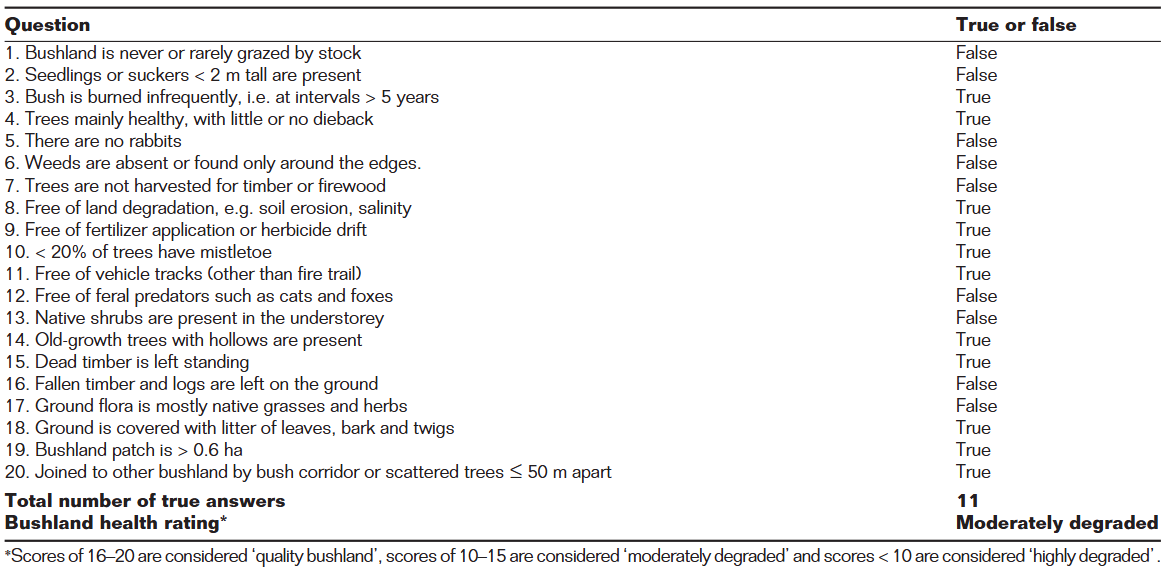
\includegraphics[width=\textwidth]{Included_Images/manual_survey.png}
    \caption{An example of manual survey questionnaires \cite{Gibbons2006}.}
    \label{manual survey}
\end{figure}

Remote sensing can be defined as the acquisition of an object's measurements
without coming into direct contact with said object, effectively minimizing the
need for manual involvement on-site \cite{campbell2011introduction}.
Specifically, remote sensing relies on information derived from different
measurements of energy reflected from the object of interest
\cite{campbell2011introduction}. As a result, remote sensing methods enable
efficient, large-scale monitoring of vegetation, with varied resolutions
depending on the sensing platform used.

\begin{figure}[H]
    \centering
    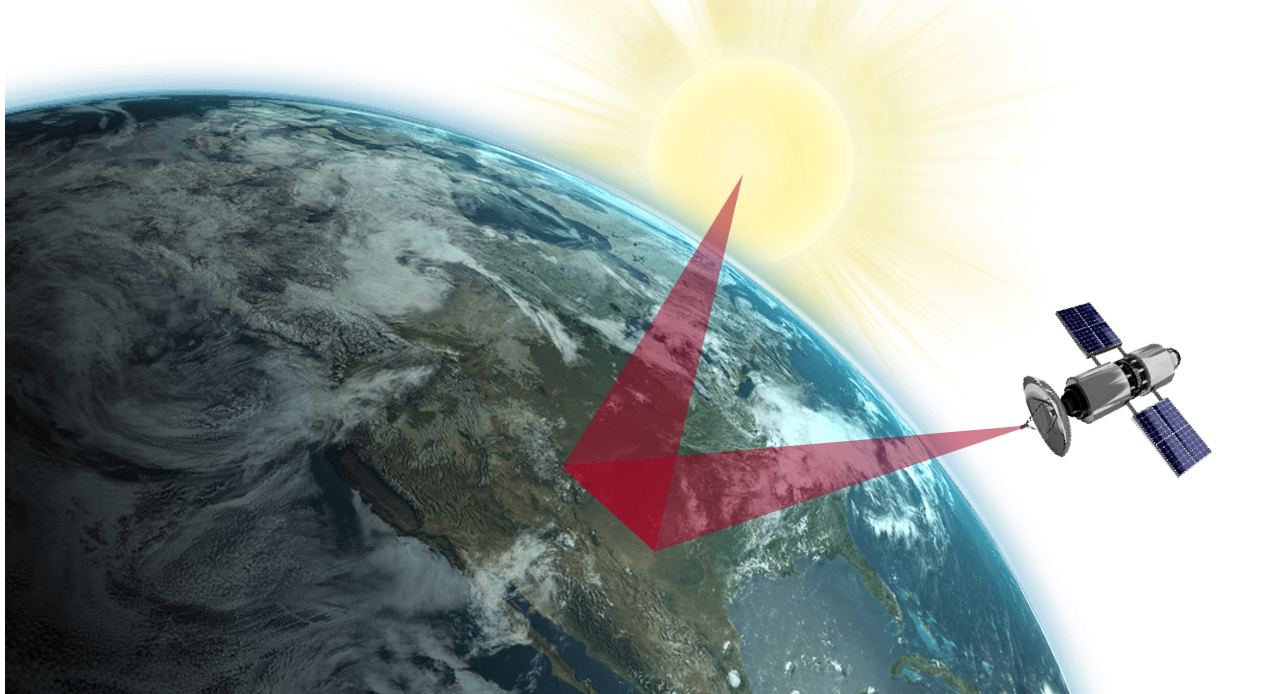
\includegraphics[width=0.75\textwidth]{Included_Images/remotesensing_schematic.png}
    \caption{A schematic illustration of satellite remote sensing.}
\end{figure}

In the context of surveying terrestrial vegetation, the remote sensing methods
could be classified based on the distance between the target object and the
measurement sensor into two categories: 1) space-borne and 2) airborne remote
sensing. Space-borne remote sensing involves the use of instruments onboard
orbiting satellites, including spectral and hyperspectral cameras
\cite{Qian2022}, synthetic aperture radar (SAR) \cite{Hu2025}, and space-borne
Light Detection and Ranging (LiDAR) sensors \cite{Bergen2009}. Due to the wide
coverage and availability of space-borne data, large-scale terrestrial changes
over time could be captured, enabling the continuous monitoring of macro-scale
ecosystems \cite{Khan2024}. Compared to space-borne systems, airborne remote
sensing can provide significantly improved spatial resolution and assessment
flexibility through the integration of sensors onboard manned aircraft or UAVs
\cite{Khan2024}. Although limited by coverage area, airborne remote sensing can
provide timely information for addressing regional emergencies such as pest
\cite{Wulder2006} or wildfire \cite{Arroyo2008} outspreads since the systems
could be deployed on-demand. In UAV-based remote sensing particularly, this
temporal flexibility is further complemented with the benefit of low operational
cost, rendering it an ideal platform for monitoring regional and urban
vegetation \cite{Tang2015}. 

Conventionally, UAV remote sensing platforms carry similar instruments to that of other remote sensing systems, including radar, LiDAR, and multi-spectral or hyperspectral imagery sensors \cite{Tang2015}. Among these sensing methods, LiDAR is particularly suitable for vegetation monitoring as it is able to capture three-dimensional structural information about the environment. With that, valuable spatial data such as canopy height, density, and terrain structure, can be obtained for urban forestry management. Unlike imaging instruments which are susceptible to the influence of lighting and weather, LiDAR measurements are less sensitive to varying lighting conditions and more robust against visually repetitive scenes \cite{Wu2024, jiang2025gps}. Thereby providing reliable geometric reference of tree canopies. 

However, standalone LiDAR measurements are insufficient in a UAV-based applications as the sensor is continuously moving and does not provide spatial context \cite{wang2026multi}. Therefore, it is necessary to integrate LiDAR sensing with a Simultaneous Localization and Mapping (SLAM) framework to estimate the UAV trajectory while incrementally constructing a 3D point cloud map of the environment. Even so, LiDAR-based SLAM primarily relies on relative motion between consecutive scans to estimate the object's trajectory. Given that, the 3D map is susceptible to cumulative drift over time especially in large-scale or long-duration operations. To address this limitation, external global references such as GPS measurements can be integrated into the SLAM framework to provide absolute positioning constraints. This fusion combines the global stability of GPS with the local accuracy of LiDAR, enabling the UAV to maintain robust localization while constructing accurate 3D representations of forest environments.
\begin{figure}[H]
    \centering
    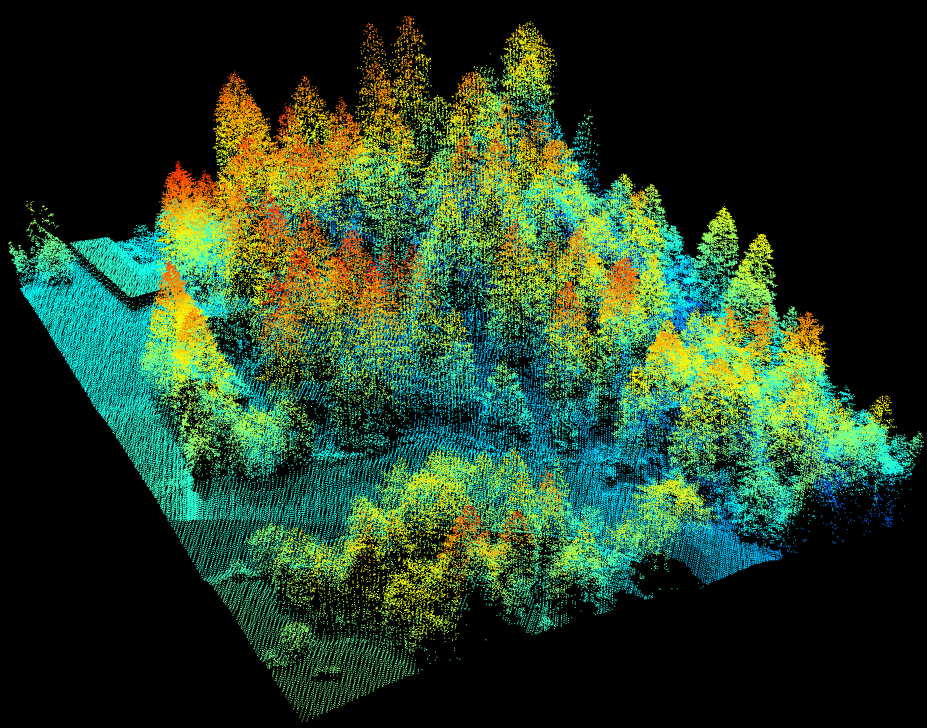
\includegraphics[width=0.7\linewidth]{Included_Images/Nuage_Lidar-003.png}
    \caption{LiDAR point clouds of vegetation.}
\end{figure}

Despite being a relatively robust sensor for vegetation remote sensing, LiDAR devices may occasionally face difficulties penetrating through dense canopy \cite{Su2007}. Therefore, it is critical to explore a
robust sensing technique that is suitable for UAVs in terms of payload and power
consumption to complement the existing instruments. 
\begin{figure}[H]
    \centering
    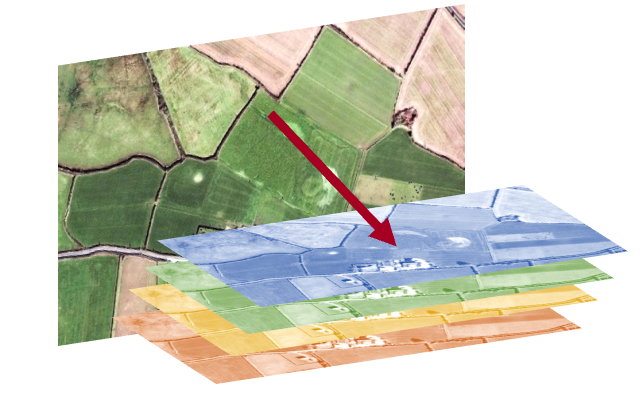
\includegraphics[width=0.7\linewidth]{Included_Images/Spectral_camera_image.png}
    \caption{Spectral Imagery as one of the common remote sensing instruments found on UAV platforms.}
\end{figure}


Recently, the technique of GNSS-R is receiving increasing interest in the field
of remote sensing. GNSS-R exploits the L-band signals transmitted from Global
Navigation Satellite Systems (GNSS) that are then scattered on different terrain
surfaces of the Earth \cite{Jin2024}. Then, the reception of reflected GNSS
signals can provide information regarding the properties of the signal reflector
on land \cite{Jin2024}. As signals of opportunity conventionally dedicated to
Positioning, Navigation, and Timing (PNT) applications, GNSS is capable of
providing real-time measurements regardless of time, location, and weather
\cite{Jin2024}. Additionally, as a bi-static system where signal transmitters
are separated from receivers, GNSS-R is exempt from the need of dedicated
transmitter-receiver instruments that are crucial to mono-static radar systems
\cite{Jin2010}. Instead, any consumer-grade receivers capable of receiving
reflected GNSS signals could be used for GNSS-R remote sensing, further
demonstrating GNSS-R's applicability onboard low-cost remote sensing systems
such as a UAV. 

\begin{figure}[H]
    \centering
    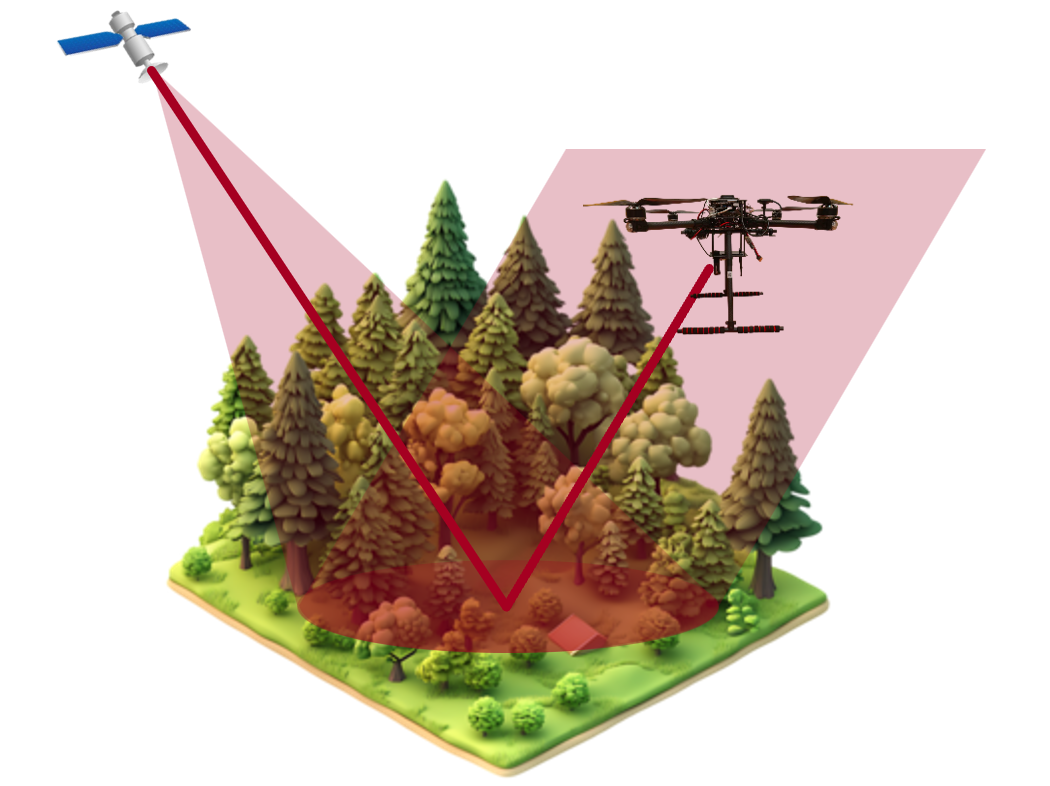
\includegraphics[width=0.6\textwidth]{Included_Images/GNSS-R schematic.png}
    \caption{A schematic illustration of signal propagation path within a UAV-based GNSS-R system.}
\end{figure}

Recent research has demonstrated the potential of integrating GNSS-R techniques
with UAVs through a UAV-based GNSS-R system for water body detection and flood
mapping \cite{app10010210}. Not only does this application demonstrate the
capability of obtaining high-resolution, but it also establishes UAV-mounted
GNSS-R as a promising tool for monitoring dynamic environmental conditions.
However, the effectiveness of UAV-based remote sensing is inherently tied to the
efficiency of the UAV flight path. Traditionally, UAV remote sensing missions
rely on predefined lawnmower patterns or manual piloting, which is not optimal
for dense vegetation or for identifying complex GNSS signal-reflected areas
\cite{GALCERAN20131258}. Consequently, path planning serves as a critical bridge
in vegetation monitoring by providing optimized flight paths in order to
retrieve ground parameters. Therefore, implementing coverage path planning (CPP)
algorithms is necessary for autonomous navigation to survey the entire area of
interest and consistently receive GNSS-R signals that reflect off the target
area \cite{Cabreira2019}.

For GNSS-R applications specifically, the geometry of the reflected signal is
highly dependent on the relative positions of the GNSS satellites and the
receiver. Consequently, an optimized trajectory can be designed to navigate
through these specular reflection zones. While manual vegetation monitoring
flights provide a straightforward solution, having an autonomous system that
detects reflected areas significantly enhances data collection efficiency.
Figure \ref{fig:cpp_over_vegetation} illustrates a coverage path planning result
over a vegetation area after identifying the specular reflection zones.

\begin{figure}[H]
    \centering
    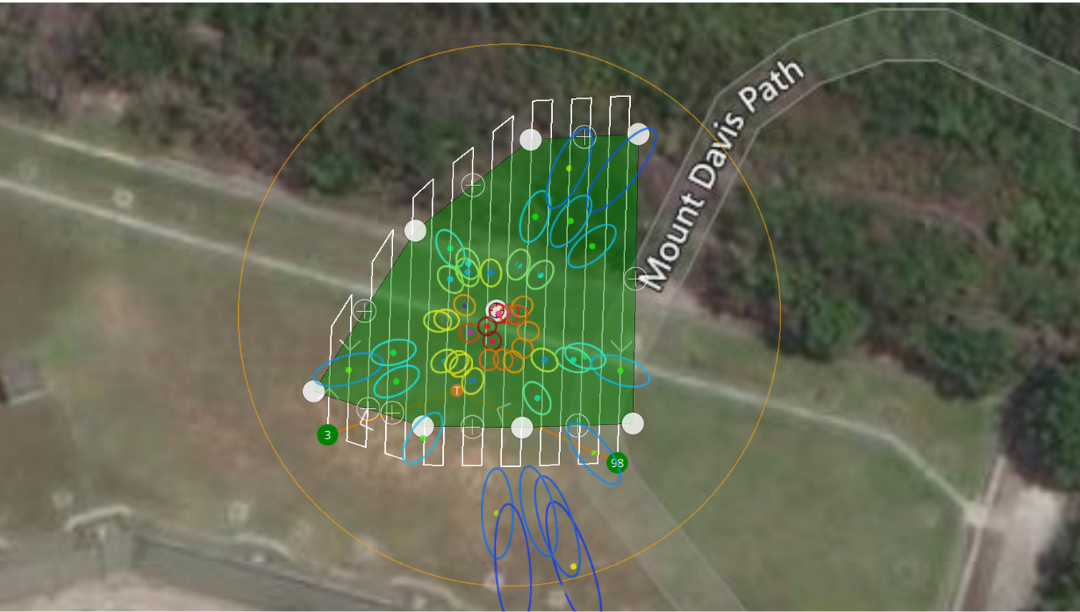
\includegraphics[width=0.8\textwidth]{Included_Images/cpp_over_vegetation.png}
    \caption{Coverage path planning result over a vegetation}
    \label{fig:cpp_over_vegetation}
\end{figure}

The combination of autonomous path planning and remote sensing lays the
groundwork for various data fusion methods. By utilizing LiDAR-based
Simultaneous Localization and Mapping (SLAM), a UAV can simultaneously navigate
an unknown canopy and generate a high-resolution map of the
vegetation. This point cloud map provides the necessary context for interpreting
GNSS-R signals, allowing researchers to correlate signal strengths with
vegetation characteristics. Therefore, the development of an intelligent
trajectory planning framework is not merely a logistic solution but also an
innovative solution that aims to enhance terrestrial remote sensing.

As a result, this project aims to address this gap through both the development of
a robust GNSS-R framework for vegetation remote sensing and the integration of
optimal trajectory planning and environment mapping. An additional LiDAR-based
3D canopy map will also provide the critical spatial reference to validate any
vegetation parameters obtained through the GNSS-R framework.

In summary, this project will integrate the technologies of autonomous
navigation, LiDAR SLAM, GNSS-R, and machine learning, to achieve an intelligent
and structured remote sensing system for vegetation monitoring. The main
objectives of this project are as follows:
\begin{enumerate}
\item To introduce an autonomous path planning framework dedicated for UAV-based
GNSS-R remote sensing. The framework aims to identify potential vegetation
areas, deduce optimal GNSS-R detection areas, and generate accurate trajectories
for UAV navigation during data collection. Consequently, the proposed system
enables the UAV to autonomously acquire high-quality GNSS raw data for
environmental monitoring.
\item To establish a detailed 3D canopy map using LiDAR-based SLAM, providing a
spatial validation reference for the 2D vegetation features detected by GNSS-R.
This involves creating a modular SLAM system, incorporating LiDAR odometry as
the front-end and GPS-coupled Pose Graph Optimization (PGO) SLAM as the
back-end. As a result, an accurate vegetation map could be generated to
complement the GNSS-R vegetation monitoring system.
\item To analyze and model the correlations between signal propagation
parameters retrieved through GNSS-R and ground parameters. This involves
collecting and post-processing raw GNSS data, extracting GNSS signal
measurements, and analyzing GNSS signal parameters with respect to ground
regions reflecting the signal. Ultimately, such correlation models are used to
deduce and inform ground vegetation conditions given the GNSS signal properties
received onboard the UAV.
\item To classify signals reflected by vegetation and predict vegetation
boundaries based on raw GNSS data using a machine-learning-based approach.
Through decision tree-based classification, tree-reflected signals and
ground-reflected signals could be identified, which will be used to predict the
vegetation boundary. At last, the predicted vegetation boundary could be used to
cross-validate results obtained from the GNSS-R framework, enhancing the
robustness of the vegetation monitoring system.
\end{enumerate}

Additionally, the code scripts of this project are organized in various GitHub
repositories, which corresponds to the four objectives of this project.
Specifically: 
\begin{itemize}
    \item Path Planning: \url{https://github.com/sashenkagamage/canopix.ai} 
    \item LiDAR SLAM: \url{https://github.com/A4paper2003/catkin_scpgo_ws}
    \item GNSS-R: \url{https://github.com/zhlouise/UAV_GNSS-R}
    \item Machine Learning: \url{https://github.com/gd-Sahat/FYP-ML/tree/main}
\end{itemize}

This report is structured as follows: Section 3 introduces the logical and
physical system architecture adopted in this project, followed by four core
sections covering UAV path planning (Section 4), LiDAR SLAM (Section 5), GNSS-R
(Section 6), and machine learning (Section 7), respectively. Within each of the
four core sections, literature review, methodology, result and discussion are
included to clearly present the work completed in each area. This report then
concludes with sections on experiments conducted (Section 8), case study of
selected experiments (Section 9), conclusion (Section 10), and project
management (Section 11).


% --- System Architecture ---
\newpage
\section{System Architecture}

\subsection{Logical Architecture}
With regard to the project objectives, four key components comprise the system
architecture: path planning, LiDAR SLAM, GNSS-R, and machine learning, as
illustrated in Figure \ref{System Architecture}. Here, the path planning
processes are indicated in green, LiDAR SLAM processes in orange, GNSS-R
processes in blue, and machine learning processes in yellow.

\begin{figure}[H]
    \centering
    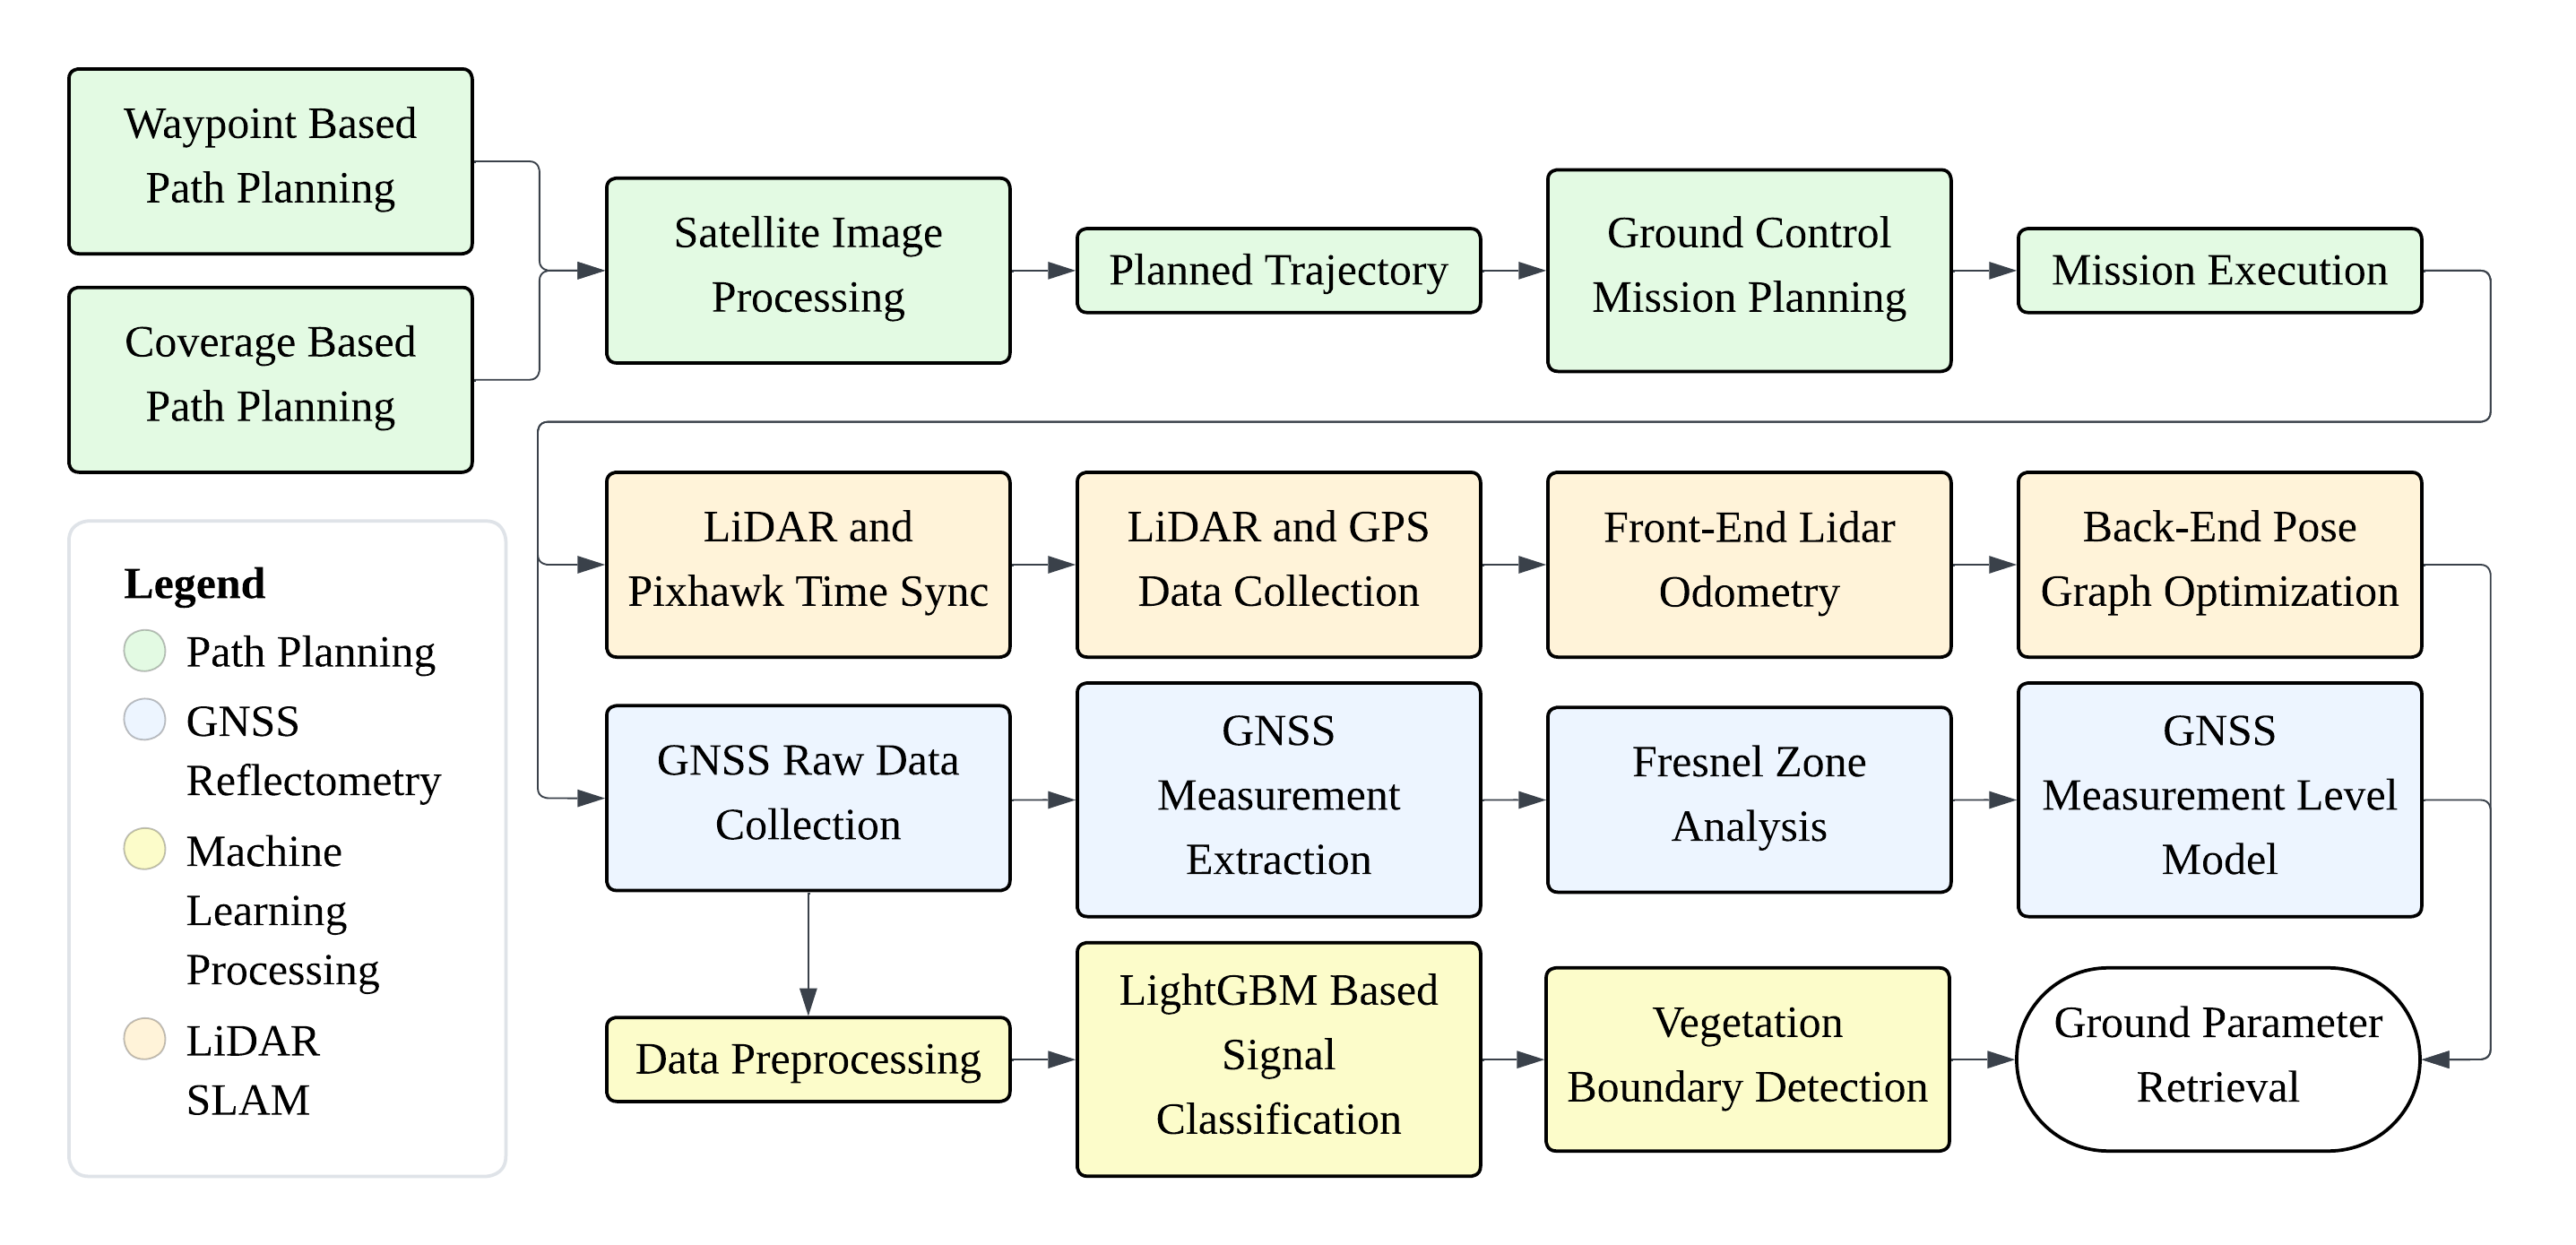
\includegraphics[width=\textwidth]{Included_Images/System_Architecture.png}
    \caption{System Architecture}
    \label{System Architecture}
\end{figure}

First, both waypoint-based and coverage-based path planning algorithms will be
adopted to navigate the UAV platform for specific monitoring missions, while
satellite imagery will be used for identifying vegetation area targets for
sensing. Additionally, potential GNSS signal reflection regions will also be
taken into consideration while designing the flight trajectory. Lastly, the
ground control station will plan and execute the flight mission for collecting
both the raw GNSS data and LiDAR point cloud data over the target vegetation
area.

After the flight, the LiDAR data will be synchronized with timestamps obtained
from the flight controller's GPS module. Then, both LiDAR and GPS data will be
collected and used for the generation of a 3D vegetation map. This will be
achieved through a modular LiDAR framework, utilizing LiDAR odometry as the
front-end and Pose Graph Optimization (PGO) SLAM as the back-end. As a result, the 3D
vegetation map generated within the LiDAR environment can be used to
cross-validate the ground parameters retrieved by GNSS-R and machine learning
models.

The raw GNSS data collected during the flight mission will be post-processed
into two key measurements: 1) the signal's carrier to noise ratio ($C/N_0$), and
2) the excess pseudorange delay of the reflected signal after compensating for
the delay caused by geometrical reflection. These measurements are then analyzed
in correlation with the ground regions that the signals reflected off from - the
First Fresnel Zones, while any correlation between GNSS measurements and ground
parameters will be modelled both quantitatively and qualitatively. Ultimately,
such models will be used to retrieve highly correlated ground parameters from
key GNSS signal measurements.

Lastly, machine learning methods will be adopted to process the collected GNSS
data. A trained LightGBM model will be used to classify the GNSS signals
according to the signal reception scenarios: direct open sky reception, signals
reflected from vegetation, and signals reflected from bare ground. The signal
classification results, combined with the Fresnel Zone locations, will be used
to detect vegetation boundary and cross-validate the ground parameters retrieved
from the GNSS-R framework.

\subsection{Physical Architecture}
An integrated UAV platform is built and utilized for achieving each of the four
project objectives. As shown in Figure \ref{UAV Platform Diagram}, the platform
is built on a Holybro X650 drone frame, integrated with a Pixhawk 6C flight
controller and a pair of SiK telemetry radio for ground control communication. A
pair of U-blox F9P GNSS receivers with L1/L2 band antenna are installed onboard,
with one upward-facing RHCP antenna (zenith) located at the top and one
downward-facing LHCP antenna (nadir) located at the bottom. As a result, both
the direct RHCP signal and the ground-reflected LHCP signal could be received
simultaneously for further analysis. Additionally, an onboard Nvidia Jetson Orin
Nano serves as the primary computer responsible for the control and logging of
LiDAR and GNSS receiver data. The system is further supported by an additional
GPS module directly connected to the flight controller, enabling both manual and
autonomous flight operations.

\begin{figure}[H]
    \centering
    \includegraphics[width=\textwidth]{Included_Images/UAV_Setup.png}
    \caption{UAV Platform and Onboard Setup}
    \label{UAV Platform Diagram}
\end{figure}

% --- Path Planning ---
\section{Path Planning}

\subsection{Literature Review}
Path planning is a technique that is used in navigating a robot autonomously
from an origin to a destination via a collision-free route. It is primarily a
geometric problem that generates a path according to a given sequence of
waypoints, without accounting for variations over time
\cite{Gasparetto2015}. Currently, our research focuses on implementing path
planning for the autonomous navigation of an Unmanned Aerial Vehicle (UAV) in
outdoor environments.

The earliest sensor-based, obstacle-avoiding path planning algorithms are known
as Bug1 and Bug2 algorithms \cite{choset2005principles}, which are designed to
first navigate around an obstacle and then determine the shortest path around
the obstacle to reach the goal. However, these algorithms are used
in scenarios where the robot has no map (i.e., an unknown environment). With the
rise of SLAM techniques, maps of the navigation environment can be generated,
which enabled the transition to map-based path planning methods. Therefore, the
conventional grid-based path planning algorithms will be integrated in this
project, which enables the identification of potential vegetated areas for
further GNSS-R surveying.

One of the primary reasons for utilizing autonomous navigation and path planning
in our UAV system is that it is scalable across vegetation monitoring, providing
accurate and precise navigation in fragmented urban forests. To develop path
planning mechanisms, we conducted our literature review across four different
path planning approaches. 

\begin{enumerate} 
    \item \textbf{Search-based algorithms}: Dijkstra algorithm and A* algorithm.
    \item \textbf{Sampling-based algorithms}: RRT (Rapidly-exploring Random Tree)
    algorithm, RRT*, and PRM (Probabilistic Roadmap) algorithm.
    \item \textbf{Artificial Intelligence-based algorithms}: Soft-Actor-Critic.
    \item \textbf{Cell Decomposition Algorithms}: Boustrophedon Cell Decomposition.
\end{enumerate}

\paragraph{Search-based algorithms} ~\\
Dijkstra's algorithm is one of the major search-based algorithms, that finds the
shortest path from a given starting point to a given ending point. The algorithm
explores this path by simultaneously finding the shortest path from a given
starting node to all points in the graph \cite{javaid2013understanding}.
However, finding the optimal path across all the points in the map incurs high
computational cost. Therefore, it is impractical to use for real-time UAV path
planning. 

To address the limitations of Dijkstra’s algorithm, scientists developed another
search-based algorithm called the A* (A-star) algorithm. The A* algorithm is one of
the most common path planning algorithms, which can be applied to grid-based or
geometrical configuration spaces \cite{Astar_simulation}. This algorithm
combines the shortest path calculation in Dijkstra’s algorithm and heuristic
searching. The heuristic cost is known as the estimated cost from the current
node to the end node. The A* algorithm is better in terms of reducing the search
space compared to the Dijkstra algorithm. However, it requires accurate
heuristics to determine the shortest path and has a large computation time
depending on the number of cells in the map \cite{DUCHON201459}.  

\paragraph{Sampling-based algorithms} ~\\
Due to the excessive amount of computational power consumed by search-based
algorithms \cite{karaman2011samplingbasedalgorithmsoptimalmotion}, sampling-based
algorithms have been proposed and have performed effectively in high-dimensional
spaces, attracting significant attention across several decades
\cite{Kavraki, kavraki_etal}. The most common sampling-based algorithms are
RRTs and PRM algorithms.

The RRT algorithm operates by iteratively sampling random states within the
configuration space and extending the nearest existing node in the tree toward
these samples. This sampling-based approach allows the algorithm to spread like a
tree and rapidly explore the state space and eventually connect to the goal. 

Additionally, RRT effectively handles systems with differential constraints
\cite{anytimeRRT}, making it a suitable algorithm for state-of-the-art robotics.
Although RRT quickly computes the path between the starting and ending points,
it does not guarantee the shortest path. This was proven by Karaman and Frazzoli
\cite{karaman2010incrementalsamplingbasedalgorithmsoptimal}, stating that there
is a zero probability of the RRT algorithm converging to an optimal solution.
Therefore, the RRT*, an optimal version of the RRT algorithm, was proposed. 
\begin{figure}[H]
    \centering
    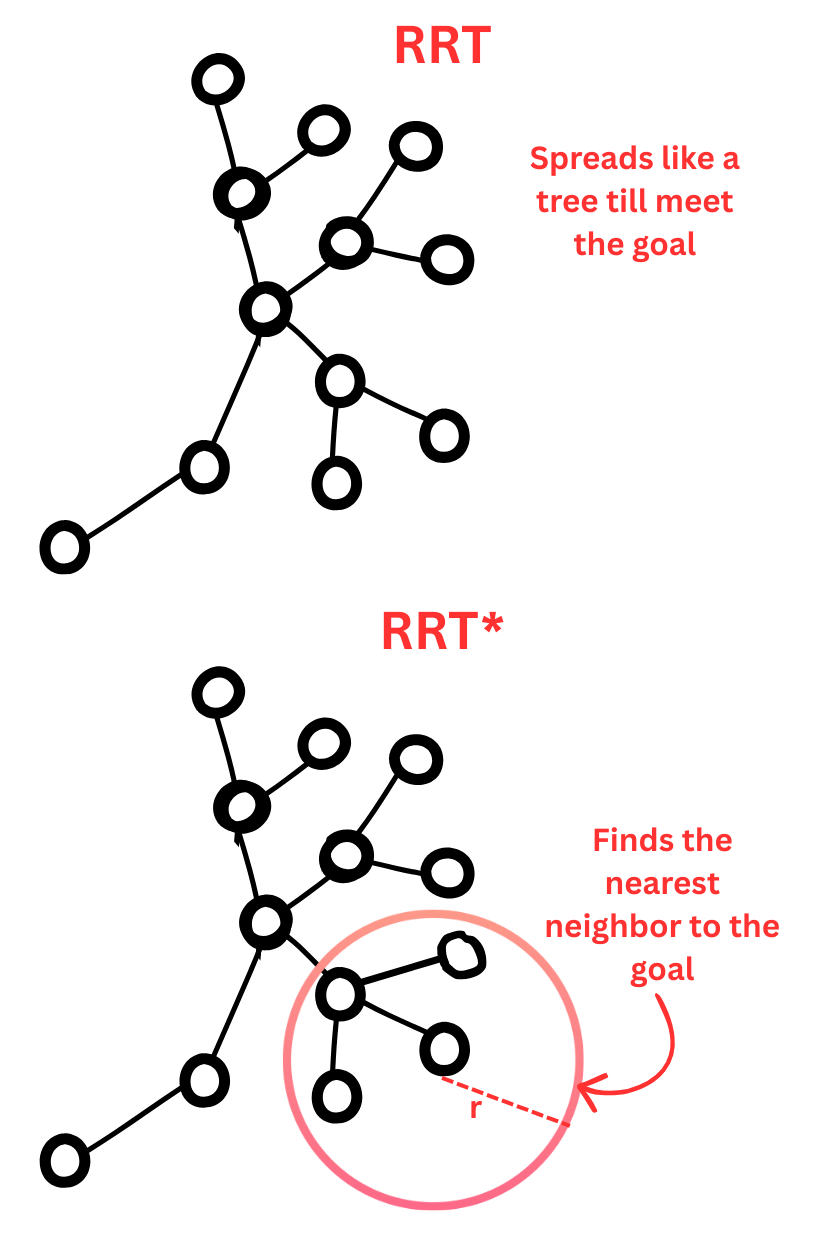
\includegraphics[width=0.38\linewidth]{Included_Images/rrt_vs_rrtstar.png}
    \caption{RRT vs RRT*}
    \label{fig:rrt_vs_rrtstar}
\end{figure}
As shown in Figure \ref{fig:rrt_vs_rrtstar}, RRT* incorporates a rewiring step
within a neighbor radius $r$, ensuring that the path improves as the number of
iterations increases \cite{karaman2011samplingbasedalgorithmsoptimalmotion}. As
the number of iterations increases, RRT* performance improves, while the path
becomes more jagged with each iteration \cite{noreen2016comparison}. Moreover,
PRM is another type of sampling-based algorithm that has a network of possible
paths in the freely available space. By creating a network among the available
spaces, the PRM increases the path-finding speed by converting the map into a
graph \cite{PRM}.

\paragraph{AI-based algorithms} ~\\
In recent years, deep reinforcement learning methods have been employed to
address task allocation and path planning problems in autonomous vehicles
\cite{RL-path-planning}. Multi-UAV path planning systems have been deployed as
multi-agent reinforcement learning problems \cite{SAC-path-planning}. Recent
studies have merged the Soft-Actor-Critic (SAC) reinforcement learning algorithm
with a sampling-based path planning algorithm to design adaptively informed
trees (AIT*) \cite{ait}. 
SAC learns a policy that specifies a given state and
the corresponding action to be taken. With the correct reward design (e.g.,
penalties for collisions, rewards for reaching the goal), SAC can learn to
generate collision-free trajectories.

Table \ref{tab:algorithms_comparison} summarizes the advantages and
disadvantages of the search-based, sampling-based, and AI-based path planning
algorithms. 

\begin{table}[ht]
    \newcolumntype{L}{>{\RaggedRight\arraybackslash}X}
    \caption{Comparison of Waypoint-based Path Planning Algorithms}
    \label{tab:algorithms_comparison}
    \centering
    \footnotesize
    \begin{tabularx}{\linewidth}{@{} l l L L @{}}
        \toprule
        \textbf{Category} & \textbf{Algorithm} & \textbf{Advantages} & \textbf{Disadvantages} \\
        \midrule

        % --- SEARCH BASED ---
        \multirow{2}{*}{\textbf{Search-based}} & \textbf{A*} &
        % [nosep] removes all vertical space, [leftmargin=*] aligns bullets to text
        \begin{itemize}[nosep, leftmargin=*, label=\textbullet]
            \item Guarantees shortest path if heuristic is accurate.
            \item Reduces the search space compared to Dijkstra.
        \end{itemize} &
        \begin{itemize}[nosep, leftmargin=*, label=\textbullet]
            \item High computational cost in large spaces.
            \item Needs accurate heuristics.
            \item Poor performance in dynamic environments.
        \end{itemize} \\
        \addlinespace[4pt] % Adds a tiny gap between rows instead of a line

        & \textbf{Dijkstra} &
        \begin{itemize}[nosep, leftmargin=*, label=\textbullet]
            \item Finds optimal path.
            \item Simple to implement.
        \end{itemize} &
        \begin{itemize}[nosep, leftmargin=*, label=\textbullet]
            \item Computationally expensive.
            \item Impractical for real-time UAVs.
        \end{itemize} \\
        \midrule

        % --- SAMPLING BASED ---
        \multirow{2}{*}{\textbf{Sampling-based}} & \textbf{RRT} &
        \begin{itemize}[nosep, leftmargin=*, label=\textbullet]
            \item Fast exploration of high-dim spaces.
            \item Good for unknown maps.
        \end{itemize} &
        \begin{itemize}[nosep, leftmargin=*, label=\textbullet]
            \item No guarantee of optimal path.
            \item Paths are often jagged and require smoothing.
        \end{itemize} \\
        \addlinespace[4pt]

        & \textbf{RRT*} &
        \begin{itemize}[nosep, leftmargin=*, label=\textbullet]
            \item Paths improve over time.
            \item Handles complex spaces.
            \item Retains the exploration ability of RRT.
        \end{itemize} &
        \begin{itemize}[nosep, leftmargin=*, label=\textbullet]
            \item Computational cost is higher than RRT.
            \item Slower convergence.
        \end{itemize} \\
        \midrule

        % --- AI BASED ---
        \multirow{1}{*}{\textbf{AI-based}} & \textbf{SAC} &
        \begin{itemize}[nosep, leftmargin=*, label=\textbullet]
            \item Learns adaptive policies.
            \item Handles continuous control.
            \item Robust in dynamic, uncertain environments.
            \item No explicit map needed.
        \end{itemize} &
        \begin{itemize}[nosep, leftmargin=*, label=\textbullet]
            \item Requires large training data and simulation
            \item Reward design is non-trivial.
            \item No hard optimality guarantee.
            \item Complex to implement
        \end{itemize} \\
        \bottomrule
    \end{tabularx}
\end{table}

\paragraph{Decomposition-based algorithms} ~\\
One of the primary reasons for using cell decomposition methods in our project
is to cover fragmented areas in the vegetation environment. In cell
decomposition methods, the robot's navigation space is divided into several
regions, called cells \cite{Gasparetto2015}. The decomposition process can
be explained as follows: dividing the free space into several polygons, creation
of a connectivity graph, identification of regions to be crossed, and generation
of the path.  Figure \ref{fig:cell_decomposition} shows the detailed steps
of the exact cell decomposition process. In our system, we utilize exact cell
decomposition, specifically boustrophedon decomposition, for coverage path
planning. 
\begin{figure}[H]
    \centering
    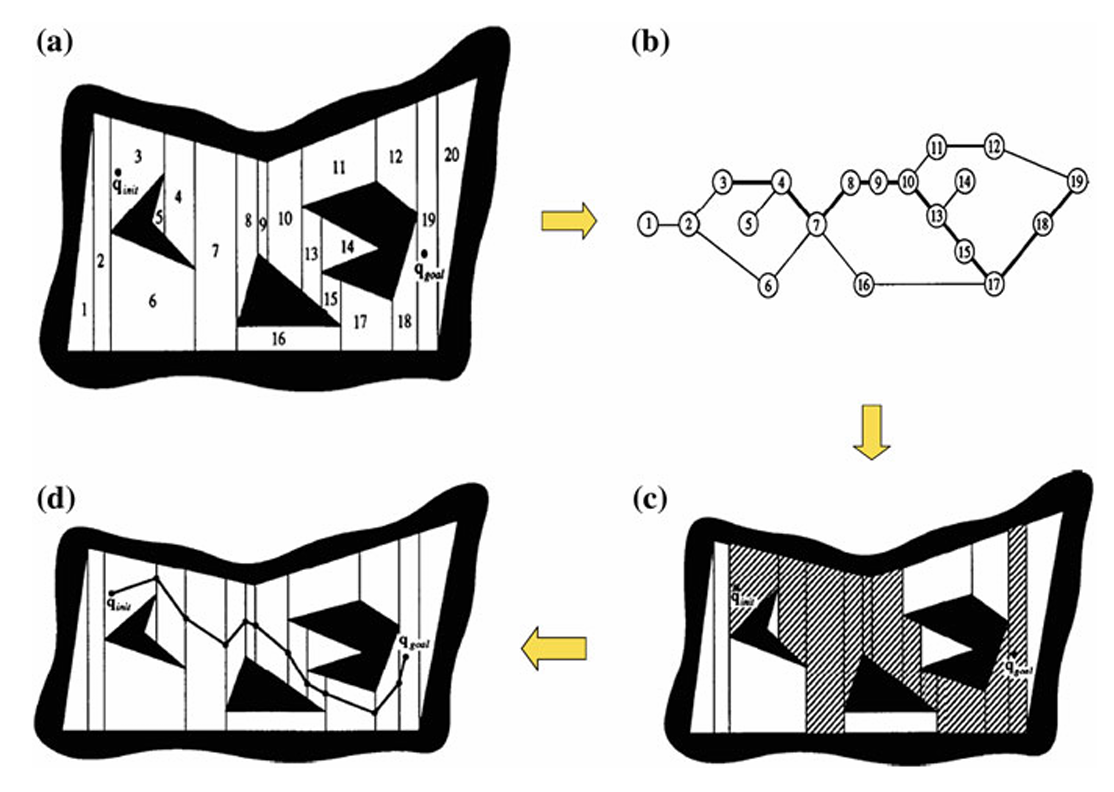
\includegraphics[width=\linewidth]{Included_Images/cell_decomposition.png}
    \caption{Exact Cell Decomposition Process \cite{choset2005principles}}
    \label{fig:cell_decomposition}
\end{figure}
The boustrophedon cellular decomposition is a common algorithm that breaks down
the robot’s free space into cells and covers each cell with a motion of back-and-forth \cite{choset2000coverage}. Compared to spiral patterns, which cause the
UAV to constantly bank (roll), thereby destabilizing the antenna, using
boustrophedon maintains a stable flight attitude suitable for consistent data
collection. Furthermore, it offers better kinematic feasibility compared to the
jagged paths often produced by standard wavefront algorithms. 

\subsection{Methodology}
As mentioned in the system architecture, path planning focuses on two methods:
Waypoint-Based Navigation and Coverage Path Planning. These methods are crucial
for observing dense forests, enabling maneuvers such as hovering over trees and
surveying the dense canopy to obtain dynamic data for LiDAR SLAM. The detailed
methodologies for each method are presented below.

\subsubsection{Waypoint-based navigation}
Waypoint-based navigation can be achieved through various approaches, such as
search-based algorithms, graph-based algorithms, and Artificial
Intelligence-based algorithms. Since the UAV is designed to hover over dense
vegetation environments and identify potential Fresnel Zones, it primarily needs
to fly outdoors at high altitudes in open spaces. To determine the optimal
algorithm for building an intelligent UAV system, a baseline comparison was
conducted among the Dijkstra algorithm, the A* algorithm, and the RRT
algorithm.

\begin{table}[ht]
    \centering
    \renewcommand{\arraystretch}{1.3} % Adds a little vertical padding for readability
    % 'l' = left align, 'X' = auto-wrap column
    \begin{tabularx}{\textwidth}{@{} l l X X @{}} 
    \toprule
    \textbf{Category} & \textbf{Algorithm} & \textbf{Advantages} & \textbf{Disadvantages} \\ 
    \midrule

    % SEARCH BASED SECTION
    \multirow{10}{*}{\textbf{Search-based}} & \textbf{A*} & 
    \begin{itemize}[leftmargin=*, noitemsep, topsep=0pt]
        \item Shortest path is guaranteed for a given heuristic map.
        \item Reduces computation power and search space compared to Dijkstra.
    \end{itemize} & 
    \begin{itemize}[leftmargin=*, noitemsep, topsep=0pt]
        \item High computational cost in large or continuous spaces.
        \item Poor scalability in dynamic environments.
    \end{itemize} \\ 
    \cmidrule{2-4}
    
    & \textbf{Dijkstra} & 
    \begin{itemize}[leftmargin=*, noitemsep, topsep=0pt]
        \item Designed to find the optimal path. 
        \item Simple to implement.
    \end{itemize} & 
    \begin{itemize}[leftmargin=*, noitemsep, topsep=0pt]
        \item Computationally expensive.
        \item Impractical for real-time UAV planning.
    \end{itemize} \\ 
    \midrule

    % SAMPLING BASED SECTION
    \textbf{Sampling-based} & \textbf{RRT} & 
    \begin{itemize}[leftmargin=*, noitemsep, topsep=0pt]
        \item Fast exploration of high-dimensional spaces.
        \item Perform well in unknown maps.
    \end{itemize} & 
    \begin{itemize}[leftmargin=*, noitemsep, topsep=0pt]
        \item Does not guarantee the optimal path.
        \item Paths are often jagged and require smoothing.
    \end{itemize} \\ 
    \bottomrule
    \end{tabularx}
    \caption{Comparison of Path Planning Algorithms}
    \label{tab:algorithms}
\end{table}

As a result, for a given occupancy grid map, the comparison shows that the A*
algorithm is suitable for offline path planning. Therefore, the system is
designed to perform offline path planning using the A* algorithm. On the other
hand, RRT performs well in dynamic, unknown environments and is suitable for
online path planning. 

\paragraph{A* Algorithm Implementation} ~\\
The A* algorithm is a heuristic, search-based algorithm that calculates the
shortest path from a starting point to a goal. The algorithm first divides the
map into nodes, where each node represents a possible position for the robot to
move. These positions depend on the grid architecture, such as 4-way or 8-way
connected grids.  

In this project, the focus will be on regular 8-way grids that connect nodes
across 26 directions in 3-D space. Each node will be assigned a cost based on
the starting and ending nodes of a given path. A 2-D path illustration of an A*
algorithm is shown in Figure \ref{fig:astar}.
\begin{figure}[ht]
    \centering
    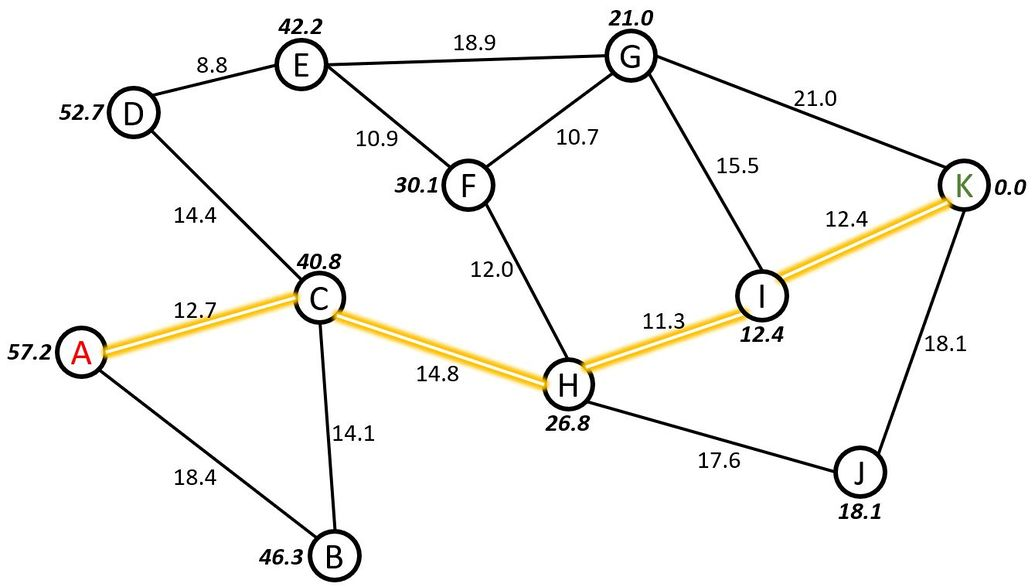
\includegraphics[width=\linewidth]{Included_Images/A-starmap.jpg}
    \caption{Map Highlighting Shortest Path from Node A to Node K.}
    \label{fig:astar}
\end{figure}

\paragraph{A* Algorithm Grid Definition} ~\\
This system utilizes a grid map defined in 3D space, featuring 26-connectivity,
which allows for movement in all straight and diagonal directions. However, to
simplify the initial validation, the algorithm is currently evaluated using a 2D
grid with 8-connectivity. The coordinates of the given map were first converted into
grid node indexes using the \texttt{coord\_to\_index} function. The coordinates
can be defined as world coordinates or image coordinates for a given map image.
An illustration of image coordinates is shown in Figure \ref{fig:image_coordinates}.
\begin{figure}[H]
    \centering
    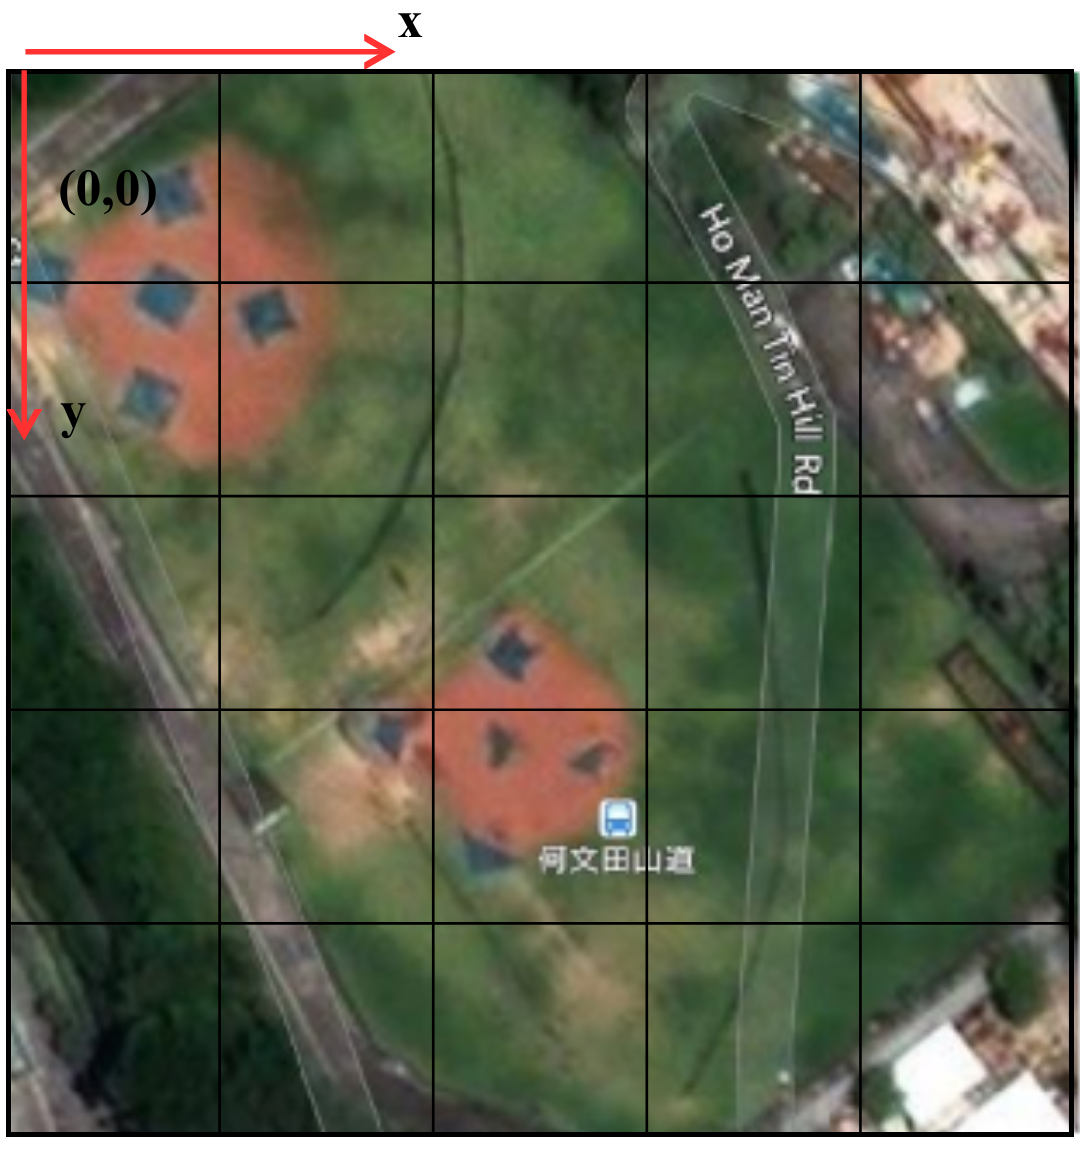
\includegraphics[width=0.5\linewidth]{Included_Images/image_coordinates.png}
    \caption{Image Coordinates System}
    \label{fig:image_coordinates}
\end{figure}
Below is the pseudocode for the \texttt{coord\_to\_index} function:
\begin{singlespace}
\begin{algorithm}[H]
\caption{Coordinate to Grid Index Conversion}
\label{alg:coord_to_index}
\begin{algorithmic}[1]
    \Require $pos$: Real-world coordinate vector $(x, y, z)$
    \Ensure $index$: Integer grid indices $(i, j, k)$
    
    \Function{CoordToIndex}{$pos$}
        \State \Comment{Calculate position relative to the map center}
        \State $pos_{relative} \gets pos - pos_{center}$
        
        \State \Comment{Scale by resolution and round to the nearest integer}
        \State $index \gets \text{round}(pos_{relative} \cdot step_{inv})$
        
        \State \Comment{Apply the center index offset}
        \State $index \gets index + index_{center}$
        
        \State \Return $index$
    \EndFunction
\end{algorithmic}
\end{algorithm}
\end{singlespace}
\paragraph{A* Algorithm Cost Function Implementation} ~\\
The cost function $f(n)$ for each node $n$ is calculated as follows:
\begin{equation}
    f(n) = g(n) + h(n)  
\end{equation}
where:
\begin{itemize}
    \item $g(n)$ is the cost from the starting node to the current node $n$.
    \item $h(n)$ is the estimated cost from node $n$ to the goal node.
    \item $f(n)$ is the total estimated cost of the shortest path node $n$.
\end{itemize}
In this project, the cost $g(n)$ (the cost from starting node to end node) is calculated as the Euclidean distance
between the starting node and the current node $n$.
The Euclidean distance can be calculated as follows:
\begin{equation}
    g(n) = \sqrt{(x_n - x_{start})^2 + (y_n - y_{start})^2 + (z_n - z_{start})^2}  
\end{equation}
where $(x_n, y_n, z_n)$ are the coordinates of the current node $n$ and
$(x_{start}, y_{start}, z_{start})$ are the coordinates of the starting node.
The heuristic cost $h(n)$ is implemented using the diagonal heuristic function. The function has five key steps as follows:
\begin{enumerate}
    \item Calculates the distance differences in each dimension ($dx$, $dy$, $dz$) between the current node and the goal node.
    \item Determines the direction with the minimum change in distance.
    \item The heuristic cost starts at zero and will increment by $\sqrt{3} \cdot \min(dx, dy, dz)$ to account for diagonal movement in 3D space.
    \item The function checks which dimensions still have remaining distance to
    cover. If one dimension has been fully covered (i.e., $dx$, $dy$, or $dz$
    equals zero), it calculates the remaining cost using 2D diagonal movement
    and straight-line movement.
    \item If the three dimensions still have remaining distance, it calculates
    the cost using a combination of 2D diagonal movement and straight-line
    movement for the remaining distances.
\end{enumerate}
Below is the pseudocode for the diagonal heuristic function:
\begin{singlespace}
\begin{algorithm}[H]
\caption{Diagonal Heuristic (3D)}
\label{alg:diagonal_heuristic}
\begin{algorithmic}[1] % The [1] turns on line numbering
    \Require $node_1, node_2$: Current and Goal GridNodes
    \Ensure $h$: Estimated cost to goal
    
    \Function{DiagonalHeuristic}{$node_1, node_2$}
        \State $dx \gets |node_1.x - node_2.x|$
        \State $dy \gets |node_1.y - node_2.y|$
        \State $dz \gets |node_1.z - node_2.z|$
        
        \State \Comment{Find the minimum for 3-D diagonal movement}
        \State $diag_{3d} \gets \min(dx, dy, dz)$
        \State $dx \gets dx - diag_{3d}$
        \State $dy \gets dy - diag_{3d}$
        \State $dz \gets dz - diag_{3d}$
        
        \State $h \gets \sqrt{3} \cdot diag_{3d}$
        
        \State \Comment{Handle remaining 2-D movement}
        \If{$dx = 0$}
            \State $h \gets h + \sqrt{2} \cdot \min(dy, dz) + |dy - dz|$
        \ElsIf{$dy = 0$}
            \State $h \gets h + \sqrt{2} \cdot \min(dx, dz) + |dx - dz|$
        \ElsIf{$dz = 0$}
            \State $h \gets h + \sqrt{2} \cdot \min(dx, dy) + |dx - dy|$
        \Else
            \State \Comment{General case (if dimensions remain)}
            \State $diag_{2d} \gets \min(dx, dy, dz)$
            \State $h \gets h + \sqrt{2} \cdot diag_{2d}$
            \State $remaining \gets (dx - diag_{2d}) + (dy - diag_{2d}) + (dz - diag_{2d})$
            \State $h \gets h + remaining$
        \EndIf
        
        \State \Return $h$
    \EndFunction
\end{algorithmic}
\end{algorithm} 
\end{singlespace}

\paragraph{A* Algorithm Core Logic Implementation} ~\\
The core logic of the A* algorithm involves determining the neighboring nodes,
checking the occupancy of the neighboring nodes, calculating their costs, and
adding the nodes to a separate list that deviates from the list of unexplored
nodes. The algorithm is also responsible for updating its list by adding or
removing neighboring nodes if a better path is found. The core logic works
according to the following steps:

\begin{enumerate}
    \item Initialize the grid, convert the start and end coordinates to grid
    indices, and adjust the indices if the start and end nodes are inside
    obstacles.
    \item Initialize the array to store the exploring nodes, check the node with lowest $f(n)$, skip if already explored.
    \item Move to the next node, check if the current node is the goal node. If so, backtrack and reconstruct the path.
    \item If not, check the neighboring nodes, calculate their tentative costs, and add them to the open set if they are not already explored.
    \item If a node is already in the open set, but a better path is found,
    update the parent node, adjust the $g(n)$ to the lowest cost, and add to
    the queue again with  new priority.
    \item Repeat steps 2-5 till reach the goal, or no path is found.
\end{enumerate}
Below is the flow chart illustrating the core logic of A* algorithm:
\begin{figure}[H]
    \centering
    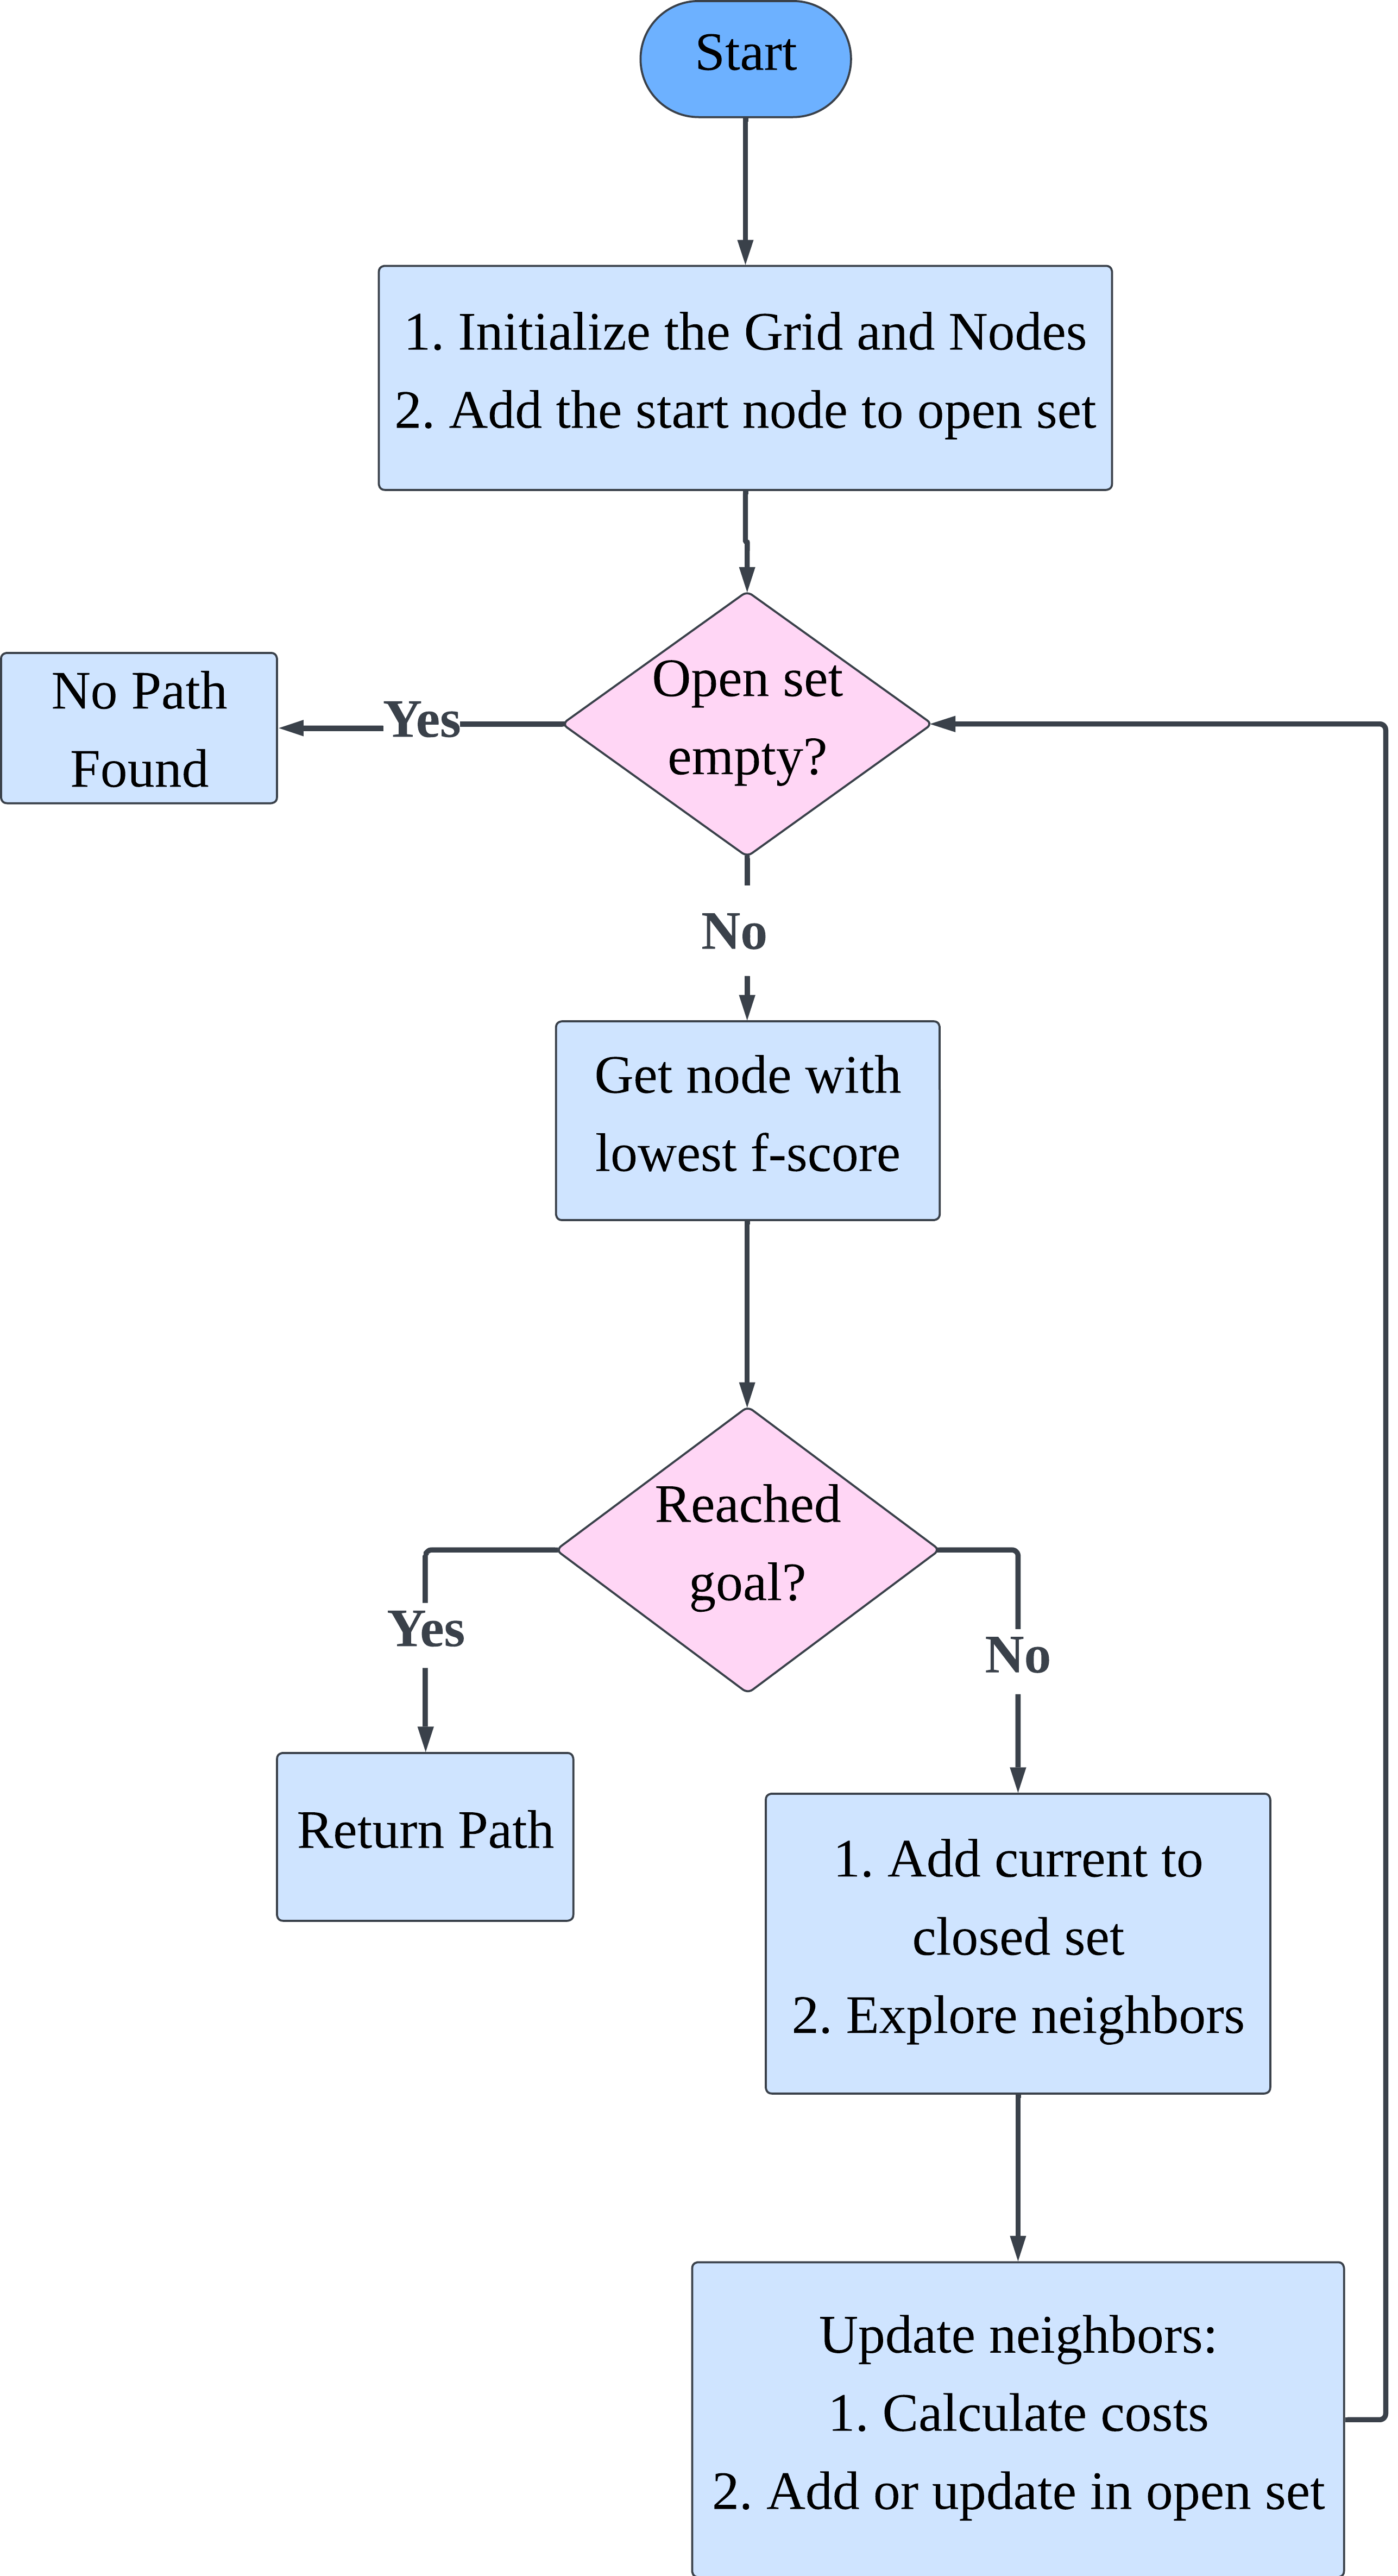
\includegraphics[width=0.5\linewidth]{Included_Images/Astar_flowchart.png}
    \caption{A* Algorithm Core Logic Flowchart}
    \label{fig:astar_flowchart}
\end{figure}

\subsubsection{Coverage Path Planning}
Coverage Path Planning (CPP) is essential for surveying in dense vegetation
areas and for obtaining dynamic data for LiDAR SLAM. In this research,
Boustrophedon Cell Decomposition was implemented as the CPP algorithm. The
decomposition algorithm works by dividing the map into cells based on the
polygonal shape of the map and the obstacles present. After decomposing the map
into cells, the algorithm generates a sweeping path in each cell based on the
given parameters (refer to Figure \ref{fig:boustrophedon}). This sweeping
technique in all the cells ensures that the entire area is covered. Below is a
detailed explanation of how the Boustrophedon Cell Decomposition is implemented
using the framework developed by the Autonomous Systems Lab at ETH Zurich
\cite{B_hnemann_2021}.

\begin{figure}[H]
    \centering
    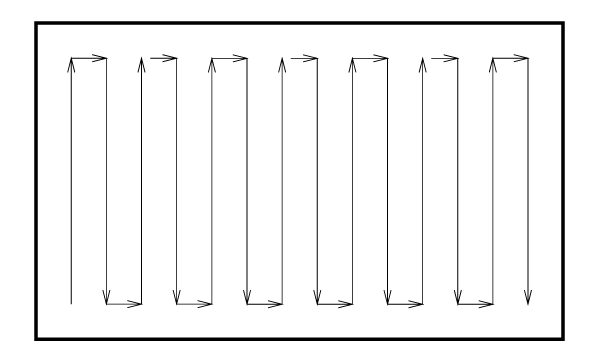
\includegraphics[width=0.5\linewidth]{Included_Images/boustrophedon_path.png}
    \caption{Boustrophedon Cell Decomposition Path Planning Example
    \cite{Choset-1997-16422}}
    \label{fig:boustrophedon}
\end{figure}

\paragraph{Boustrophedon Cell Decomposition Implementation} ~\\
The algorithm decomposes the map (polygonal area) into cells based on three key events:
\begin{itemize} 
    \item \textbf{In Event}: When the sweep line encounters the start of an
    obstacle, the current cell is divided into two new cells. The algorithm is
    defined by an if-else loop that compares the vertices of the obstacle and
    the sweep line intersection. In the IN event, the intersecting vertices move
    in the same direction as the sweep line.

    The conditional logic in an IN event can be interpreted as follows:
\[
    \text{If } \texttt{target\_upper} > \texttt{source\_upper} \text{ and } \texttt{target\_lower} < \texttt{source\_lower}
\]
Figure \ref{fig:in_event} illustrates an example of an IN event:
    \begin{figure}[H]
        \centering
        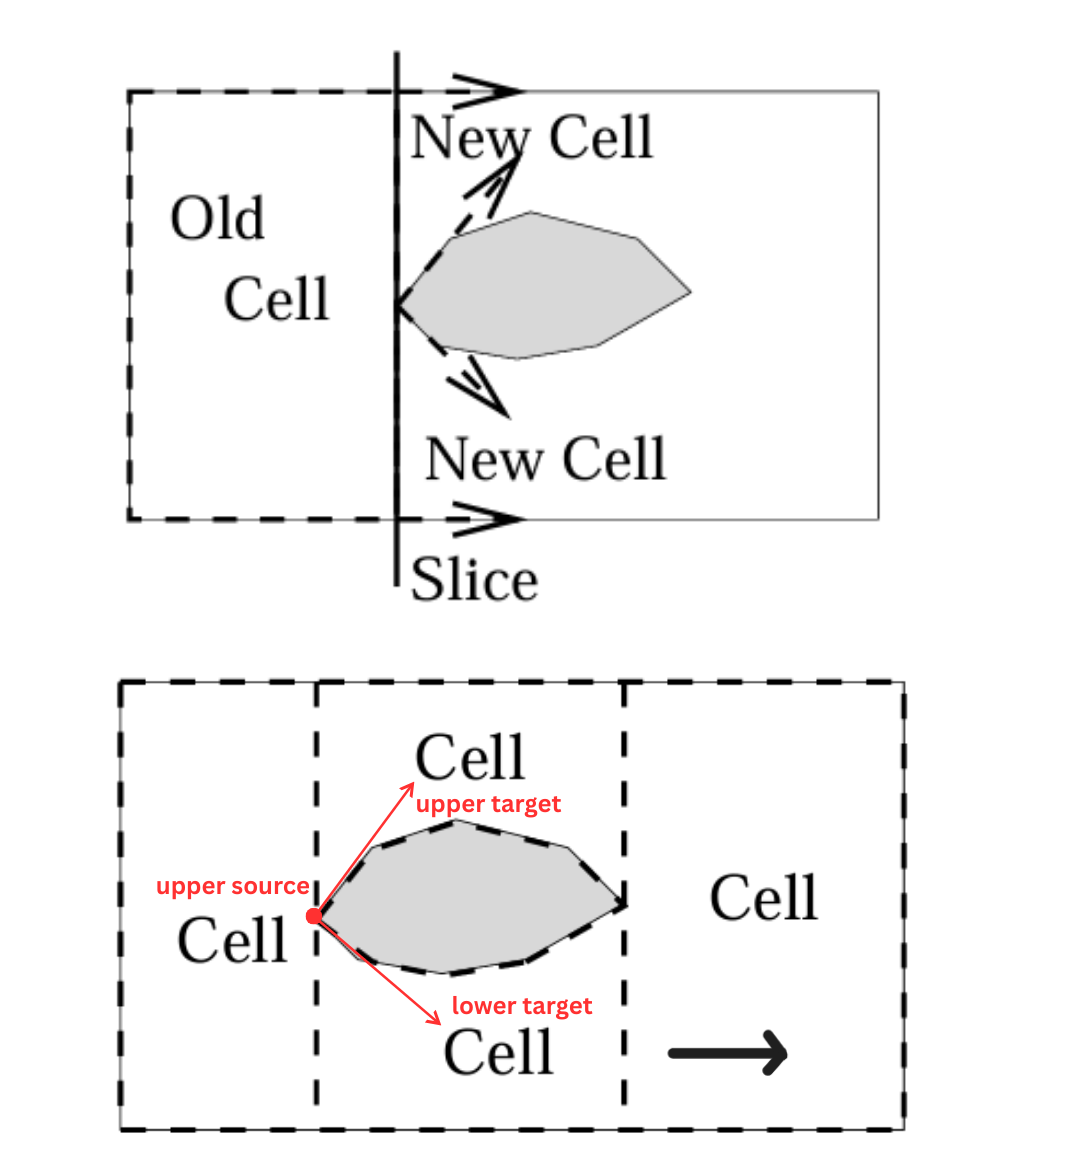
\includegraphics[width=0.65\linewidth]{Included_Images/in_event.png}
        \caption{Boustrophedon Cell Decomposition IN Event Example \cite{Choset-1997-16422}}
        \label{fig:in_event}
    \end{figure}

    \item \textbf{Middle Event}: When the sweep line passes through the obstacle
    and updates its cell status.
    \item \textbf{Out Event}: The sweep line encounters the end of an obstacle,
    and two cells merge into one cell. The algorithm is defined by an if-else
    loop that compares the points of the obstacle's vertices and the
    intersection of the sweep line. In the OUT event, intersecting vertices move
    in the opposite direction of the sweep direction. The conditional logic in an
    OUT event can be interpreted as follows:
\[
    \text{If } \texttt{target\_upper} < \texttt{source\_upper} \text{ and } \texttt{target\_lower} > \texttt{source\_lower}
\]
Figure \ref{fig:out_event} illustrates an example of an OUT event:
    \begin{figure}[H]   
        \centering
        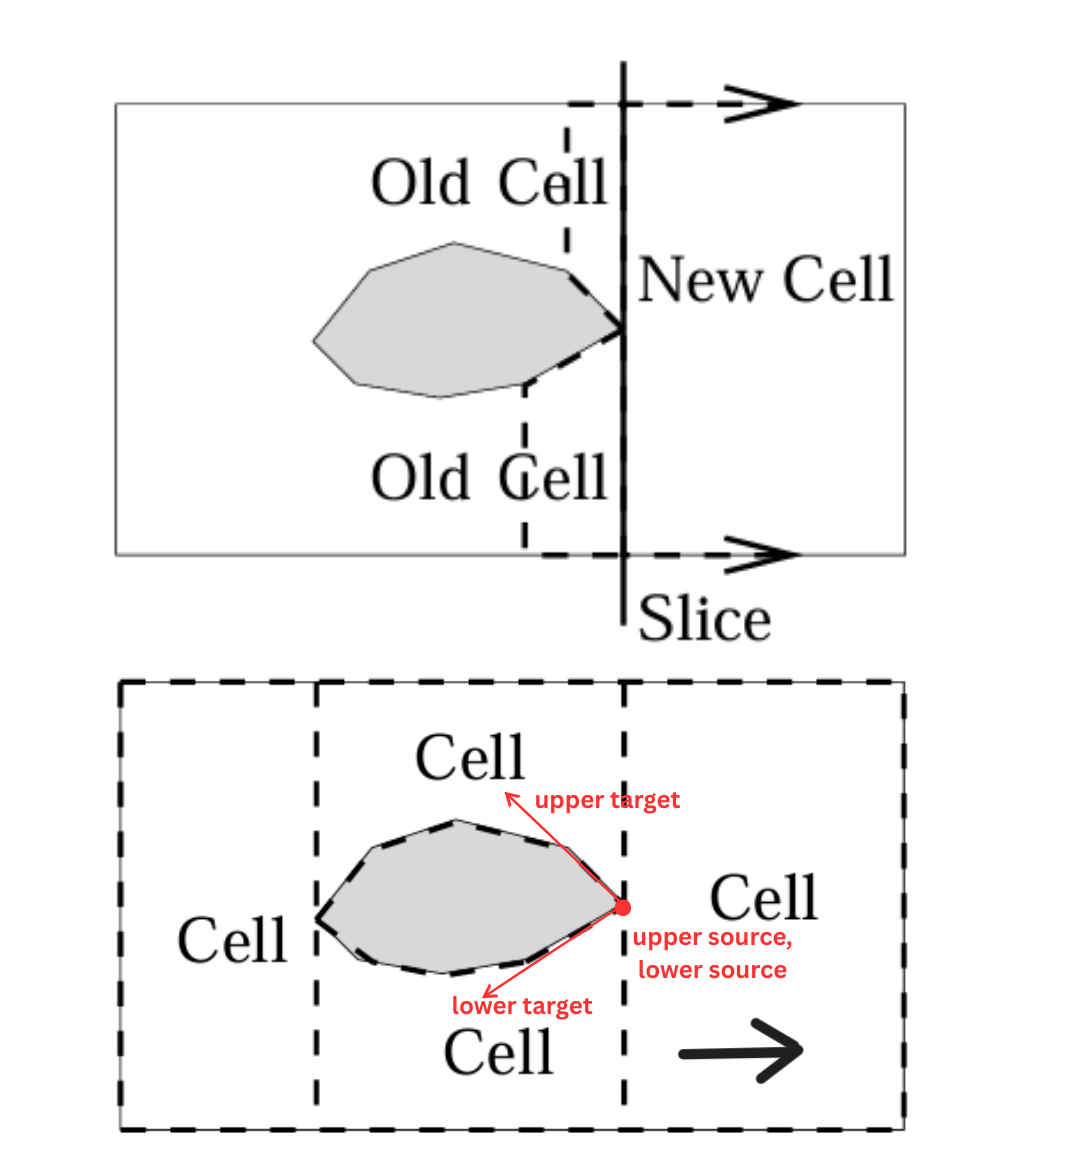
\includegraphics[width=0.6\linewidth]{Included_Images/out_event.png}
        \caption{Boustrophedon Cell Decomposition OUT Event Example \cite{Choset-1997-16422}}
        \label{fig:out_event}
        \end{figure}
\end{itemize}
After the decomposition phase, the algorithm visits the resulting adjacent
cells, typically using a Depth-First Search (DFS) strategy. To guarantee
complete coverage, a backtracking mechanism is utilized to ensure all connected
cells are visited. When visiting each cell, the algorithm generates a sweeping
path based on the given parameters, such as the sweeping direction and sweep
distance. The sweeping direction can be performed horizontally or vertically,
while the sweep angle can be aligned with the polygon's edges. The sweep
distance defines the separation between parallel tracks. Figure
\ref{fig:sweep_parameters} illustrates boustrophedon path in each cell. 
\begin{figure}[H]
    \centering
    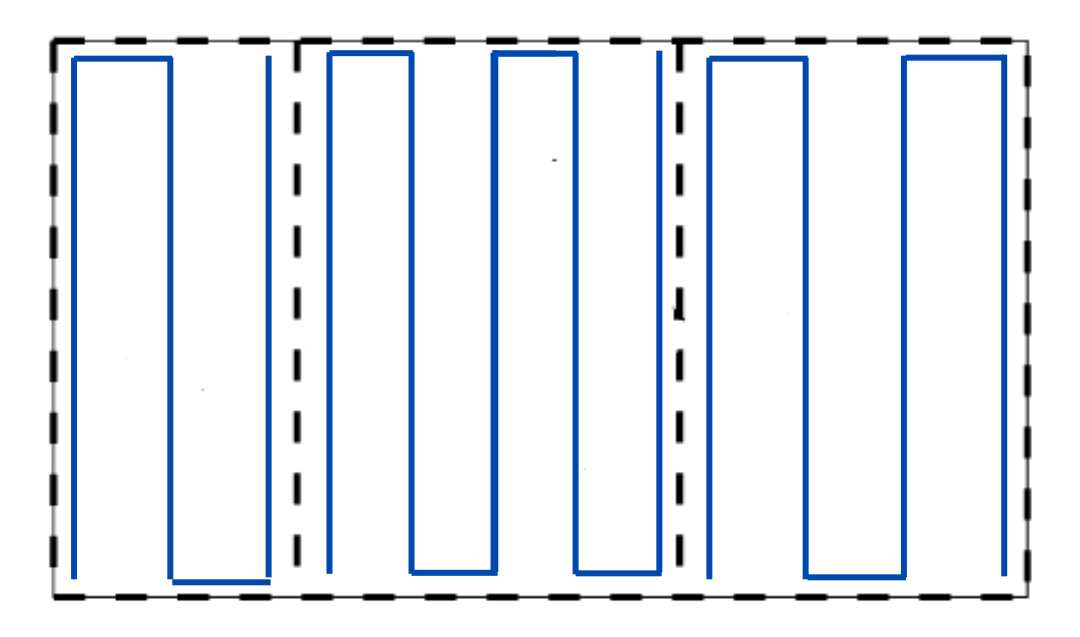
\includegraphics[width=0.4\linewidth]{Included_Images/sweep_parameters.png}
    \caption{Boustrophedon Cell Decomposition Sweeping \cite{Choset-1997-16422}}
    \label{fig:sweep_parameters}
\end{figure}

The practical implications of the algorithm's use are shown in the experiment
setup section, and the detailed results of the Boustrophedon Cell Decomposition
algorithm are discussed in the results and discussion section. 

\subsubsection{Image Processing}
To execute the waypoint-based navigation and coverage path planning, image
processing was used to identify potential vegetation areas in a satellite imagery. The maps were
obtained using QGroundControl \cite{QGroundControl_PlanView} software from
satellite imagery and then imported into an image processing pipeline. The
pipeline can be described in the following steps:

\begin{enumerate}
    \item Converting the satellite imagery to grayscale images.
    \item Using HSV (Hue, Saturation, Value) color space conversion and RGB
    Conversion to identify greenery, and NDVI Index to measure vegetation
    health. The images are categorized into three vegetation types: Dense tree
    canopy, grassland and short vegetation, and cropland and agricultural fields.
    \item Applying edge detection such as canny detection \cite{ding2001canny} to identify buildings and non vegetation areas.
    \item Plotting the series of processed images as occupancy grid maps.
\end{enumerate}

Figure \ref{fig:dense_canopy_map} is an example of processed occupancy grid maps for a dense canopy vegetation:
\begin{figure}[H]
    \centering
    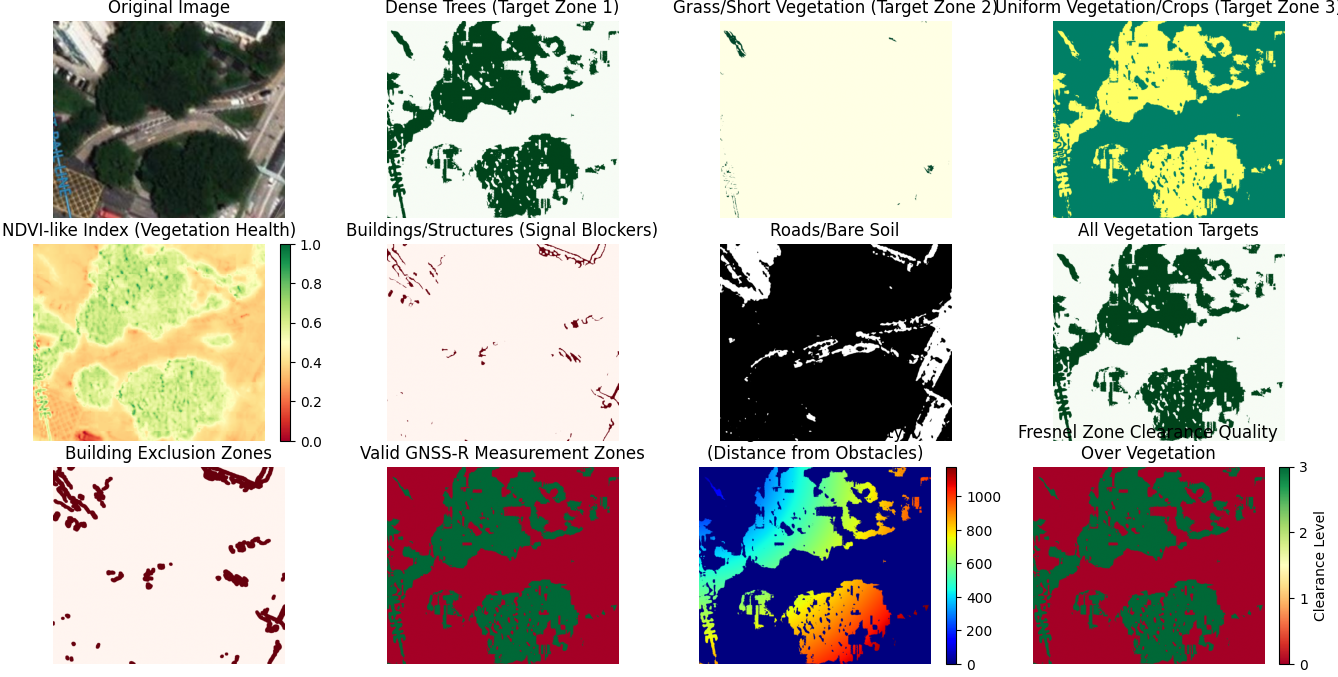
\includegraphics[width=0.9\linewidth]{Included_Images/densecanopy_map.png}
    \caption{Processed Occupancy Grid Map for Dense Canopy Vegetation}
    \label{fig:dense_canopy_map}
\end{figure}

\paragraph{Normalized Difference Vegetation Index} ~\\
The Normalized Difference Vegetation Index (NDVI) is a vegetation index that
measures the difference between near-infrared light and red light. This provides
the difference between signals reflected by vegetation and signals
absorbed by vegetation \cite{GISGeography_NDVI}. Below is the equation to
calculate NDVI:
\begin{equation}
    \text{NDVI} = \frac{\text{NIR} - \text{Red}}{\text{NIR} + \text{Red}}
    \label{eq:ndvi}
\end{equation}
The Normalized Difference Vegetation Index is calculated using Equation
\ref{eq:ndvi}, where \text{NIR} represents the near-infrared band and \text{Red}
represents the red visible light band. 

If vegetation is healthy, it reflects more near-infrared and green light
(associated with chlorophyll) while absorbing more red and blue light.
Therefore, this image processing pipeline enables filtering and identifying
greenery while categorizing vegetation into different types based on hue,
saturation, and intensity characteristics. 

However, in practical applications, identifying vegetation solely from satellite
imagery is insufficient. To determine potential vegetation regions, it is also
necessary to account for the GNSS signal reflection areas, known as the Fresnel
zones (see Section \ref{sec:first_fresnel_zone_calculation}). These areas define
the ellipsoidal detection region where reflected satellite signals can be
captured. Hence, the vegetation analysis is further constrained by the spatial
extent of these Fresnel zones to identify potential areas suitable for GNSS
reflectometry-based sensing.

\subsubsection{Path planning workflow} 
\paragraph{Fresnel Zone Identification} ~\\
To determine the Fresnel zone locations, NASA Broadcast Ephemeris Data Product
\cite{NASA_BroadcastEphemeris} is utilized for a specified geographic location
and time instance. The MATLAB simulation framework developed in this study
computes and visualizes the Fresnel zones for a desired latitude, longitude, and
time instance. The generated Fresnel zones are represented as ellipsoids
corresponding to the GNSS signal reflection areas, along with their respective
center coordinates. These center locations are subsequently used as reference
points for determining the detection area and survey planning.  Figure
\ref{fig:fresnel_zone_identification} shows the Fresnel zones plotted at Mount
Davis Park in Hong Kong on 2026-03-26 at 12:00:00.
\begin{figure}[H]
    \centering
    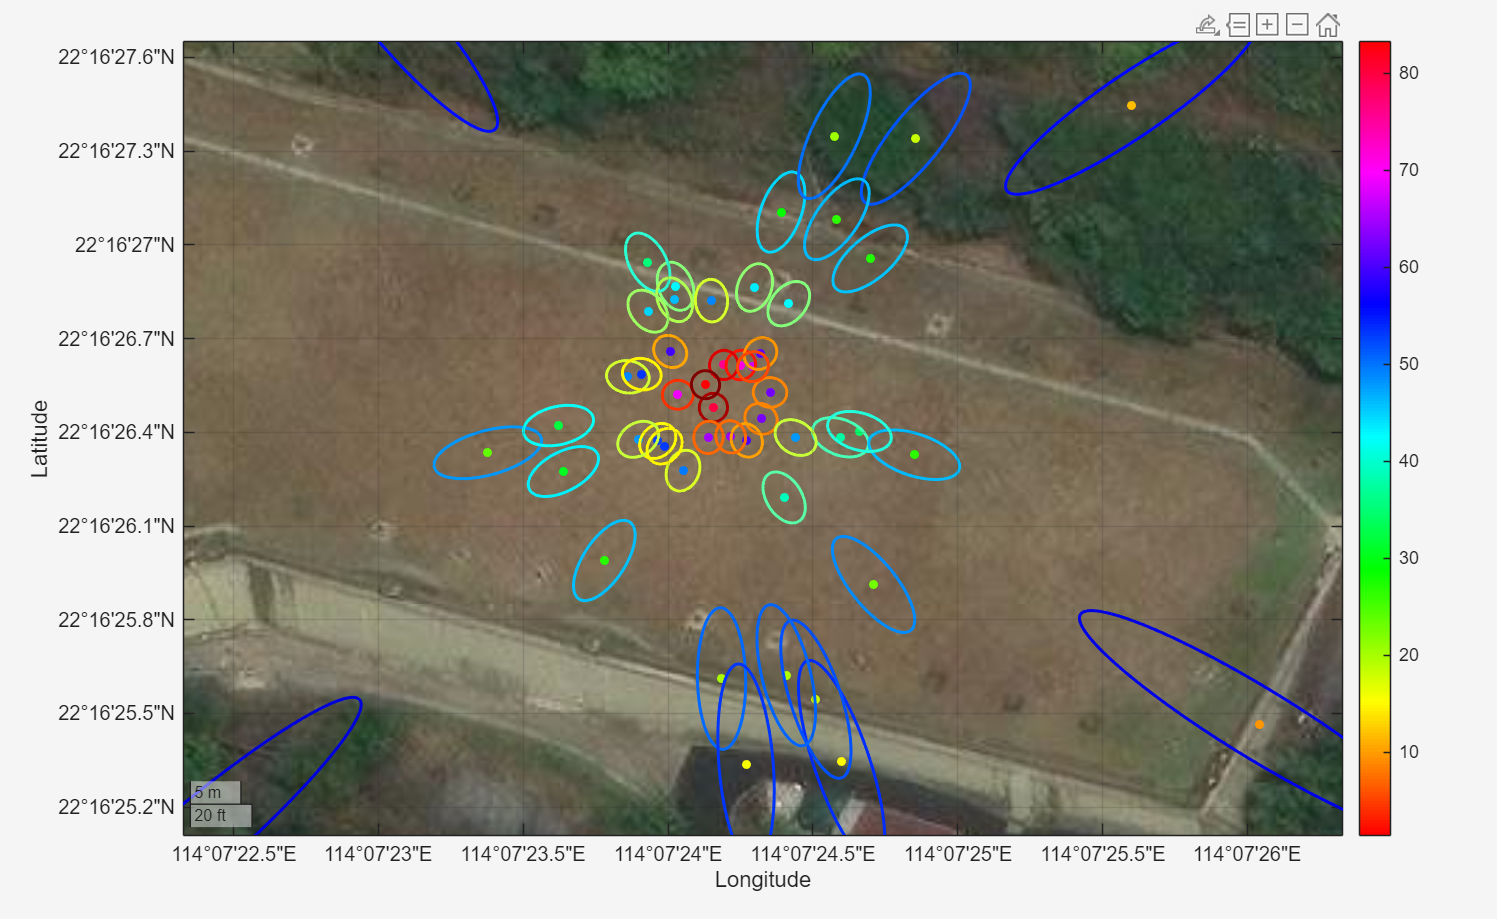
\includegraphics[width=0.75\textwidth]{Included_Images/fresnel_zone_identification.png}
    \caption{Fresnel Zone Identification}
    \label{fig:fresnel_zone_identification}
\end{figure}

However, these Fresnel zones exhibit irregular geometries and complex spatial
boundaries, making it difficult to cover the area of interest. Therefore, a path
planning framework is required to cluster and organize groups of Fresnel zones
into detectable regions that can be effectively covered by the UAV platform
during the survey mission. 

The proposed path planning workflow (Figure \ref{fig:path_planning_workflow}) consists of the following stages:
\begin{enumerate}
    \item Launching the interactive path planner and importing the simulated Fresnel zone locations. 
    \item Performing automatic clustering of Fresnel zones using a nearest-neighbor distance-based algorithm. 
    \item Determining the region of interest (ROI) by extracting the boundary of the generated detection area. 
    \item Computing the required sweeping distance for coverage path planning. 
    \item Configuring and deploying the final survey mission through the ground control system.
\end{enumerate}
\begin{figure}[H]
    \centering
    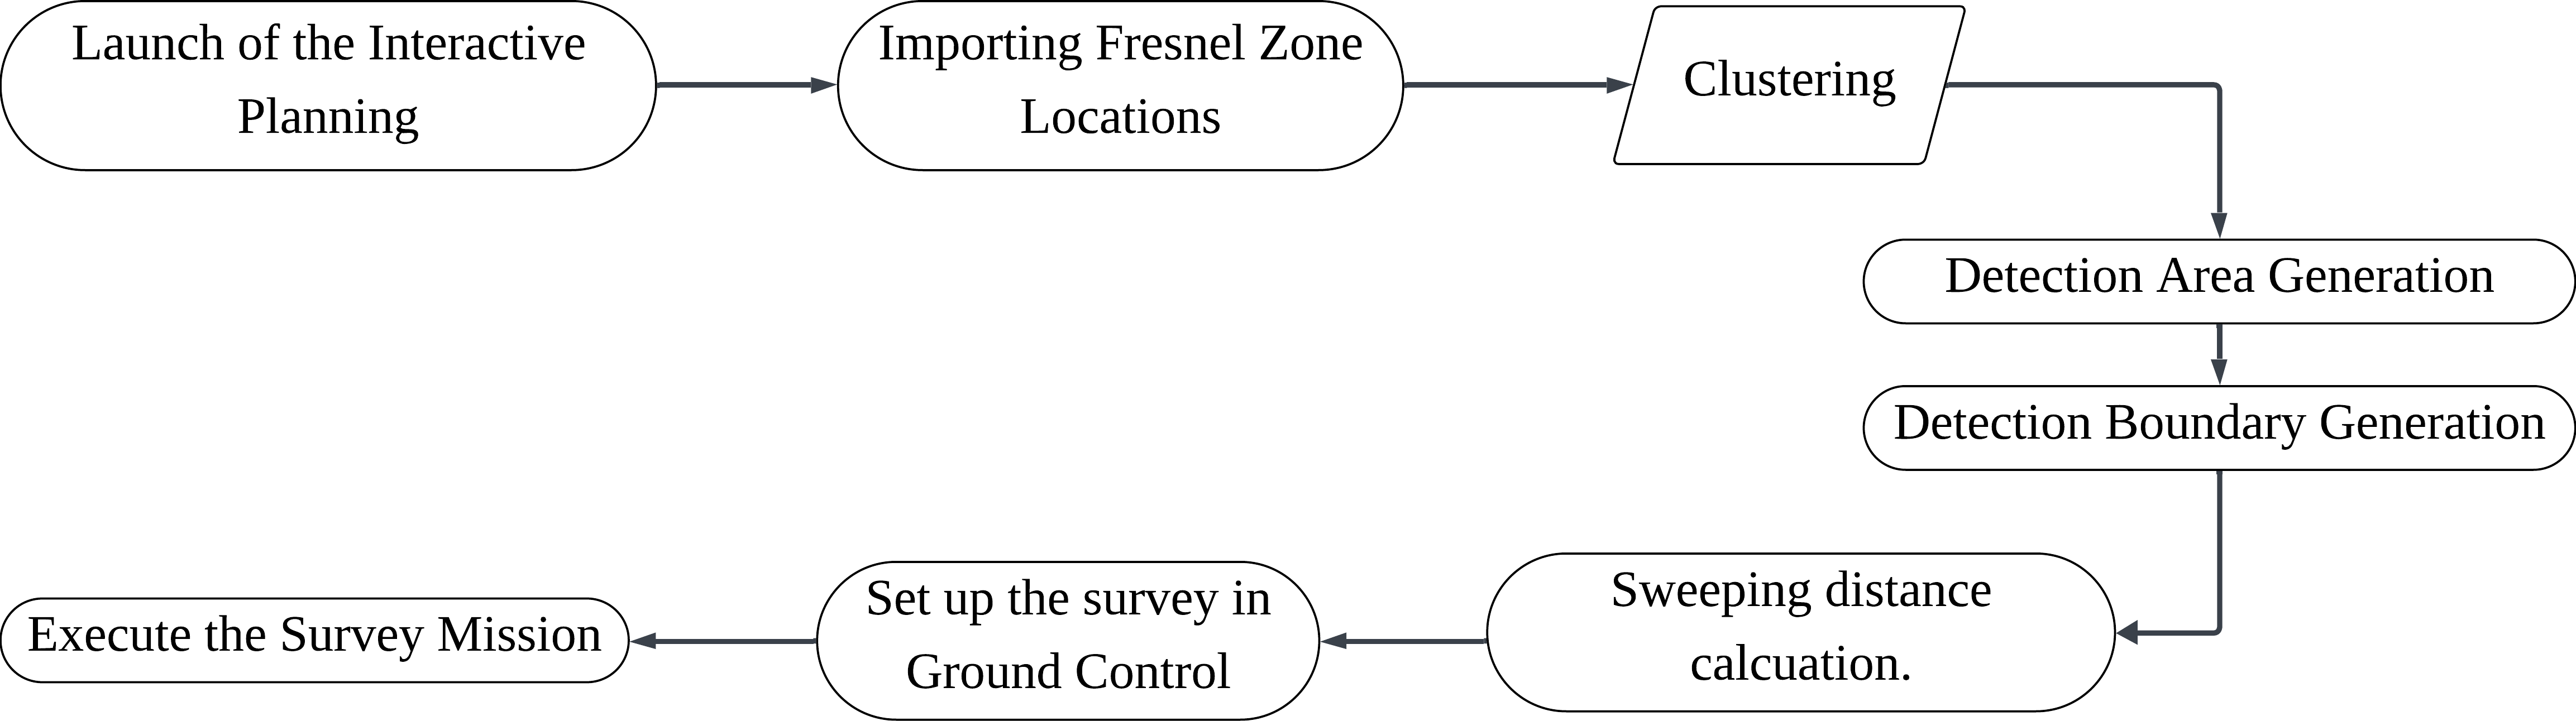
\includegraphics[width=\textwidth]{Included_Images/pathplanning_workflow.png}
    \caption{Path Planning Workflow}
    \label{fig:path_planning_workflow}
\end{figure}

\paragraph{Fresnel Zone Clustering} ~\\
In this system, automatic clustering of Fresnel zones is performed using a
nearest-neighbor distance-based clustering method. Initially, all simulated
Fresnel zone locations, including their corresponding center coordinates, are
imported into the interactive path planner. A global center is then computed to
represent the overall spatial distribution of the Fresnel zones within the
survey area. Subsequently, pairwise distances between all Fresnel zones are
calculated, and a distance distribution is generated to analyze their spatial
relationships. 

Based on this distribution, a clustering threshold is defined to identify
neighboring Fresnel zones that are closely aligned. In this study, the threshold
is selected to include approximately the closest 40\% of Fresnel zones, allowing
closer adjacent zones to be grouped into clusters. If multiple clusters are
identified, the algorithm selects the cluster that is closest to the global
center. The selected cluster is then designated as the primary region of
interest, also known as the detection area. Figure \ref{fig:clustering_algo}
illustrates the flowchart of the neighbor distance clustering algorithm.
\begin{figure}[H]
    \centering
    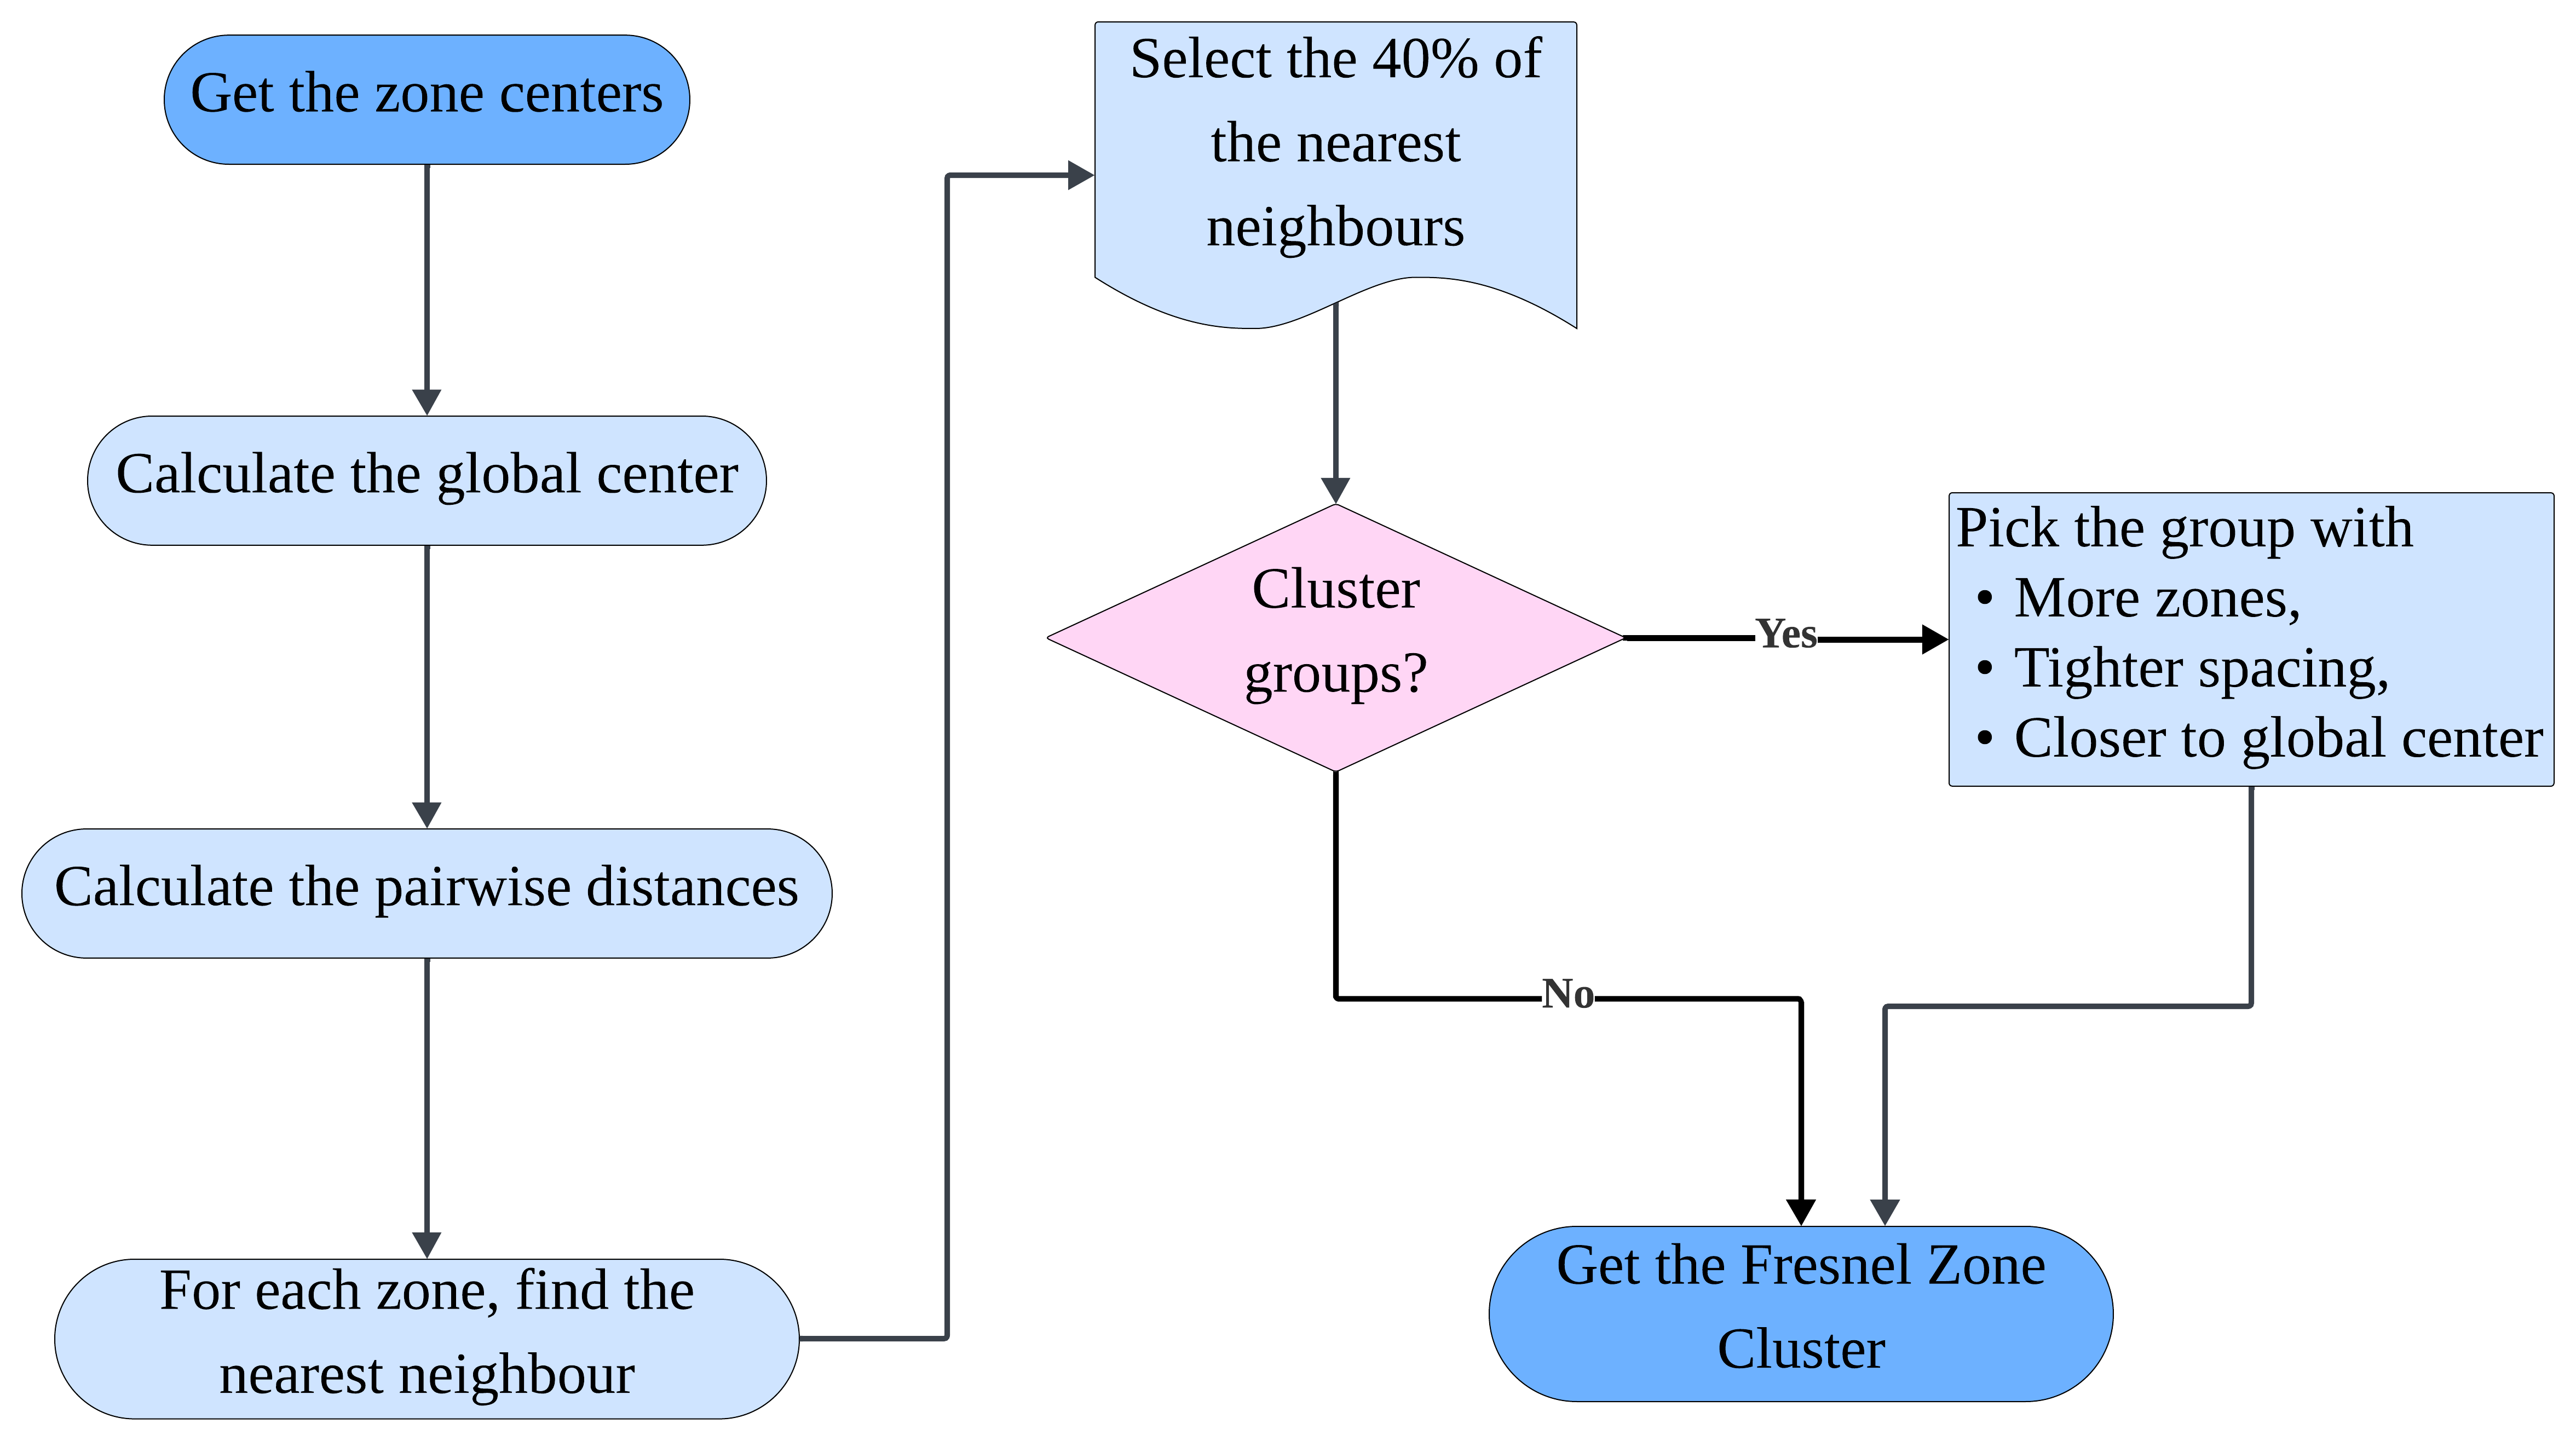
\includegraphics[width=0.8\textwidth]{Included_Images/clustering_algo.png}
    \caption{Neighbor Distance Clustering Algorithm}
    \label{fig:clustering_algo}
\end{figure}
Figure \ref{fig:fresnel_cluster} shows a selected Fresnel zone cluster
for experiment conducted at Mount Davis Park in Hong Kong. 
\begin{figure}[H]
    \centering
    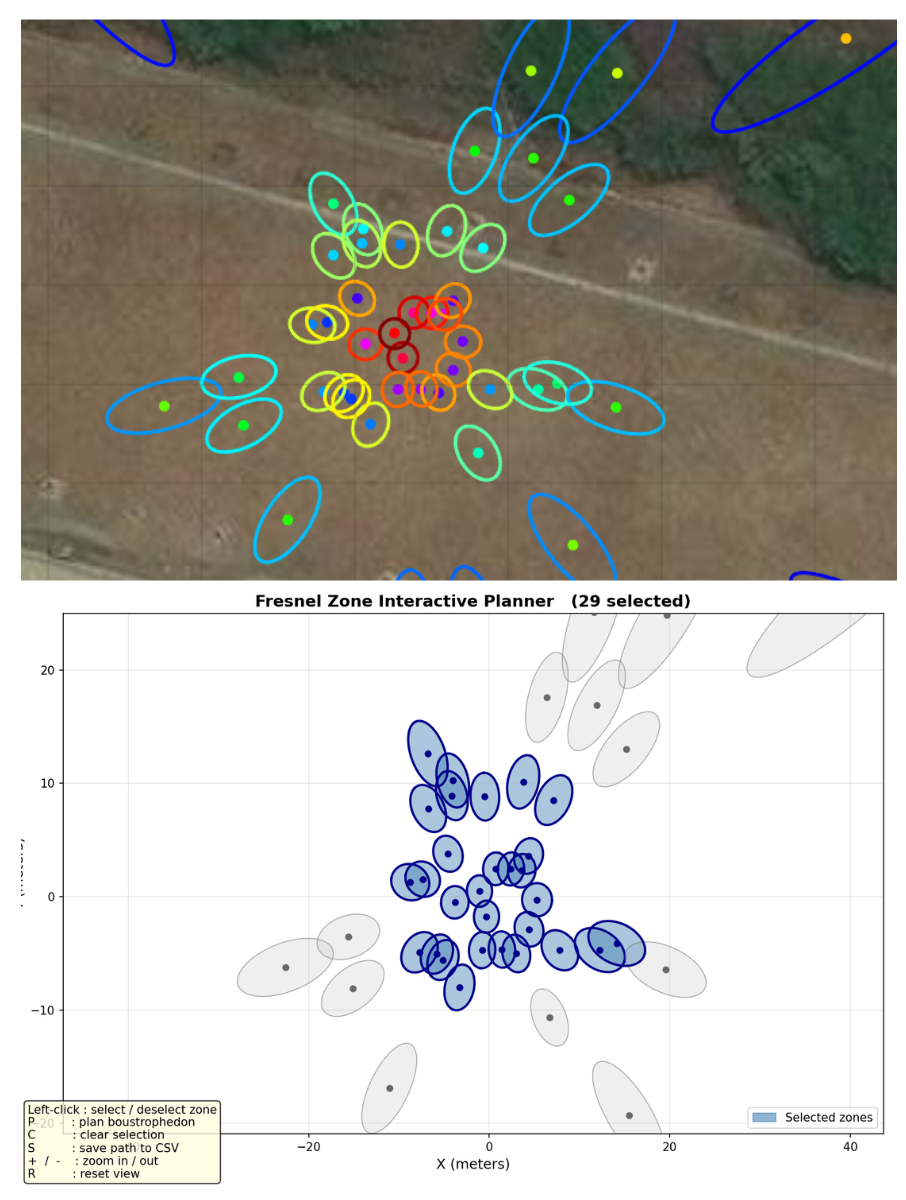
\includegraphics[width=0.6\textwidth]{Included_Images/fresnel_cluster.png}
    \caption{Fresnel Zone Cluster}
    \label{fig:fresnel_cluster}
\end{figure}

\paragraph{Fresnel Cluster Boundary Determination} ~\\
To address the complex geometry of the selected Fresnel zone cluster, it is
necessary to bound the detection area with a simplified shape. To determine the
region of interest (ROI), the selected Fresnel zones must be enclosed
within an appropriate boundary.
In this study, three boundary geometries are considered: square, circular, and
triangular enclosures, as shown in Figure \ref{fig:boundries}. For each geometry, the algorithm generates an enclosure
based on the spatial coordinates of the selected Fresnel zone ellipsoids,
ensuring that all ellipsoids are fully contained within the boundary. Once the
three areas are established, their enclosed areas are computed to evaluate the
most suitable detection region.

\begin{figure}[H]
    \centering
    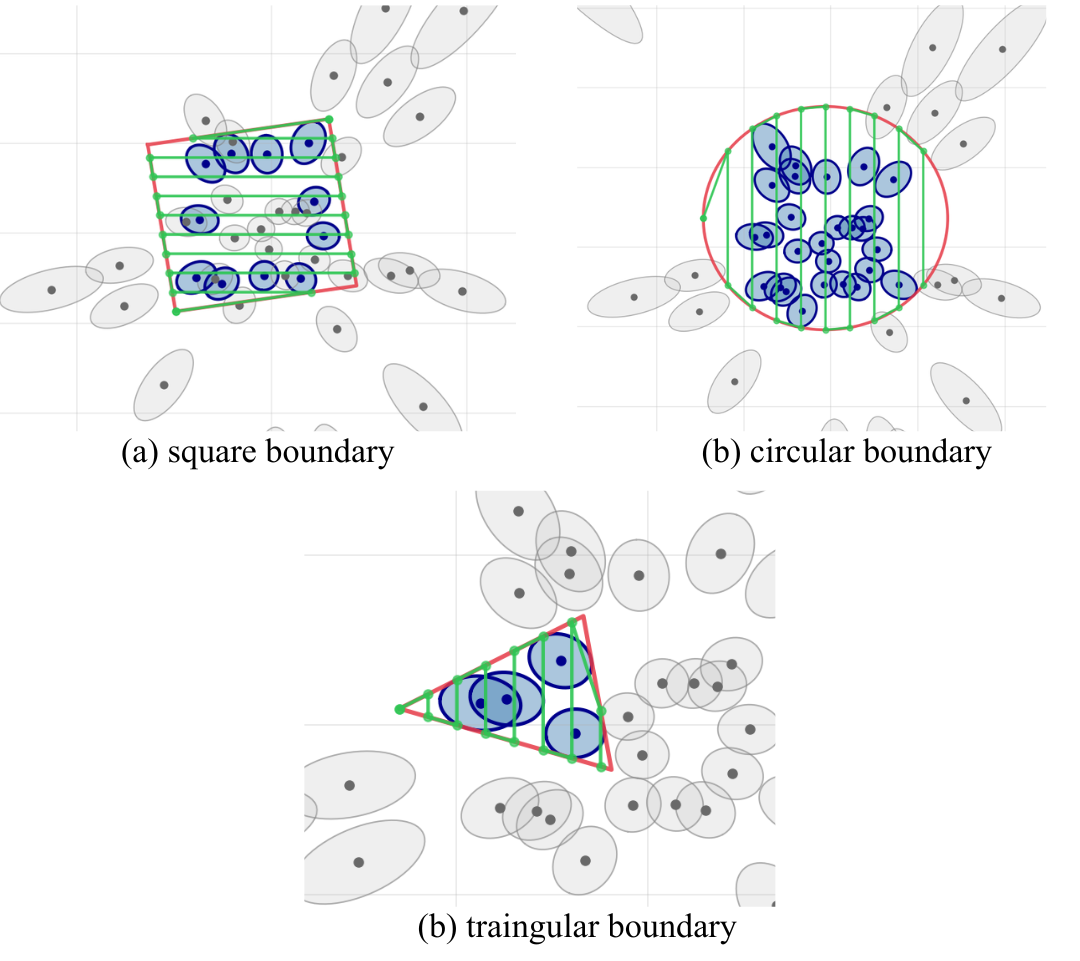
\includegraphics[width=\textwidth]{Included_Images/boundries.png}
    \caption{Fresnel cluster boundary determination}
    \label{fig:boundries}
\end{figure}

To optimize the area of interest, the algorithm calculates the
\textit{coverage ratio} for each shape. The coverage ratio is defined as the ratio
between the total area occupied by the selected Fresnel zones and the area of
the corresponding enclosure, as shown in Equation \ref{eq:coverage_ratio}:

\begin{equation}
    \text{Coverage Ratio} = \frac{A_{\text{Fresnel Zones}}}{A_{\text{Enclosure}}}
    \label{eq:coverage_ratio}
\end{equation}

Where $A_{\text{Fresnel Zones}}$ represents the total area covered by the
selected Fresnel zone ellipsoids, and $A_{\text{Enclosure}}$ denotes the area
of the generated boundary.

In addition, the area without Fresnel zones (empty area) within the enclosure can be calculated as:
\begin{equation}
    A_{\text{Empty}} = A_{\text{Enclosure}} - A_{\text{Fresnel Zones}}
    \label{eq:empty_area}
\end{equation}

The optimal detection area is selected by choosing the enclosure with the
highest coverage ratio, corresponding to the smallest empty area. This ensures
that the final detection area maximizes coverage efficiency and obtains strong
GNSS reflected signals.             

\paragraph{Detection Area Evaluation} ~\\
For coverage path planning, it is necessary to define the sweeping distance,
which represents the spacing between adjacent sweeps during the survey mission.
In this system, the sweeping distance is determined based on the detection area
obtained from the previous boundary determination step. Figure \ref{fig:d_sweep}
illustrates the sweeping distance in coverage path planning. 

\begin{figure}[H]
    \centering
    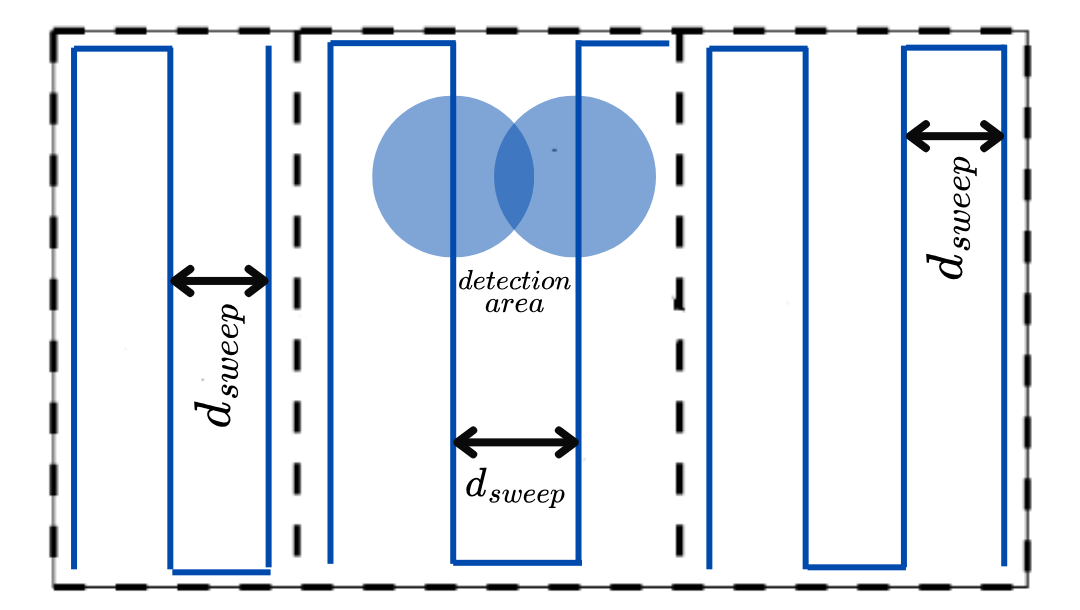
\includegraphics[width=0.6\textwidth]{Included_Images/d_sweep.png}
    \caption{Sweeping distance in coverage path planning}
    \label{fig:d_sweep}
\end{figure}
To calculate the optimal distance between flight lines, $d_{\text{sweep}}$, the
area of the selected detection region ($A$) and the geometric shape of the
detection boundary are taken into account, as shown in Equation
\ref{eq:sweep_distance} \cite{DeWitt_2000}:
\begin{equation}
    d_{\text{sweep}} = (1-o)\cdot k \cdot \sqrt{A}
    \label{eq:sweep_distance}
\end{equation}
where:
\begin{itemize}
    \item $d_{\text{sweep}}$ :Spacing parameter in QGroundControl
    \item $A$ : Area of the selected detection boundary
    \item $k$ : Geometric shape factor
    \item $o$ : Overlap percentage between adjacent sweeps
\end{itemize}
The sweeping distance is calculated according to Equation
\ref{eq:sweep_distance}, where the resulting gap varies proportionally with both
the area and geometry of the detection region. Figure \ref{fig:d_sweep} shows
how detection area is used in coverage path planning with corresponding
overlapping. To ensure sufficient sensing coverage between adjacent sweeps, a
constant overlap factor of 20\% is applied in real-world experiments.

Table \ref{tab:detection_area_comparison} presents a comparison of different
detection areas with a triangular boundary. In this analysis,
the overall survey area is considered to be constant. It can be observed that smaller
detection areas result in shorter sweeping distances, whereas larger detection
areas produce proportionally larger sweeping distances. However, in terms of
energy consumption, smaller detection areas have a higher energy consumption
since more sweeps are needed to achieve full coverage. In contrast, larger
detection areas require fewer sweeps, resulting in lower energy consumption. The
energy consumption values presented are estimated based on the
battery capacity and operational characteristics of the Holybro X650 drone
platform. Based on these results, a mid-range detection area is the most
practical choice, as it balances operational efficiency, energy consumption, and
coverage ratio. 
\begin{table}[H]
    \centering
    \caption{Comparison of detection areas and sweeping distance}
    \label{tab:detection_area_comparison}
    \renewcommand{\arraystretch}{2.0}
    
    \resizebox{\textwidth}{!}{
    \begin{tabular}{|p{5cm}|c|c|m{6cm}|}
    \hline
    \textbf{Detection Area} & \textbf{Sweeping Distance (m)} & \textbf{Energy Consumed (J)} & \textbf{Comparison} \\
    \hline
    
    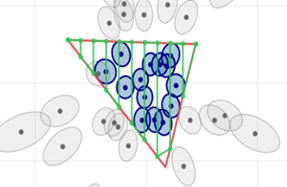
\includegraphics[width=5cm]{Included_Images/detection_area_1.png}\newline
    89.00m$^2$
    & 14.33
    & 4000
    & High coverage ratio, High energy consumption.
    \\
    \hline
    
    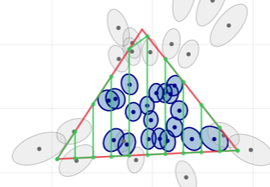
\includegraphics[width=5cm]{Included_Images/detection_area_2.png}\newline
    140.00m$^2$
    & 17.89
    & 3190
    & Provides a balanced efficiency with a higher coverage ratio. In practice, this is the optimal detection area. \\
    \hline
    
    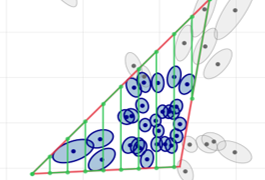
\includegraphics[width=5cm]{Included_Images/detection_area_3.png}\newline
    264.00m$^2$
    & 24.70
    & 2322
    & Low coverage ratio, Low energy consumption.\\
    \hline
    
    \end{tabular}
    }
\end{table}
To summarize, this path planning workflow provides optimal detection and survey
areas for the UAV to fly above vegetation and collect reflected GNSS signals and
dynamic LiDAR data to support SLAM. 

\subsection{Results and Discussion}
\subsubsection{Waypoint-based Navigation Results}
The results of the waypoint-based navigation can be divided into two platforms,
as test runs were conducted using both a locally developed A* algorithm and
a waypoint navigation in QGroundControl. 

\paragraph{Locally Developed A* Algorithm Results} ~\\
The A* algorithm evaluation results were obtained in various types of
vegetation environments, including dense forests, crop fields, and grasslands.
The images are obtained from the QGroundControl satellite imagery and sent to
the image processing pipeline to identify the potential flying areas. 

Figure \ref{fig:forest_path} shows two different start and end points, and how
the A* algorithm finds the shortest path between them in a dense forest canopy.
Here, the image processing filter is designed to identify darker shades of
green. Therefore, the algorithm fits precisely to predict the paths in the dense
area.
\begin{figure}[H]
    \centering
    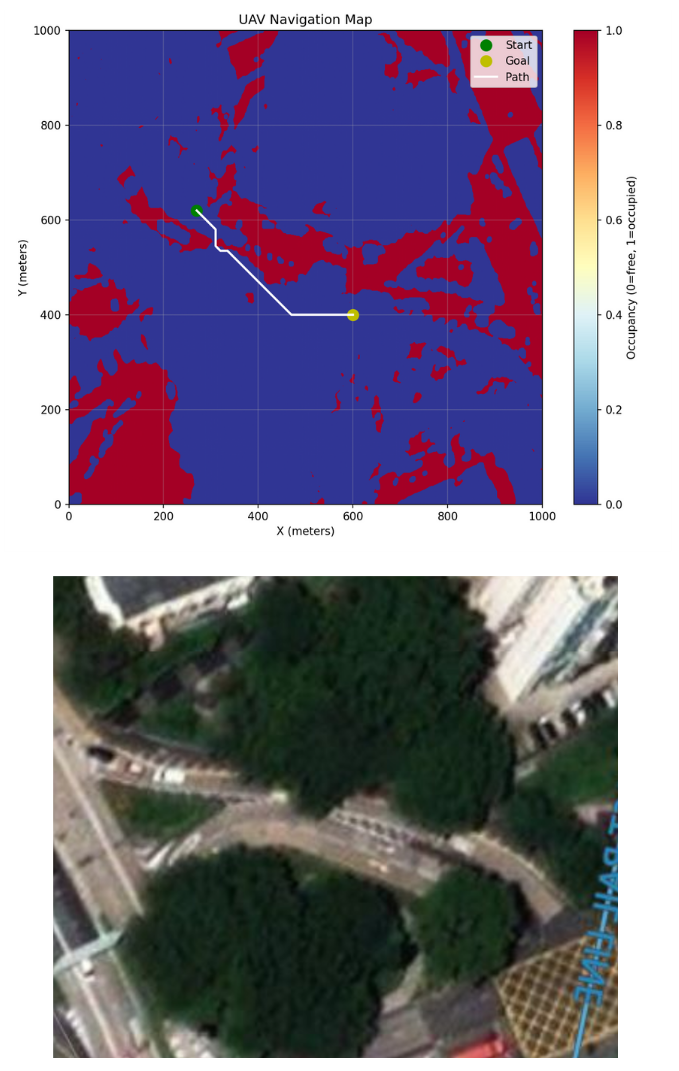
\includegraphics[width=0.6\textwidth]{Included_Images/forest_path.png}
    \caption{A* path planning in dense forest canopy}
    \label{fig:forest_path}
\end{figure}
Similarly, Figure \ref{fig:grassland_path} and Figure \ref{fig:mixed_path} show how
the A* algorithm determines the path to a grassland and to a combination of land
and dense canopy. Since the filter is designed to filter out light shades of
green color, the dense vegetation is considered occupied. Therefore, the
algorithm will avoid converging on paths that lead to dense vegetation. 
\begin{figure}[H]
    \centering
    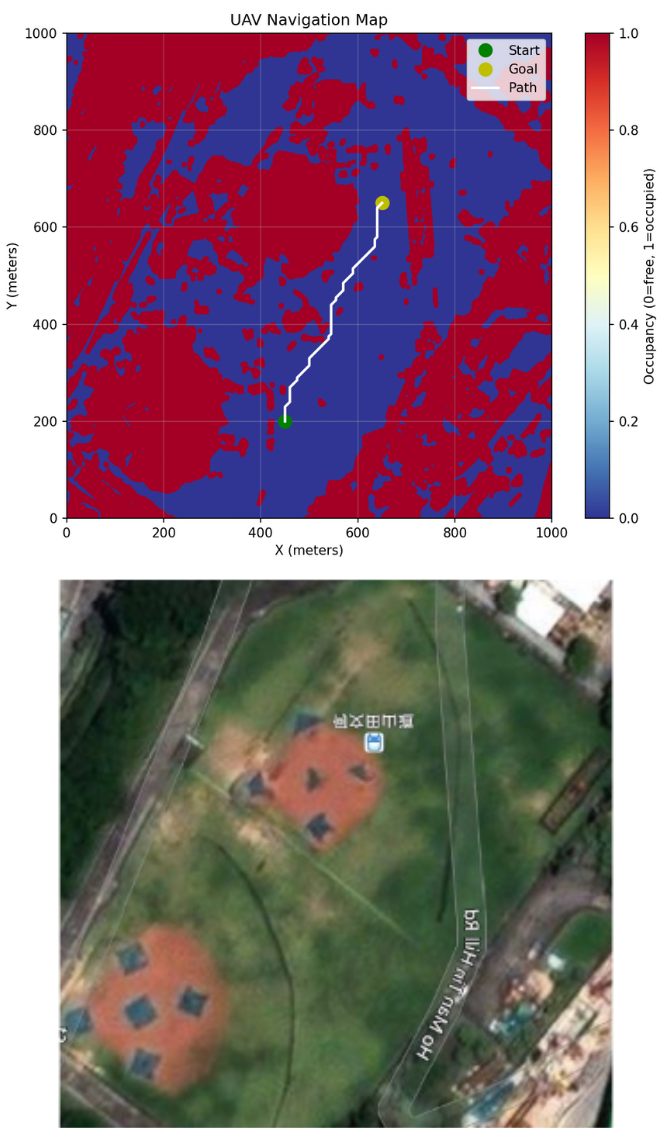
\includegraphics[width=0.8\textwidth]{Included_Images/grassland_path.png}
    \caption{A* path planning in grassland area}
    \label{fig:grassland_path}
\end{figure}
\begin{figure}[H]
    \centering
    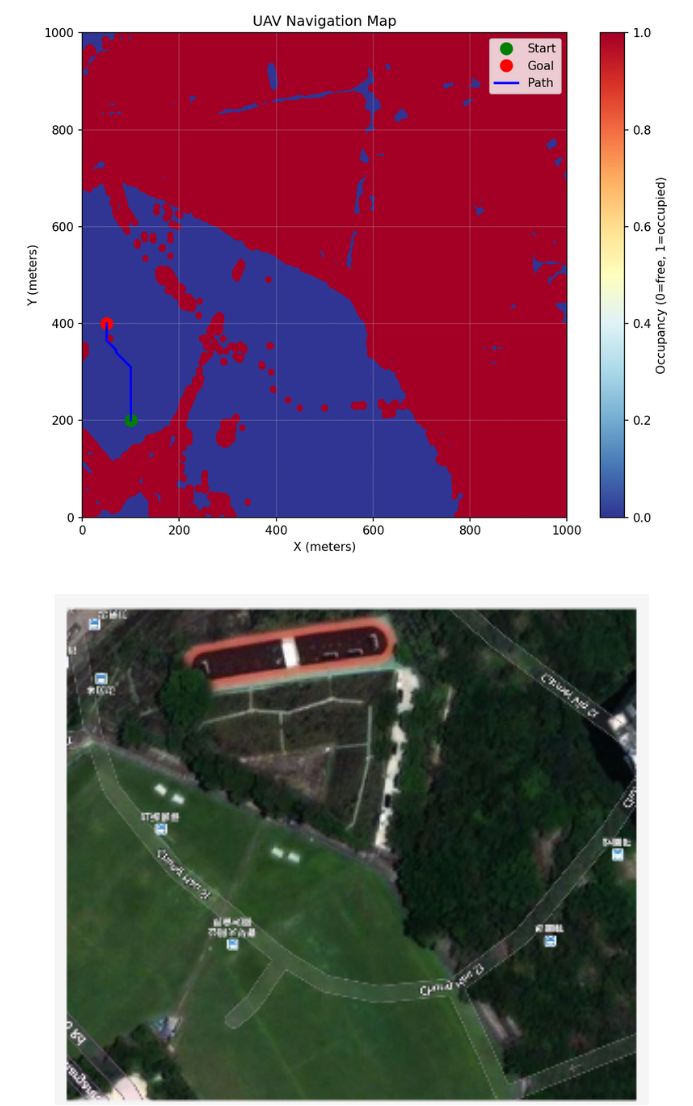
\includegraphics[width=0.8\textwidth]{Included_Images/mixed_path.png}
    \caption{A* path planning in mixed land and dense canopy area}
    \label{fig:mixed_path}
\end{figure}

In order to analyze the dynamic behavior of the locally developed A* algorithm,
simulation studies were conducted in MATLAB. The simulations were implemented
using the MATLAB UAV Simulator \cite{MathWorks_UAV_Delivery}, with the locally developed A* algorithm
integrated into the UAV control pipeline. Figure \ref{fig:control_pipeline}
shows the integration of A* algorithm into the UAV control pipeline, and Figure
\ref{fig:simulation_results} shows UAV flying autonomously in an urban environment.
\begin{figure}[H]
    \centering
    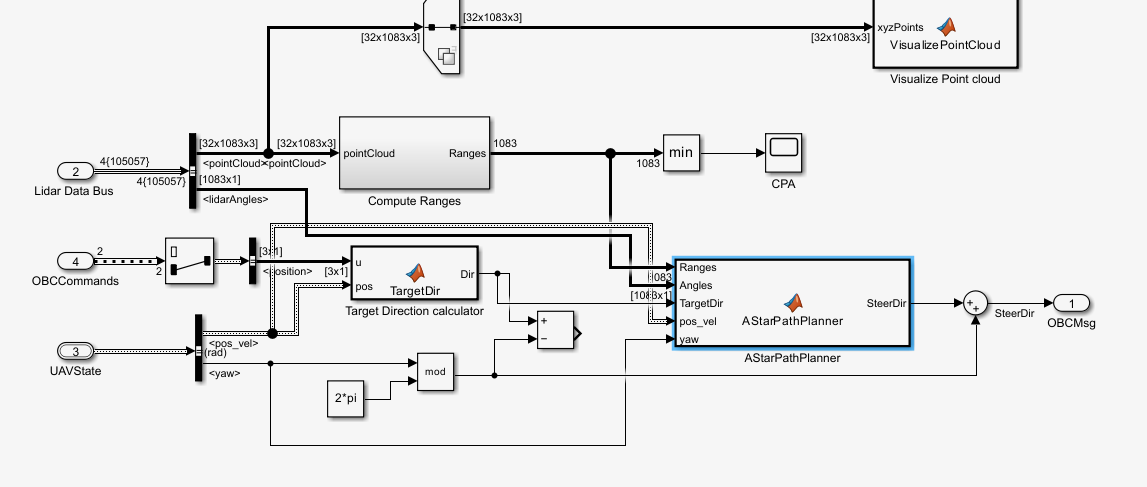
\includegraphics[width=0.9\textwidth]{Included_Images/control_pipeline.png}
    \caption{Integration of A* algorithm into the UAV control pipeline}
    \label{fig:control_pipeline}
\end{figure}
\begin{figure}[H]
    \centering
    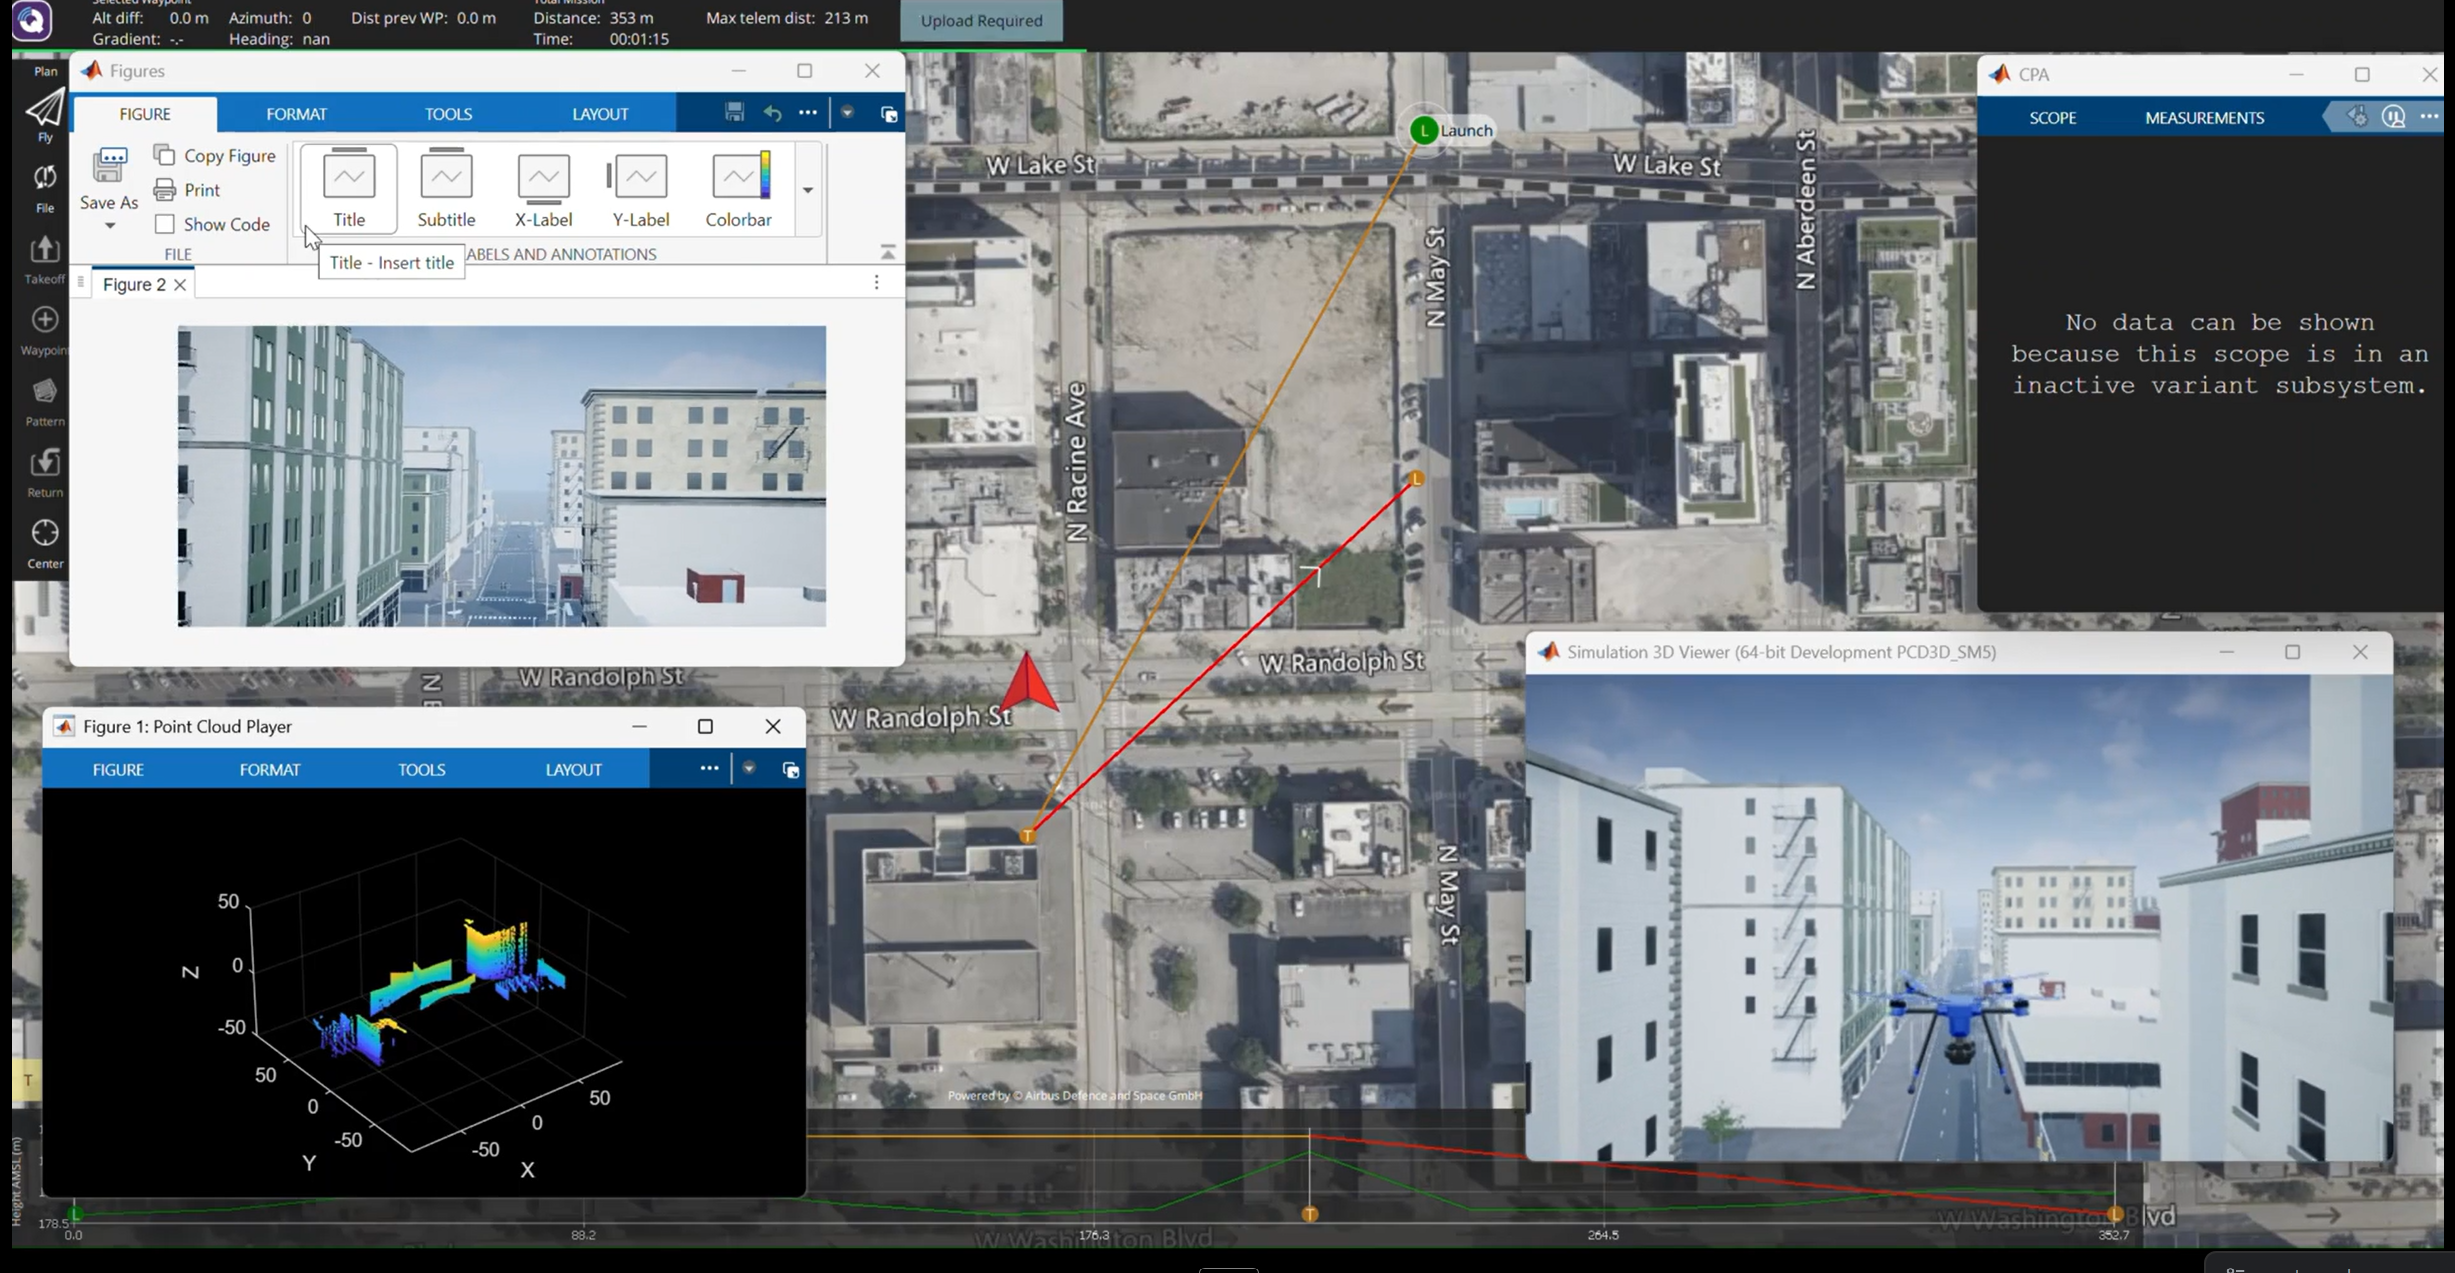
\includegraphics[width=0.8\textwidth]{Included_Images/simulation_results.png}
    \caption{UAV flying autonomously in an urban environment}
    \label{fig:simulation_results}
\end{figure}

\paragraph{QGroundControl Waypoint-based Navigation} ~\\
In QGroundControl, the trajectory is designed by utilizing the parameters such
as waypoints, flying speed, and flying altitude. Then, the plan of waypoints,
also known as the mission, can be uploaded to the Pixhawk flight controller via
telemetry. Figure \ref{fig:qgc_mission} shows the settings and the successful execution of a
mission. 
\begin{figure}[H]
    \centering
    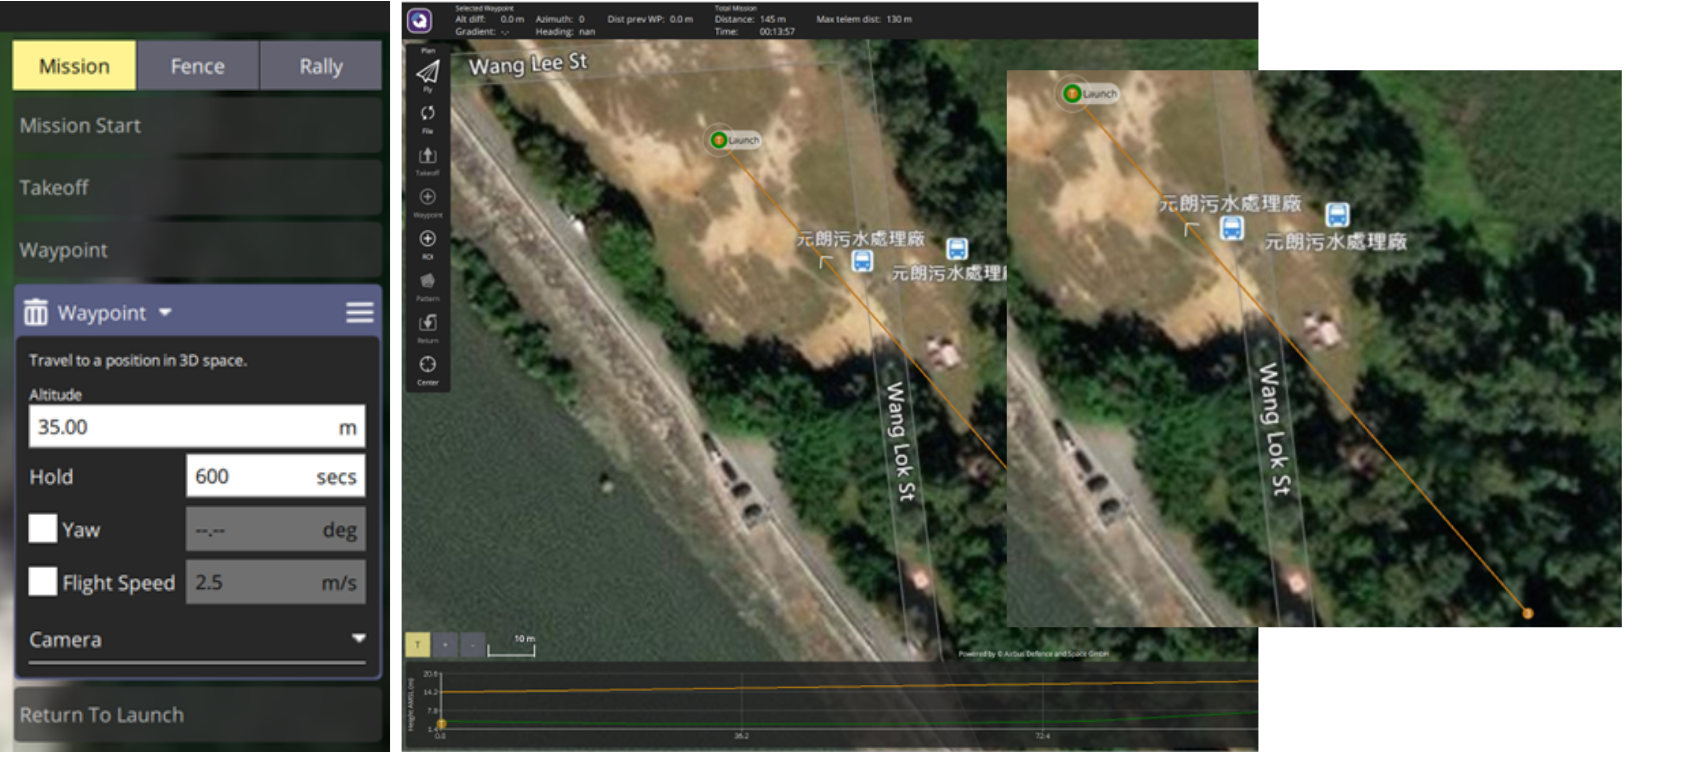
\includegraphics[width=0.8\textwidth]{Included_Images/gqc_mission.png}
    \caption{Waypoint-based navigation mission planning in QGroundControl}
    \label{fig:qgc_mission}
\end{figure}
\subsubsection{Coverage Path Planning Results}
The coverage-based path planning results are divided into three segments: a
locally implemented boustrophedon algorithm, fresnel zone clustering and
detection area generation, and coverage mission planning in QGroundControl.
\paragraph{Boustrophedon Implementation Results} ~\\
The algorithm results were obtained by running the ROS (Robot Operating System) \cite{ROS_website}
package developed by the Autonomous Systems Lab at ETH Zurich \cite{B_hnemann_2021}. The experiments
were conducted in an Ubuntu 22.2 Linux environment. 
At first, the map was specified as a polygon in the graphical user interface.
Once giving the input, the algorithm will determine the coordinates of the
polygon, the sweep distance, and the altitude. An example of result
interpretation for a polygon shown in Figure \ref{fig:cpp_result} is as follows: 
\begin{figure}[H]
    \centering
    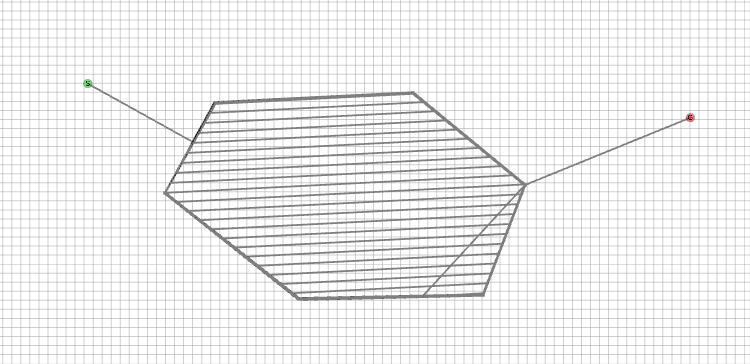
\includegraphics[width=0.6\textwidth]{Included_Images/cpp_result.png}
    \caption{Coverage path planning result interpretation}
    \label{fig:cpp_result}  
\end{figure}

For the Figure \ref{fig:cpp_result}, the polygon is considered to be 3 meters
high in altitude. This simulates a camera or a sensor flying at 3m height with a
field of view. The sweeps are spaced 1.07177m apart to ensure 60 percent overlap
between consecutive passes. The Boustrophedon algorithm divides the polygon
into one cell that can be swept in a back-and-forth pattern. The algorithm
generated 24 possible sweep patterns across the cell. 

Following the initial polygon path planning tests, the system was further
evaluated in an environment containing polygonal obstacles. The simulation
environment is illustrated in Figure \ref{fig:env_obstacles}, in this case,
algorithm detected 7 polygons, with 72 nodes. 
\begin{figure}[H]
    \centering
    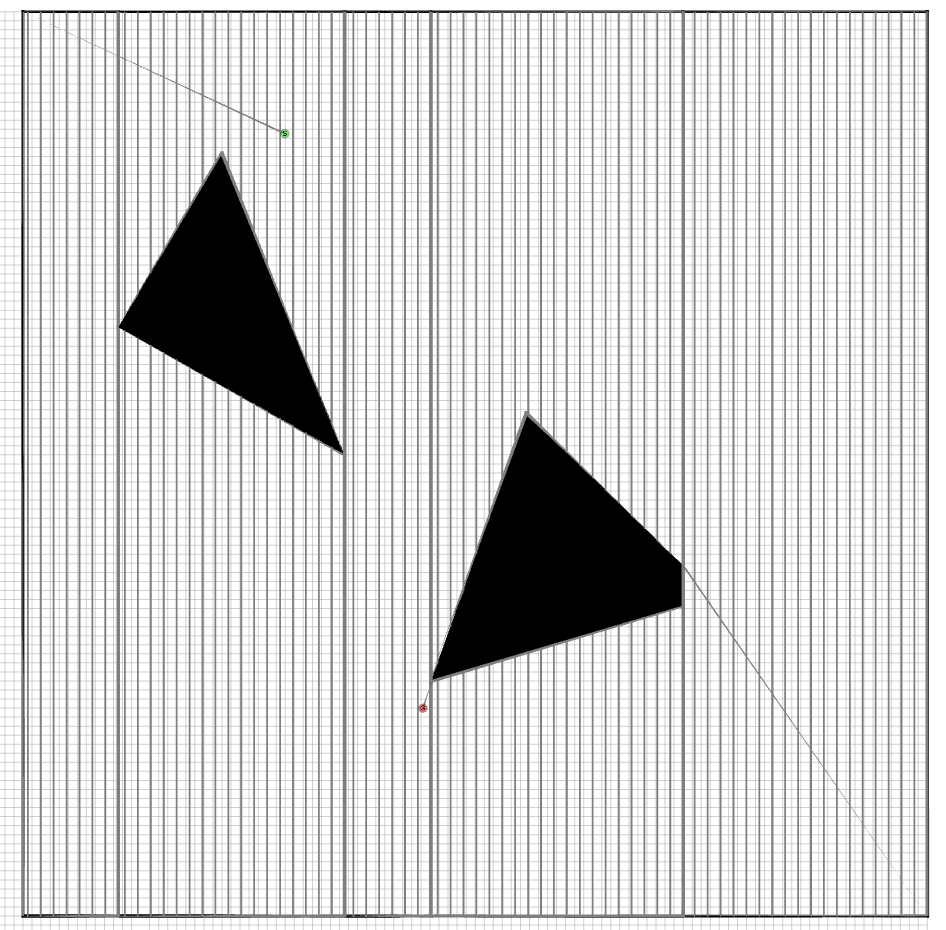
\includegraphics[width=0.6\textwidth]{Included_Images/env_obstacles.png}
    \caption{Coverage path planning environment with obstacles}
    \label{fig:env_obstacles}   
\end{figure}

\paragraph{Fresnel Zone Clustering and Detection Area Generation} ~\\
This section presents the results of the path-planning workflow obtained by
executing the interactive path planner. The interactive path planner is developed
to achieve the optimal detection area and the desired sweeping distance, in
order to obtain the optimal coverage during the survey mission. 

\begin{figure}[H]
    \centering
    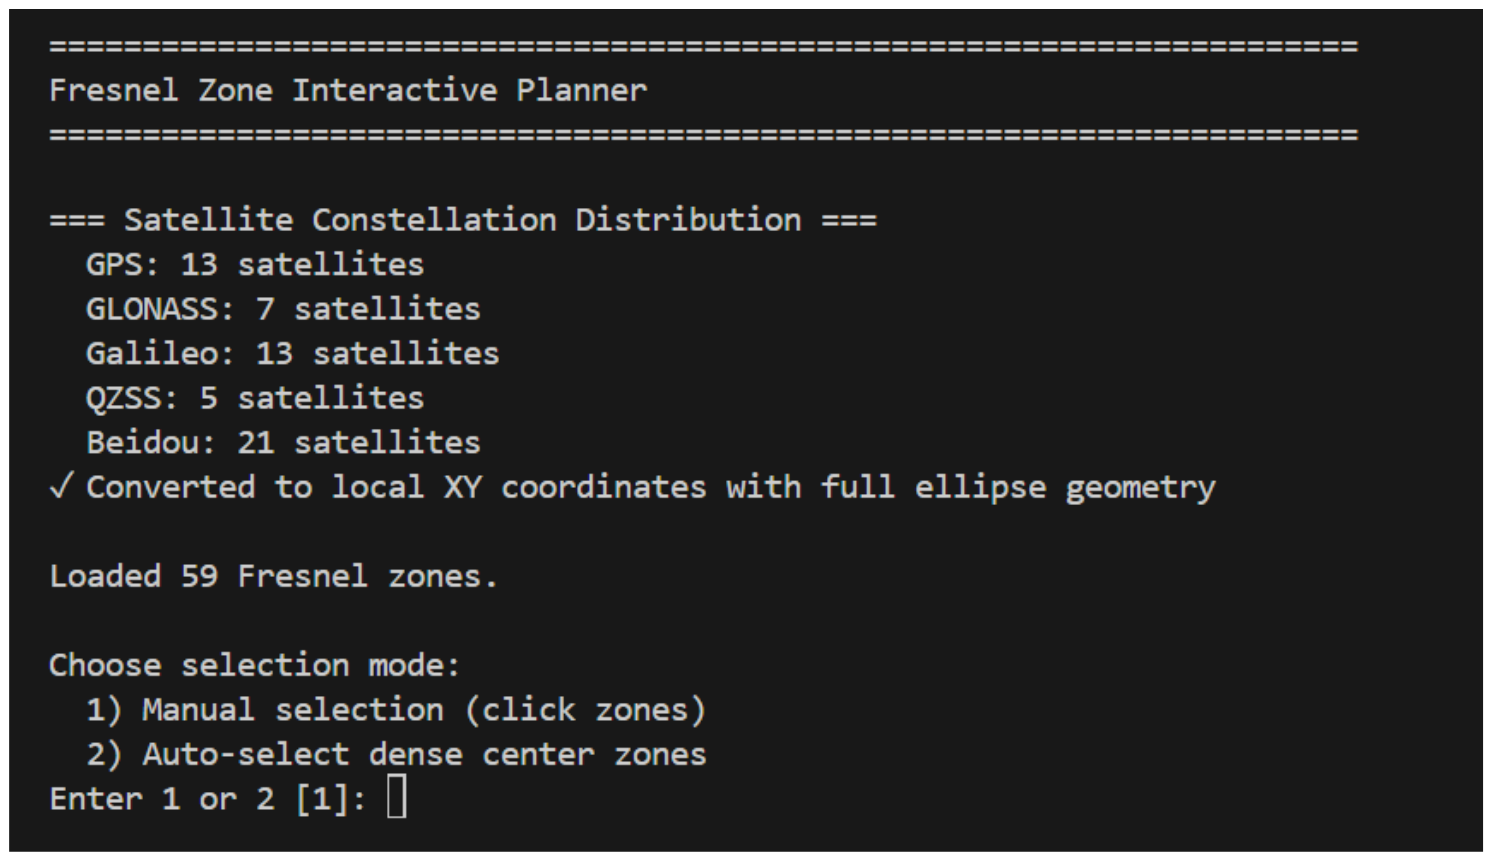
\includegraphics[width=0.8\textwidth]{Included_Images/command_line.png}
    \caption{Command-line output of the path-planning workflow}
    \label{fig:fresnel_zone_clustering}
\end{figure}

\begin{figure}[H]
    \centering
    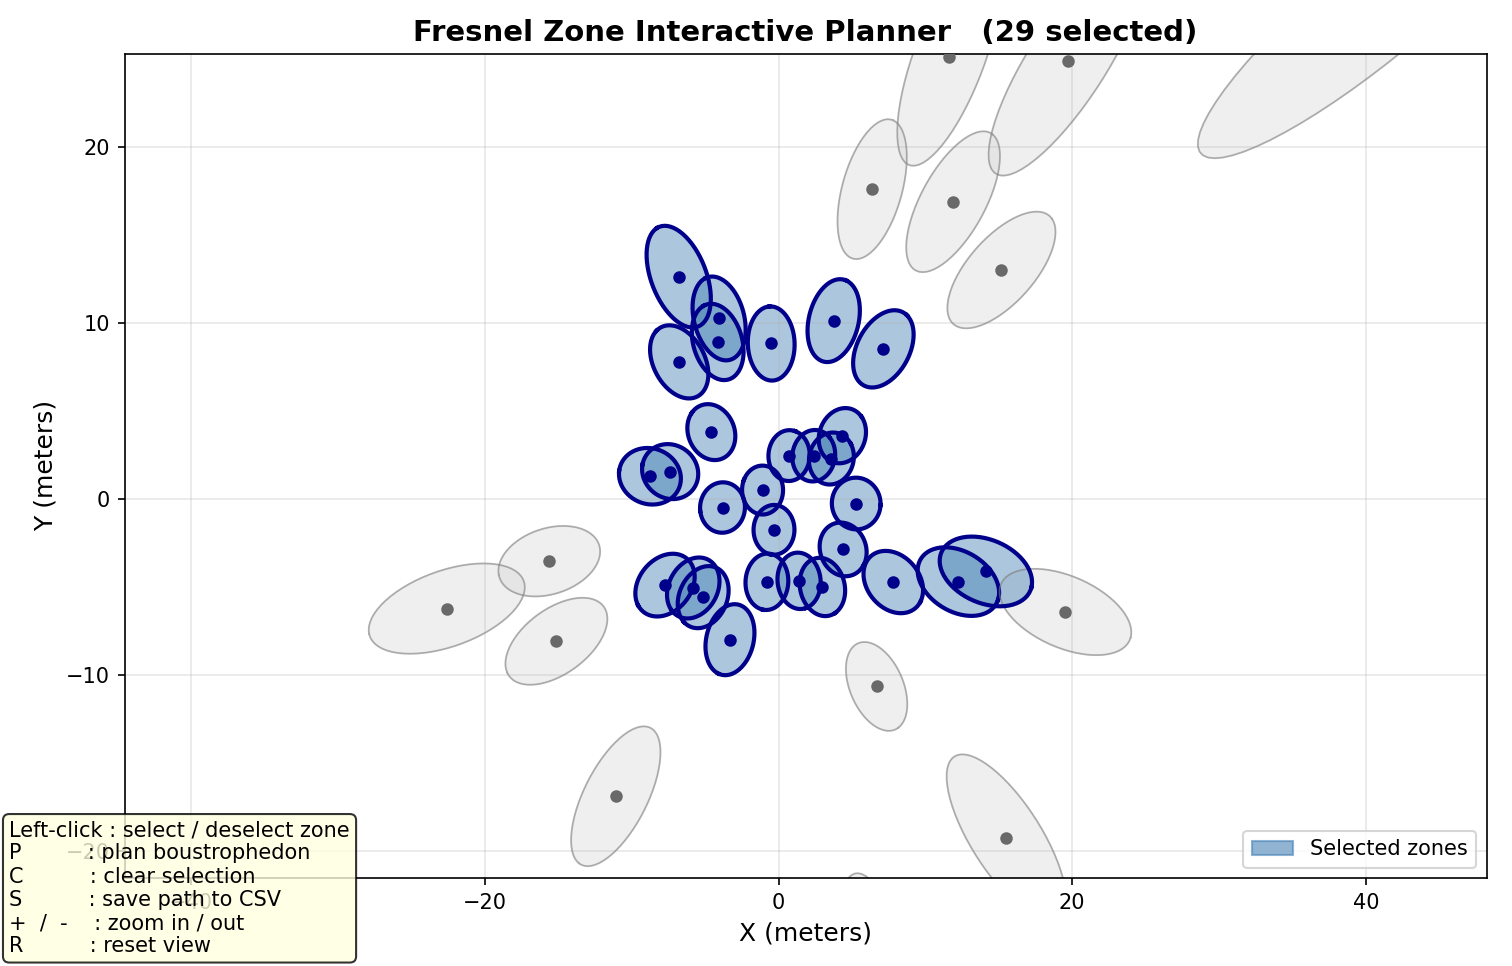
\includegraphics[width=0.8\textwidth]{Included_Images/cluster.png}
    \caption{Fresnel zone cluster}
    \label{fig:cluster}
\end{figure}

\begin{figure}[H]
    \centering
    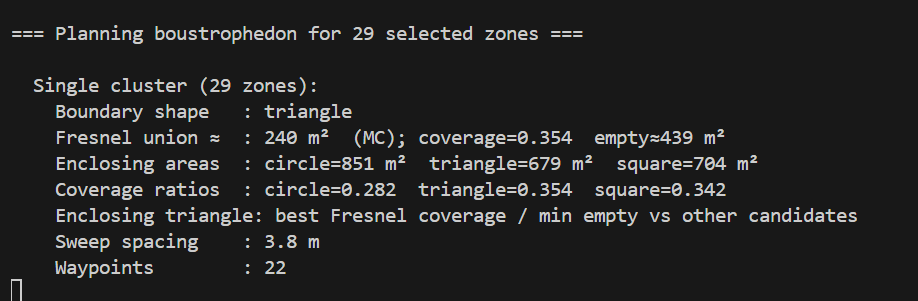
\includegraphics[width=0.8\textwidth]{Included_Images/area_calculation.png}
    \caption{Area calculation}
    \label{fig:detection_area}
\end{figure}

\begin{figure}[H]
    \centering
    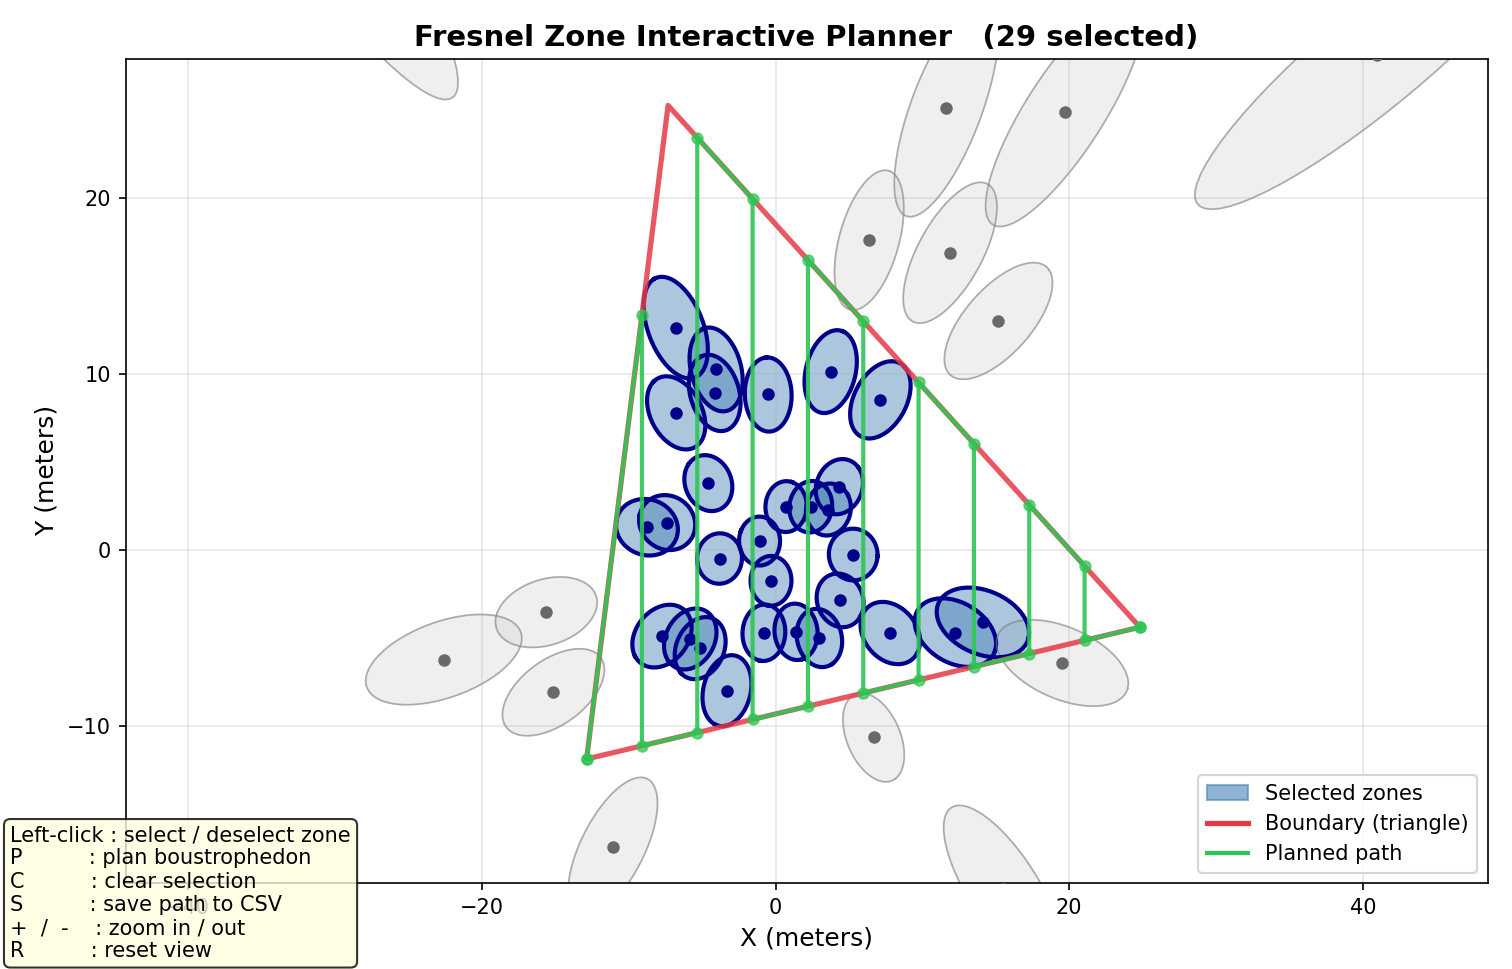
\includegraphics[width=0.9\textwidth]{Included_Images/boundary.png}
    \caption{Determined boundary}
    \label{fig:boundary}
\end{figure}

The process of obtaining the optimal detection area is illustrated from Figure \ref{fig:fresnel_zone_clustering} to
Figure \ref{fig:boundary}. In this example, the detection area is calculated for
all three shapes, and the optimal boundary is determined based on coverage
ratios. Among the three shapes, the triangle achieves the highest coverage ratio
of 0.354. Therefore, the algorithm selects the triangular boundary as the optimal
detection area.

\paragraph{Coverage Path Planning in QGroundControl} ~\\
The mission is defined by the parameters, such as the survey type, speed, space
and altitude, in QGroundControl. The space is the parameter that specifies the
sweeping distance. In addition, it is necessary to define the geo-fence and the
rally point (an alternative landing point) to ensure safety during the flight.
Then the mission can be uploaded to the Pixhawk flight controller via telemetry.
Figure \ref{fig:gqc_coverage} shows successful execution of the mission
conducted at Mount Davis Park in Hong Kong. 

\begin{figure}[H]
    \centering
    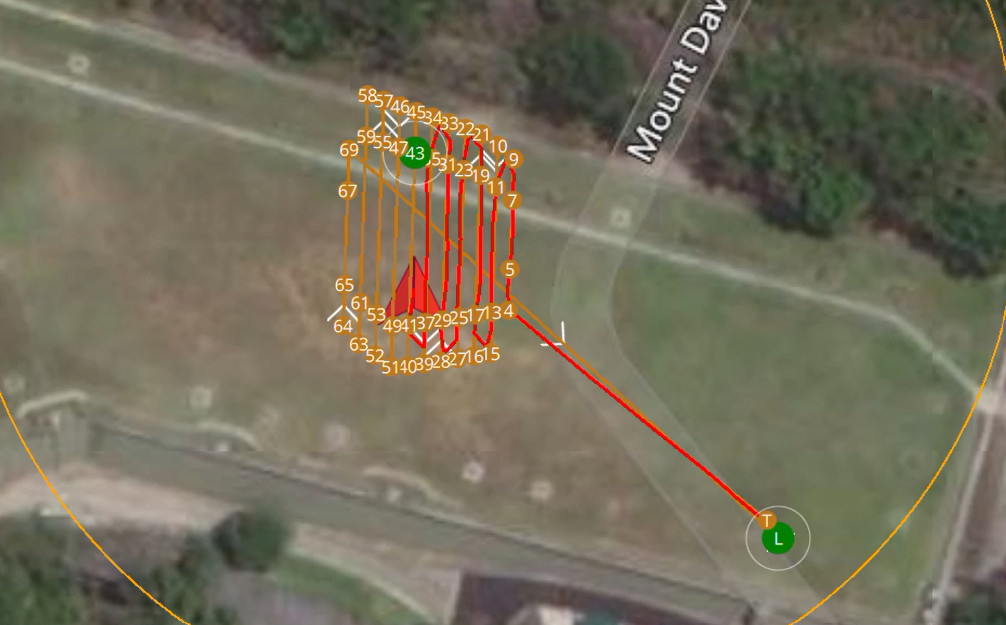
\includegraphics[width=0.8\textwidth]{Included_Images/gqc_coverage.png}
    \caption{Coverage path planning mission in QGroundControl}
    \label{fig:gqc_coverage}
\end{figure}

In summary, waypoint-based navigation experiments were conducted primarily to
hover the UAV above a tree or vegetation and above bare ground without trees.
This is mainly to assist in obtaining the differences in GNSS reflection over
vegetation and bare ground. Moreover, Fresnel zone clustering and coverage
path planning was implemented to achieve a reliable path planning workflow to
collect stronger GNSS reflected signals

In addition, coverage path planning was implemented to obtain dynamic UAV
movement data, which enables the development of LiDAR SLAM in our system. In our
system, LiDAR SLAM is developed to complement the GNSS-R analysis and Machine
Learning results. The section below discusses the LiDAR SLAM pipeline and the
results obtained from the real-world experiments.


% --- LiDAR SLAM ---
\section{LiDAR SLAM}

\subsection{Literature Review}
In recent years, autonomous robots have been widely implemented to carry out
repetitive tasks or take part in site surveys to ensure human safety or even
reduce operational cost. To carry out remote sensing via UAV, mapping is
essential for generating accurate three-dimensional representations of the environment. For tree canopy monitoring, 3D point cloud mapping provides additional spatial reference information by capturing canopy structure, height, and surface geometry, thereby complementing conventional remote sensing observations.

The common way to carry out mapping is by using sensors such as camera or LiDAR to create an odometry. This allows the robots to estimate their position and movement over time by measuring the changes in each
frame of the sensors. In practice, the common approaches to frame-to-frame
odometry are visual odometry or LiDAR odometry. Visual odometry estimates motion
by tracking distinct features in each image frame through gradients and textures
while LiDAR odometry uses laser range measurements to scan the environment.
Since our project focuses on investigating forests and dense vegetation, LiDAR
odometry is preferred as it is not affected by visually repetitive scenes and
varying lighting conditions that cause instability in camera-based methods. 

\subsubsection{LiDAR Odometry} 
The accuracy of LiDAR odometry largely depends on how well point clouds are
aligned, and it generally classified into point-based and feature-based
approaches. In terms of point-based point cloud registration, iterative closest
point (ICP) is considered one of the most well-known pointwise LiDAR odometry
methods. It is a simple, modular algorithm that aligns two consecutive point
clouds by establishing point-to-point correspondences and estimating the
transformation that minimizes their distance error \cite{besl1992method}.
However, a key limitation of ICP is its high cost for computation when registering
dense point clouds. Its accuracy relies strongly on the quality of the initial
alignment due to the non-convex nature of the optimization, and the presence of
outliers from moving objects can further complicate the process by adding extra
non-convexities \cite{maron2016point}. To counter the limitation of ICP, variants
such as Generalized ICP (G-ICP), FASTG-ICP, Voxelized G-ICP (VGICP) have been
developed to improve its computational efficiency \cite{segal2009generalized,
huang2022point}. 

On the other hand, feature-based LiDAR odometry methods utilize a set of
representative features of the point clouds to calculate the required
transformation \cite{rusu2009fast, salti2014shot}. Fast Point Feature Histograms
(FPFH) is a feature-based point cloud matching method that looks at the distinct
shape in point clouds (surface normals) and uses multidimensional histogram to
label the geometric properties of each point \cite{rusu2009fast}. As FPFH is
able to remain consistent even if the sensor is rotated or moved, it creates a
robust tool for finding matches between different scans and can be used as an
initial alignment of point clouds before handling it to other types of
processors \cite{wu2020iterative}. However, creating complex descriptors for
every point is computationally expensive which is not favorable for real time
requirements \cite{doi:10.3233/AIC-230217}. 

In the meantime, LOAM uses more efficient way to carry out feature-based LiDAR
odometry. It is done by extracting features and edges within the point clouds
based on the smoothness of the point cloud clusters \cite{huang2022point}.
Unlike conventional ICP methods that compare consecutive scans directly, LOAM
matches these extracted features against a continuously updated map of dense
edge features, creating a scan-to-map correspondence system. Since feature-based
methods process only a small fraction of the original point cloud data rather
than all raw points, they require substantially less computational power for
matching compared to G-ICP and NDT optimization processes. Feature-based methods
rely less on the accuracy of the initial pose estimate than point-wise methods,
but this reduced dependence often results in noticeable drift along the altitude
axis. \cite{koide2021voxelized, shan2018lego}. In this case, LOAM variants such
as Lightweight and ground optimized (LeGO)-LOAM \cite{shan2018lego} are proposed
to counter the drifting in altitude direction.

\subsubsection{Simultaneous Localization and Mapping (SLAM)}
While odometry provides the foundation for estimating local motion through
consecutive point cloud alignment, it lacks mechanisms such as loop closure and
mapping, making it prone to drift over time \cite{liu2019optimized,
thrun2000probabilistic}. Simultaneous Localization and Mapping (SLAM) extends
odometry by incorporating global optimization techniques, enabling both drift
correction and the construction of consistent long-term maps. Moreover, SLAM
frameworks naturally support sensor fusion, allowing data from multiple
modalities such as GNSS and LiDAR to be combined, which further enhances
localization robustness and mapping accuracy \cite{xu2022review, rs11091009}.

In terms of optimization strategies, SLAM methods can generally be divided into
two categories: filtering-based approaches and pose graph optimization
approaches. Filtering methods, such as the Extended Kalman Filter (EKF) or
particle filters, update the robot’s state incrementally as new sensor data
arrives, making them suitable for real-time applications but often less accurate
over long trajectories. In contrast, pose graph optimization such as GraphSLAM
treats past poses and sensor measurements as nodes and constraints in a graph,
allowing global corrections through nonlinear optimization. 

EKF SLAM is one of the fundamental SLAM algorithms within the filtering-based
approach. It estimates the system state through an iterative cycle of
prediction, observation, and correction, effectively functioning as a
specialized form of Bayesian filtering \cite{paz2007ekf}. Unlike pure
odometry-based methods, EKF SLAM incorporates implicit loop closure, where it
matches current observations to known landmarks. The filter then automatically
updates the estimated position and all correlated landmarks in the state vector
to reduce accumulated drift. While this mechanism improves consistency, it is
less flexible than the explicit loop closure in graph-based SLAM, which performs
global optimization \cite{khan2021comparative}. 

Although EKF SLAM is known to be used in real-time SLAM applications due to its
low-latency estimates, it faces quadratic complexity when updating the
covariance matrix with new landmarks, making it less scalable for large
environments but still efficient for small to medium-scale maps
\cite{gil2015occupancy}. Additionally, EKF SLAM integrates data from multiple
sensors by weighting each input according to its uncertainty, which helps manage
cross-sensor correlations \cite{oh2010symmetrical}. 

\begin{figure}[H]
    \centering
    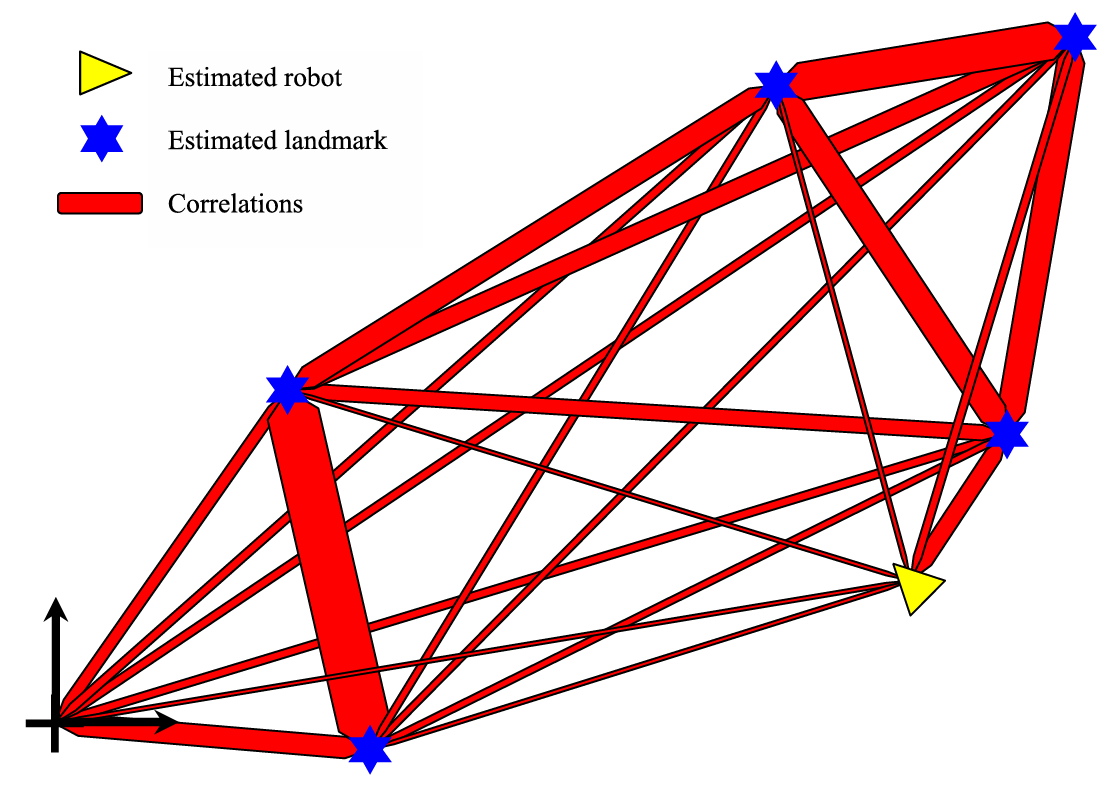
\includegraphics[width=0.7\textwidth]{Included_Images/EKF SLAM.png}
    \caption{The figure depicts a spring network analogy to visualize how EKF
SLAM works, with the red lines showing the correlations between landmarks. As
the robot passes a landmark more than once, these correlations increase, which
makes the red spring thicker \cite{stachniss2016simultaneous}.}
\end{figure}

GraphSLAM on the other hand is an algorithm designed for the offline SLAM
problem, where pose graph optimization is employed to refine the robot’s
trajectory by minimizing errors across a graph of poses and constraints. Similar
to EKF SLAM, GraphSLAM uses Bayes’ rule for probabilistic inference and similar
methods for building motion and measurement models \cite{thrun2006graph}. The key difference
between GraphSLAM and EKF SLAM is that GraphSLAM requires to accumulate all
data first before process everything together. This makes it more
computationally heavy as solving the resulting large optimization problem often
involves costly operations such as matrix inversion. To address this, GraphSLAM
applies iterative optimization methods like stochastic gradient descent \cite{bosse2004simultaneous},
which adaptively solve the non-linear optimization problem more efficiently,
while alternatives such as conjugate gradient methods can further improve
scalability. \cite{konolige2004large}

Moreover, GraphSLAM explicitly incorporates loop closure. Which means that when
the robot revisits a previously mapped location, it recognizes the place and
adds new constraints linking the current pose to the past one. This additional
relation corrects accumulated drift and improves global consistency
\cite{grisetti2011tutorial}. Based on \cite{konolige2004large,
montemerlo2006large}, GraphSLAM can refer to more than 100 million environments
features, as each robot pose only connects to adjacent poses and each feature
only connects to poses where it was observed without connecting to each other. 

\begin{figure}[H]
    \centering
    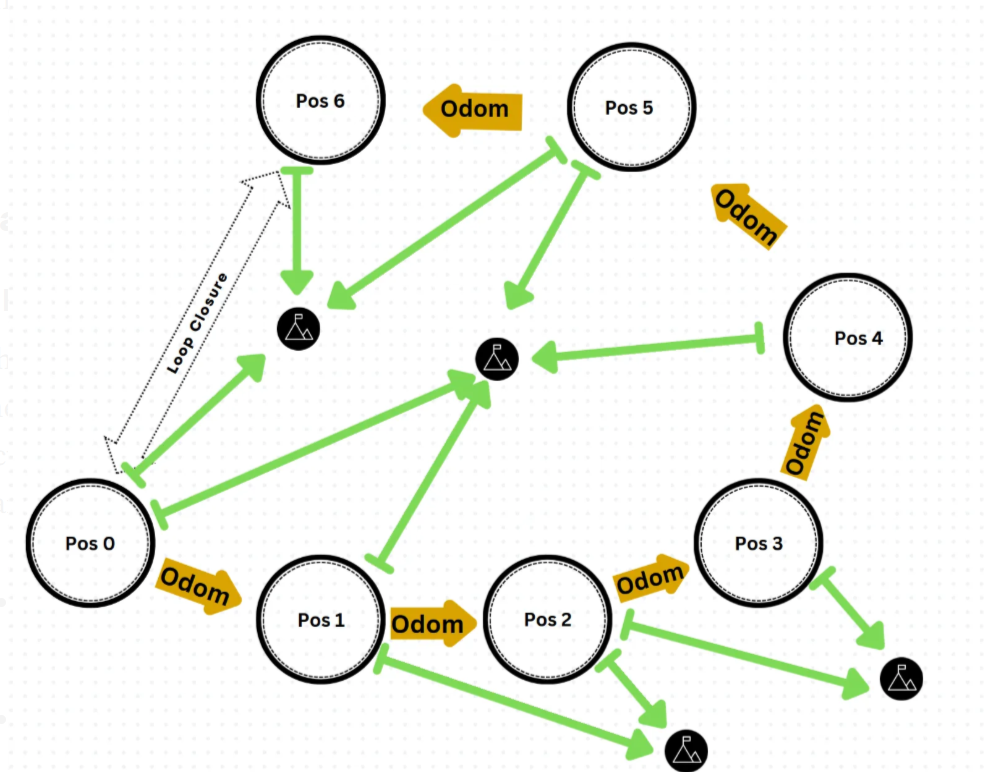
\includegraphics[width=0.7\textwidth]{Included_Images/pgo.png}
    \caption{Visualization of GraphSLAM with loop closure.}
\end{figure}

Although GraphSLAM is more robust than EKF-SLAM and both approaches have
demonstrated strong performance in urban and structured environments
\cite{mailka2024efficient, rs11091009} single-sensor SLAM systems (e.g.
LiDAR-only) remain vulnerable to drift because their measurements are purely
relative, allowing errors to accumulate over time. While recent work such as
\cite{mailka2024efficient}has integrated additional sensors to improve SLAM
accuracy, their applicability to UAV-based forest monitoring remains limited due
to canopy interference, sparse LiDAR features, and computational trade-offs.
As a result, this project investigates how the combination of filter-based odometry and graph-based SLAM with GPS constraints can be adapted and deployed for real-time forestry applications.

\subsection{Methodology}
This section describes the methodology adopted to develop the proposed GPS-aided modular SLAM system for UAV remote sensing with the aim to reduce trajectory drift. To achieve this, the methodology is divided into several key components. First, Fast-LIO is used as the front-end odometry to fuse LiDAR and IMU data using an Iterative Extended Kalman Filter (IEKF) for real-time pose estimation and local map generation. Second, back-end optimization SLAM is employed to carry out trajectory refinement and loop closure detection with GPS measurements to provide constraints. Third, frame transformation between GPS and LiDAR is carried out to align both data sources into the same coordinate system. Lastly, the complete system architecture is outlined to illustrate how the sensing, front-end estimation, and back-end optimization modules are interacted within the Robotic Operating System (ROS).

\subsubsection{LiDAR-Inertial Odometry}
For the front end of the modular SLAM system, LiDAR-Inertial Odometry (Fast-LIO)
is used to build a map effectively within a short amount of time. To do this,
Iterative Extended Kalman Filter (IEKF) is used to combine the data between IMU and LiDAR
point clouds to create an odometry of the environment. 

Iterative Extended Kalman Filter (IEKF) follows the core of Bayesian Recursion
to estimate the state of the robot through the prediction and measurement update
step. In the prediction step, IEKF presumes that the state of the system at time
$k$ is evolved from the previous system state at time $k-1$, and it is shown as
follows:
\begin{equation}
    x_k = f(x_{k-1},u_k) + w_{k} 
\end{equation}

Where $x_k$ is the state vector of the system's terms of interest at time $k$.
The $f(.)$ represents a non-linear state function that is used to forecast
current state data from prior state data $x_{k-1}$ and $u_k$ is a control
vector. We can approximate $w_{k-1}$ as $N(0,Q_k)$ where it is distributed
according to a multivariate normal distribution with zero mean and covariance
matrix $Q_k$.

To know the uncertainty of the prediction model, error covariance matrix $P^f_k$
is defined as shown:
\begin{align}
    P_k^f &= E\left(e_k^f(e_k^f)^T\right) \nonumber \\
    &\approx F_k E(e_{k-1}e_{k-1}^T)F_k^T + E(w_{k-1}w_{k-1}^T) \nonumber \\
    &= F_kP_{k-1}F_k^T + Q_{k-1}
\end{align}

Where $e$ is the prediction error, $F$ is the Jacobian matrix of the linearized
state transition function $f(.)$ evaluated at the previous estimate $x_{k-1}$,
and $Q$ is characterized as the noise covariance matrix associated with the
uncertainty of the physical model.

Even so, the predicted state alone is prone to errors due to various
factors such as inaccurate prediction function and further source of noise. This
issue can be solved by taking sensor measurements to improve the predicted state
accuracy. Hence, the observation model is defined as shown:
\begin{equation}
    z_k = h(x_k) + v_k
\end{equation} 

Where $z_k$ represents the expected sensor measurements based on the predicted
state $x_k$ expressed by a non-linear function $h(.)$, and the observation noise
$v_k$ is assumed as $N(0,R_k)$ where it has zero mean with covariance matrix $R_k$.

To further improve the accuracy for the nonlinear system, an iteration index
$K$ is added to repeat the measurement update at time step $k$ as shown:
\begin{equation}
    x^a_{k,K=0} = x^f_k
\end{equation}

Where $x^a$ is the state estimate after corrected by sensor measurement and
$x^f$ is the predictive distribution before looking at the LiDAR data. In this
case, the iteration $K$ is repeated until the change in the state estimate
$|x^a_{k,K+1} - x^a_{k,K}|$ falls below threshold $\epsilon$. 

As actual measurements from sensors will typically differ from this prediction
due to sensor noise and model inaccuracies, it is incorporated into the state
estimate by computing the difference between the actual measurements and the
predicted measurement at the present iterative estimate $K$:
\begin{equation}
    z_{k, K} = z_k - h(x^a_{k, K})
\end{equation}
Where $h(x^a_{k, K})$ is the non-linear observation function evaluated at the
most recent estimate. To balance the uncertainty of the prediction against the
new sensor data, the Kalman Gain $K_{k,K}$ is calculated using the state-space
dimension formula \cite{xu2021fast}.
\begin{equation} 
    K_{k, K} = (H_{k, K}^T R_k^{-1} H_{k, K} + (P_k^f)^{-1})^{-1} H_{k, K}^T R_k^{-1} 
\end{equation}

Where $H_{k, K}$ is the Jacobian of the observation function re-evaluated
at the present iterative estimate $x^a_{k, K}$. This gain is then used
to compute the next refined state estimate:
\begin{equation}
    x^a_{k,K+1} = x^a_{k, K} + K_{k, K} (z_{k, K}) - (I - K_{k, K} H_{k, K})(x^a_{k, K} - x_k^f)
\end{equation}

After updating the state estimate, the updated covariance of the state
distribution is given as:
\begin{equation} 
    P_k = (I - K_{k, K} H_{k, K}) P_k^f 
\end{equation}

While the IEKF provides a high-frequency estimate of the current state, the
overall SLAM problem can be generalized as a Maximum A Posteriori (MAP)
estimation. Bayes Filter is then used to recursively perform the state
prediction and measurement update steps to minimizes linearization errors for
robust localization. In this case, MAP can be expressed as:
\begin{equation}
    P(X|Z, U) \propto P(x_0) \prod_{k} P(z_k|x_k) \prod_{k} P(x_k|x_{k-1}, u_{k-1})
\end{equation}

Where $P(X|Z, U)$ is the refined state estimate, $P(x_0)$ is the prior,
$P(z_k|x_k)$ is the sensor measurement and $P(x_k|x_{k-1}, u_{k-1})$ is the
predicted state.

\begin{figure}[H]
    \centering
    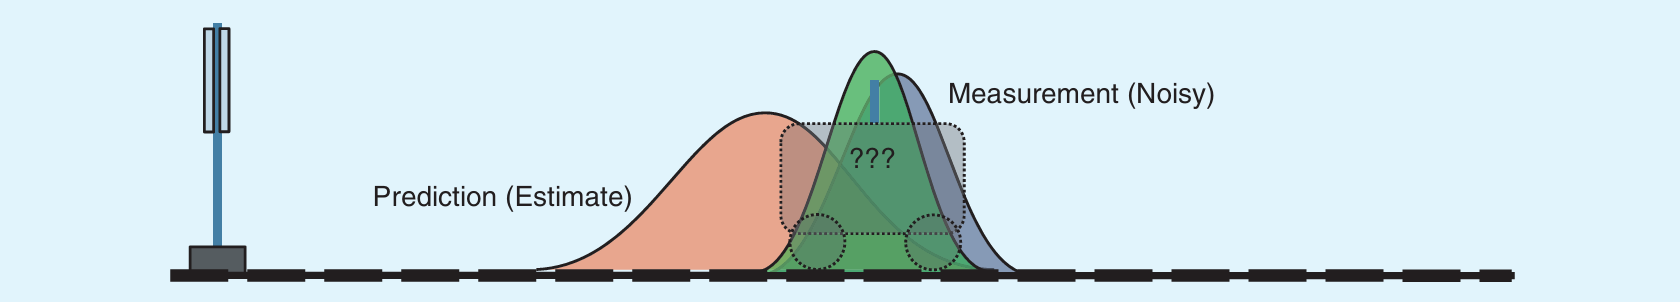
\includegraphics[width=\textwidth]{Included_Images/Kalman Filter.png}
    \caption{The red distribution in the figure represents the predicted step
    $P(x_k|x_{k-1}, u_{k-1})$ which results in predictive distribution $x^f_k$.
    The blue distribution represents likelihood $P(z_k|x_k)$ derived from the
    noisy sensor measurement $z_k$. The green distribution illustrates the
    refined state estimate $x^a_k$, showing the reduction in the uncertainty
    covariance $P_k$ after fusing both data sources
    \cite{faragher2012understanding}.}
\end{figure}

\subsubsection{Graph-Based SLAM with GPS}
As LiDAR odometry is employed in the front end to provide high-rate local pose estimates, it mainly relies on relative motion information and does not include global constraints. Consequently, small scan-matching and motion estimation errors may accumulate over time, leading to trajectory drift and map distortion. This limitation can persist even in LiDAR-based SLAM systems with robust mapping and loop closure, particularly in large-scale environments where relative errors continue to propagate \cite{cwian2021large, chen2022slam}. To address this issue, a back-end optimization framework is employed via implementing graph-based SLAM with loosely coupled GPS measurements. In this case, the graph-based optimizer helps to refine all robot poses over the full trajectory, while GPS data provides absolute positional constraints to anchor the trajectory and improve global consistency.

In graph-based SLAM, bipartite probabilistic graphical model is used to represent the estimation problem in a structured way. Each node of the graph corresponds to the robot pose at a particular time step, typically containing the robot’s position and orientation. In addition, each factor represents a constraint or relationship between one or more pose nodes. This can be derived from available information such as the motion model, LiDAR scan matching, loop closure observations, or GPS measurements. Based on that, the estimation problem can also be expressed using Maximum A Posteriori (MAP) inference to factorize the collective posterior distribution of the trajectory state $X$ as shown \cite{wen2021factor}:

\begin{equation} 
    P(X|Z, U) \propto P(x_0) \prod_{k} P(z_k|x_k) \prod_{k} P(x_k|x_{k-1}, u_{k-1}) 
\end{equation}

where $P(x_0)$ is the prior distribution of the initial pose, $P(z_k|x_k)$ represents observation factors such as GPS measurements, and $P(x_k|x_{k-1}, u_{k-1})$ represents odometry factors derived from the relative pose estimates of the front-end LiDAR odometry. 

Assuming Gaussian noise, the odometry and observation factors can be expressed in exponential form. Unlike the standard filtering calculations that only estimates the current state $x_k$, the factorized graph maintains the entire trajectory history $X$ = ($x_0, x_1, \dots, x_k$) to minimize the sum of squared errors. With that, the odometry factor between two consecutive poses is written as
\begin{equation}
    P(x_k|x_{k-1},u_{k-1}) = \exp(-||f_k(x_{k-1}, u_k)-x_k||^2_{\Sigma_{u,k}})
\end{equation}

where $f_k(x_{k-1}, u_k)$ indicates the relative motion estimate from the front-end LiDAR odometry and $\Sigma_{u,k}$ is its covariance. Similarly for the observation factor, which correspond to the GPS measurements can be written as:
\begin{equation}
    P(z_k^{gps}|x_k) = \exp\left(-\|p_k - z_k^{gps}\|^2_{\Sigma_{gps,k}}\right)
\end{equation}

where $p_k$ is the estimated robot's position in the SLAM calculation, $z_k^{gps}$ is the GPS position measurement at time step $k$, and $\Sigma_{gps,k}$ is the covariance associated with the GPS measurement. 

By taking the negative logarithm of the posterior distribution, the MAP problem is converted into a nonlinear least-squares optimization problem:
\begin{equation} \label{arg_min}
    \hat{\chi} = \arg\max_{\chi} \prod_{k} F_k(x_k) = \arg\min_{\chi} F(\chi)
\end{equation}

Based on Equation \eqref{arg_min}, it evaluates how well the estimated trajectory satisfies both the relative LiDAR odometry constraints and the absolute GPS constraints. In the specific case of LiDAR odometry and GPS fusion, the cost function represents the total error in the estimated trajectory where the optimization aims to find the state $X$ that minimizes this error. Thus, the equation can be written as shown:
\begin{equation} \label{eq:error_score}
F(X)=\sum_i \left\| e_{i,i+1} \right\|^2_{\Omega_{odom}}
\;+\;
\sum_k \left\| z_k^{gps} - p_k \right\|^2_{\Omega_{gps}}
\end{equation}

where $e_{i,i+1}$ denotes the residual associated with LiDAR odometry factor between two consecutive poses. This indicates the mismatch between the relative motion estimated by the front-end LiDAR odometry and the relative displacement implied by the optimized poses. Meanwhile, $\Omega_{odom}$ is the information matrix representing the uncertainty of LiDAR odometry and $\Omega_{gps}$ is the information matrix of GPS uncertainty. These matrices are then used to determine how much influence each measurement source has in the optimization process. Measurements with lower uncertainty are given higher influence during optimization, while noisier measurements contribute less to the final solution. 

Since the total cost function $F(X)$ is generally nonlinear with respect to the robot states, iterative nonlinear least-squares methods are used to solve this problem by using Levenberg-Marquardt algorithm. It is a standard optimization method used to iteratively solve for the trajectory update using the Jacobian matrix \cite{ranganathan2004levenberg}. In each iteration, the nonlinear error function is linearized around the current state estimate and an increment $\Delta X$ is computed to update the pose estimate until convergence is achieved. The state update $\Delta X$ can be expressed as:
\begin{equation}
\Delta X = -(J^T \Omega J + \lambda \text{diag}(J^T \Omega J))^{-1} J^T \Omega e
\end{equation}

where the residual $e$ denotes the error between the LiDAR odometry and GPS measurement, the Jacobian $J$ denotes the first-order partial derivatives of the residuals $e$ with respect to state variable $X$, the information matrix $\Omega$ represents the global stacked information matrix containing all measurement weights, and the damping factor $\lambda$ is used to regulate the update step by balancing the behavior between the Gauss-Newton method and gradient descent. Once the state update $\Delta X$ is calculated, it can be used to calculate the new state estimate, resulting in higher SLAM accuracy.
\begin{equation}
    \mathcal{X}^{(i+1)} = \mathcal{X}^{(i)} + \Delta \mathcal{X}
\end{equation}

Even though Levenberg-Marquardt algorithm is able to solve the whole robot's trajectory at once, the matrices can get too large to invert in real-time if the robot continues to drive. Therefore, the actual implementation uses iSAM2 which converts the mathematical problem into Bayes Tree to perform incremental updates in real time more efficiently \cite{kaess2012isam2}. With that, only the affected portions of the factor graph are updated when new LiDAR odometry, GPS observations, or loop closure constraints are introduced. This in turn reduces the computational complexity of the SLAM system while preserving its estimation accuracy for real-time operation.

The iterative optimization process described above is summarized in Figure \ref{fig:pgo_framework}. Starting from the current trajectory estimate, the total residual error is evaluated, and the nonlinear system is linearized around the operating point. A correction term is then solved and used to update the state estimate. This procedure is repeated until convergence is achieved to form a progressively refined trajectory.
\begin{figure}[H]
    \centering
    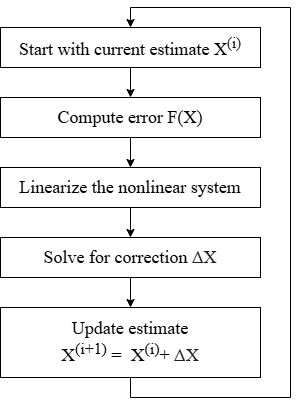
\includegraphics[width=0.4\textwidth]{Included_Images/gps_correction.png}
    \caption{Flowchart showcasing the iterative optimization loop for updating the robot state estimate.}
    \label{fig:pgo_framework}
\end{figure}

As a result, the proposed loosely coupled LiDAR-GPS graph-based SLAM framework combines the short-term local accuracy of LiDAR odometry with the long-term global stability of GPS measurements. This enables the robot to generate a globally consistent map while maintaining robust localization performance in large-scale outdoor environments.


\subsubsection{Frame Transformation}
With the aim of performing GPS correction in a pose graph SLAM system, LiDAR and GPS must be in the same coordinate frame in order to enable consistent comparison and fusion of their measurements during optimization. However, since the LiDAR sensor and GPS antenna are mounted at different physical location on the UAV, the relative transformation between the LiDAR and GPS coordinate frames must first be determined so that their measurements can be transformed into a common reference frame before GPS constraints are incorporated into the pose graph optimization process.
\begin{figure}[H]
    \centering
    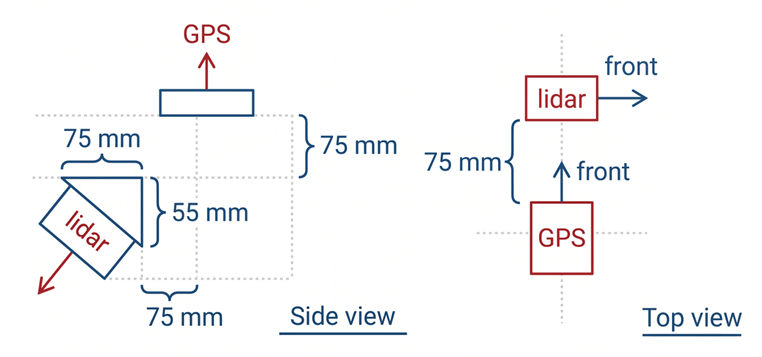
\includegraphics[width=0.75\textwidth]{Included_Images/lidar_pos.png}
    \caption{Illustration of the sensors' location on UAV.}
\end{figure}

Frame transformation consist of rotational and translational components that describe the relative orientation and positional offset between two coordinate frames. As the translational difference between LiDAR and GPS are at centimeter level which is insignificant within the SLAM system, only rotational transformation will be focused on in this case. 

To effectively perform frame transformation between two sensors, it is first necessary to determine how the coordinate frame axes are defined within the system. This was achieved by applying rotational offsets independently about each principal axis then observe the resulting change in sensor orientation. By isolating each rotational component, the direction and convention of rotation for each axis could be identified as shown in Figure \ref{fig:SLAM_axis}.
\begin{figure}[H]
    \centering
    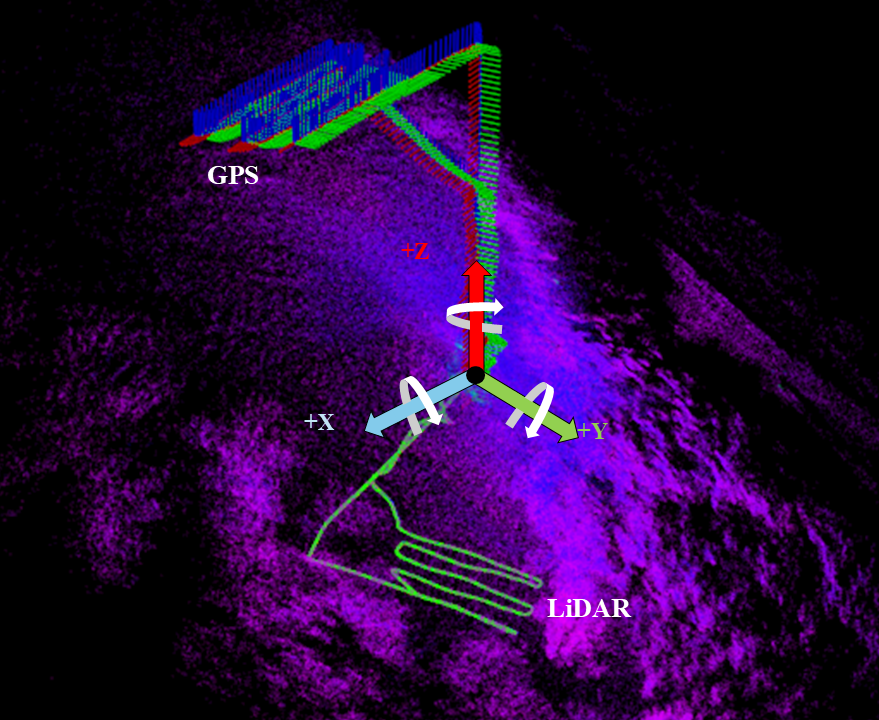
\includegraphics[width=0.7\textwidth]{Included_Images/SLAM_axis.png}
    \caption{Illustration of the direction of principal axis within SLAM system.}
    \label{fig:SLAM_axis}
\end{figure}

Meanwhile, as GPS only provide translational data such as longitude, latitude, and altitude, additional IMU which is located at the same position as the GPS antenna, is used to provide the rotational information for GPS measurement, creating a complete 6-DoF pose representation required for accurate frame transformation. Based on that, extrinsic calibration is carried out between the GPS/IMU and LiDAR/IMU systems to obtain the relative rotation between two sensor frames \cite{lidar_imu_init}. The calibration results indicate that there is a rotational offset of $145.98^\circ$ in roll, $90.0^\circ$ in yaw, and no rotational offset in pitch between the GPS and LiDAR frames. 

In an effort to implement the calibration results into the SLAM framework, the absolute initial heading of the LiDAR must be determined at the start of the system. This is because the LiDAR odometry defines its origin as $0^\circ$ based on the initial orientation of the UAV. Conversely, the GPS/IMU system operates in a global reference frame which is aware of the heading of East, West, North, and South, resulting in the initial orientation of GPS/IMU generally being nonzero. This creates an unknown rotational offset between the LiDAR local frame and the global navigation frame.
\begin{figure}[H]
    \centering
    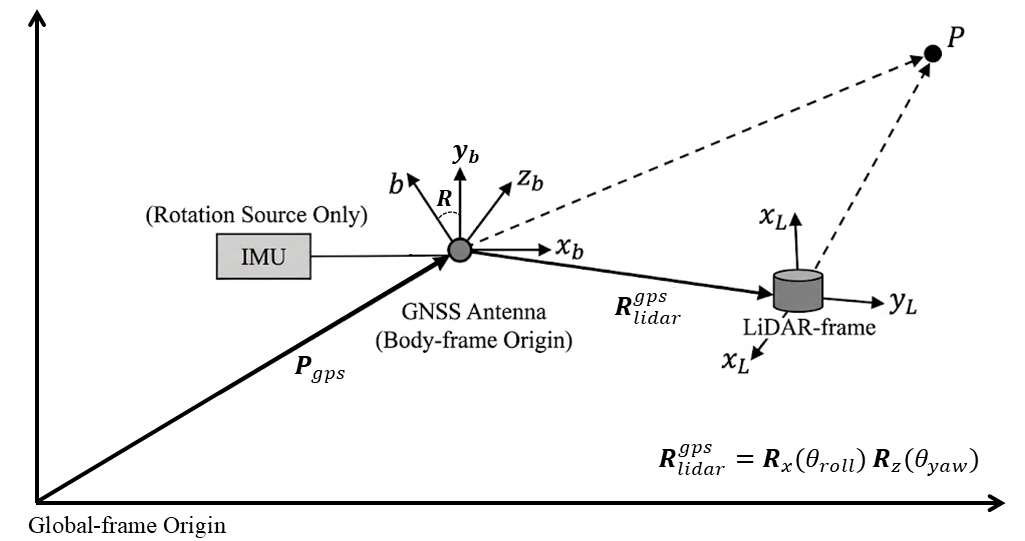
\includegraphics[width=0.8\textwidth]{Included_Images/frame_trans.png}
    \caption{Illustration of the frame reference frame of GPS and LiDAR.}
\end{figure}

To bridge this gap, initial IMU's global orientation from the GPS is captured at system startup and its represented as quaternion $Q_{imu\_global}$. Even so, given that GPS/IMU is rigidly attached to the LiDAR sensor via a known extrinsic calibration, its orientation must be corrected by the previously determined fixed transformation between the IMU and LiDAR frames where the transformation is represented as $Q_{imu\_to\_lidar}$. Thus, the absolute orientation of LiDAR with respect to global coordinate frame $Q_{lidar\_global}$ is therefore computed via quaternion multiplication chain:
\begin{equation}
Q_{lidar\_global} = Q_{imu\_global} \otimes Q_{imu\_to\_lidar}
\end{equation}

Once the absolute global orientation of the LiDAR is calculated, the system isolates the yaw heading component. Isolating the yaw is critical because pitch and roll are typically constrained by the IMU's gravity vector, meaning both the LiDAR/IMU and GPS/IMU systems have near-zero pitch and roll during initialization. This leaves the yaw heading as the primary unaligned degree of freedom between the local LiDAR frame and the global navigation frame.

The extracted initial yaw offset is stored and combined with the calibrated roll offset to construct the transformation matrix between GPS and LiDAR frames. The complete rotational compensation is expressed as:
\begin{equation}
P_{lidar} = R_x(\theta_{roll})\,R_z(\theta_{yaw})\,P_{gps}
\end{equation}
where $R_x(\theta_{roll})$ is the fixed roll rotation of $145.98^\circ$ and $R_z(\theta_{yaw})$ is the initial yaw alignment between the global GPS frame and the local LiDAR frame. This transformation matrix is then applied to every GPS measurement before it is being added into the pose graph. As a result, all GPS positions are converted into the LiDAR local coordinate frame, allowing GPS factors to be consistently fused with LiDAR odometry during pose graph optimization.

\begin{figure}[H]
    \centering
    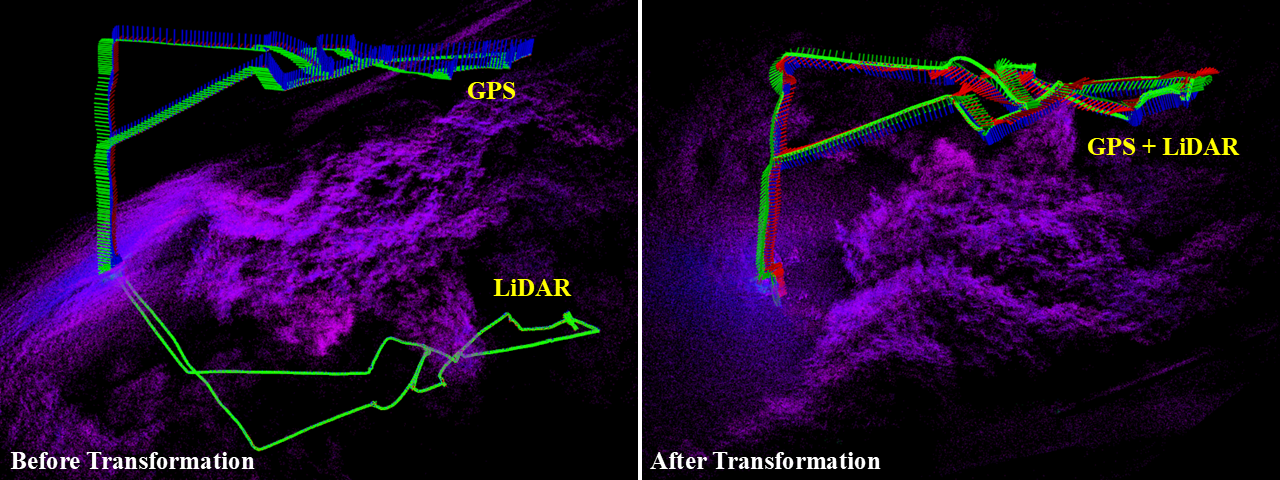
\includegraphics[width=1.0\textwidth]{Included_Images/transformation_result.png}
    \caption{Comparison of SLAM system before and after frame transformation.}
\end{figure}


\subsubsection{System Architecture}
In this project, a modular SLAM system is used with the front end having a
Fast-LIO LiDAR odometry to carry out mapping in real time, while Pose Graph
Optimization (PGO) coupled with GPS is used for the back end. During
implementation, both Fast-LIO and PGO are initialized. The point cloud data will
first be processed by Fast-LIO to create an odometry, and the odometry will then
be passed to the PGO to further optimize the point clouds to increase accuracy.
In the meantime, GPS data is passed into PGO to provide constraints to the SLAM system.
\begin{figure}[H]
    \centering
    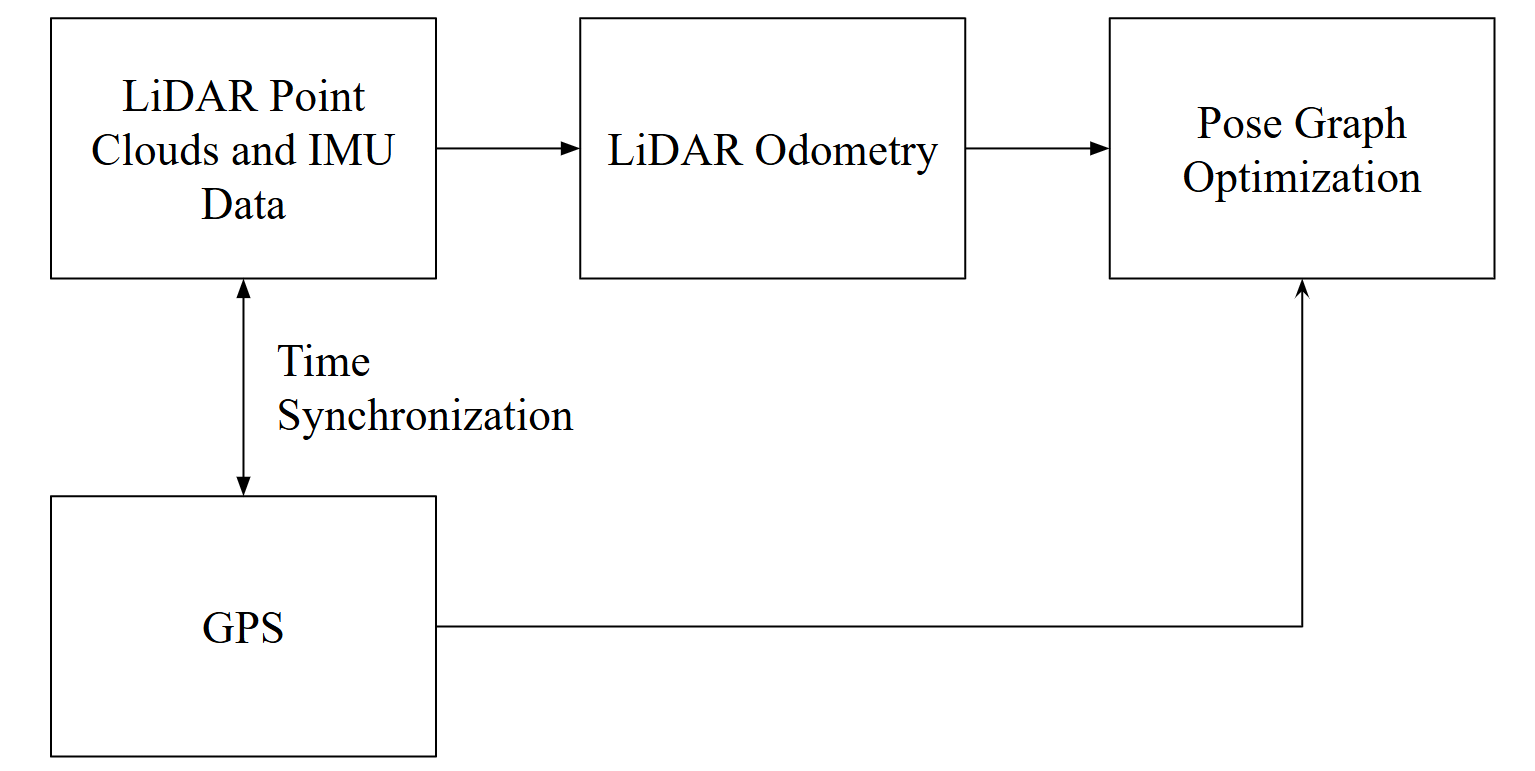
\includegraphics[width=0.75\textwidth]{Included_Images/SLAM flowchart.png}
    \caption{Flowchart of the modular SLAM system.}
\end{figure}


Based on Figure \ref{fig:rqt}, the system can be divided into sensor drivers, the front-end
LiDAR odometry, and back-end pose graph optimization (PGO) component. At the
sensor level, two main drivers are used. The Livox driver publishes raw LiDAR
and IMU data under the /livox namespace. In addition, the MAVROS driver
interfaces with the Pixhawk flight controller and publishes Pixhawk and GPS data
under the /mavros namespace.

The sensor data is then passed to the front-end LiDAR odometry (Fast-LIO) in the
/laserMapping node. It produces several outputs including: 
\begin{itemize}
    \item \texttt{/Odometry}: Real-time LiDAR odometry.
    \item \texttt{/path}: The estimated trajectory.
    \item \texttt{/cloud\_registered}: Point clouds aligned in the global frame.
    \item \texttt{/cloud\_registered\_body}: Point clouds in the body frame.
\end{itemize}

Afterward, topics including /Odometry and /path from Fast-LIO LiDAR Odometry,
/cloud\_ registered\_body from /laserMapping, and GPS and IMU information from
Pixhawk are passed to the back end pose graph optimization SLAM under
/laserPGO\_gps namespace. The optimized results are published as:
\begin{itemize}
    \item \texttt{/aft\_pgo\_odom}: Optimized odometry.
    \item \texttt{/GpsOdom}: GPS-constrained odometry.
    \item \texttt{/aft\_pgo\_path}: Globally optimized trajectory.
    \item \texttt{/aft\_pgo\_map}: Optimized global map.
    \item \texttt{/loop\_scan\_local} and \texttt{/loop\_submap\_local}: Data used for loop closure and local map refinement.
\end{itemize}
\begin{figure}[H]
    \centering
    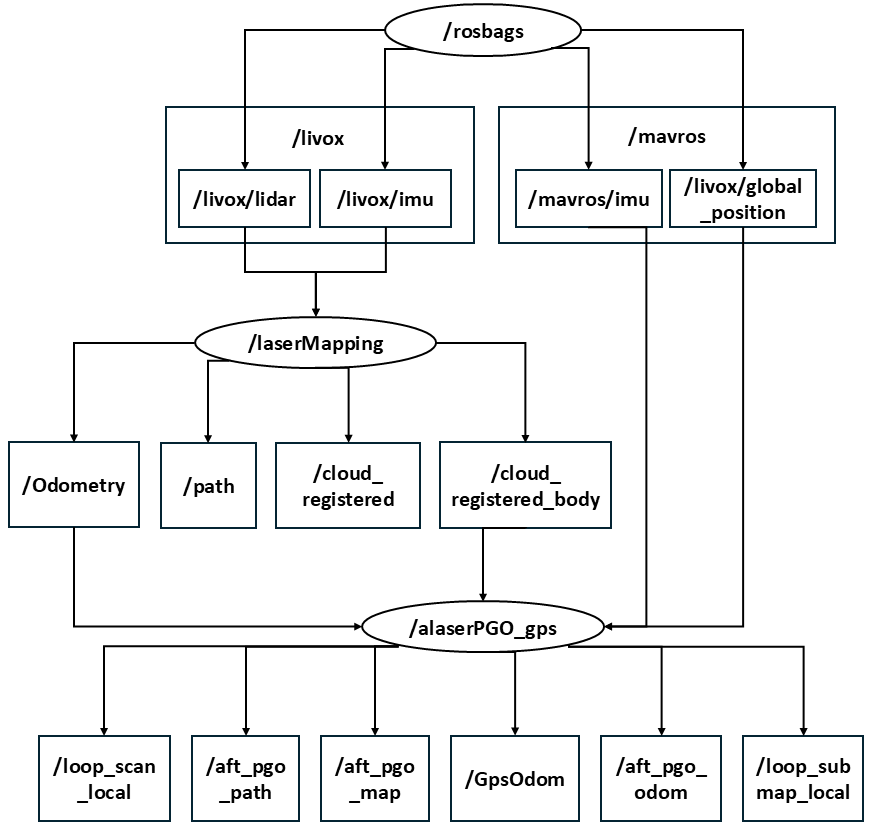
\includegraphics[width=0.9\textwidth]{Included_Images/rqt_graph.png}
    \caption{Interactions of different ROS topics in the SLAM system.}
    \label{fig:rqt}
\end{figure}

\subsection{Results and Discussion}
\subsubsection{Point Clouds Comparison}
To test the point cloud alignments, the same experiment data is run on Fast-LIO LiDAR Odometry, Pose Graph Optimization (PGO) SLAM without GPS, and PGO SLAM with GPS for comparison. 
\begin{figure}[H]
    \centering
    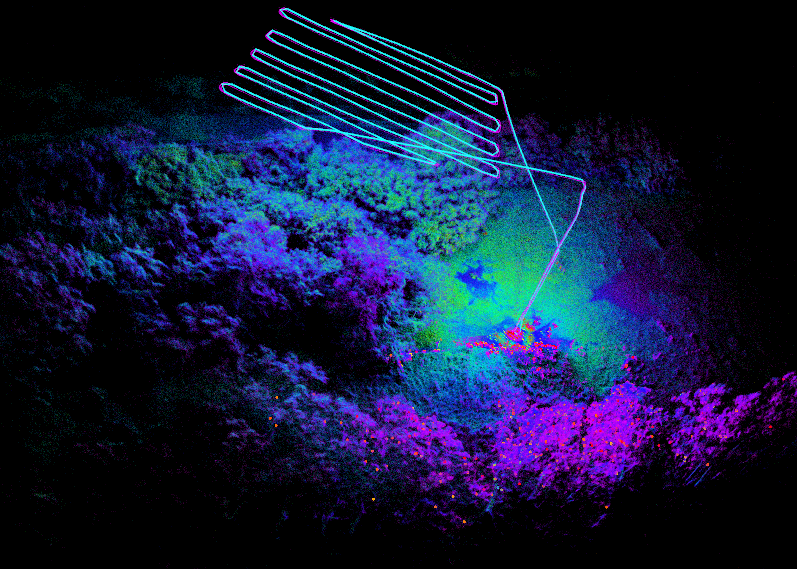
\includegraphics[width=0.75\textwidth]{Included_Images/rosbag3_FL.png}
    \caption{Fast-LIO LiDAR Odometry.}
    \label{fig:rosbag3_FL}
\end{figure}
\vspace{-3pt}
\begin{figure}[H]
    \centering
    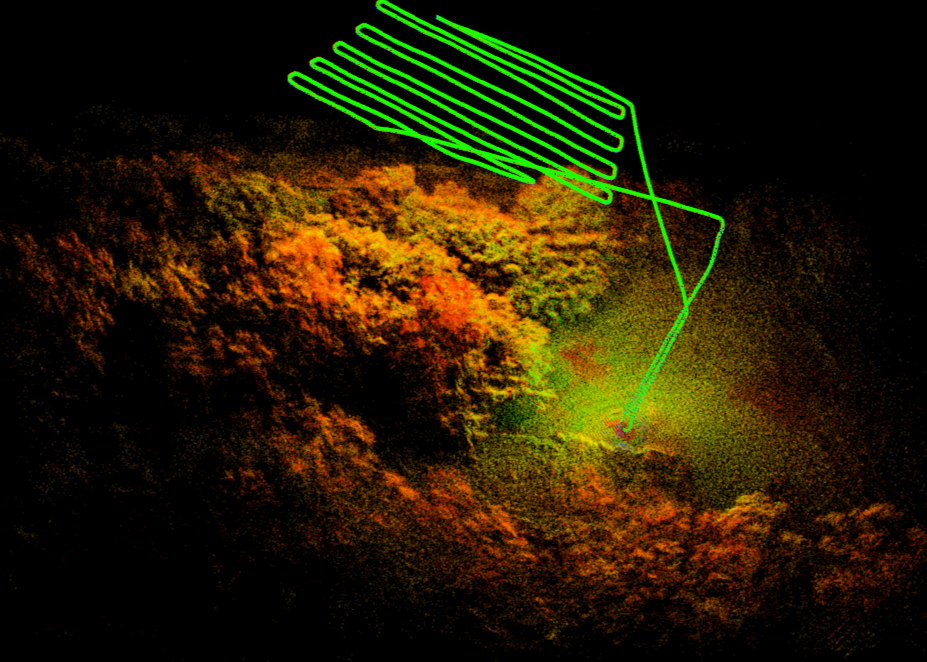
\includegraphics[width=0.75\textwidth]{Included_Images/rosbag3_pgo_nogps2.png}
    \caption{Pose Graph Optimization SLAM without GPS.}
    \label{fig:rosbag3_pgo_nogps}
\end{figure}
\vspace{-3pt}
\begin{figure}[H]
    \centering
    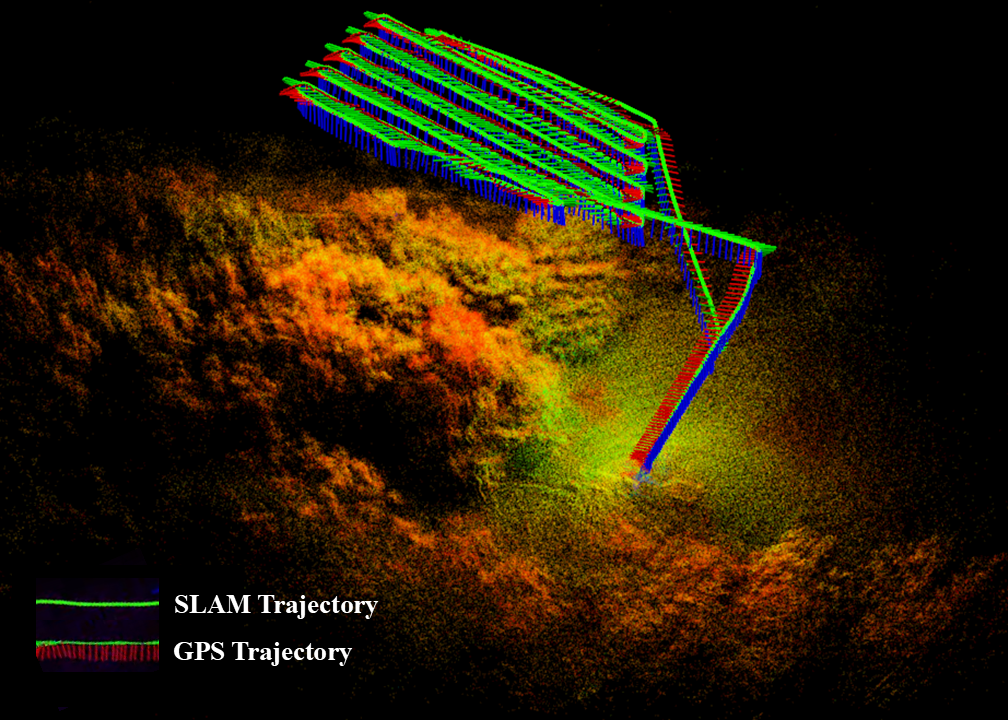
\includegraphics[width=0.75\textwidth]{Included_Images/rosbag3_pgo.png}
    \caption{Pose Graph Optimization SLAM with GPS.}
    \label{fig:rosbag3_pgo}
\end{figure}

When comparing Figure \ref{fig:rosbag3_FL}, Figure \ref{fig:rosbag3_pgo_nogps}, and Figure \ref{fig:rosbag3_pgo} that represents three approaches evaluated mentioned above, it is observed that the point cloud alignments are similar to each other. This shows that LiDAR odometry alone is already capable of producing a reasonably consistent local map and the integration of pose graph optimization and GPS constraints does not alter the structural alignment of the point clouds significantly. Even though there is not much difference in terms of the point cloud improvements with the additional pose graph SLAM system, the inclusion of GPS helps to improve global consistency by reducing long-term drift especially over larger trajectories or extended operation periods.

If the GPS trajectory and SLAM trajectory are not aligned, SLAM will consider GPS data to correct the SLAM poses, resulting the SLAM trajectory to align with the GPS trajectory. This can be investigated in the same dataset where we compare the PGO SLAM method that does not include GPS and the PGO SLAM method with GPS included. As illustrated in Figure \ref{fig:not_align} and Figure \ref{fig:align}, the trajectory obtained from PGO SLAM without GPS shows a noticeable misalignment between the estimated SLAM trajectory and the GPS reference trajectory. In contrast, optimized SLAM trajectory is more aligned with GPS trajectory when GPS constraints are incorporated into the SLAM calculation. Even so, GPS data is not always trustworthy. Incorporating all GPS measurements directly into the SLAM framework may degrade performance if low-quality data are included. As a result, filtering the high quality GPS data is essential for the accuracy of SLAM calculation. 

\begin{figure}[H]
    \centering
    \begin{subfigure}{0.4\textwidth}
        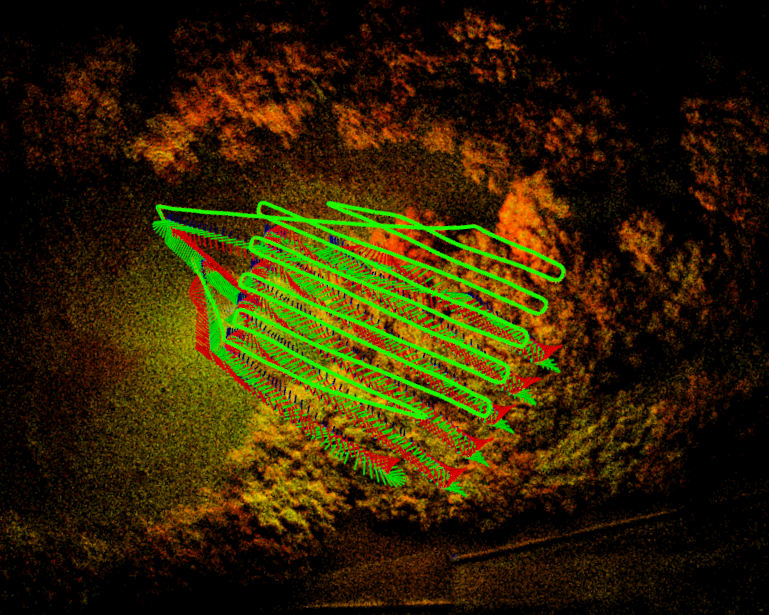
\includegraphics[width=\textwidth]{Included_Images/rosbag3_drift.png}
        \caption{Before including GPS data}
        \label{fig:not_align}
    \end{subfigure}
    \hfill
    \begin{subfigure}{0.4\textwidth}
        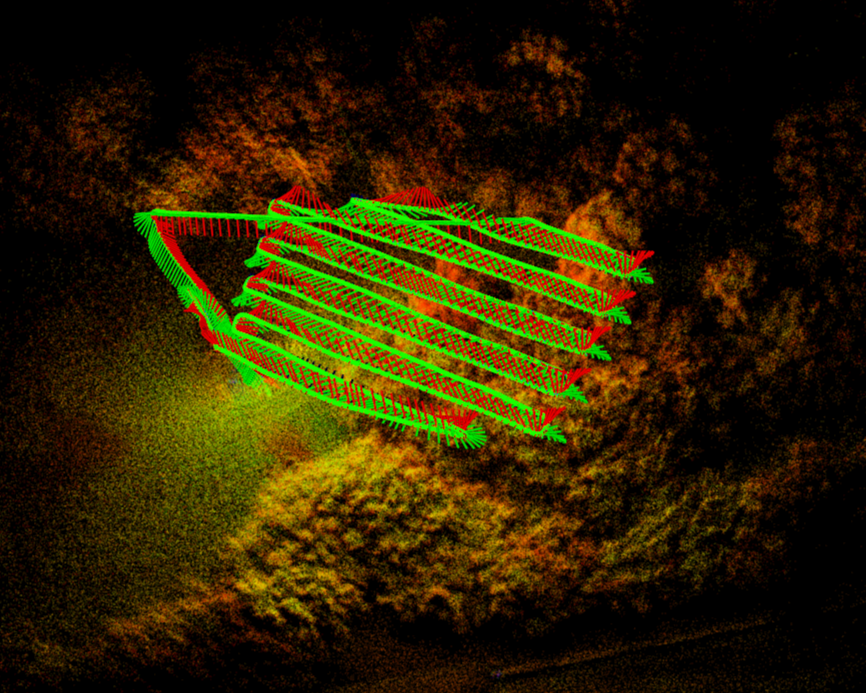
\includegraphics[width=\textwidth]{Included_Images/rosbag3_align.png}
        \caption{After including GPS data}
        \label{fig:align}
    \end{subfigure}
    \caption{Comparison of GPS inclusion in the pose graph SLAM system.}
\end{figure}

\subsubsection{GPS Data Filtering}
In order to only incorporate accurate GPS data for the SLAM calculation, a manually tuned covariance threshold is applied to filter out low-quality GPS data before they are added to the pose graph calculation. Thus, multiple covariance values are evaluated from a singular dataset (Data 2) to determine the appropriate threshold for the SLAM system. A lower threshold enforces stricter filtering, where it only retains high-confidence measurements. On the other hand, a higher threshold allows more GPS data to be incorporated with the risk of introducing noise.

\begin{figure}[H]
    \centering
    \begin{subfigure}{0.45\textwidth}
        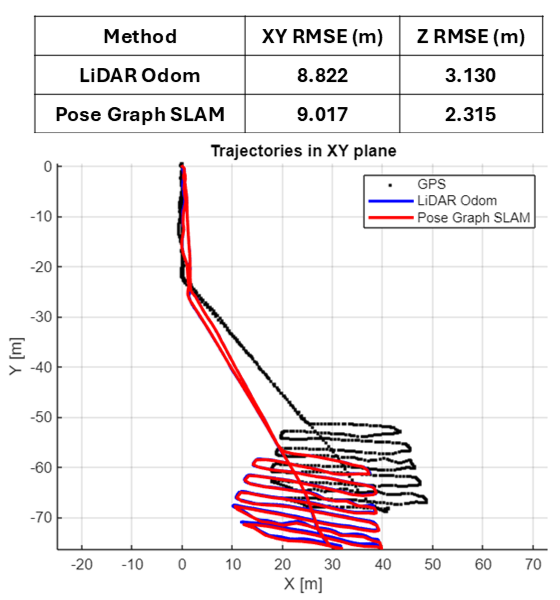
\includegraphics[width=\textwidth]{Included_Images/cov_0.01.png}
        \caption{Covariance Threshold = 0.01}
    \end{subfigure}
    \hfill
    \begin{subfigure}{0.45\textwidth}
        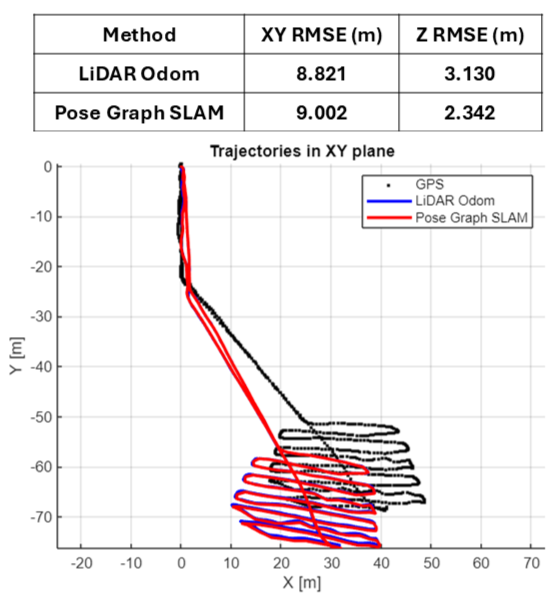
\includegraphics[width=\textwidth]{Included_Images/cov_0.03.png}
        \caption{Covariance Threshold = 0.03}
    \end{subfigure}
    \phantomcaption
\end{figure}
\begin{figure}[H]
    \ContinuedFloat
    \centering
    \begin{subfigure}{0.45\textwidth}
        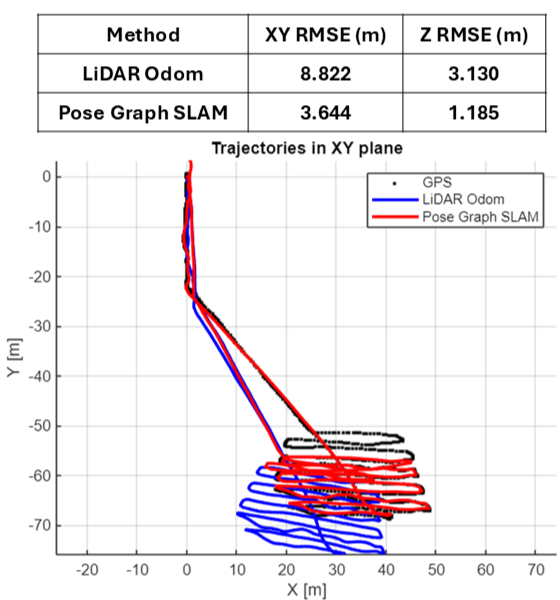
\includegraphics[width=\textwidth]{Included_Images/cov_0.04.png}
        \caption{Covariance Threshold = 0.04}
    \end{subfigure}
    \hfill
    \begin{subfigure}{0.45\textwidth}
        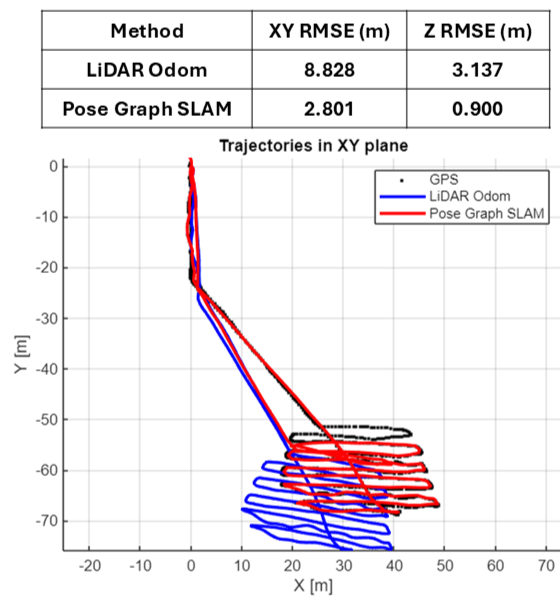
\includegraphics[width=\textwidth]{Included_Images/cov_0.1.png}
        \caption{Covariance Threshold = 0.1}
    \end{subfigure}
    \caption{Relationship between covariance threshold and Root Mean Square Error (RMSE) between pose graph SLAM trajectory and GPS trajectory.}
\end{figure}

Based on the Figure above, it is observed that the higher value of covariance threshold, the smaller the RMSE. This is because when more GPS data is being considered into the SLAM calculation, the total error score indicated in Equation \eqref{eq:error_score} will be used to correct the SLAM trajectory to the GPS trajectory.

Additionally, instead of observing a gradual convergence of the SLAM trajectory toward the GPS trajectory with the increase of covariance threshold, a distinct threshold value is identified at which the pose graph SLAM solution abruptly shifts from being dominated by LiDAR odometry to aligning closely with the GPS trajectory. This behavior occurs because the GPS covariance threshold is used to determine when the data begin to meaningfully influence the optimization. As shown in Figure \ref{fig:data1_cov}, the mean horizontal covariance of the GPS data is approximately 0.039$m^2$. This indicates that large portion of the GPS data cluster around this value. When the covariance threshold is set below 0.04, most GPS measurements are rejected for not meeting the required accuracy. On the other hand, once the covariance threshold exceeds this critical value, a large portion of GPS measurements becomes admissible to the optimization process. The sudden abundance of GPS data thus provide large influence on the total cost error, which is why there is a rapid jump on the SLAM trajectory towards the GPS trajectory.

\begin{figure} [H]
    \centering
    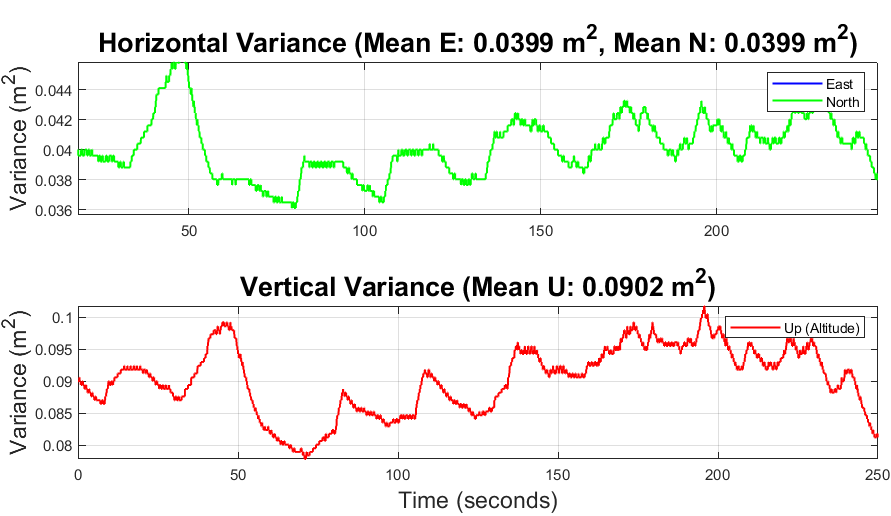
\includegraphics[width=0.6\textwidth]{Included_Images/data1_cov.png}
    \caption{Plot for GPS covariance in Data 2}
    \label{fig:data1_cov}
\end{figure}

However, the covariance (accuracy) of GPS is not consistent in different datasets as their accuracy varies continuously with environmental and system conditions \cite{vila2020survey}. In this case, the GPS covariance of all datasets are being plotted out to investigate the optimal covariance threshold for more versatile use cases. 

\begin{figure}[H]
    \centering
    \begin{subfigure}{0.49\textwidth}
        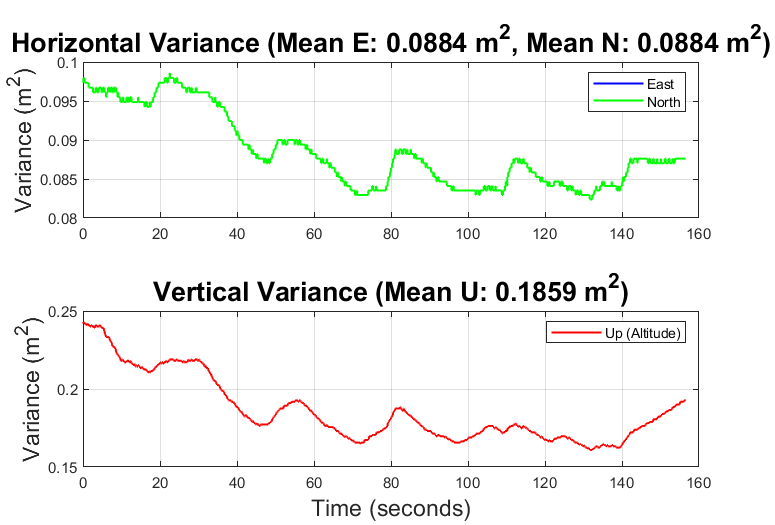
\includegraphics[width=\textwidth]{Included_Images/data5_cov.png}
        \caption{Data 3}
    \end{subfigure}
    \hfill
    \begin{subfigure}{0.49\textwidth}
        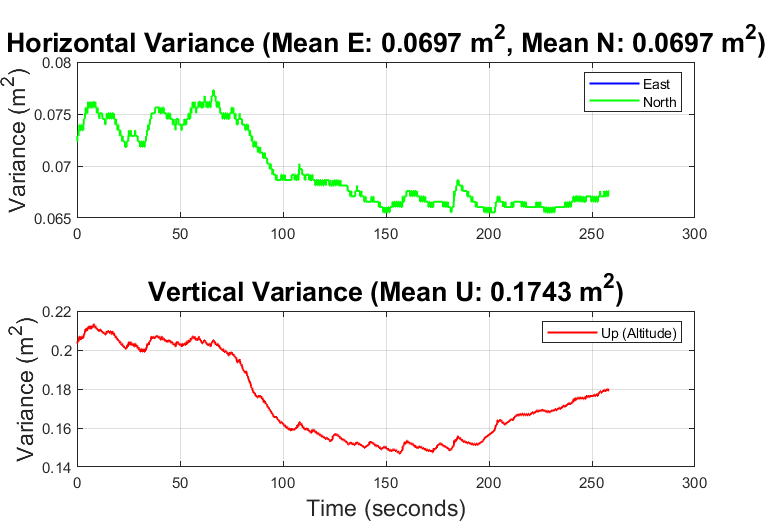
\includegraphics[width=\textwidth]{Included_Images/data7_cov.png}
        \caption{Data 4}
    \end{subfigure}
        \hfill
    \begin{subfigure}{0.49\textwidth}
        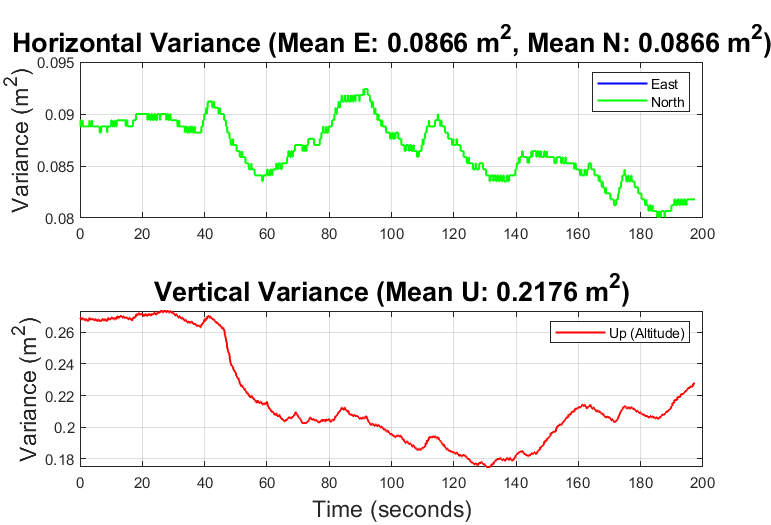
\includegraphics[width=\textwidth]{Included_Images/data8_cov.png}
        \caption{Data 5}
    \end{subfigure}
        \hfill
    \begin{subfigure}{0.49\textwidth}
        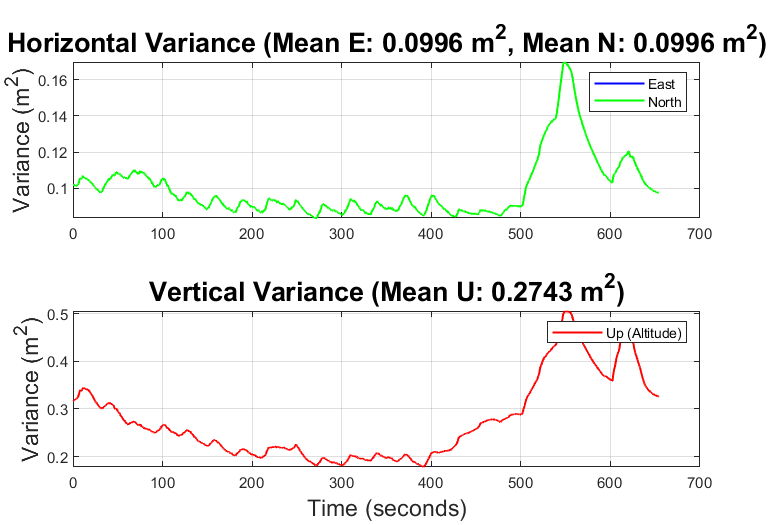
\includegraphics[width=\textwidth]{Included_Images/rosbag1_cov.png}
        \caption{Data 6}
    \end{subfigure}
    \caption{GPS covariance comparison from different dataset.}
\end{figure}

By referring to the mean covariance from all dataset, covariance threshold is set to 0.1 to allow SLAM system to trust the GPS measurement while avoiding large GPS noises being included. Figure below shows the point clouds and trajectory from the pose graph SLAM system with GPS incorporated. 

\begin{figure}[H]
    \centering
    \begin{subfigure}{0.45\textwidth}
        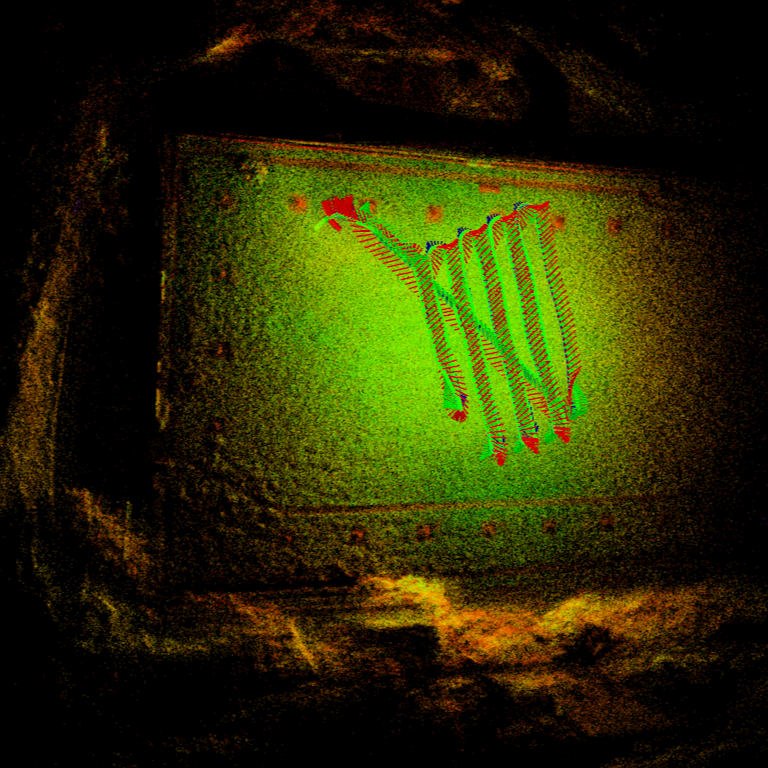
\includegraphics[width=\textwidth]{Included_Images/data5_pgo.png}
        \caption{Data 3}
    \end{subfigure}
    \hfill
    \begin{subfigure}{0.45\textwidth}
        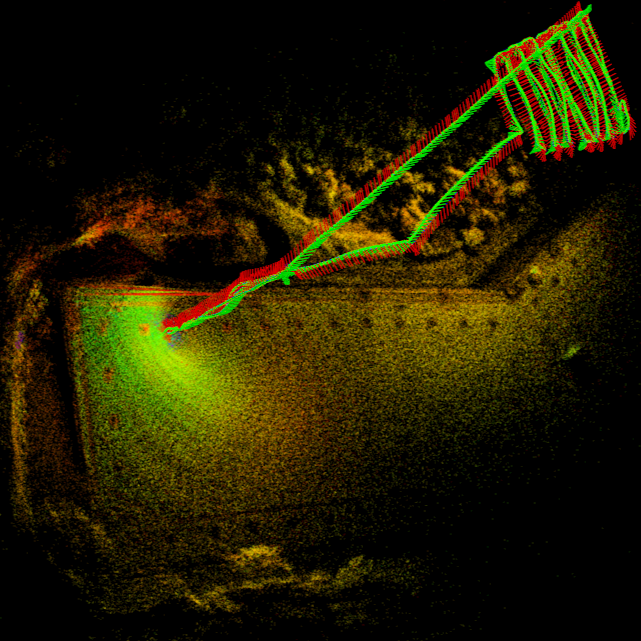
\includegraphics[width=\textwidth]{Included_Images/data7_pgo.png}
        \caption{Data 4}
    \end{subfigure}
        \hfill
    \begin{subfigure}{0.45\textwidth}
        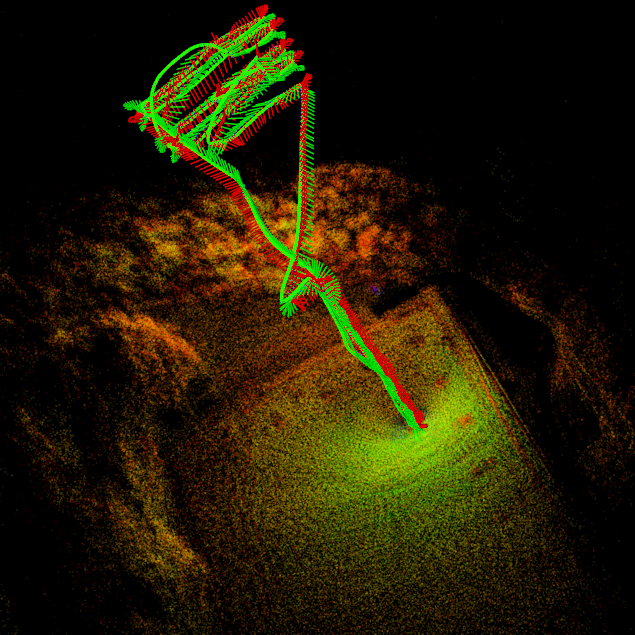
\includegraphics[width=\textwidth]{Included_Images/data8_pgo.png}
        \caption{Data 5}
    \end{subfigure}
        \hfill
    \begin{subfigure}{0.45\textwidth}
        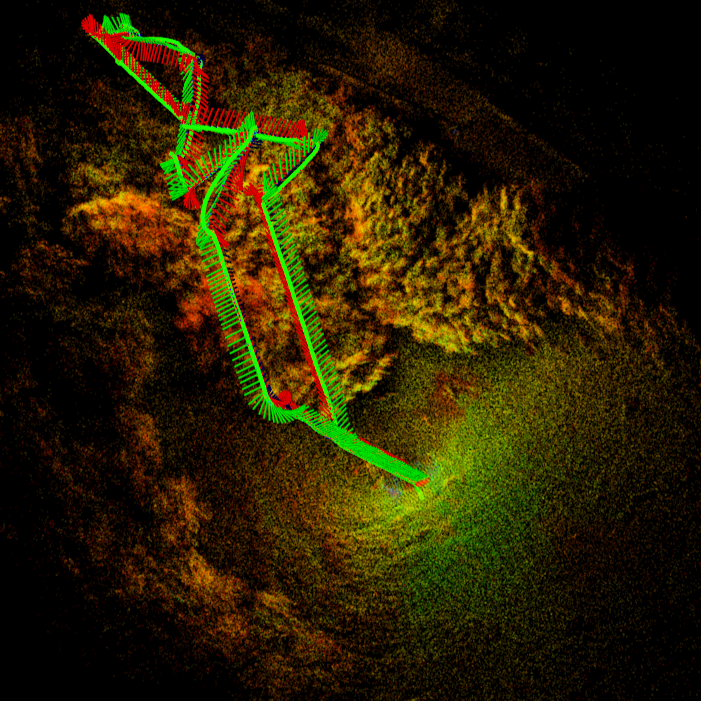
\includegraphics[width=\textwidth]{Included_Images/rosbag1_pgo.png}
        \caption{Data 6}
    \end{subfigure}
    \caption{Point cloud features and trajectories from pose graph SLAM with GPS.}
\end{figure}

With the combination of LiDAR odometry (Fast-LIO) and a pose graph SLAM system with GPS (PGO+GPS), distinct 3D point cloud features can be obtained in experimental areas where tree canopies and bare ground are well defined. In this case, the data can provide geometric reference for GNSS signals to cross validate whether the reflected signal from the satellite belongs to the ground, water surfaces, or tree canopies. 
\begin{figure}[H]
    \centering
    \begin{subfigure}{0.65\textwidth}
        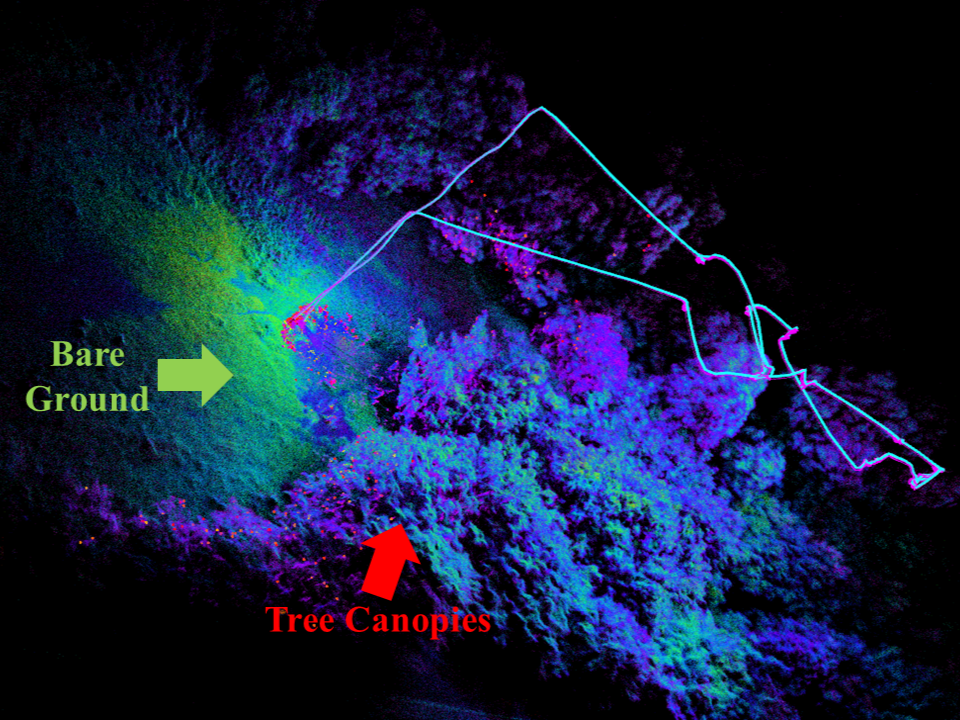
\includegraphics[width=\textwidth]{Included_Images/SLAM_anno_FL.png}
        \caption{Fast-LIO}
    \end{subfigure}
    \par\medskip
    \begin{subfigure}{0.65\textwidth}
        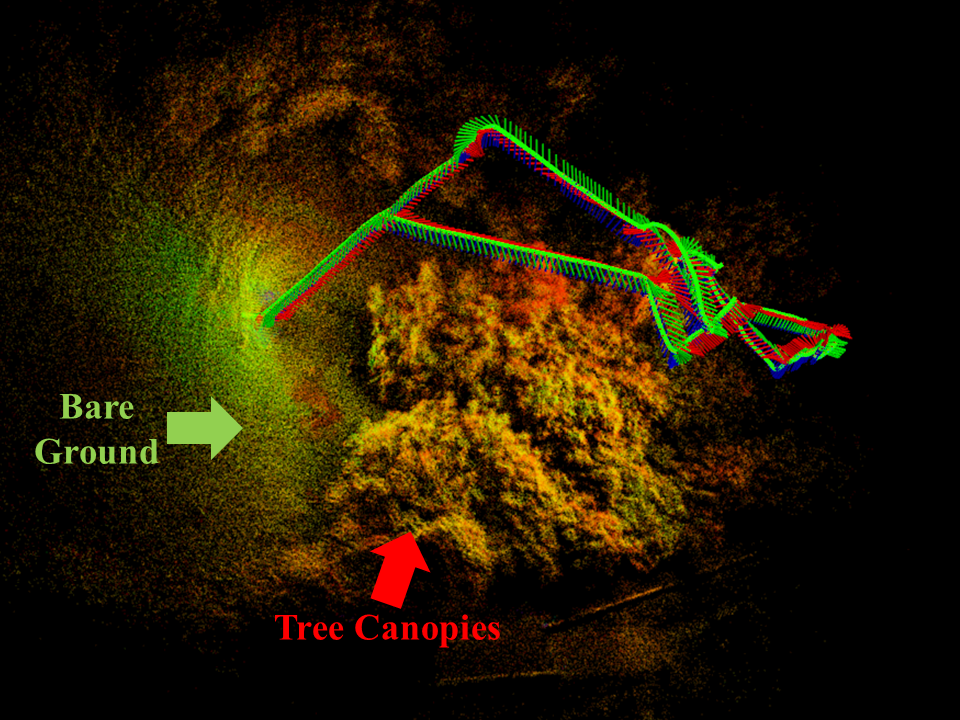
\includegraphics[width=\textwidth]{Included_Images/SLAM_anno_pgo.png}
        \caption{PGO+GPS}
    \end{subfigure}
    \caption{Odometry and pose graph SLAM results that capture distinguish features such as bare ground and tree canopies.}
\end{figure}


\subsubsection{Limitations}
Although the incorporation of GPS provides global constraints that enable the SLAM system to correct and align its trajectory, this correction is not always applied. If the SLAM trajectory deviates significantly from the GPS trajectory, the system will not consider the GPS data in the SLAM optimization. This can be observed in Figure \ref{fig:pgo_drift}, where the SLAM trajectory drifts due to accumulated errors from LiDAR odometry. In the figure, the GPS measurements remain in their correct global positions, while the SLAM trajectory continues to follow the drifted path.

\begin{figure}[H]
    \centering
    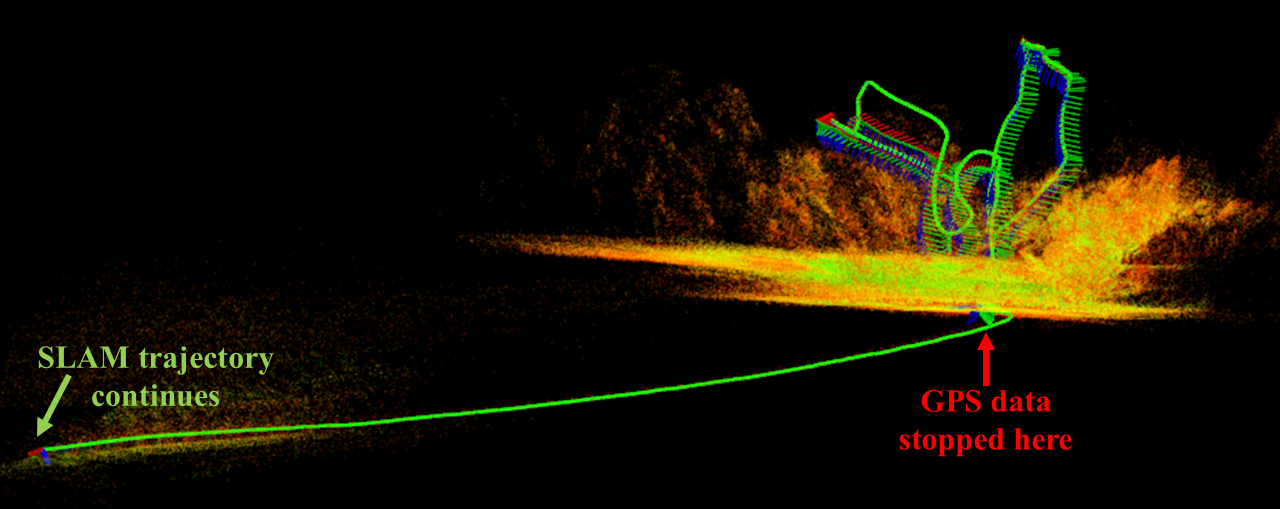
\includegraphics[width=0.9\textwidth]{Included_Images/pgo_drift.png}
    \caption{Pose graph SLAM system with drifted trajectory.}
    \label{fig:pgo_drift}
\end{figure}

This occurs because the pose graph SLAM framework consist of mathematical outlier rejection mechanisms that evaluate the residual between the LiDAR odometry estimates and the GPS measurements. If the distance grows unusually large between both sensors, the GPS measurements are classified as outliers and excluded from the optimization process. As a result, GPS data is not used to correct the trajectory in cases of significant odometry drift.

% --- GNSS-R ---
\section{GNSS-R}

\subsection{Literature Review}
The concept of GNSS-R for remote sensing applications was first proposed in
1993, where the correlation between direct and scattered GNSS signals was proven
promising for ocean altimetry \cite{MartnNeira1993APR}. Today, apart from the
originally proposed application, GNSS-R techniques have been extensively used
for Earth observations and land information retrieval, including ocean salinity,
soil moisture, and ice thickness \cite{RodriguezAlvarez2011}. However, research
on vegetation parameter retrieval remains limited to preliminary analyses
\cite{Jia2018}. 

In a previous study, the capabilities of monitoring vegetation through GNSS-R
were demonstrated through a theoretical simulation of GNSS scattering
characteristics \cite{Ferrazzoli2011}. Furthermore, this study revealed that the
sensitivity of GNSS-R signals can be influenced by incidence angle, soil
parameters, and tree size, while signals with lower elevation angles and RL
polarization (transmission of right-hand circular polarized (RHCP) signal,
reception of left-hand circular polarized (LHCP) signal) appeared to be ideal
for forest monitoring \cite{Ferrazzoli2011}. As GNSS signals are natively
transmitted in RHCP, no modification on the transmitter is necessary for
practical forest monitoring applications. However, since GNSS signals flip to
LHCP upon reflection, a receiver capable of receiving LHCP signals is necessary
to complete the RL polarization configuration \cite{Jia2018}. In another study,
the polarization scattering properties of GNSS-R signals in forest canopies were
modelled, where simulations revealed that tree trunk scattering effects would
dominate total scattering response, while satellite azimuth angles are
significantly correlated to the signal polarization \cite{Wu2014}. 

Aside from simulated approaches, empirical or semi-empirical studies regarding
GNSS-R remote sensing of vegetation were also reviewed. In a study by Yueh et
al., GNSS-R data onboard the Cyclone GNSS (CYGNSS) satellite were analyzed
against the vegetation water content estimated through the satellite-derived
Normalized Difference Vegetation Index (NDVI) \cite{Yueh2022}. The results
demonstrated near-linear relationship between vegetation water content and
GNSS-R signal attenuation, while the CYGNSS data also suggested the existence of
signal scattering effects within complex forest components \cite{Yueh2022}.
Similarly, another study analyzing GNSS-R data from TechDemoSat-1 demonstrated
reduced sensitivity to soil moisture retrieval due to vegetation attenuation,
which could be effectively compensated using NDVI data, indicating a correlation
between signal attenuation and vegetation water content \cite{Camps2016}.
Additionally, the interference pattern between direct and reflected GNSS signals
from the Earth's surface was used in estimating vegetation height and land
topography \cite{RodriguezAlvarez2011}. Using a Soil Moisture
Interference-pattern GNSS Observations at L-band (SMIGOL) reflectometer, which
receives both the direct and reflected signals simultaneously, the power of the
received signals was coherently added. As a result, the recorded power
oscillations due to interference present notches that are correlated to
vegetation layer thickness and the reflection geometry (Figure \ref{SMIGOL})
\cite{RodriguezAlvarez2011}. Ultimately, a Root Mean Square Error (RMSE) of 3-5
cm in estimating the height of vegetation with simple geometrical structures
(barley and wheat) could be achieved \cite{RodriguezAlvarez2011}.

\begin{figure}[H]
    \centering
    \begin{subfigure}{0.49\textwidth}
        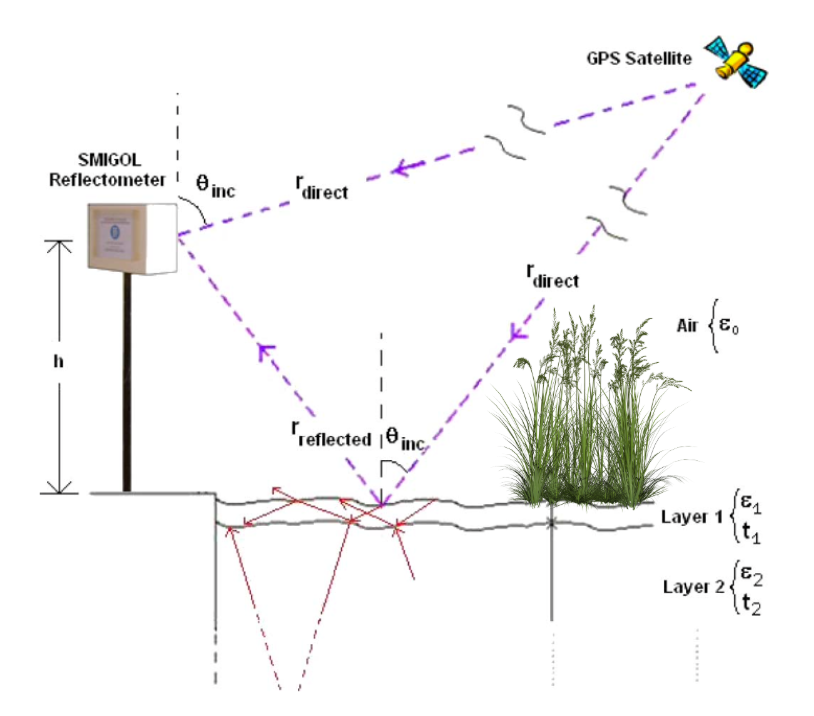
\includegraphics[width=0.8\textwidth]{Included_Images/SMIGOL_reflectometer.png}
        \caption{SMIGOL Reflectometer Setup}
    \end{subfigure}
    \hfill
    \begin{subfigure}{0.49\textwidth}
        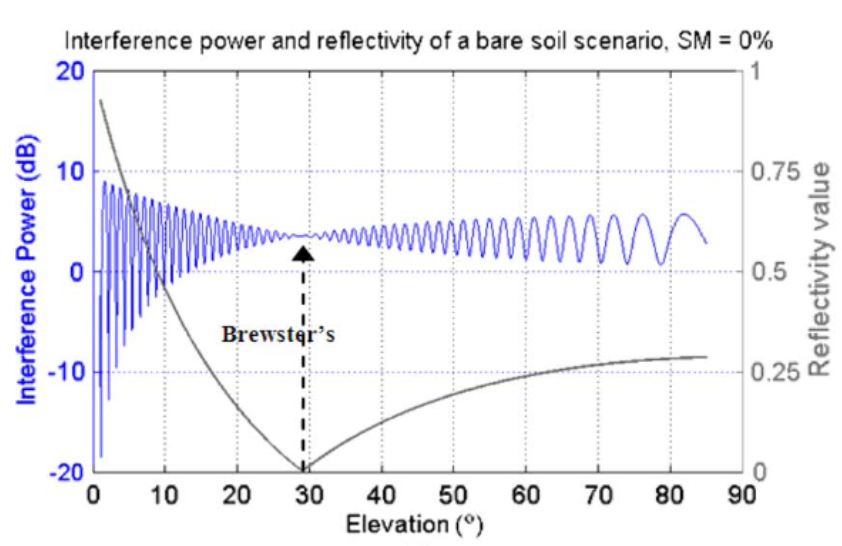
\includegraphics[width=\textwidth]{Included_Images/SMIGOL_interference.png}
        \caption{Interference Notch}
    \end{subfigure}
    \caption{Setup and interference notch examples of the SMIGOL reflectometer
    \cite{RodriguezAlvarez2011}.}
    \label{SMIGOL}
\end{figure}

The following table summarizes several contemporary research on GNSS-R remote sensing:

\begin{table}[H]
    \centering
    \caption{Contemporary GNSS-R Research in Vegetation Monitoring}
    \begin{tabularx}{\linewidth}{@{} l X @{}}
    \toprule
    \textbf{Study} & \textbf{Key Findings} \\
    \midrule
    Ferrazzoli et al. (2011) & GNSS-R signals are sensitive to incidence angle,
    soil parameters, and tree size, with RL polarization being ideal for forest
    monitoring. \\
    \midrule
    Rodríguez-Álvarez et al. (2011) & A SMIGOL reflectometer can be used to
    achieve 3-5 cm RMSE in estimating simple vegetation height. \\
    \midrule
    Wu et al. (2014) & Tree trunk scattering effects dominate the total GNSS-R
    response, while satellite azimuth angles are correlated to signal
    polarization. \\
    \midrule
    Camps et al. (2016) & Vegetation attenuation of GNSS-R signals reduces soil
    moisture retrieval sensitivity, but this effect can be effectively
    compensated using NDVI data, indicating a correlation. \\
    \midrule
    Yueh et al. (2022) & CYGNSS data demonstrates linear relationship between
    vegetation water content and GNSS-R signal attenuation. \\
    \bottomrule
    \end{tabularx}
\end{table}

Yet, despite the effort in prior studies, the use of GNSS-R techniques in
vegetation remote sensing and monitoring is far from developed. Most
importantly, existing research relies heavily on space-borne or static
ground-based platforms, while the use of high spatial resolution and high
flexibility platforms - such as a UAV - remains underexplored. Therefore, it is
critical to develop a systematic framework for a UAV-based GNSS-R system, in
which correlations between GNSS-R signal features and vegetation condition
parameters are comprehensively assessed and modelled.

\subsection{Methodology}
In this project, a RL polarization system is adopted, where the UAV is equipped with two antennas:

\begin{figure}[H]
    \centering
    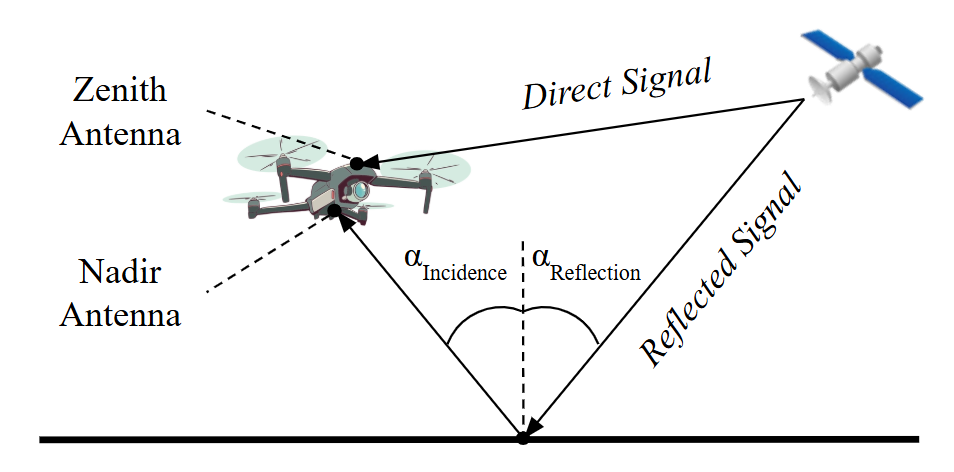
\includegraphics[width=0.75\textwidth]{Included_Images/RL_system.png}
    \caption{RL polarization system adopted for this project.}
\end{figure}

Here, the zenith antenna receives the RHCP signals that propagate in a straight
line from the satellite to the UAV, while the nadir antenna receives the LHCP
signals that have reflected off the ground. A schematic representation of the
two types of GNSS signal polarization are shown in Figure
\ref{GNSS_polarization} below. By comparing the characteristic differences
between the direct and the reflected signals, the influence of ground features
on the reflected signal can be inferred, analyzed, and modelled. 

\begin{figure}[H]
    \begin{subfigure}{0.49\textwidth}
        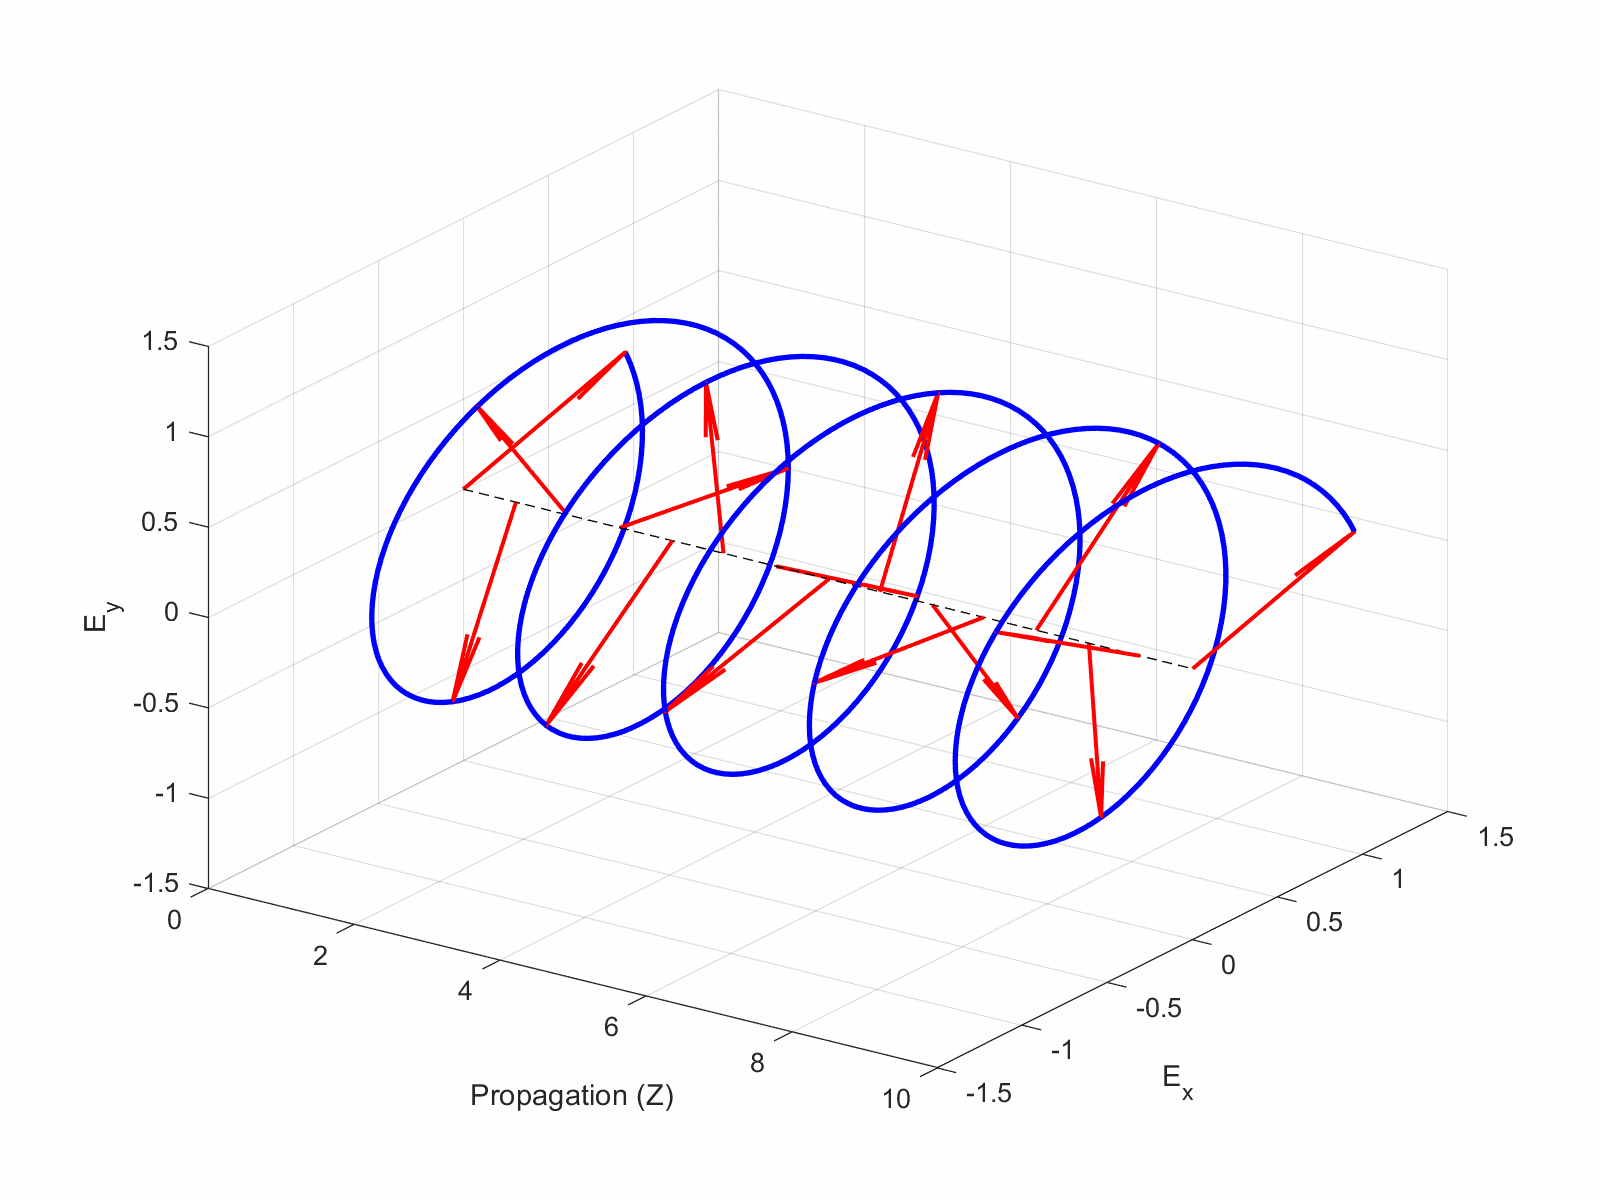
\includegraphics[width=\textwidth]{Included_Images/RHCP.png}
        \caption{Right-Hand Circular Polarization \\ (Direct GNSS Signal)}
    \end{subfigure}
    \hfill
    \begin{subfigure}{0.49\textwidth}
        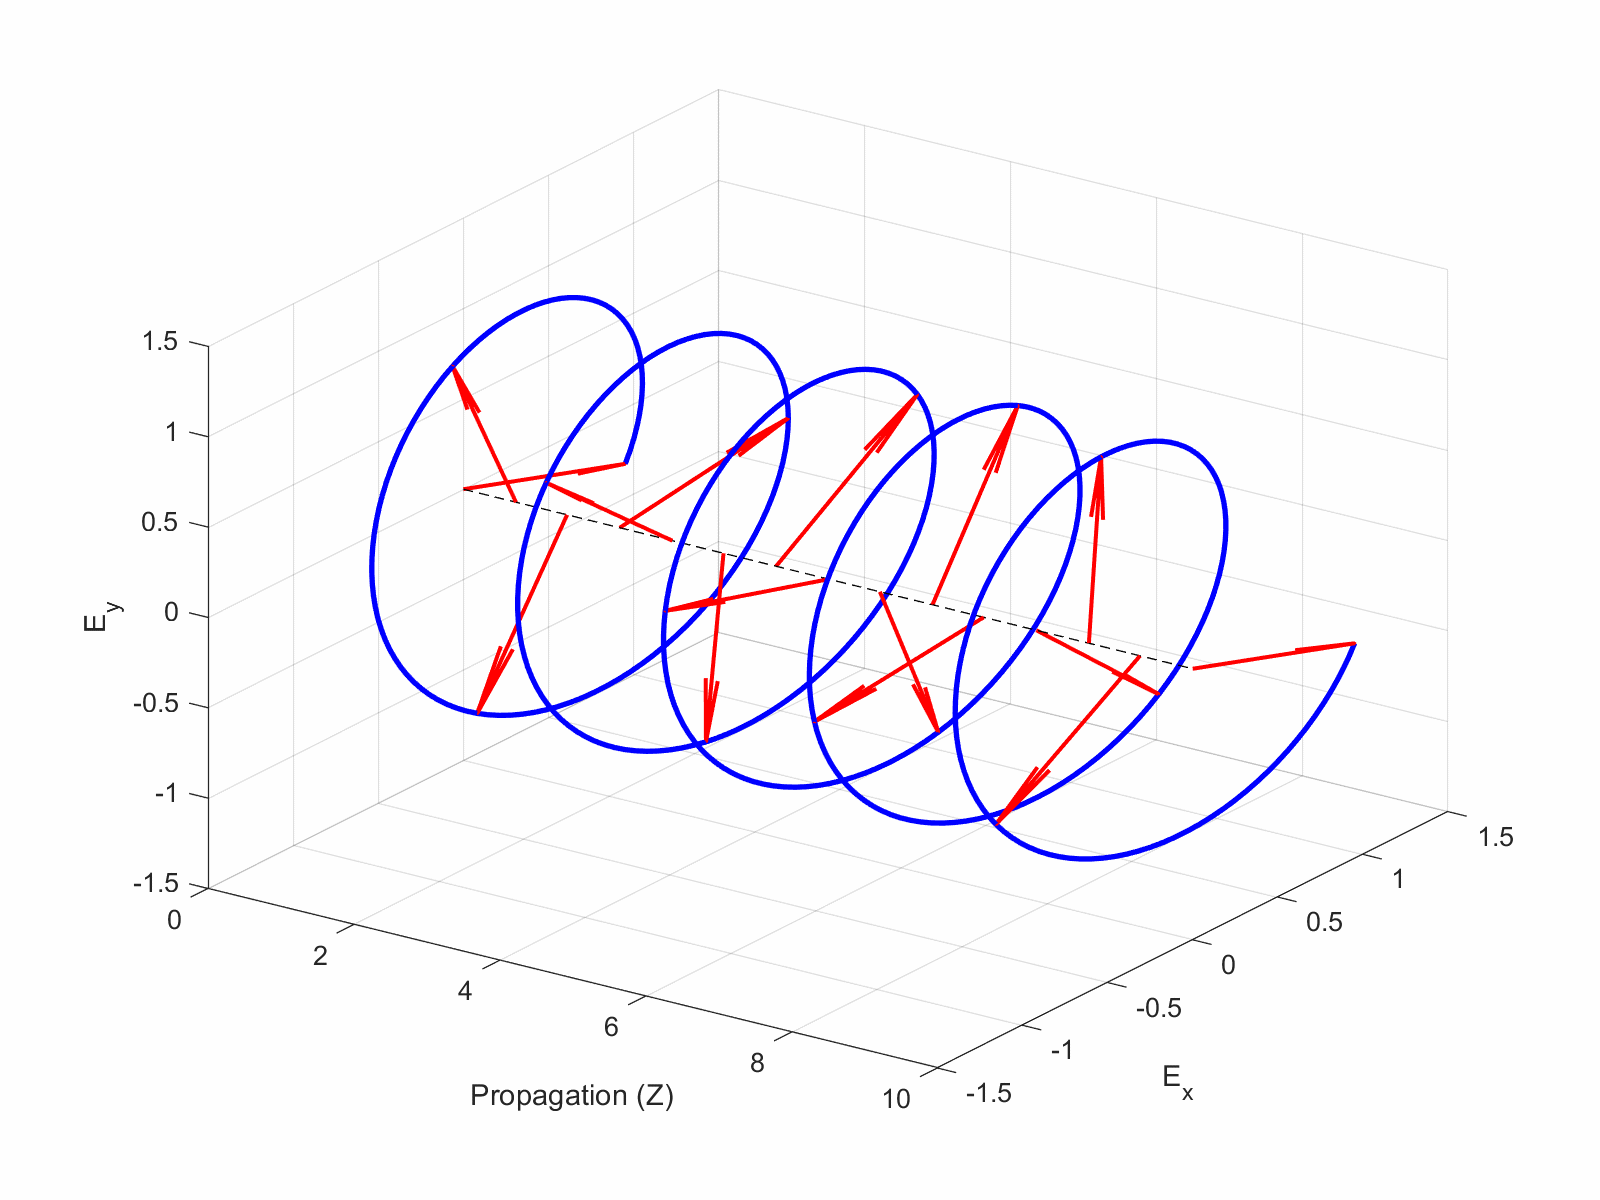
\includegraphics[width=\textwidth]{Included_Images/LHCP.png}
        \caption{Left-Hand Circular Polarization \\ (Reflected GNSS Signal)}
    \end{subfigure}
    \caption{Two GNSS signal polarization types within the RL polarization System.}
    \label{GNSS_polarization}
\end{figure}

First, raw GNSS data collected from both receivers during the flights are
processed to extract key GNSS measurements. Then, the location and geometry of
the First Fresnel Zone (FFZ) of reflection are calculated for each reflected
signal, while the characteristics of the GNSS measurements are analyzed with
respect to any ground features that fall within the FFZ. Finally, the
correlation between GNSS measurement features and ground features are
systematically summarized and modelled. The following sections detail the GNSS
measurement retrieval process, the calculation of FFZ location and geometry, as
well as the quantitative modelling of correlations between GNSS parameters and
ground features. Additionally, the open-source code repository developed for the
GNSS-R framework of this project is presented in the Appendix.

\subsubsection{GNSS Measurement Extraction}
Two raw data sources are necessary for the extraction of key GNSS measurements
used for GNSS-R: the raw binary GNSS data and the Pixhawk controller log. First,
the binary GNSS data is converted into readable observation files using RTKCONV
\cite{takasu2009rtklib}, and together with the satellite ephemeris data
downloaded from \url{https://cddis.nasa.gov/archive/gnss/data/}, measurements
such as the satellite elevation angle, pseudorange, and carrier to noise ratio
could be extracted using the MatRTKLIB library \cite{taroz:matrtklib}. From the
Pixhawk controller log, the UAV position, which is a filtered positioning result
from onboard sensor inputs, is obtained and regarded as the ground truth
assuming that the positioning error is small. Then, two key GNSS measurement
parameters are calculated for correlation analysis against ground features:
carrier to noise ratio and excess pseudorange delay. 

\begin{figure}[H]
    \centering
    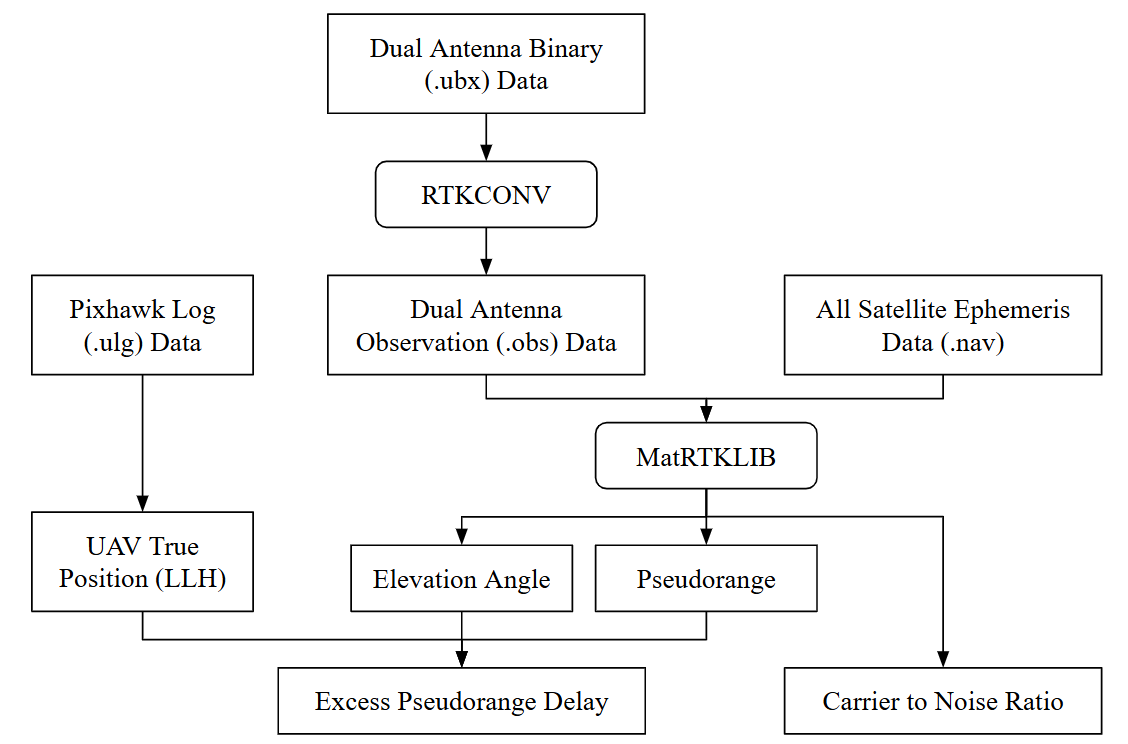
\includegraphics[width=0.85\textwidth]{Included_Images/GNSS_Measurement_Flow.png}
    \caption{Workflow of extracting GNSS measurements from raw data.}
\end{figure}

\paragraph{Carrier to Noise Ratio} ~\\
Carrier to noise ratio ($C/N_0$) refers to the power of received carrier signal
relative to the noise power per unit bandwidth, usually with a unit of
decibel-Hertz (dB-Hz) \cite{joseph2010gnss}. $C/N_0$ can be readily obtained
from the receiver, and it is calculated as the following:
\begin{equation}
    C/N_0 = C - (N - BW)
\end{equation}
where $C$ refers to the carrier power in dBm or dBW; $N$ refers to the noise
power in dBm or dBW; and $BW$ refers to the bandwidth of the signal in Hz. Since
a signal's $C/N_0$ can be attenuated by scattering off from trees or reflecting
off from the ground, the attenuation profiles from different ground objects may
carry key information that describe potential ground features. 

\paragraph{Excess Pseudorange Delay} ~\\
In GNSS, pseudorange refers to the "apparent" distance between a satellite and a
receiver, which includes the true geometric separation between the satellite and
the receiver, plus various biases and delays. For a signal that directly
propagates from a satellite to the zenith antenna along a straight path, its
pseudorange $\rho_{direct}$ can be expressed as the following
\cite{kaplan2017understanding}:
\begin{equation}
    \rho_{direct} = R_{direct} + \Delta t_{zenith} + \Delta t_s + I + T
\end{equation}
where $R_{direct}$ refers to the true geometric distance between the satellite
and the receiver; $\Delta t_{zenith}$ refers to the zenith receiver clock bias;
$\Delta t_s$ refers to the satellite clock bias; $I$ refers to the ionospheric
delay; and $T$ refers to the tropospheric delay. \\
On the other hand, for a signal that have reflected off the ground and received
by the nadir antenna, its pseudorange $\rho_{reflected}$ can be expressed using
a similar equation with two additional error terms:
\begin{equation}
    \rho_{reflected} = R_{direct} + \Delta t_{nadir} + \Delta t_s + I + T + E_{reflection} + \epsilon
\end{equation}
where $\Delta t_{nadir}$ refers to the nadir receiver clock bias;
$E_{reflection}$ refers to the path delay caused by geometric reflection; and
$\epsilon$ refers to the excess pseudorange delay, which accounts for unmodelled
errors such as scattering from vegetation. A diagram illustrating the direct and
the reflected signal's propagation path is shown in Figure \ref{Excess
Pseudorange Delay Diagram} below.
\begin{figure}[H]
    \centering
    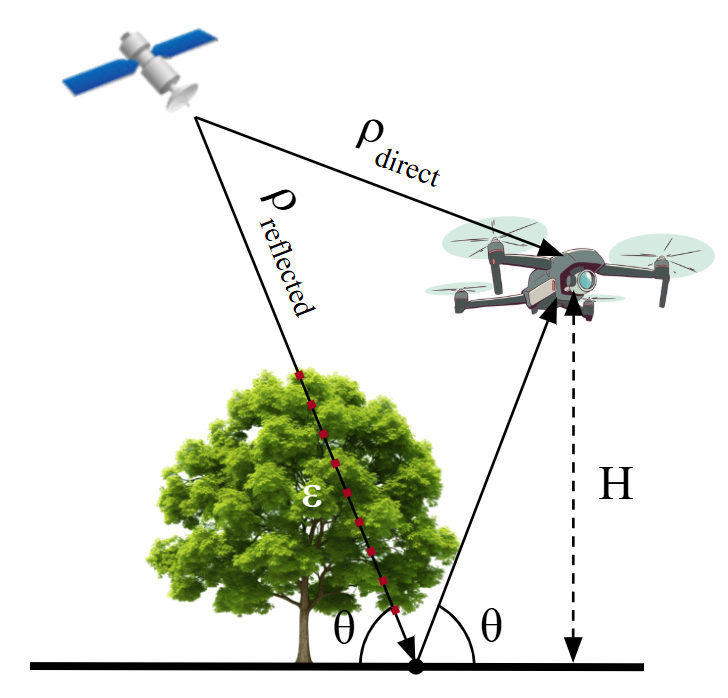
\includegraphics[width=0.5\textwidth]{Included_Images/excess_pseudorange_delay.png}
    \caption{Propagation paths of the direct and the reflected signal in the adopted GNSS-R system.}
    \label{Excess Pseudorange Delay Diagram}
\end{figure}
Since the satellite is significantly further away from the UAV compared to the
point of reflection on ground, the path delay caused by geometric reflection,
$E_{reflection}$, could be calculated using the following expression:
\begin{equation}
    E_{reflection} = \frac{2H}{sin(\theta)}
\end{equation}
where $\theta$ refers to the satellite's elevation angle and $H$ refers to the
UAV's above ground altitude. Here, since the UAV's true position is given in the
global coordinate of latitude, longitude, and height (LLH) in the Pixhawk log
data, the terrain height shall be subtracted from the given ellipsoidal height
to obtain the above ground altitude, $H$. This terrain height is obtained
through the Hong Kong Digital Terrain Model
(\url{https://data.gov.hk/en-data/dataset/hk-landsd-openmap-5m-grid-dtm}), which
provides the topographical information in 5 meter by 5 meter grids with an
accuracy of $\pm$ 5 meters \cite{dataDigitalTerrain}. \\
Substituting $E_{reflection}$ into the pseudorange equation of the reflected
signal while taking the difference between the direct signal and the reflected
signal's pseudoranges, the true geometric distance between the satellite and the
receivers ($R_{direct}$), satellite clock bias ($\Delta t_s$), ionospheric delay
($I$), and tropospheric delay ($T$) can be effectively cancelled: 
\begin{equation}
    \rho_{reflected} - \rho_{direct} = \Delta t_{nadir} - \Delta t_{zenith} + \frac{2H}{sin(\theta)} + \epsilon
\end{equation}
while the difference between the receiver clock biases, $\Delta t_{nadir} -
\Delta t_{zenith}$, can be approximated as the mean of the residual
pseudorange difference after compensating for the reflection delay:
\begin{equation}
    \Delta t_{nadir} - \Delta t_{zenith} \approx \frac{\sum_{i=1}^{n}(\rho_{reflected}^{i} - \rho_{direct}^{i} - \frac{2H}{sin(\theta^{i})})}{n}
\end{equation}
where $n$ refers to the number of satellites received by both zenith and nadir
antenna at a given epoch. This approximation is valid because the residual
pseudorange difference after removing the geometric reflection delay follows a
normal distribution, as shown in Figure \ref{pr_diff-reflection_delay}, hence
its mean provides the most likely value for the relatively constant hardware
clock bias. 
\begin{figure}[H]
    \centering
    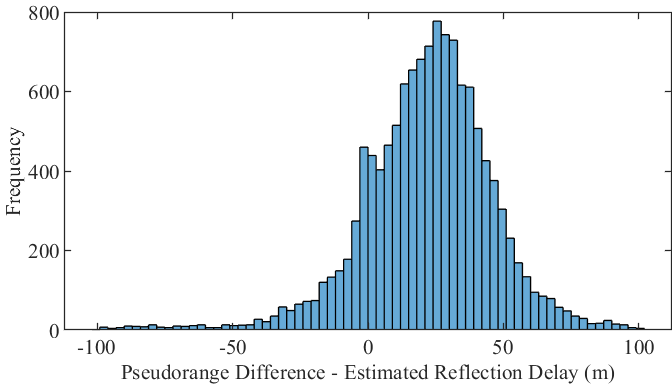
\includegraphics[width=0.75\textwidth]{Included_Images/pr_diff-reflection_delay.png}
    \caption{Distribution of the residual pseudorange difference after removing the geometric reflection delay.}
    \label{pr_diff-reflection_delay}
\end{figure}
Lastly, the excess pseudorange delay can be calculated:
\begin{equation}
    \epsilon = \rho_{reflected} - \rho_{direct} - (\Delta t_{nadir} - \Delta t_{zenith}) - \frac{2H}{sin(\theta)}
\end{equation}
where its value may carry key information that describes the interaction
between the reflected signals and various ground features.

\subsubsection{First Fresnel Zone Calculation}
\label{sec:first_fresnel_zone_calculation}
Following the extraction of GNSS measurements observed onboard the UAV, the GNSS
signals are particularly analyzed with respect to the 2-dimensional ground
regions that they reflect off from.

\begin{figure}[H]
    \centering
    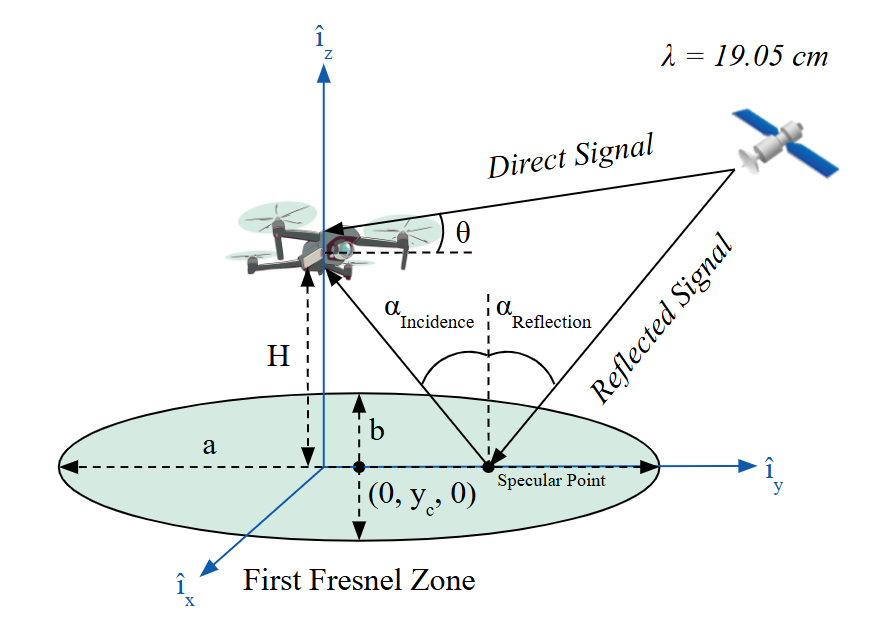
\includegraphics[width=0.8\textwidth]{Included_Images/Fresnel_Zone_Illustration.png}
    \caption{Schematic diagram of GNSS-R signal reflection geometry with the First Fresnel Zone illustrated.}
\end{figure}

Within this region, a specular reflection point could be found, where the angle
of incidence is equal to the angle of reflection. The primary scattering area
around the specular point in which reflected signals arrive at the receiver in
coherence is called the First Fresnel Zone (FFZ). By definition, it is an
ellipse for which the signal phase change across is within $\frac{\lambda}{2}$
radians, where $\lambda$ refers to the signal wavelength \cite{Jia2018}. Given
the satellite elevation angle $\theta$ and the UAV's above ground altitude $H$,
the semi-major axis $a$ and the semi-minor axis $b$ of the FFZ can be calculated
as the following \cite{yu2021theory}: 

\begin{equation}
    a = \frac{\sqrt{\lambda H sin(\theta)+\frac{\lambda^2}{4}}}{(sin(\theta))^2}
\end{equation}

\begin{equation}
    b = \frac{\sqrt{\lambda H sin(\theta)+\frac{\lambda^2}{4}}}{sin(\theta)}
\end{equation}

To calculate the location of the FFZ center, a local coordinate system is
defined. The UAV's ground projection acts as the coordinate origin, while the
y-axis aligns with the ground projection of the vector from the UAV to the
satellite. The z-axis follows the up direction of the local East-North-Up (ENU)
coordinates, and the x-axis completes the coordinate system by remaining
orthogonal to both x and y axes. In this coordinate system, the location of the
FFZ center could be expressed as $(x_c, y_c, z_c)$, where \cite{yu2021theory}:

\begin{equation}
    x_c = 0
\end{equation}
\begin{equation}
    y_c = (\frac{\lambda}{2}+ H sin(\theta))\frac{cos(\theta)}{(sin(\theta))^2}
\end{equation}
\begin{equation}
    z_c = 0
\end{equation}

\subsubsection{Correlation Modelling}
After obtaining each received signal's $C/N_0$ ratio and excess pseudorange
delay, any correlation between the GNSS measurement parameters and ground
features within the FFZs are qualitatively analyzed and quantitatively
modelled. To model the correlations quantitatively, the aerial
Color-Infrared (CIR) image from the Hong Kong Lands Department
(\url{https://www.landsd.gov.hk/en/survey-mapping/mapping/aerial-photo-photogrammetric-products/digital-aerial-photo.html})
is used as the ground truth for quantifying ground features.

\begin{figure}[H]
    \centering
    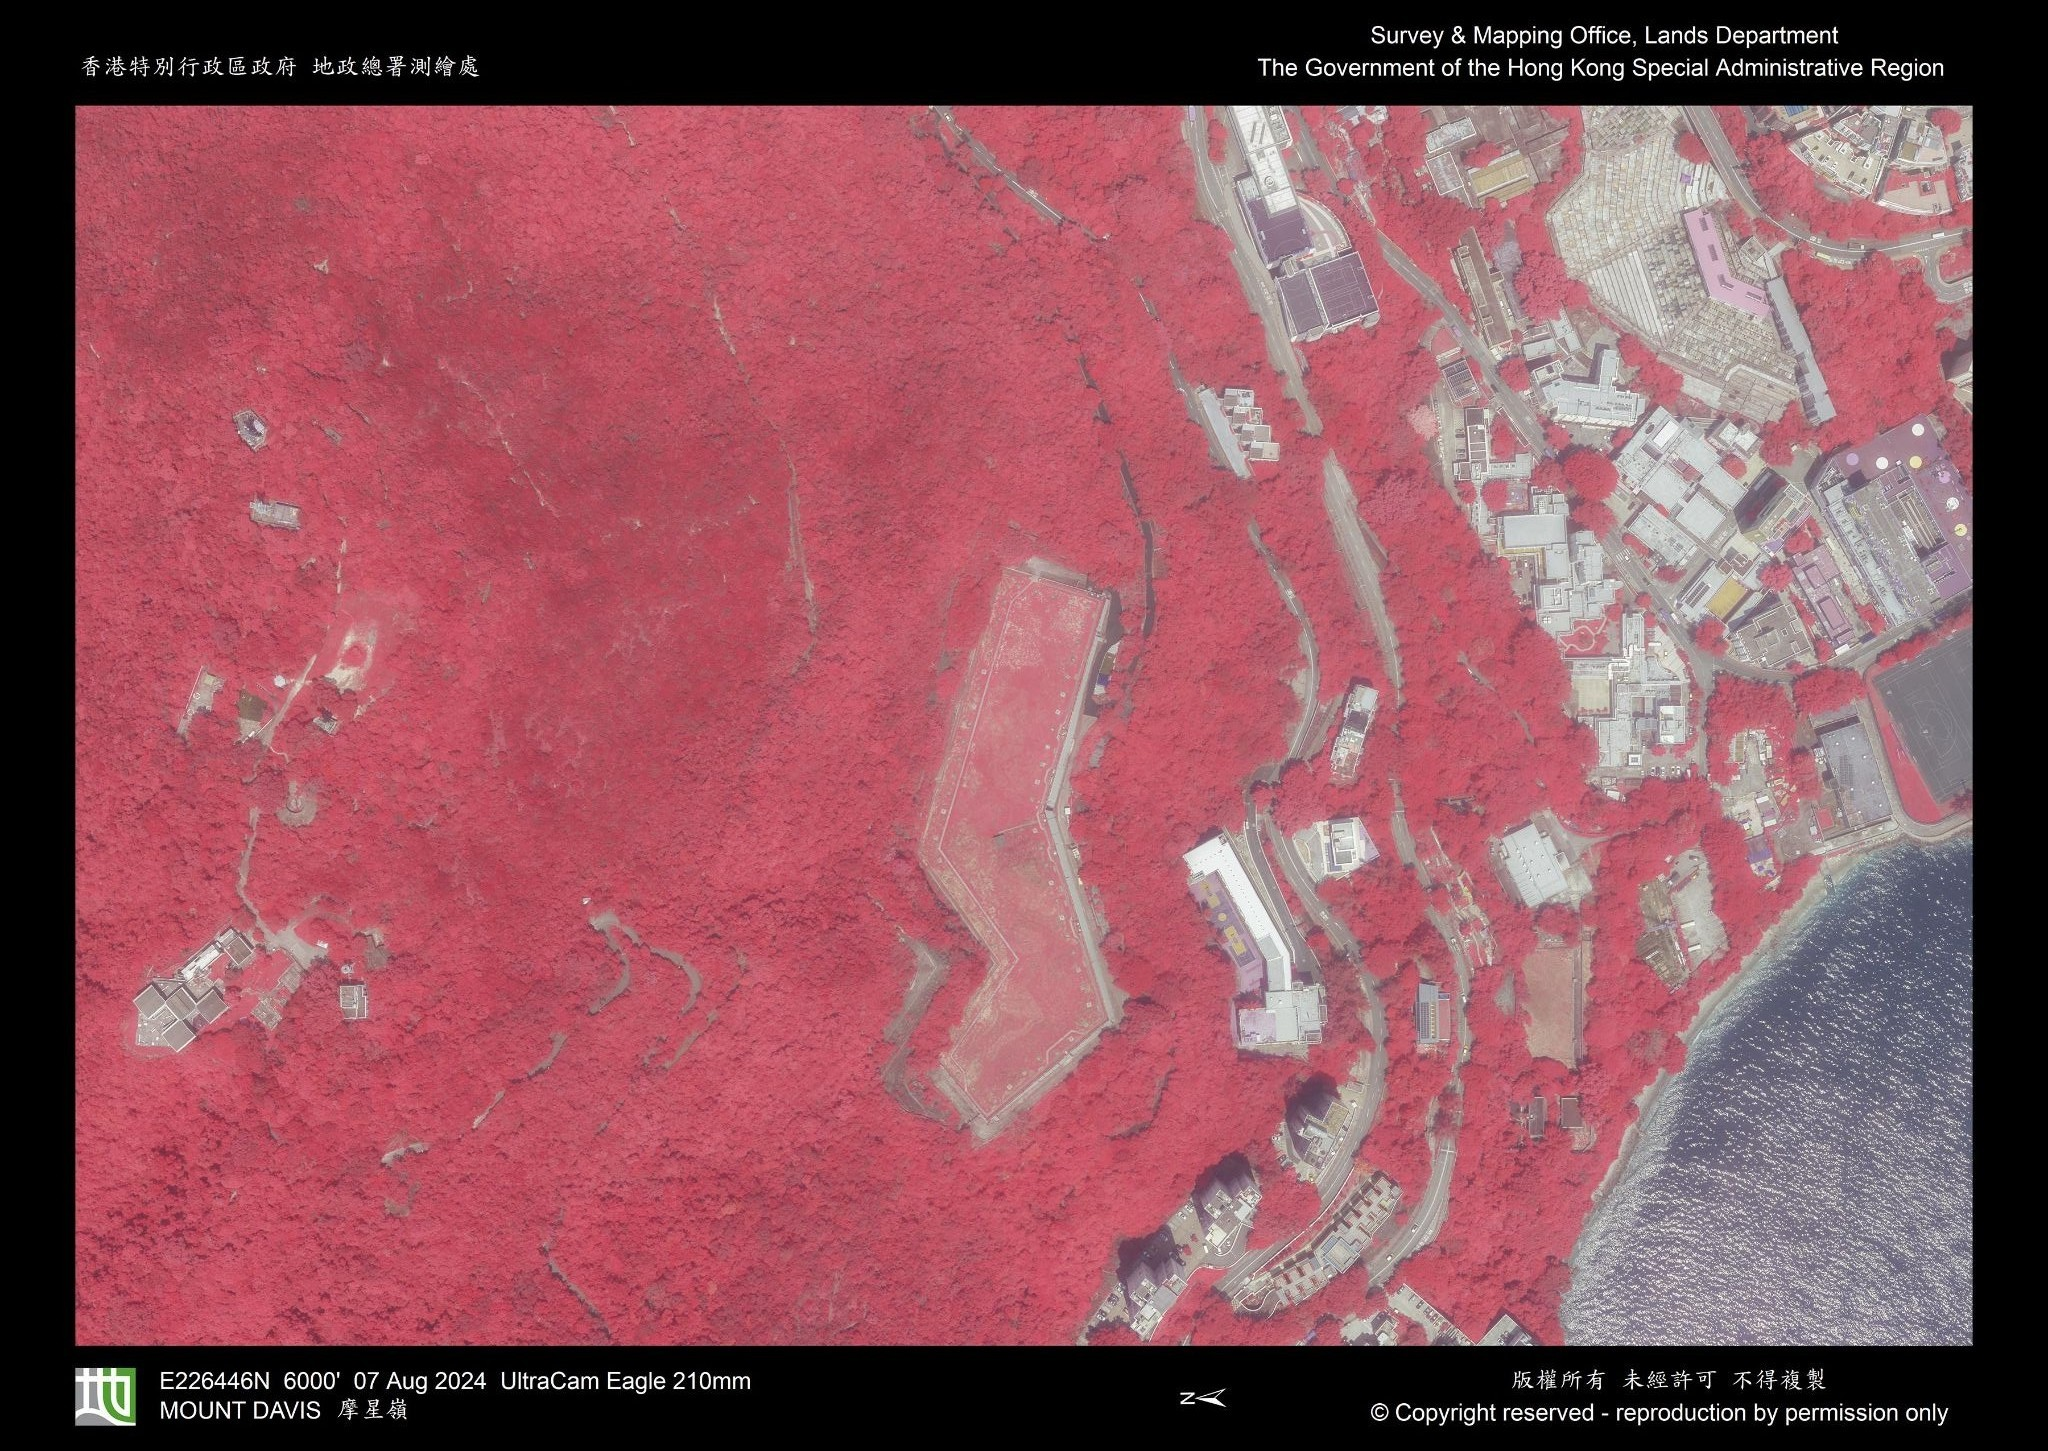
\includegraphics[width=0.8\textwidth]{Included_Images/example_CIR_image.jpg}
    \caption{An example of the aerial CIR image obtained from the Lands Department \cite{HKLandsD_CIR_2024}.}
\end{figure}

CIR image is a common remote sensing tool used to display vegetation health,
where the visible color spectrum of each image is shifted rightward to display
the infrared radiation invisible to the human eye
\cite{campbell2011introduction}. Particularly, the infrared radiation from
vegetation (which is displayed as red) is correlated to their chlorophyll
content, where a vibrant red indicates dense vegetation while lighter reds
indicate sparse vegetation. Additionally, bare soil tends to appear tan while
water surfaces tend to appear black on CIR images.

\begin{figure}[H]
    \centering
    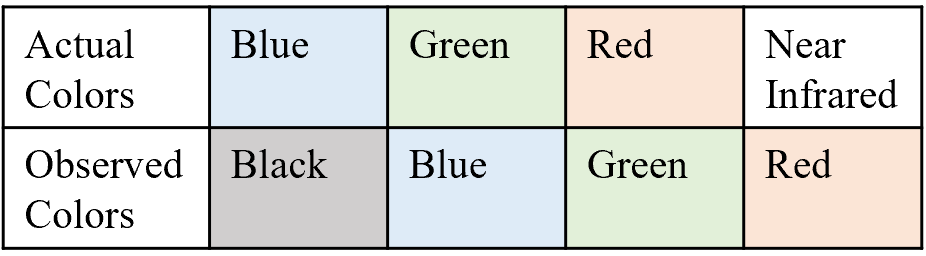
\includegraphics[width=0.5\textwidth]{Included_Images/CIR_spectrum.png}
    \caption{Actual colors vs the observed colors on a CIR image.}
\end{figure}

To leverage CIR images for extracting ground features, they are first
geo-referenced to match each image pixel to its corresponding longitude and
latitude. This could be done through a projective transformation using the
corner coordinates provided by the Lands Department, as illustrated in Figure
\ref{CIR Georeference} below. 

\begin{figure}[H]
    \begin{subfigure}{0.49\textwidth}
        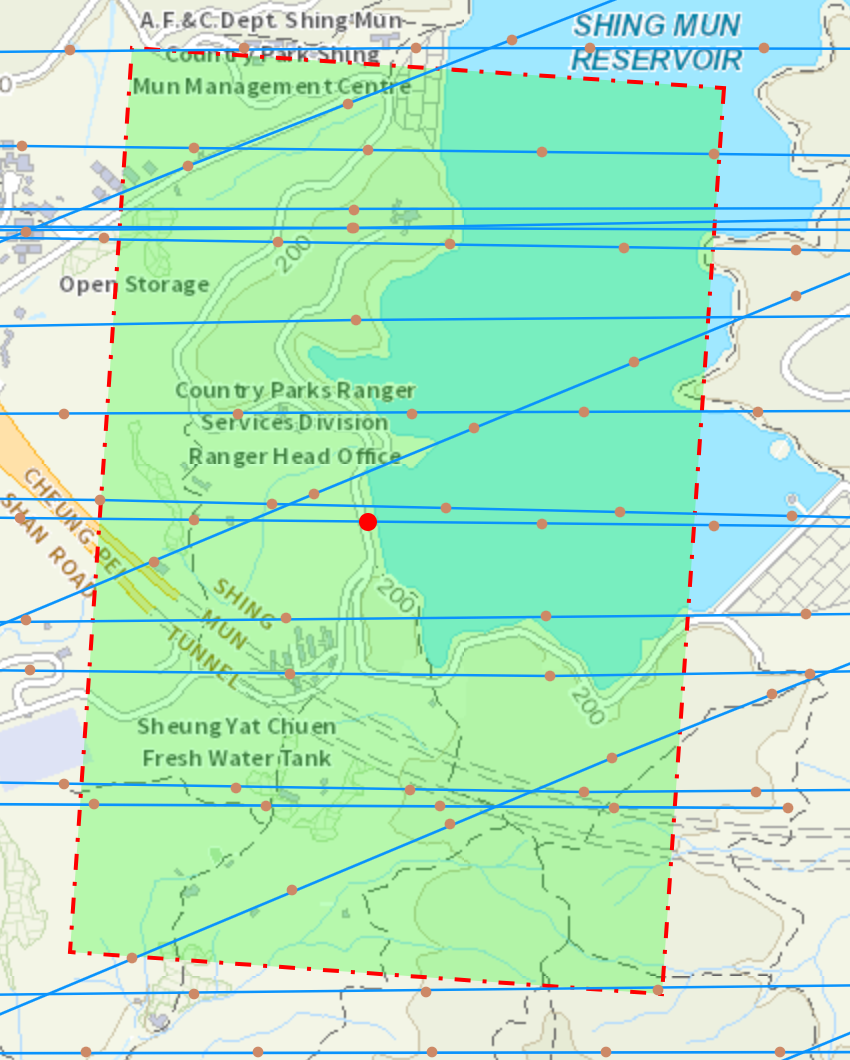
\includegraphics[width=\textwidth]{Included_Images/LandsDept_boundaryLLH.png}
        \caption{Geo-referenced Image Boundary Provided by Lands Department}
    \end{subfigure}
    \hfill
    \begin{subfigure}{0.49\textwidth}
        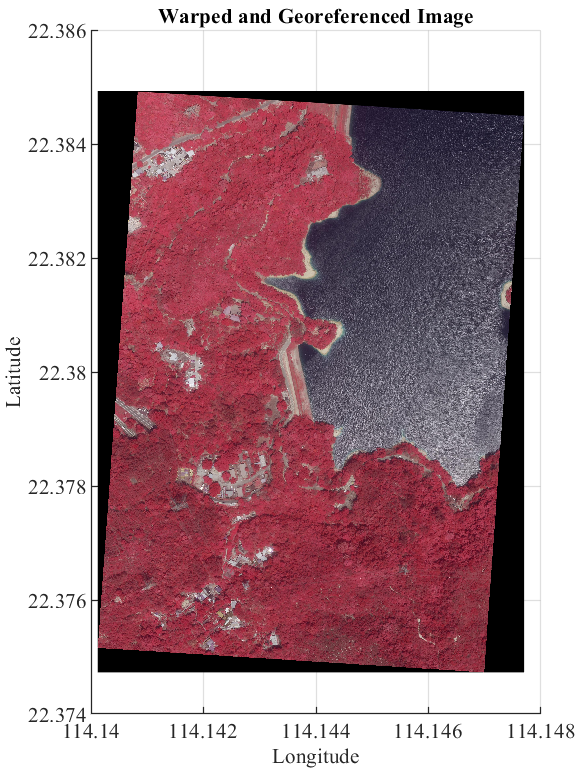
\includegraphics[width=\textwidth]{Included_Images/georeferenced_CIR.png}
        \caption{Transformed and Geo-referenced CIR Image}
    \end{subfigure}
    \caption{Geo-referencing CIR imagery according to the provided image corner coordinates.}
    \label{CIR Georeference}
\end{figure}

Using the longitude and latitude associated with each pixel of the CIR imager,
the red, green, and blue (RGB) channel values of each pixel that lies within a
FFZ could be extracted. The Pearson correlation coefficients between the
RGB values and the GNSS measurement parameters are then calculated to
quantitatively model the correlations between the GNSS measurement parameters
and the CIR image's RGB values within the FFZs: 

\begin{equation}
    r = \frac{\sum (x_i - \bar{x})(y_i - \bar{y})}{\sqrt{\sum (x_i - \bar{x})^2 \sum (y_i - \bar{y})^2}}
\end{equation}

Ultimately, the modelled correlations could be used in reconstructing the colors
represented in the original CIR image from GNSS measurement parameters, such
that the reconstructed CIR image could also inform various ground conditions.

\subsection{Results and Discussion}
In this section, the correlations between GNSS signal parameters and ground
features are qualitatively analyzed and quantitatively modelled from real
experiment data. Ultimately, the potential of the GNSS-R system developed in
this project for vegetation monitoring is demonstrated and discussed for further
improvements. 

\subsubsection{Correlating \texorpdfstring{$C/N_0$}{C/N0} Ratio with Ground
Features} 
After calculating the $C/N_0$ of both the direct and the reflected
signals received onboard the UAV, the ratio of $\frac{C/N_{0, reflected
signal}}{C/N_{0,direct signal}}$ is analyzed with respect to the FFZs of the
reflected signal. This parameter of $C/N_0$ ratio describes the level of
attenuation that the reflected signal experiences. Figure \ref{CNR Ratio FFZ}
below shows the FFZs accumulated over an entire monitoring mission plotted over
a satellite imagery base map, where the colors indicate the $C/N_0$ ratio
between the reflected signal and the direct signal. In areas where multiple FFZs
overlap, the color represents the mean $C/N_0$ ratio of all contributing
signals.

\begin{figure}[H]
    \centering
    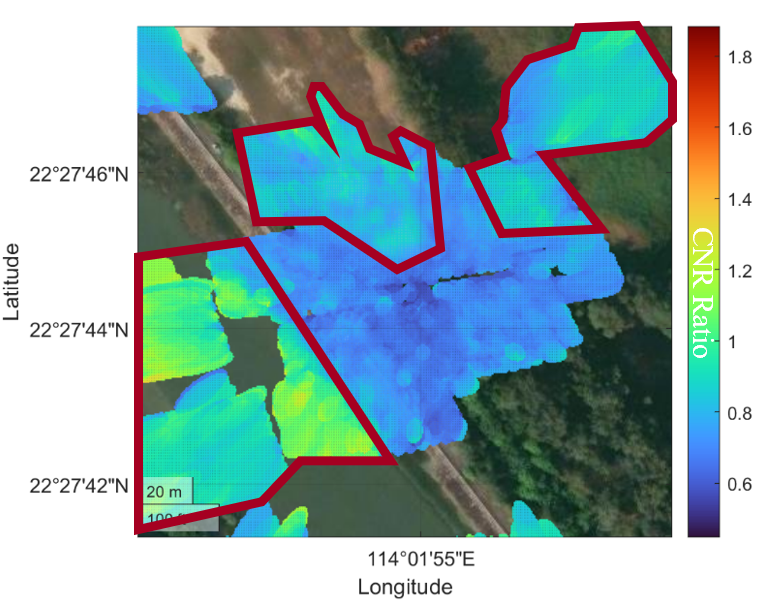
\includegraphics[width=0.8\textwidth]{Included_Images/CNR_ratio_FFZ.png}
    \caption{$C/N_0$ ratio of all signals received during a mission, plotted over the FFZs of the reflected signals.}
    \label{CNR Ratio FFZ}
\end{figure}

From the above, it is evident that when the FFZ is over water or bare soil, the
$C/N_0$ ratio between the reflected and direct signals tends to be higher. This
indicates that stronger reflections occur over water and bare soil compared to
vegetated areas. More importantly, Figure \ref{CNR Ratio FFZ} demonstrates the
capability of $C/N_0$ ratio to clearly outline the boundary between water
surfaces and vegetation canopy. 

Following the qualitative analysis and discussion, the Pearson correlation
coefficient between $C/N_0$ ratio and the RGB values of the CIR image pixels
within each FFZ is calculated. Among all experiments conducted, a consistent
inverse correlation between $C/N_0$ ratio and CIR redness values could be
observed, with the largest absolute value of the correlation coefficient being
over $0.25$ (Figure \ref{CNR_corr}).
\begin{figure}[H]
    \centering
    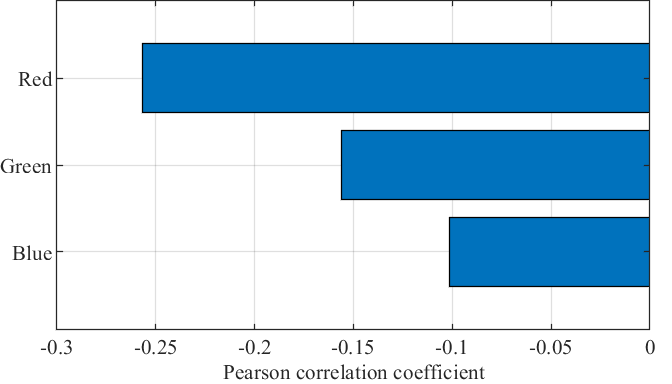
\includegraphics[width=0.8\textwidth]{Included_Images/CNR_ratio_corr_coeff.png}
    \caption{Pearson correlation coefficient between $C/N_0$ ratio and the RGB values of CIR image pixels that fall within the FFZs.}
    \label{CNR_corr}
\end{figure}

\subsubsection{Correlating Excess Pseudorange Delay with Ground Features}
The excess pseudorange delay is also analyzed with respect to the FFZs of the
reflected signal. It represents the additional, unmodelled signal delays of the
reflected signal after the delay due to geometric reflection is effectively
removed. This parameter of excess pseudorange delay primarily describes the
interactions between the reflected GNSS signal and the ground features during
its propagation. Figure \ref{Excess Pr Delay FFZ} below shows the FFZs
accumulated over the entire mission for three of the key experiments conducted
in this project. The colors indicate the excess pseudorange delay of the
reflected signals, and the mean of all contributing signals are taken in areas
where multiple FFZs overlap.

\begin{figure}[H]
    \centering
    \begin{subfigure}{0.8\textwidth}
        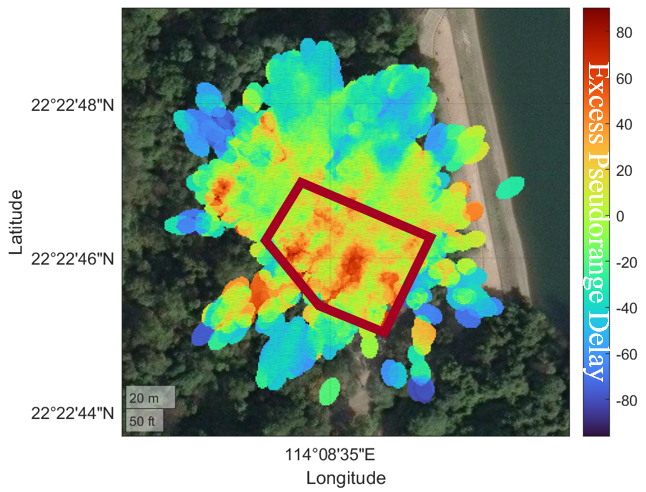
\includegraphics[width=\textwidth]{Included_Images/shingmun_pr_delay.png}
        \caption{Experiment Highlighting Bare Ground Region}
    \end{subfigure}
    \vfill
    \begin{subfigure}{0.8\textwidth}
        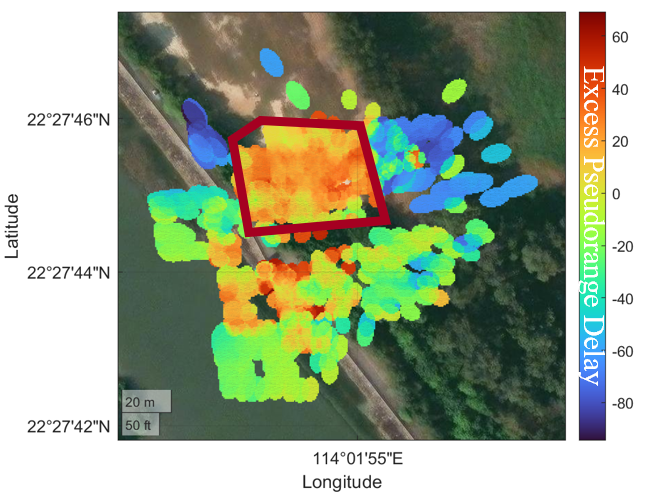
\includegraphics[width=\textwidth]{Included_Images/yuenlong_pr_delay.png}
        \caption{Experiment Highlighting Bare Soil Region}
    \end{subfigure}
    \phantomcaption
\end{figure}

\begin{figure}[H]
    \ContinuedFloat
    \centering
    \begin{subfigure}{0.8\textwidth}
        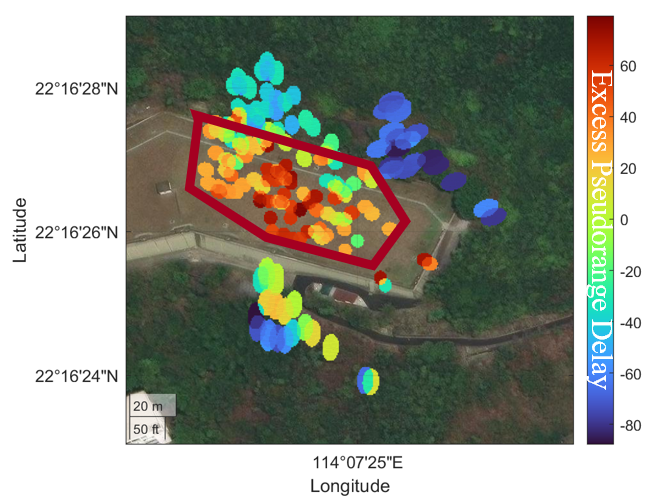
\includegraphics[width=\textwidth]{Included_Images/mtdavis_pr_delay.png}
        \caption{Experiment Highlighting Sparse Vegetation Region}
    \end{subfigure}
    \caption{Excess pseudorange delay of all reflected signals received during three different experiments, plotted over the FFZs of the reflected signals.}
    \label{Excess Pr Delay FFZ}
\end{figure}

The above results indicate that greater excess pseudorange delay could be
observed when the GNSS signals are reflected over bare ground, bare soil, or
sparse vegetation (grassy ground). Notably, the excess pseudorange delay over
dense vegetation tends to be negative, suggesting that the calculation removes
more geometrical reflection delay from the pseudorange than necessary.
Conversely, this implies that the propagation path of the reflected signal is
shorter than the originally expected path, in which the signal propagates
through the vegetation and reflects off the ground (Figure \ref{Reflected Signal
Propagation Path}). Therefore, it is logical to conclude that GNSS signals tend
to reflect off dense tree canopy instead of propagating through them.
Additionally, this negative excess pseudorange delay could potentially serve as
a key input for estimating the vegetation height, as the shortened signal path
is geometrically related to the height of the tree canopy above ground.

\begin{figure}[H]
    \centering
    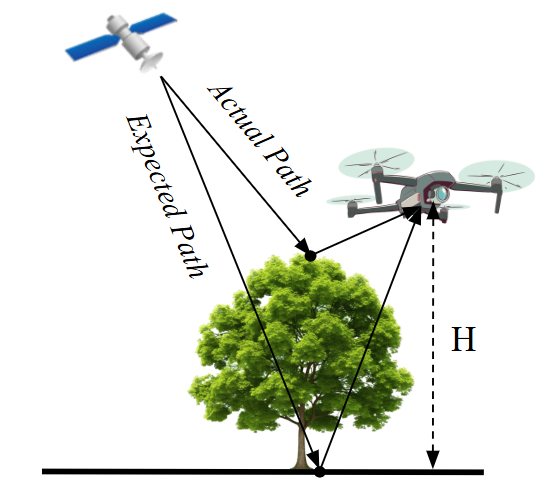
\includegraphics[width=0.55\textwidth]{Included_Images/expected_vs_actual_reflection_path.png}
    \caption{Expected propagation path vs the actual propagation path of the reflected signal.}
    \label{Reflected Signal Propagation Path}
\end{figure}

To quantify the observed correlations between ground features and the GNSS
signal parameters, the Pearson correlation coefficient between excess
pseudorange delay and the RGB values of the CIR image pixels within each FFZ is
calculated. Among all experiments conducted, a consistent positive correlation
between the excess pseudorange delay and CIR greenness and blueness could be
observed, where both correlation coefficients are greater than 0.6 (Figure
\ref{excess_pr_delay_corr}).

\begin{figure}[H]
    \centering
    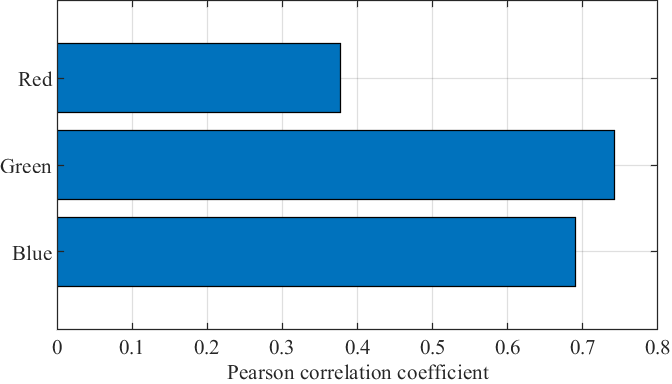
\includegraphics[width=0.8\textwidth]{Included_Images/excess_pr_delay_corr_coeff.png}
    \caption{Pearson correlation coefficient between excess pseudorange delay and the RGB values of CIR image pixels that fall within the FFZs.}
    \label{excess_pr_delay_corr}
\end{figure}

\subsubsection{CIR Imagery Reconstruction}
Through quantitatively modelling the correlations between GNSS measurement
parameters and ground features, a correlation could be found for all three RGB
color channels of the reference CIR image. Therefore, the analysis results
enabled the possibility of reconstructing the colors represented in the original
CIR image from GNSS measurement parameters. An example of the reconstructed CIR
image color over FFZs is shown in Figure \ref{Example Reconstructed CIR} below.
Here, the R values are the inverse of $C/N_0$ ratios, normalized between 0 and
1, while both the G and B values are $0.5$ times the excess pseudorange delay,
normalized between 0 and 1. ($0.5$ is chosen as an arbitrary weighting factor.)
As a result, it is evident that both the water surface and the bare soil areas
could be highlighted through the reconstructed CIR color map over FFZs, which
further demonstrates the potential of GNSS as an alternative remote sensing
system.

\begin{figure}[H]
    \centering
    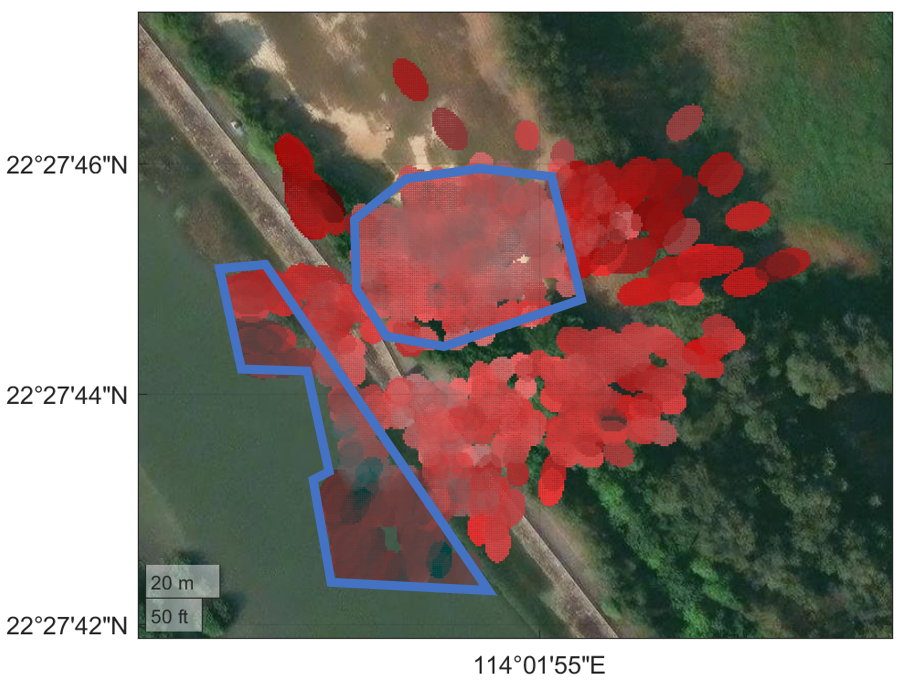
\includegraphics[width=0.8\textwidth]{Included_Images/CIR_reconstruction_yuenlong.png}
    \caption{Reconstructed CIR image color using GNSS measurements, plotted over the FFZs of the reflected signals.}
    \label{Example Reconstructed CIR}
\end{figure}

However, it is also clear that the current approach introduces many noisy
measurements into the sensing system, which may further obscure ground features
that could be retrieved using the GNSS-R system otherwise, such as vegetation
density and height. To investigate the cause of such noisy measurements, the
following experiment was designed and executed. 

\begin{figure}[H]
    \centering
    \begin{subfigure}{0.49\textwidth}
        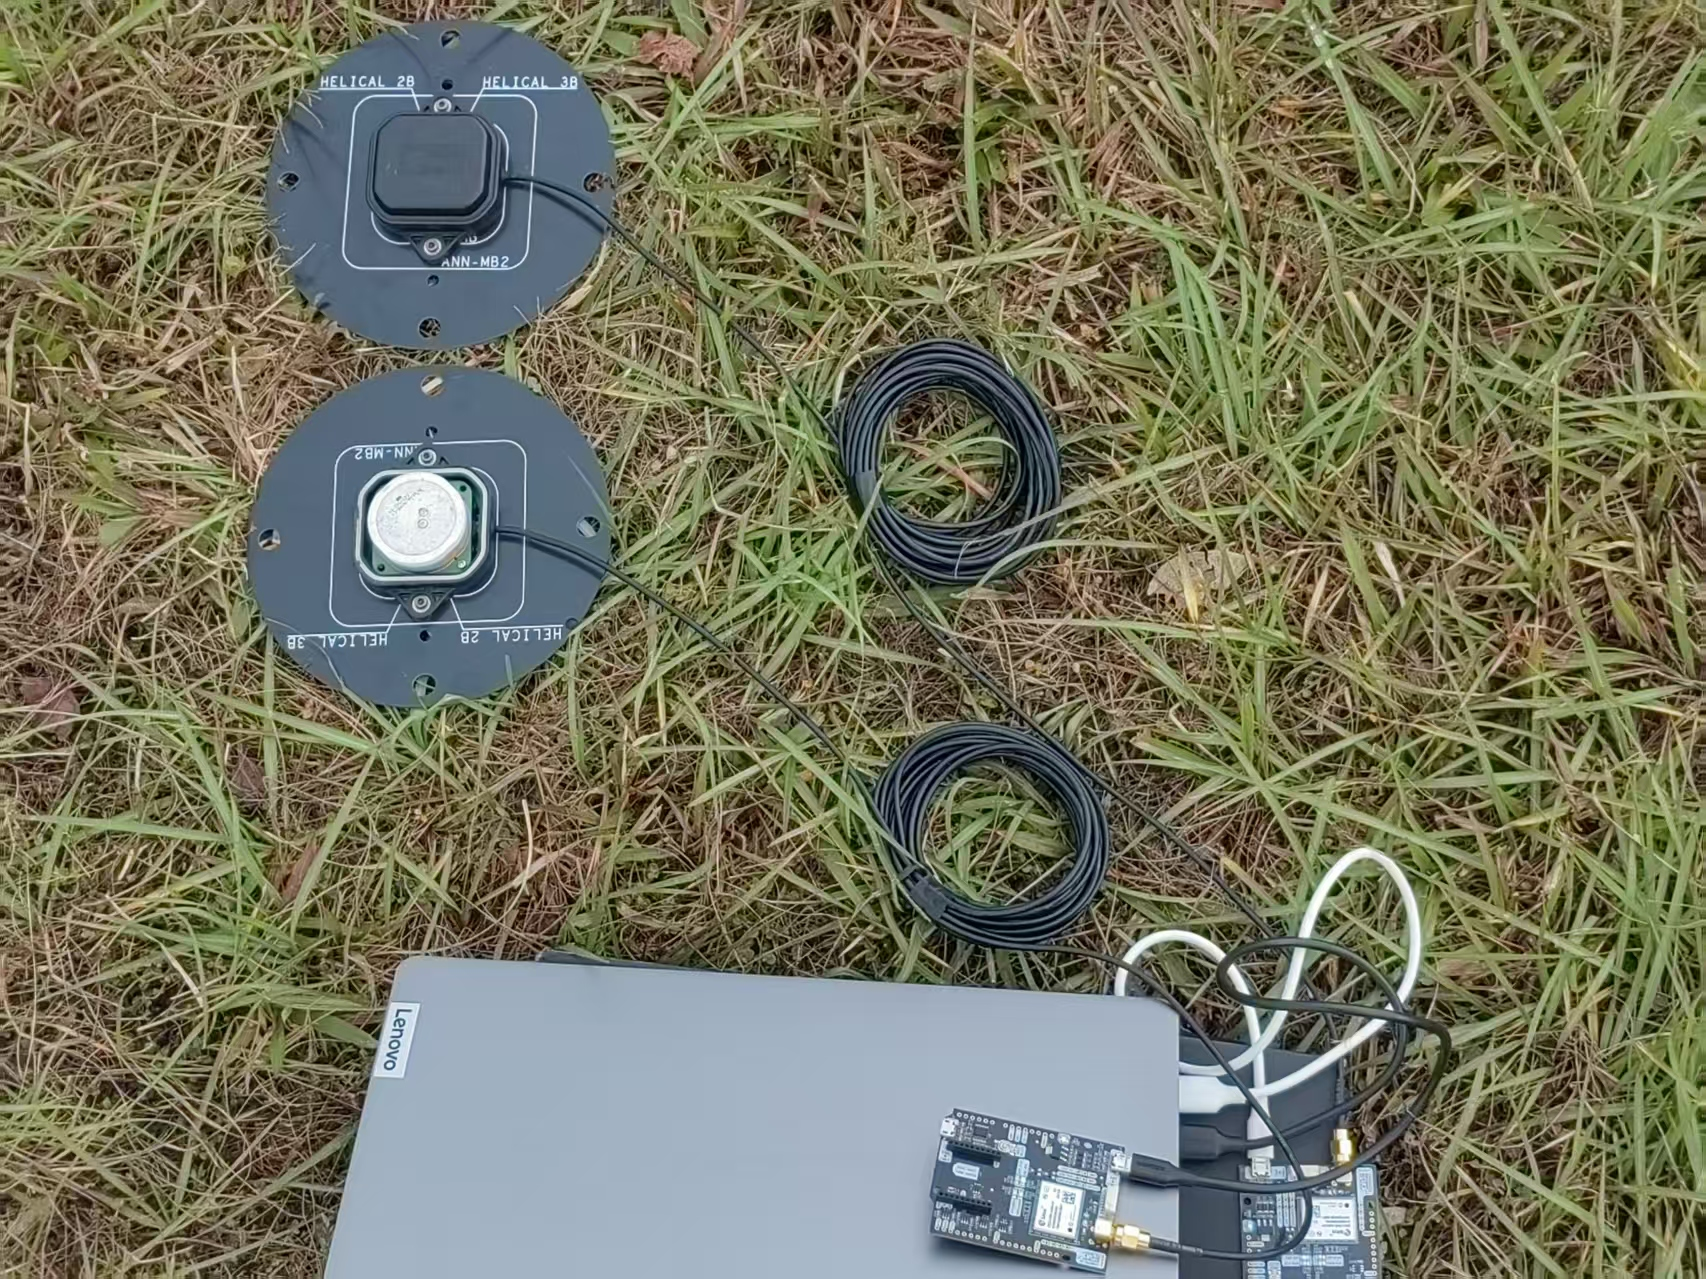
\includegraphics[width=\textwidth]{Included_Images/Open_Sky_Setup.jpg}
        \caption{Experiment Set Up}
    \end{subfigure}
    \hfill
    \begin{subfigure}{0.49\textwidth}
        \centering
        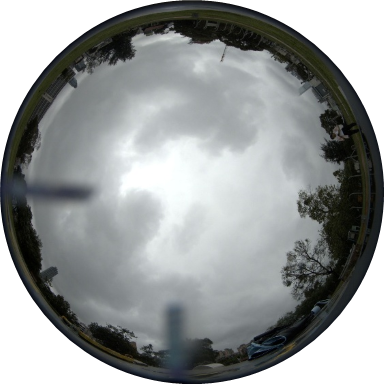
\includegraphics[width=0.75\textwidth]{Included_Images/Open_Sky_Fisheye.png}
        \caption{Fisheye View of the Experiment Environment}
    \end{subfigure}
    \caption{Antenna testing experiment in open sky environment.}
\end{figure}

First, both the zenith RHCP antenna and the nadir LHCP antenna were detached
from the UAV and brought under an open sky environment for testing. Since all
directly transmitted GNSS signals are right-hand circular polarized, it could be
assumed that all signals received under this open sky environment are RHCP
signals. However, in post-processing, the distribution of $C/N_0$ of all signals
received during the experiment reveals the reception of RHCP signals by the LHCP
antenna, just at lower $C/N_0$ values compared to the RHCP antenna due to lower
antenna gains (Figure \ref{CNR_distribution_test}). Therefore, it is possible
that the nadir LHCP antenna received direct signals during the flight missions,
which introduced measurement noises to the dual-antenna system's data and thus
undermined the accuracy and clarity of the reconstructed CIR color map.

\begin{figure}[H]
    \centering
    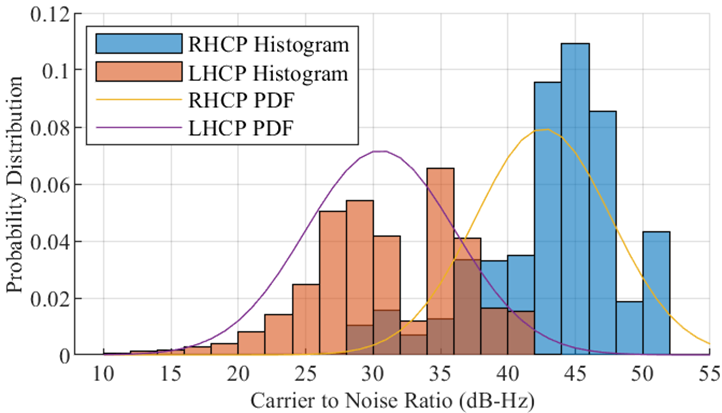
\includegraphics[width=0.75\textwidth]{Included_Images/CNR_Distribution.png}
    \caption{Normalized $C/N_0$ distributions of both antennas.}
    \label{CNR_distribution_test}
\end{figure}

This phenomenon is further demonstrated in a subsequent experiment, where both
antennas were elevated midair. During the first five minutes, both antennas
faced upward; during the final five minutes, both antennas faced downward. The
corresponding $C/N_0$ values received are plotted against observation time in
the figure below.

\begin{figure}[H]
    \centering
    \begin{subfigure}{\textwidth}
        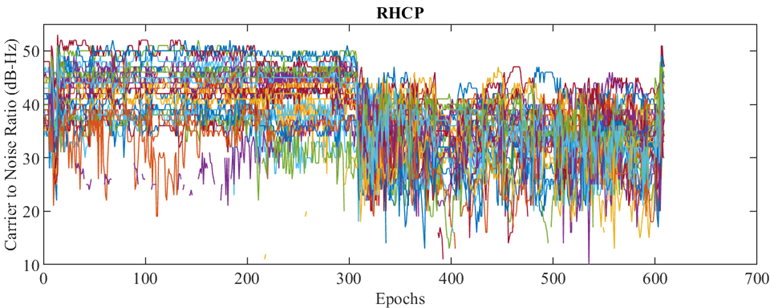
\includegraphics[width=\textwidth]{Included_Images/RHCP_CNR.png}
        \caption{RHCP Antenna}
    \end{subfigure}
    \vfill
    \begin{subfigure}{\textwidth}
        \centering
        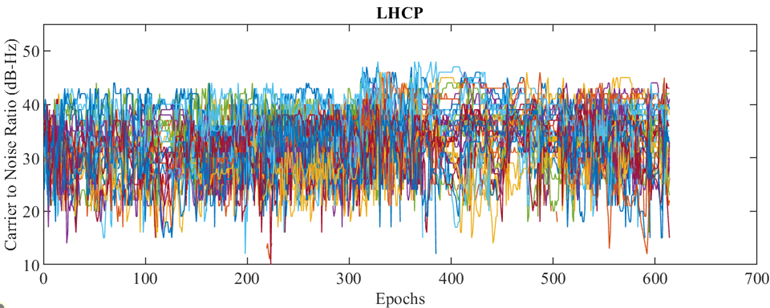
\includegraphics[width=\textwidth]{Included_Images/LHCP_CNR.png}
        \caption{LHCP Antenna}
    \end{subfigure}
    \caption{$C/N_0$ values received by both antennas during the experiment.}
\end{figure}

The above observations are then qualitatively summarized in the table below:

\begin{table}[H]
    \centering
    \caption{Summary of $C/N_0$ behaviors for both antennas under different
    signal reception scenarios.}
    \begin{tabular}{|c|c|c|}
    \hline
     & \textbf{Direct Signal} & \textbf{Reflected Signal} \\
    \hline
    \textbf{RHCP Antenna} & High $C/N_0$ & Low $C/N_0$ \\
    \hline
    \textbf{LHCP Antenna} & Low $C/N_0$ & High $C/N_0$ \\
    \hline
    \end{tabular}
\end{table}

Since both direct and reflected signals can be received by both the zenith RHCP
antenna and the nadir LHCP antenna, and their signal properties differ based on
signal polarization, it is critical to classify all received signals to
distinguish reflected signals from direct signals in a robust GNSS-R system. One
possible method is to leverage the differences in $C/N_0$ values observed by
different antenna polarizations and create a decision threshold to separate
direct and reflected signals. However, as illustrated in Figure
\ref{CNR_distribution_test}, the distribution of $C/N_0$ values of both antennas
overlap each other, making it difficult to obtain a clear decision boundary.
Therefore, multiple parameters may be necessary to conduct such classification
tasks, such that machine learning approaches may offer a much more effective
solution. The classification of signals and the detection of vegetation area
boundaries using machine learning models is detailed in the section below, where
the results in the machine learning pipeline will ultimately be used to
cross-validate the results from the GNSS-R pipeline, which is demonstrated in
the case study.


% --- Machine Learning ---
\section{Machine Learning}

\subsection{Literature Review}
A part of this project will be to develop a deep learning based model that can
process collected GNSS-R data and address two main topics: (1) Classification of
the received signals into direct and reflected signals, and (2) Prediction of
vegetation parameters from the raw GNSS data. The goal will be to develop and
test tree based and neural network based models that take GNSS-R features, both
publicly available and collected by our UAV system, as inputs and output the
desired results. The model training will be optimized for highest computational
efficiency and accuracy on python based PyTorch framework. Past research has
demonstrated that GNSS-R can sense vegetation as the reflected signal power and
modulation depends on vegetation cover and moisture. For example, a study by
Small et al. (2010) and others found that the amplitude of the reflected GNSS
signal to Noise Ratio (SNR) oscillations over crops correlated linearly with
Vegetation Water Content (VWC) \cite{small2010sensing}. A study by Chen et al.
(2024) recently derived a new GNSS-R vegetation index and used Artificial Neural
Networks (ANN) to retrieve VWX from spaceborne data, achieve a correlation of
approximately 0.94 with reference measurements \cite{chen2024new}. Other studies
have trained deep learning models on GNSS-R features. One study trained an ANN on
Delay Doppler Maps (DDMs), SNR, signal incidence angle and geographic data to
predict the Above Ground Biomass (AGB) \cite{pilikos2024biomass}. Prior GNSS-R
vegetation retrieval efforts have focused on parameters like biomass, soil
moisture, and VWC. For example. SNR that has been reflected from wheat was used
to estimate the height and water content of wheat, which signifies that strong
vegetation attenuates the reflected signals \cite{zhang2017use}. Polarimetric
GNSS features have also been used in previous studies. Cross polarization ratios
and co polarized reflection coefficients were found to be sensitive to
vegetation biomass and moisture \cite{wu2021recent}. 

Most existing studies have used spaceborne or terrestrial platforms, while UAV
based GNSS-R remains underexplored. The few existing UAV based works demonstrate
feasibility but do not address vegetation mapping
\cite{wu2021recent,chen2024new}. Moreover, classification of difference signals
is not a well studied topic. However, existing study suggests that GNSS-R
features can inform vegetation parameters \cite{small2010sensing}. But the gap
is clear: GNSS-R with UAVs for vegetation mapping and signal classification has
not been demonstrated. This project will bridge the gap by developing ML models
tailored for UAV scale GNSS-R data and the specific tasks of vegetation
detection and parameters estimation. 

\subsection{Methodology}
The projects aim to utilize machine learning algorithms for two purposes:
(1) to classify the received signals into three classes: reflected from ground,
direct to down antenna and reflected from trees, and (2) to predict vegetation 
properties based on the features extracted from GNSS measurements.
\begin{figure}[H]
    \centering
    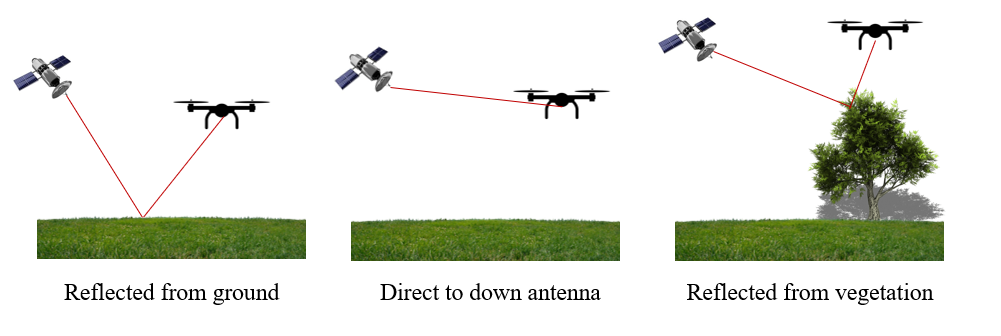
\includegraphics[width=1\textwidth]{Included_Images/Classes.png}
    \caption{Classes of signals to be classified.}
\end{figure}
So far, only the first part has been attempted. A supervised learning approach was taken, where a dataset was
constructed from collected GNSS data with labels assigned based on the collection scenarios.
The collected data was analyzed and features were then selected to train a classification model. 
The details of the feature analysis, dataset construction, feature selection and model training 
are outlined in the following sections.

\subsubsection{Feature Analysis}
Before constructing and training a classification model, the collected GNSS 
measurements were analyzed to identify potential features that could help
distinguish between reflected and direct signals. Four major features were
found to have different distributions between the two scenarios, which are UAV hovering 
over trees and UAV hovering over bare ground. These features are outlined below:

\paragraph{Carrier to Noise Ratio (C/N0)} ~\\
From the figures below, It can be observed that the $C/N_0$ values for signals
reflected from trees are generally lower than those for signals getting
reflected from the bare ground. This indicated that vegetation attenuated the
GNSS signal quality. The figures also illustrate a wider spread of $C/N_0$
values for signals reflected from trees compared to those from bare ground, in
which case the signal distribution is more concentrated. 
\begin{figure}[H]
    \centering
    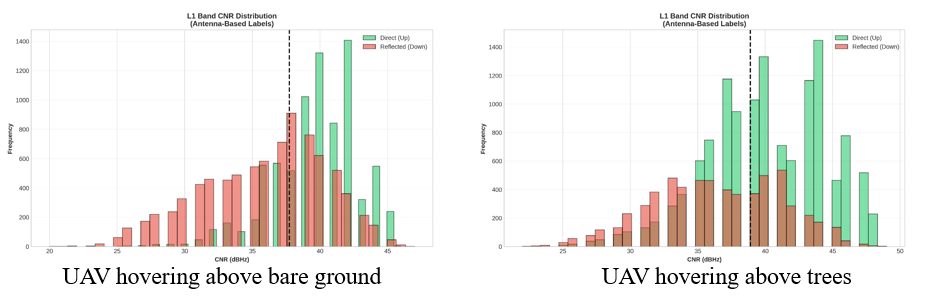
\includegraphics[width= 1\textwidth]{Included_Images/CNR.png}
    \caption{Distribution of $C/N_0$ for signals reflected from trees and bare ground.}
\end{figure}
    
\paragraph{Pseudorange} ~\\
Similar to $C/N_0$, the pseudorange values for signals
reflected from trees display an increased pseudorange bias and variance, which produces a
clear decision boundary for the classifier than that of bare ground signals.
Some of the pseudorange values for signals reflected from trees are extremely high, which 
might be due to the multipath effect caused by dense vegetation. The figures below
illustrate the distribution of pseudorange values for signals reflected from trees
and bare ground.
\begin{figure}[H]
    \centering
    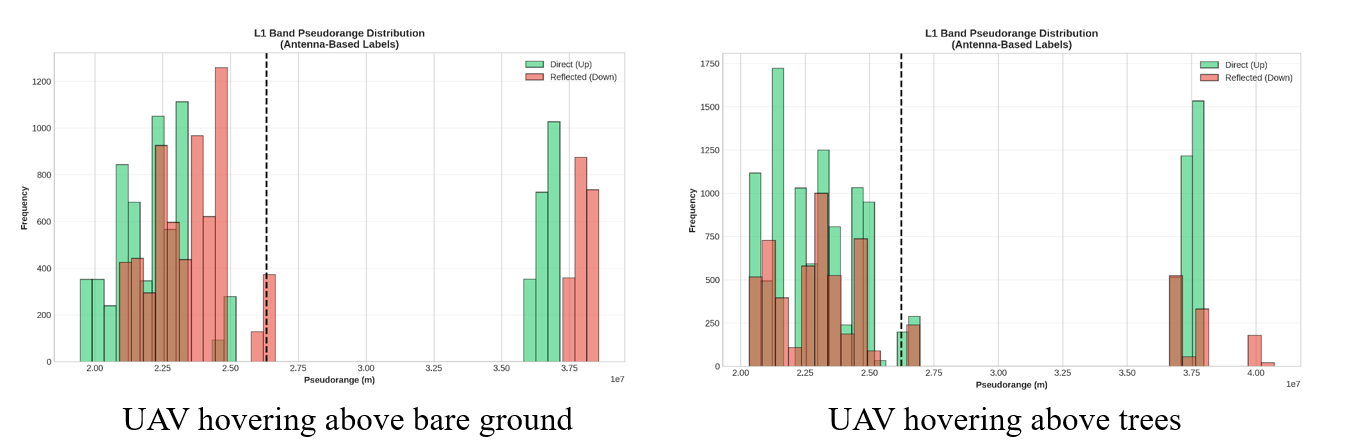
\includegraphics[width= 1\textwidth]{Included_Images/Pseudorange.png}
    \caption{Distribution of pseudorange for signals reflected from trees and bare ground.}
\end{figure}
    
\paragraph{Doppler measurement} ~\\
Doppler measurement refers to the instantaneous shift in frequency of the
received GNSS carrier signal due to the relative velocity between the satellite
and the receiver. As can be seen from the figures below, the Doppler values for
signal reflected from trees are clearly distinguishable from those reflected
from bare ground. For the case of bare ground, the Doppler values for up and
down antenna are almost identical. However, for the case of UAV hovering over
vegetation, the Doppler distribution is more spread out, ranging from
approximately -5000 dB-Hz to 4000 dB-Hz. This indicates that reflections caused
by trees introduce additional frequency shifts in the received signals. The
figure below illustrates the distribution of Doppler values for signals
reflected from trees and bare ground.
\begin{figure}[H]
    \centering
    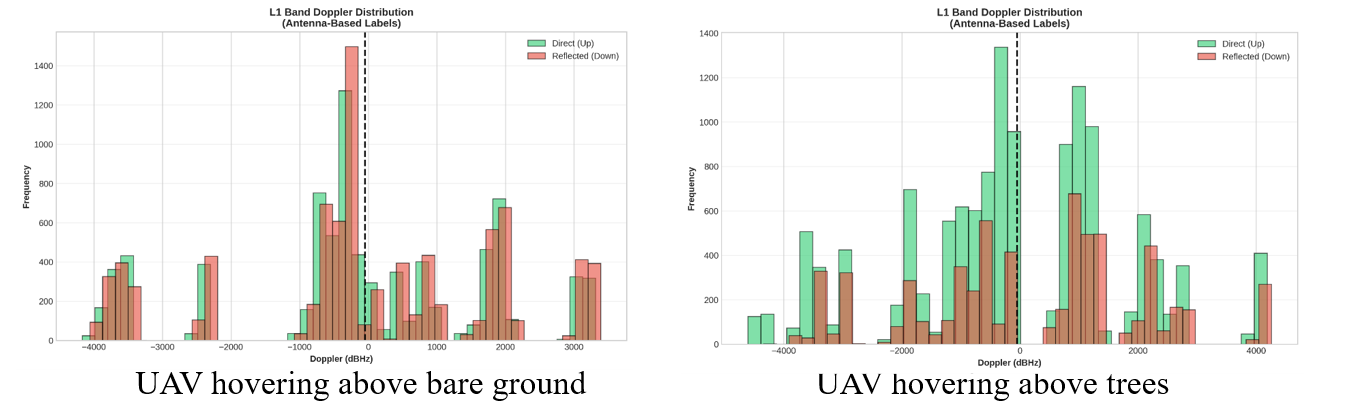
\includegraphics[width= 1\textwidth]{Included_Images/doppler.png}
    \caption{Distribution of Doppler for signals reflected from trees and bare ground.}
\end{figure}
    
\paragraph{Carrier Phase} ~\\
Carrier phase refers to the precise range observables that are derived from the
accumulated phase cycles of the GNSS carrier wave. From the figure below, it can
be observed that the carrier phase values for signals reflected from trees
exhibit 2.5 times broader carrier phase spread compared to those reflected from
bare ground, reflecting multipath induced phase delays versus the concentrated
phase coherence of bare ground reflections. This indicated that vegetation
introduces additional phase shifts in the received signals. The figure below
illustrates the distribution of carrier phase values for signals reflected from
trees and bare ground.
\begin{figure}[H]
    \centering
    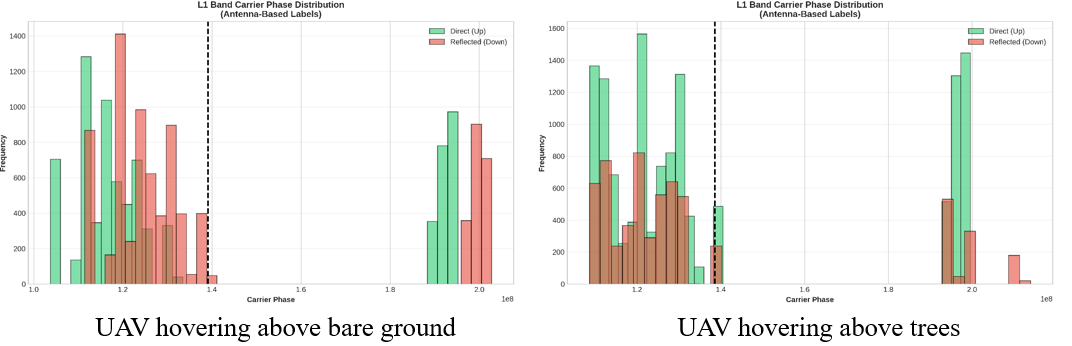
\includegraphics[width= 1\textwidth]{Included_Images/Carrier Phase.png}
    \caption{Distribution of carrier phase for signals reflected from trees and bare ground.}
\end{figure}


\subsubsection{Dataset Construction}
To train a robust model that can classify different signal types, constructing a clean 
and reliable dataset was one of the most important aspect of this pipeline. In order to 
do so, data was collected across multiple real world conditions with distinct environmental
features. The goal was to ensure the dataset captures the full diversity of GNSS-R signal 
behavior encountered during different UAV operations. Three collected scenarios were defined which 
are listed below:
\begin{enumerate}
    \item \textbf{Open Sky}: The receiver was held in an unobstructed environment with a clear
    Line-of-Sight (LOS) to the GNSS satellites. This was done to produce predominantly direct LOS signals.
    \item \textbf{UAV hovering over bare ground}: Signals captured in this scenario are dominated by specular 
    reflections from the ground surface. This is a representative of non vegetated terrain or ground reflected
    signals. 
    \item\textbf{UAV hovering over trees}: This scenario introduces diffuse reflections caused by vegetations. 
    This dataset can represent the qualitative change in signal characteristics due to scattering from vegetation which 
    is different from that of bare ground reflected ones.
\end{enumerate}
\begin{figure}[H]
    \centering
    \begin{subfigure}{0.33\textwidth}
        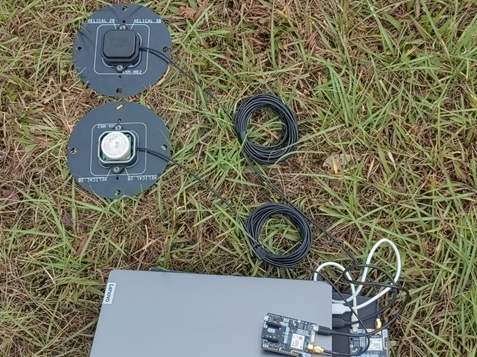
\includegraphics[width=\textwidth]{Included_Images/opensky.png}
        \caption{Open Sky}
    \end{subfigure}
    \hfill
    \begin{subfigure}{0.3\textwidth}
        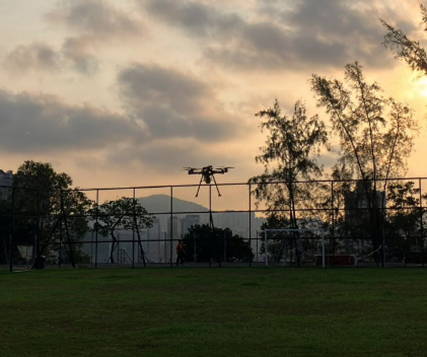
\includegraphics[width=\textwidth]{Included_Images/bareground.png}
        \caption{UAV hovering over ground}
    \end{subfigure}
    \hfill
    \begin{subfigure}{0.29\textwidth}
        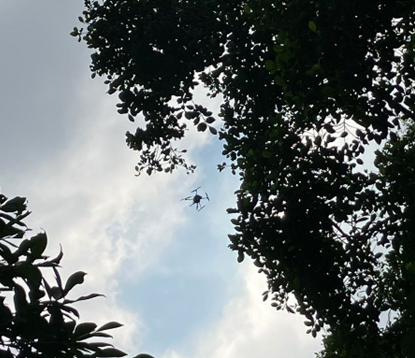
\includegraphics[width=\textwidth]{Included_Images/overtrees.png}
        \caption{UAV hovering over trees}
    \end{subfigure}
    \caption{Data collection scenarios.}
\end{figure}

Each scenario corresponds directly to one of the three target classes used in classification.
Labelling was then done based on the known collection scenarios. Open sky data were assigned as 
direct signals class, bare ground samples were assigned as ground reflected signals class and lastly the 
data collected by hovering the UAV over trees were assigned as tree reflected signals class. This scenario based
labelling strategy relies on the assumption that the dominant signal type in 
each environment is consisted with the respective controlled environments. However, noise is inevitable in the collected datasets,
for example, direct signals may occasionally be captured during ground hovering flights. Nonetheless, the approach is pragmatic and aligns with 
the practical constraints of field data collection in real world. 

The collected data comprised of 70,125 labelled samples drawn from all three scenarios. To address potential class 
imbalance that could bias the model toward more frequently occurring signal types a balanced class weight strategy was applied during training. This effectively
upweights minority classes in the loss function. Overall, this multienvironment data collection strategy ensures 
that the model generalizes well across all three classes. This is a critical for deployment on a UAV operative across different terrain conditions.


\subsubsection{Model Selection}
For the classification task, a LightGBM model was selected due to its advantages
with native support for NaN values. This feature of the model is particularly
important for our case as raw GNSS data often contains missing values due to
signal blockages or receiver limitations. Cleaning the data by removing the NaN
values would lead to significant loss of data, as cleaning process would have to
be carried out either row-wise or column-wise. Replacing the NaN values with
zeros or mean values would introduce bias to the dataset, which would
potentially affect the performance of the model. Therefore, using a model with
native support for NaN values was the most suitable approach for our case. Below
is a brief introduction to LightGBM model. \paragraph{LightGBM Model} ~\\
LightGBM (Light Gradient Boosting Machine) is a highly efficient framework 
for gradient boosting decision trees (GBDT) that was developed by Microsoft
\cite{ke2017lightgbm}. The model is similar to popular GBDTs such as XGBoost;
however, it addresses some of the limitations of these models in terms of efficiency 
and scalability for large datasets with high-dimensional features \cite{ke2017lightgbm}.

Unlike level wise tree growth that can be seen in traditional GBDT models, 
LightGBM uses a leaf-wise growth strategy as can be seen in the figure below \cite{ke2017lightgbm}. 
\begin{figure}[H]
    \centering
    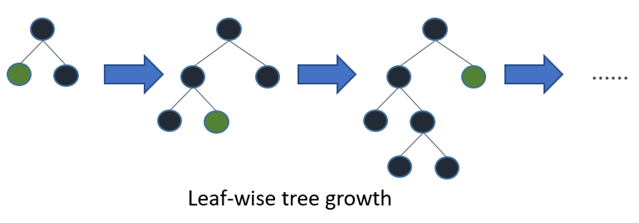
\includegraphics[width=0.9\linewidth]{Included_Images/LightGBM.png}
    \caption{Leaf-wise strategy for tree growth}
\end{figure}
It expands the leaf with the maximum variance gain at each step, as shown in the formula below:
\begin{equation}
V_{j|o}(d) = \frac{1}{n_o} \left( \frac{ \left( \sum_{ {x_i \in O: x_{ij} \leq d} } g_i \right)^2 }{ n_l^o(d) } + \frac{ \left( \sum_{ {x_i \in O: x_{ij} > d} } g_i \right)^2 }{ n_r^o(d) } \right),
\end{equation}
where $V_{j|o}(d)$ is the variance gain, $g_i$ are the gradients, $n_o$ is the number of samples in the parent node. This approach 
optimizes boosting and leads to faster convergence when combined with gradient-based sampling. 

LightGBM also provides native support for NaN values through optimal 
directional assignment during splits. This helps to avoid manual imputation 
of data that could introduce bias. 


\subsubsection{Model Training}
In order to train the LightGBM model, the dataset was first split into training,
testing, and validation sets. The ratio for dataset division was 60:20:20 respectively. A total of 70,125 
labeled samples were used for training the model. The training features included pseudorange, 
Carrier to Noise Ratio, Doppler measurement, Pseudorange Error and Carrier Phase.
The tuning of hyperparameters was then performed using a grid search approach and the used 
hyperparameters are shown in the table below. 
\begin{table}[H]
\centering
\label{tab:lgbm-hyperparams}
\renewcommand{\arraystretch}{1.2} % Increase row height for better readability
\begin{tabular}{ll}
\toprule
\rowcolor{lightgray}
\textbf{Hyperparameter} & \textbf{Value} \\
\midrule
objective & multiclass \\
n\_estimators & 2000 \\
\rowcolor{gray!10}
num\_leaves & 96 \\
learning\_rate & 0.02 \\
\rowcolor{gray!10}
boosting\_type & gbdt \\
max\_depth & -1 \\
\rowcolor{gray!10}
min\_child\_samples & 20 \\
min\_child\_weight & 1e-3 \\
\rowcolor{gray!10}
reg\_alpha & 0.5 \\
reg\_lambda & 1.0 \\
\rowcolor{gray!10}
subsample & 0.8 \\
subsample\_freq & 1 \\
\rowcolor{gray!10}
colsample\_bytree & 0.8 \\
class\_weight & balanced \\
\rowcolor{gray!10}
random\_state & 42 \\
\bottomrule
\end{tabular}
\caption{Hyperparameters for LGBM Classifier}
\end{table}
As can be seen from the table above, a multi-class objective function was used
to classify the signals into three classes. This is because the dataset contains
three classes of signals: direct signals, signals reflected from ground and
signals reflected from trees. The training objective here is the multinomial 
cross entropy loss function. Let $K$ be the number of classes and $N$ be the number of samples.
For each of the samples $i$,  the model output of raw scores $\mathbf{f}_i =
\{f_{i,1}, \dots, f_{i,K}\}$, which are converted into probabilities using the softmax function:
\begin{equation}
    p_{i,k} = \frac{e^{f_{i,k}}}{\sum_{j=1}^{K} e^{f_{i,j}}}
\end{equation}

where $p_{i,k}$ is the predicted probability of sample $i$ belonging to class $k$. 
The overall loss function minimized during training is given by:
\begin{equation}
    \mathcal{L}=
-\frac{1}{N}
\sum_{i=1}^{N}
\sum_{k=1}^{K}
y_{i,k} \log(p_{i,k}),
\end{equation}
where $y_{i,k}$ is a binary indicator that equals 1 if the true class of
sample $i$ is $k$, and 0 if not. LightGBM optimizes this loss using
gradient boosting with second order Taylor approximation, which leverages both
the first (gradient) and second order derivatives (hessian) of the loss with respect to the
model outputs \cite{ke2017lightgbm}. The corresponding gradients and hessians are computed as follows:
\begin{equation}
g_{i,k}
=
\frac{\partial \mathcal{L}}{\partial f_{i,k}}
=
p_{i,k} - y_{i,k},
\end{equation}
\begin{equation}
h_{i,k}
=
\frac{\partial^2 \mathcal{L}}{\partial f_{i,k}^2}
=
p_{i,k}(1 - p_{i,k}).
\end{equation}
These are used to fit decision trees in a leaf wise manner, where at each iteration,
the model adds a new tree that predicts the negative gradients of the loss function \cite{ke2017lightgbm}.
The model converged well and the loss curves for training and validation sets are shown in the figure below.
\begin{figure}[H]
    \centering
    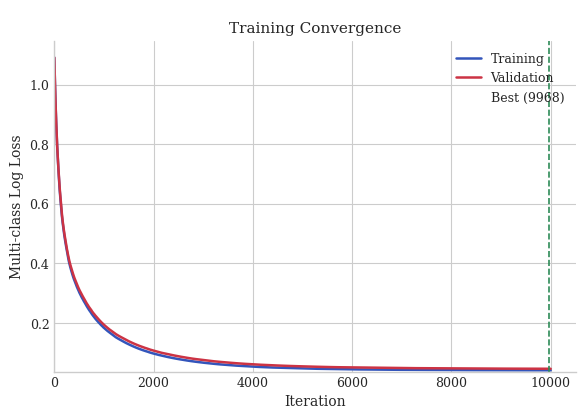
\includegraphics[width=1\linewidth]{Included_Images/LossCurve1.png}
    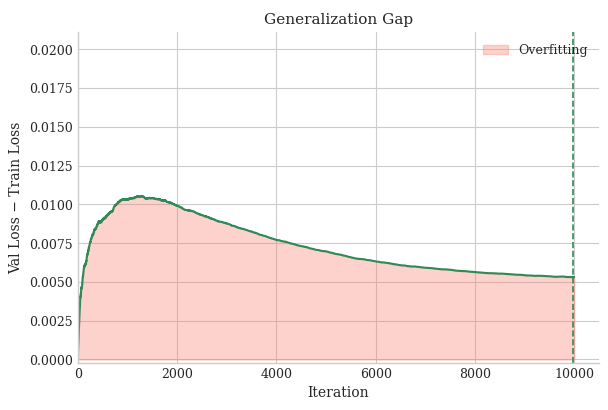
\includegraphics[width=1\linewidth]{Included_Images/LossCurve2.png}
    \caption{Training and Validation Loss Curves for LightGBM.}
\end{figure}



To gain insight into the LightGBM model's training process, two plots were
plotted: a convergence plot of the multi-class log loss as a function over each
iteration for the training and the validation sets, and the generalization plot
that compares the difference between the validation loss and the training loss
for each boosting iteration.

\paragraph{Training Convergence}:
The left plot shows the convergence of the multi class log loss over
100000 boosting iterations for both the training and validation sets. Both the
losses start around a value of 1. This basically indicates uncertainty of the 
model before any training was done. As training starts for the first 1000 boosting rounds
the loss decreases significantly. This is due to the fact that the gradient boosting 
trees make the largest corrections to the model predictions. This is a typical characteristic of 
gradient boosting models. After this, the rate of improvement slows down where each additional 
tree makes smaller adjustments. Around 3000 to 4000 epochs the curves start to plateau and loss stabilizes below a 
value of 0.1. The best iteration was 9968 which is marked with the dashed vertical line. 

\paragraph{Generalization Plot}:
The other plot on the right quantifies the generalization gap. This gap is defined as
the pointwise difference between validation loss and training loss ($\mathcal{L}_{\text{val}} - 
\mathcal{L}_{\text{train}}$) across iterations. The positive gap is expected since the model 
has not seen the validation data during training and only been optimized on the training set. The main 
observation here is whether this gap increases over training epoch or decreases. 

Early in training process the gap rises from near zero to a peak value of 0.01-0.011 around iterations
1500-2000. The initial rise of this value is due to the aggressive fast learning of the model where the model 
is trying to fit the data. However, after this the gap narrows progressively and reaches an approximate value of 0.005-0.006
by 10000 iterations. This is a positive indication as it means the model progressively generalize rather than simply 
memorizing the training data. The shaded region in the plot is the overfitting zone and the magnitude is negligible. This does not 
meaningfully comprise the model's performance on unseen data.

Combined, both the panels affirm that the LightGBM model has converged and generalized well, 
which is a formidable basis of the signal classification task. The additional quantitative testing of the classification 
performance of the model is provided in the Results and Discussion section.

\subsection{Results and Discussion}
As classification of the reflected and direct signals is required for robust GNSS-R
implementation, the LightGBM model is trained to classify the signals based on
the features extracted from both antennas. The data collection, dataset preparation, and model
selection have been explained in the methodology section. The performance evaluation of the model is done
based on various metrics including F1 score, confusion matrix and Receiver Operating Characteristic (ROC) curve. The subsections
below present the evaluation results and discussion.
\subsubsection{F1-score}
The F1 score is the mean of two performance indicators: precision and recall of a classification model. Precision of a model indicates
the ability of a model to not label a negative sample as positive. On the other hand, recall indicates the ability of a model to 
find all the positive samples. The F1-score is calculated using the following equation:
\begin{equation}
    F1 = 2 \cdot \frac{Precision \cdot Recall}{Precision + Recall}
\end{equation}
The F1-score for the LightGBM model on the test dataset is shown in the figure below.
\begin{figure}[H]
    \centering
    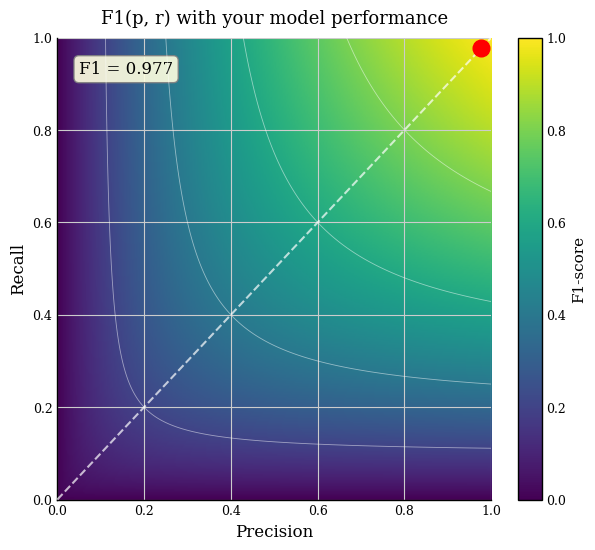
\includegraphics[width=1\textwidth]{Included_Images/F1.png}
    \caption{F1-score for LightGBM model on test dataset}
\end{figure}
From the figure above, it is observed that the LightGBM model achieves an F1 score of approximately
0.977 on the test dataset, where a value of 1 represents a perfect model. This indicates that the model has a proper balance between precision and recall and
is effective in classifying different classes of signals. 
\subsubsection{Confusion matrix}
Confusion matrix can help to visualize the performance of a classification model on a set of test data for which
the true values are already known. The elements which are present diagonally in the matrix 
represent correctly classified samples and the rest of the elements indicate the number of incorrect classified samples. 
The confusion matrix for the LightGBM model is shown below.
\begin{figure}[H]
    \centering
    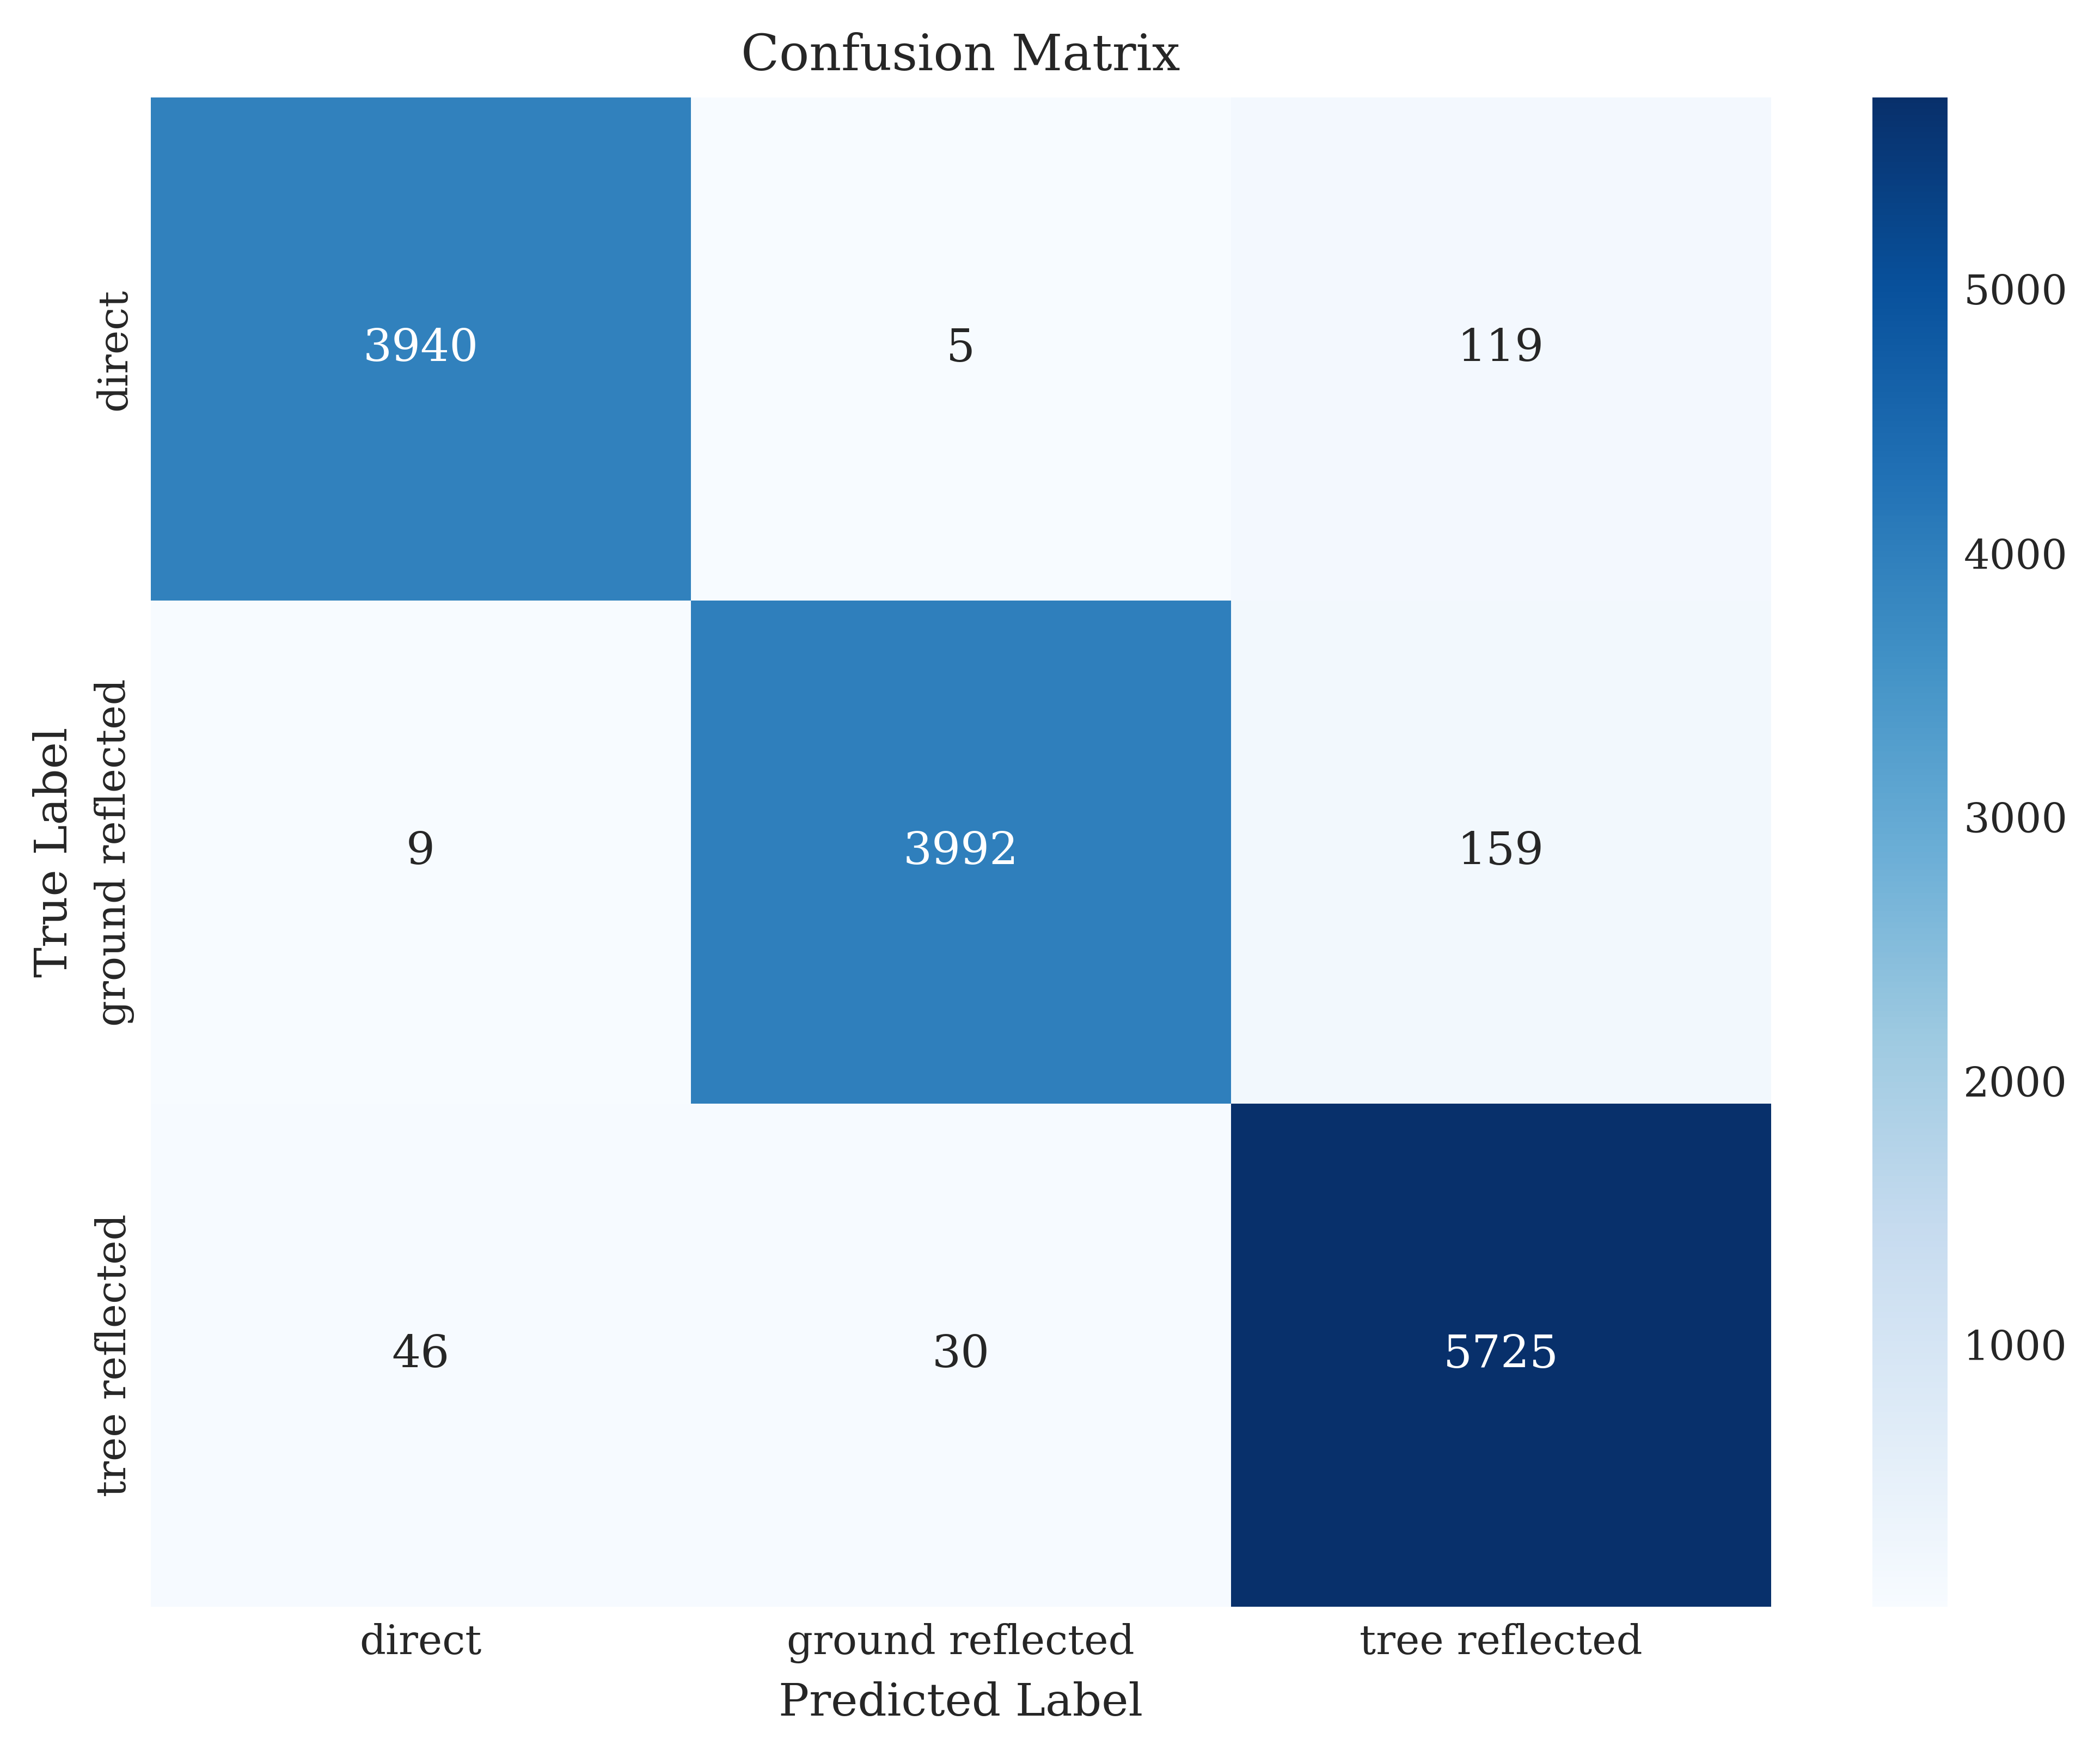
\includegraphics[width=1\textwidth]{Included_Images/Confusion-matrix.png}
    \caption{Confusion matrix for LightGBM model}
\end{figure}
From the confusion matrix above, it is observed that the LightGBM model has correctly classified a majority 
of the samples in the test dataset. Primary confusion for the model occurs for direct and ground reflected signals being classified as 
tree reflection. As can be observed from the confusion matrix, 119 and 139 samples of direct and ground reflected
signals respectively are misclassified as tree reflected signals. This could be due to the similarity in the features of these
signals. However, the model has performed well in classifying tree reflected signals with only 76 samples being misclassified. 
These results are acceptable as the model will later be used primarily to identify vegetation-reflected signals.
\subsubsection{ROC Curve}
A ROC curve is a way to graphically represent how well a binary classifier is performing at different threshold settings. 
It generally plots the True Positive Rate (TPR) against the False Positive
Rate (FPR). This technique helps to visualize the trade-off between sensitivity and specificity of the model. If the ROC value is
closer to 1, it indicates that the model can effectively distinguish between classes, while a value near
0.5 indicates little discrimination ability. For the LightGBM model trained for classification of signals,
the ROC curve is shown in the figure below.
\begin{figure}[H]
    \centering
    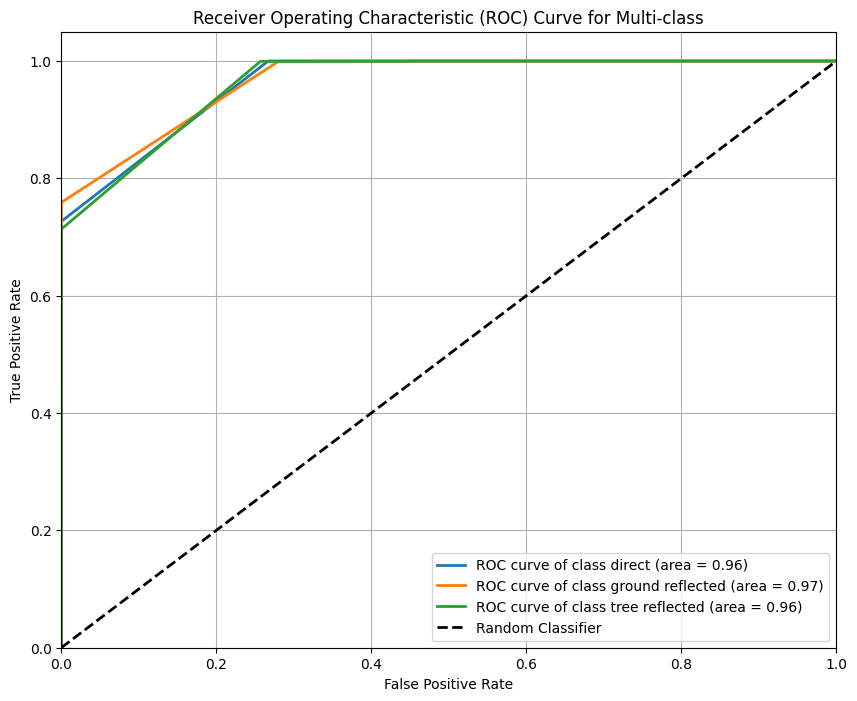
\includegraphics[width=1\textwidth]{Included_Images/ROC.png}
    \caption{ROC curve for LightGBM model on test dataset}
\end{figure}
The figure indicates that the LightGBM model has a ROC value of over 0.95 for all three classes of signals, meaning
that the model has high ability to distinguish between signal classes.
\subsubsection{Feature Importance}
Feature importance is a technique in machine learning used to identify and rank the most relevant features
in a model. A feature importance analysis was performed on the LightGBM model to identify the most crucial features for
 signal classification task. The feature importance plot is shown in the figure below.
\begin{figure}[H]
    \centering
    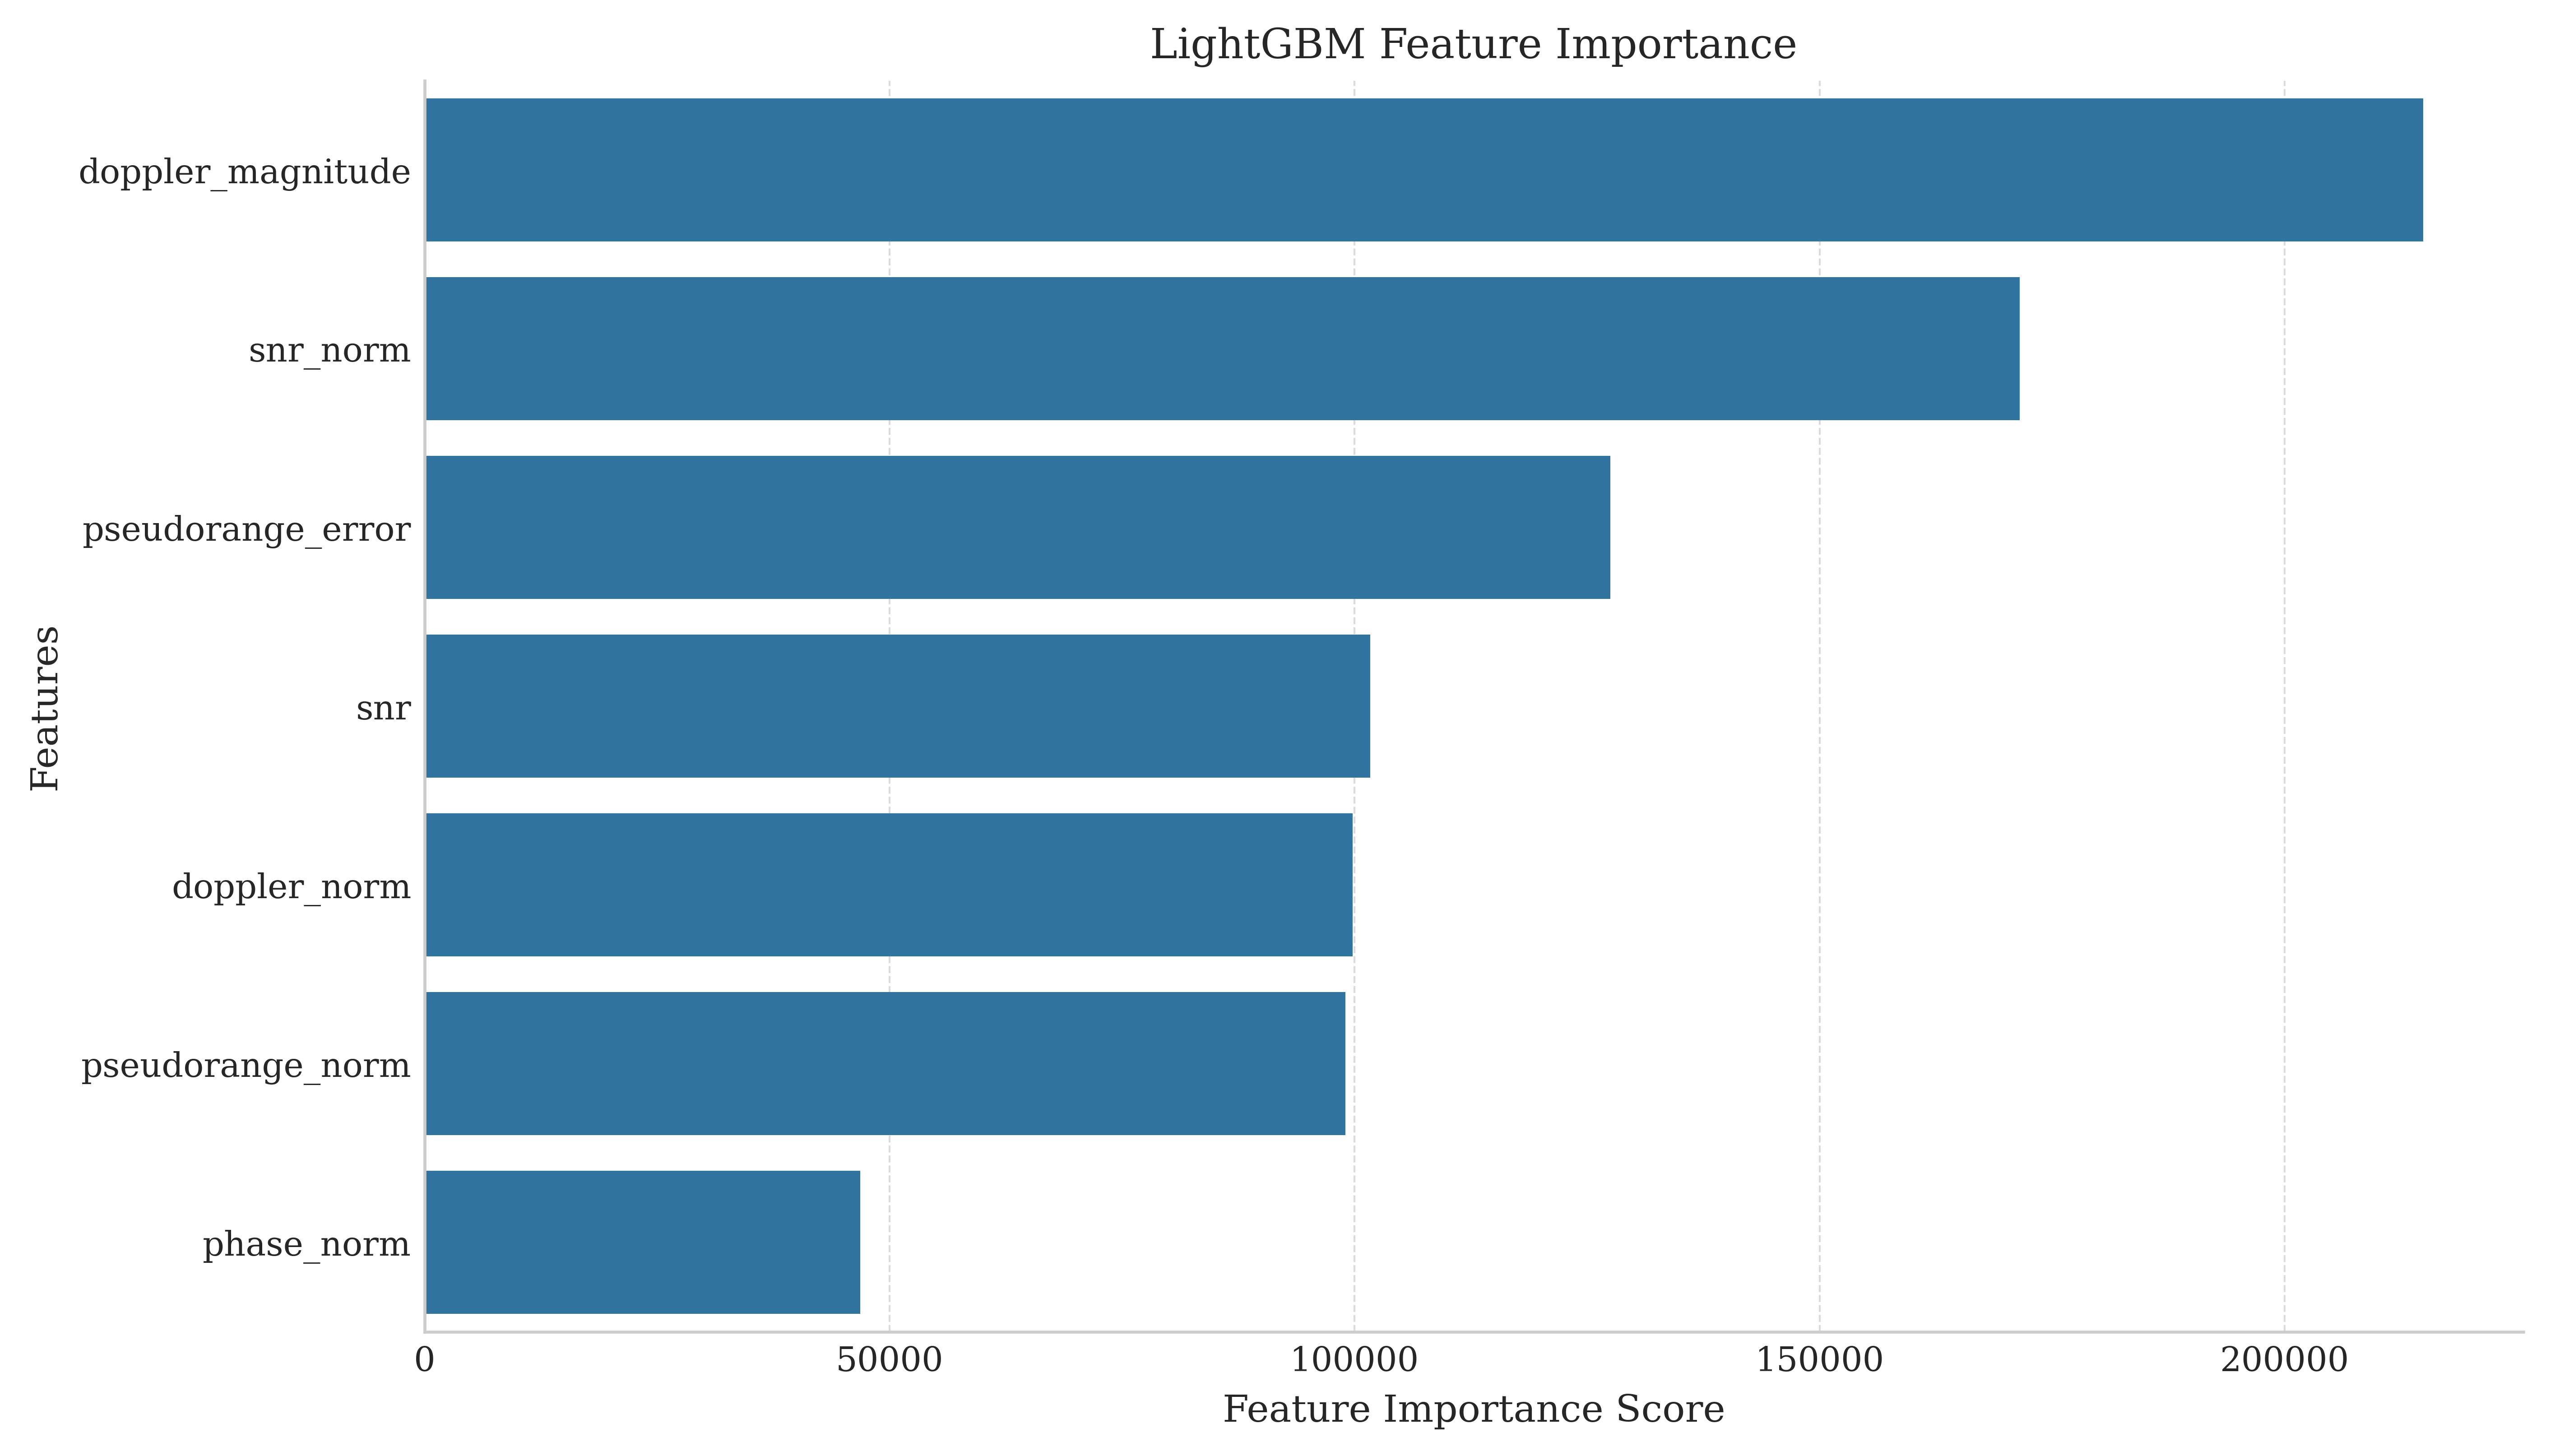
\includegraphics[width=1\textwidth]{Included_Images/feature_importance.png}
    \caption{Feature importance plot for LightGBM model}
\end{figure}
The figure indicates that the top three features for the LightGBM model are:
\begin{itemize}
    \item Doppler Measurement
    \item Carrier to Noise Ratio
    \item Pseudorange error
\end{itemize}
These features have the highest importance scores, indicating that they contribute significantly to the model's ability to classify
the signals accurately. This insight can be useful for future feature engineering and model improvement efforts.

\subsection{Prediction Confidence Analysis}
To further evaluate the performance of the model and the reliability of the predictions, a 
per satellite confidence analysis was conducted. The plot below shows confidence for the predictions
for some selected satellites. For each of the prediction, the model outputs a probability distribution. This is done
via the softmax function. The prediction confidence is defined as the maximum prediction probability. The calculation is done using the 
following equation:
\begin{equation}
    \text{Conf.}_i = \max_{k \in \{1,2,3\}} \; p_{i,k},
\end{equation}
here, the predicted probability of sample $i$ is denoted as $p_{i,k}$ which belongs to class $k$.
A confidence of 1 means a fully decisive prediction. A value near 0.33 reflects maximum uncertainty.
A threshold of 0.50 is set which is shown by the red dashed line. This threshold serves as a practical
unreliability mark. 
\begin{figure}[H]
    \centering
    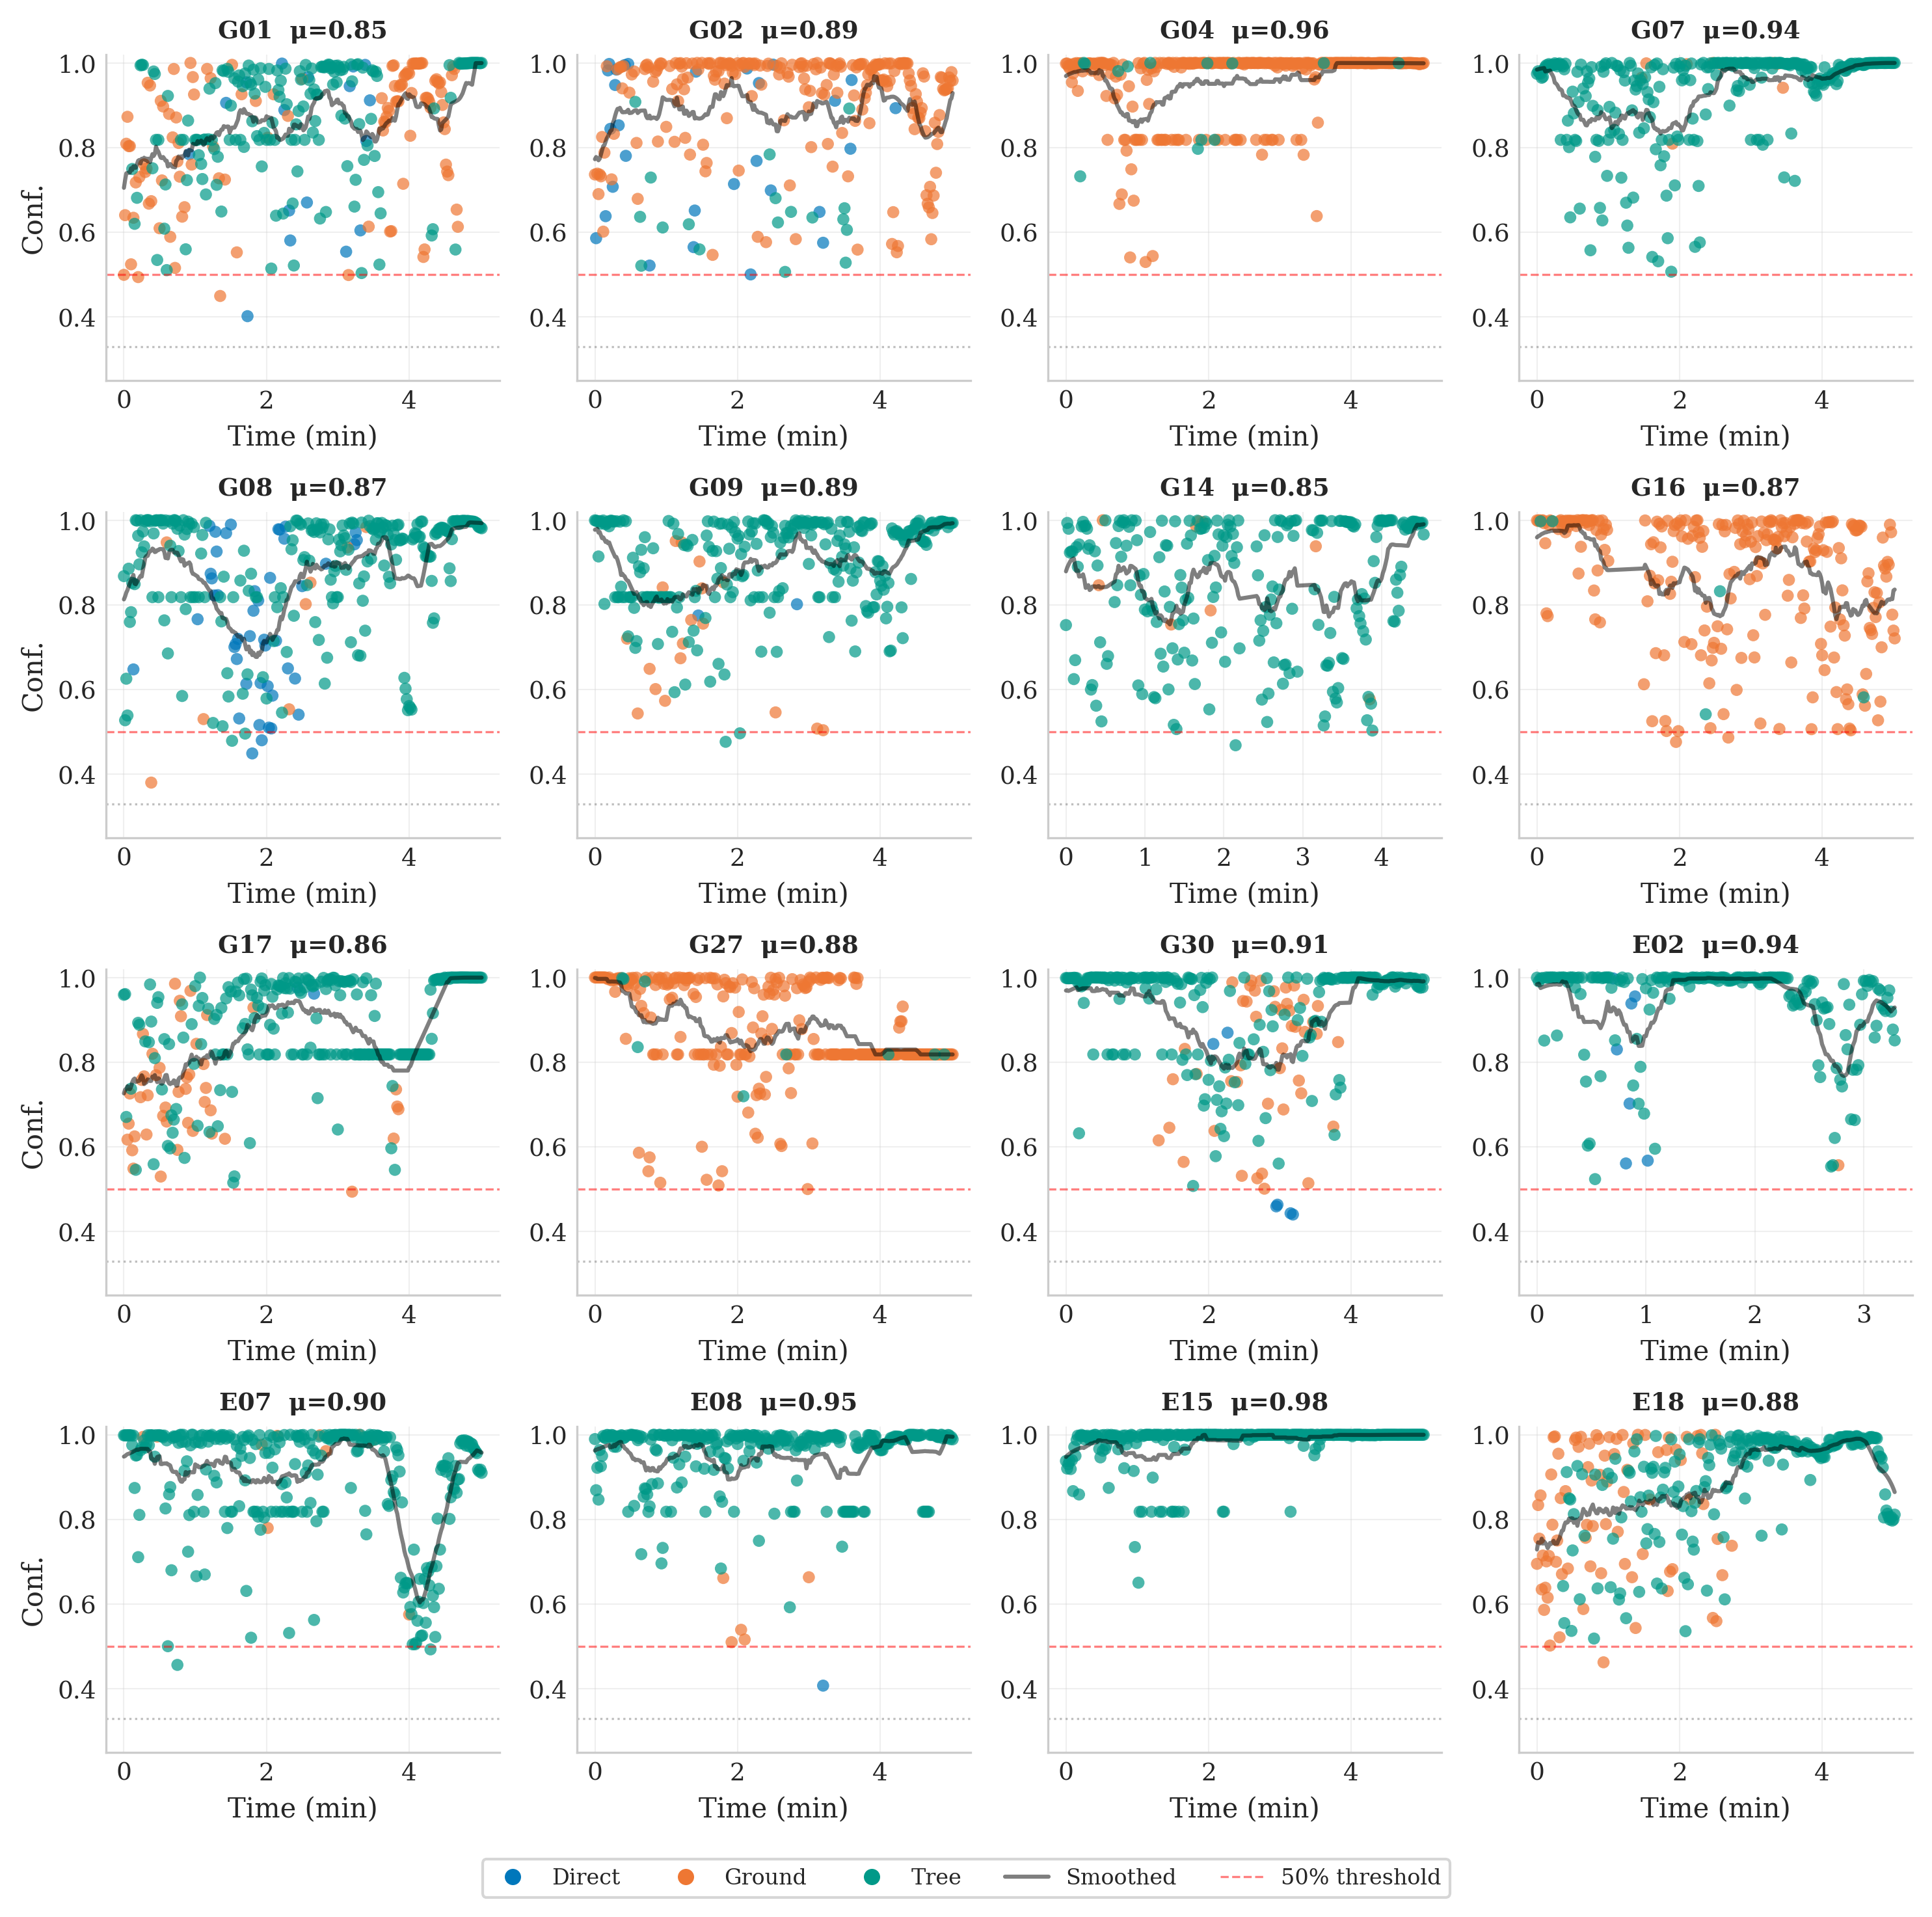
\includegraphics[width=0.7\textwidth]{Included_Images/confidence_timeseries_p1.png}
    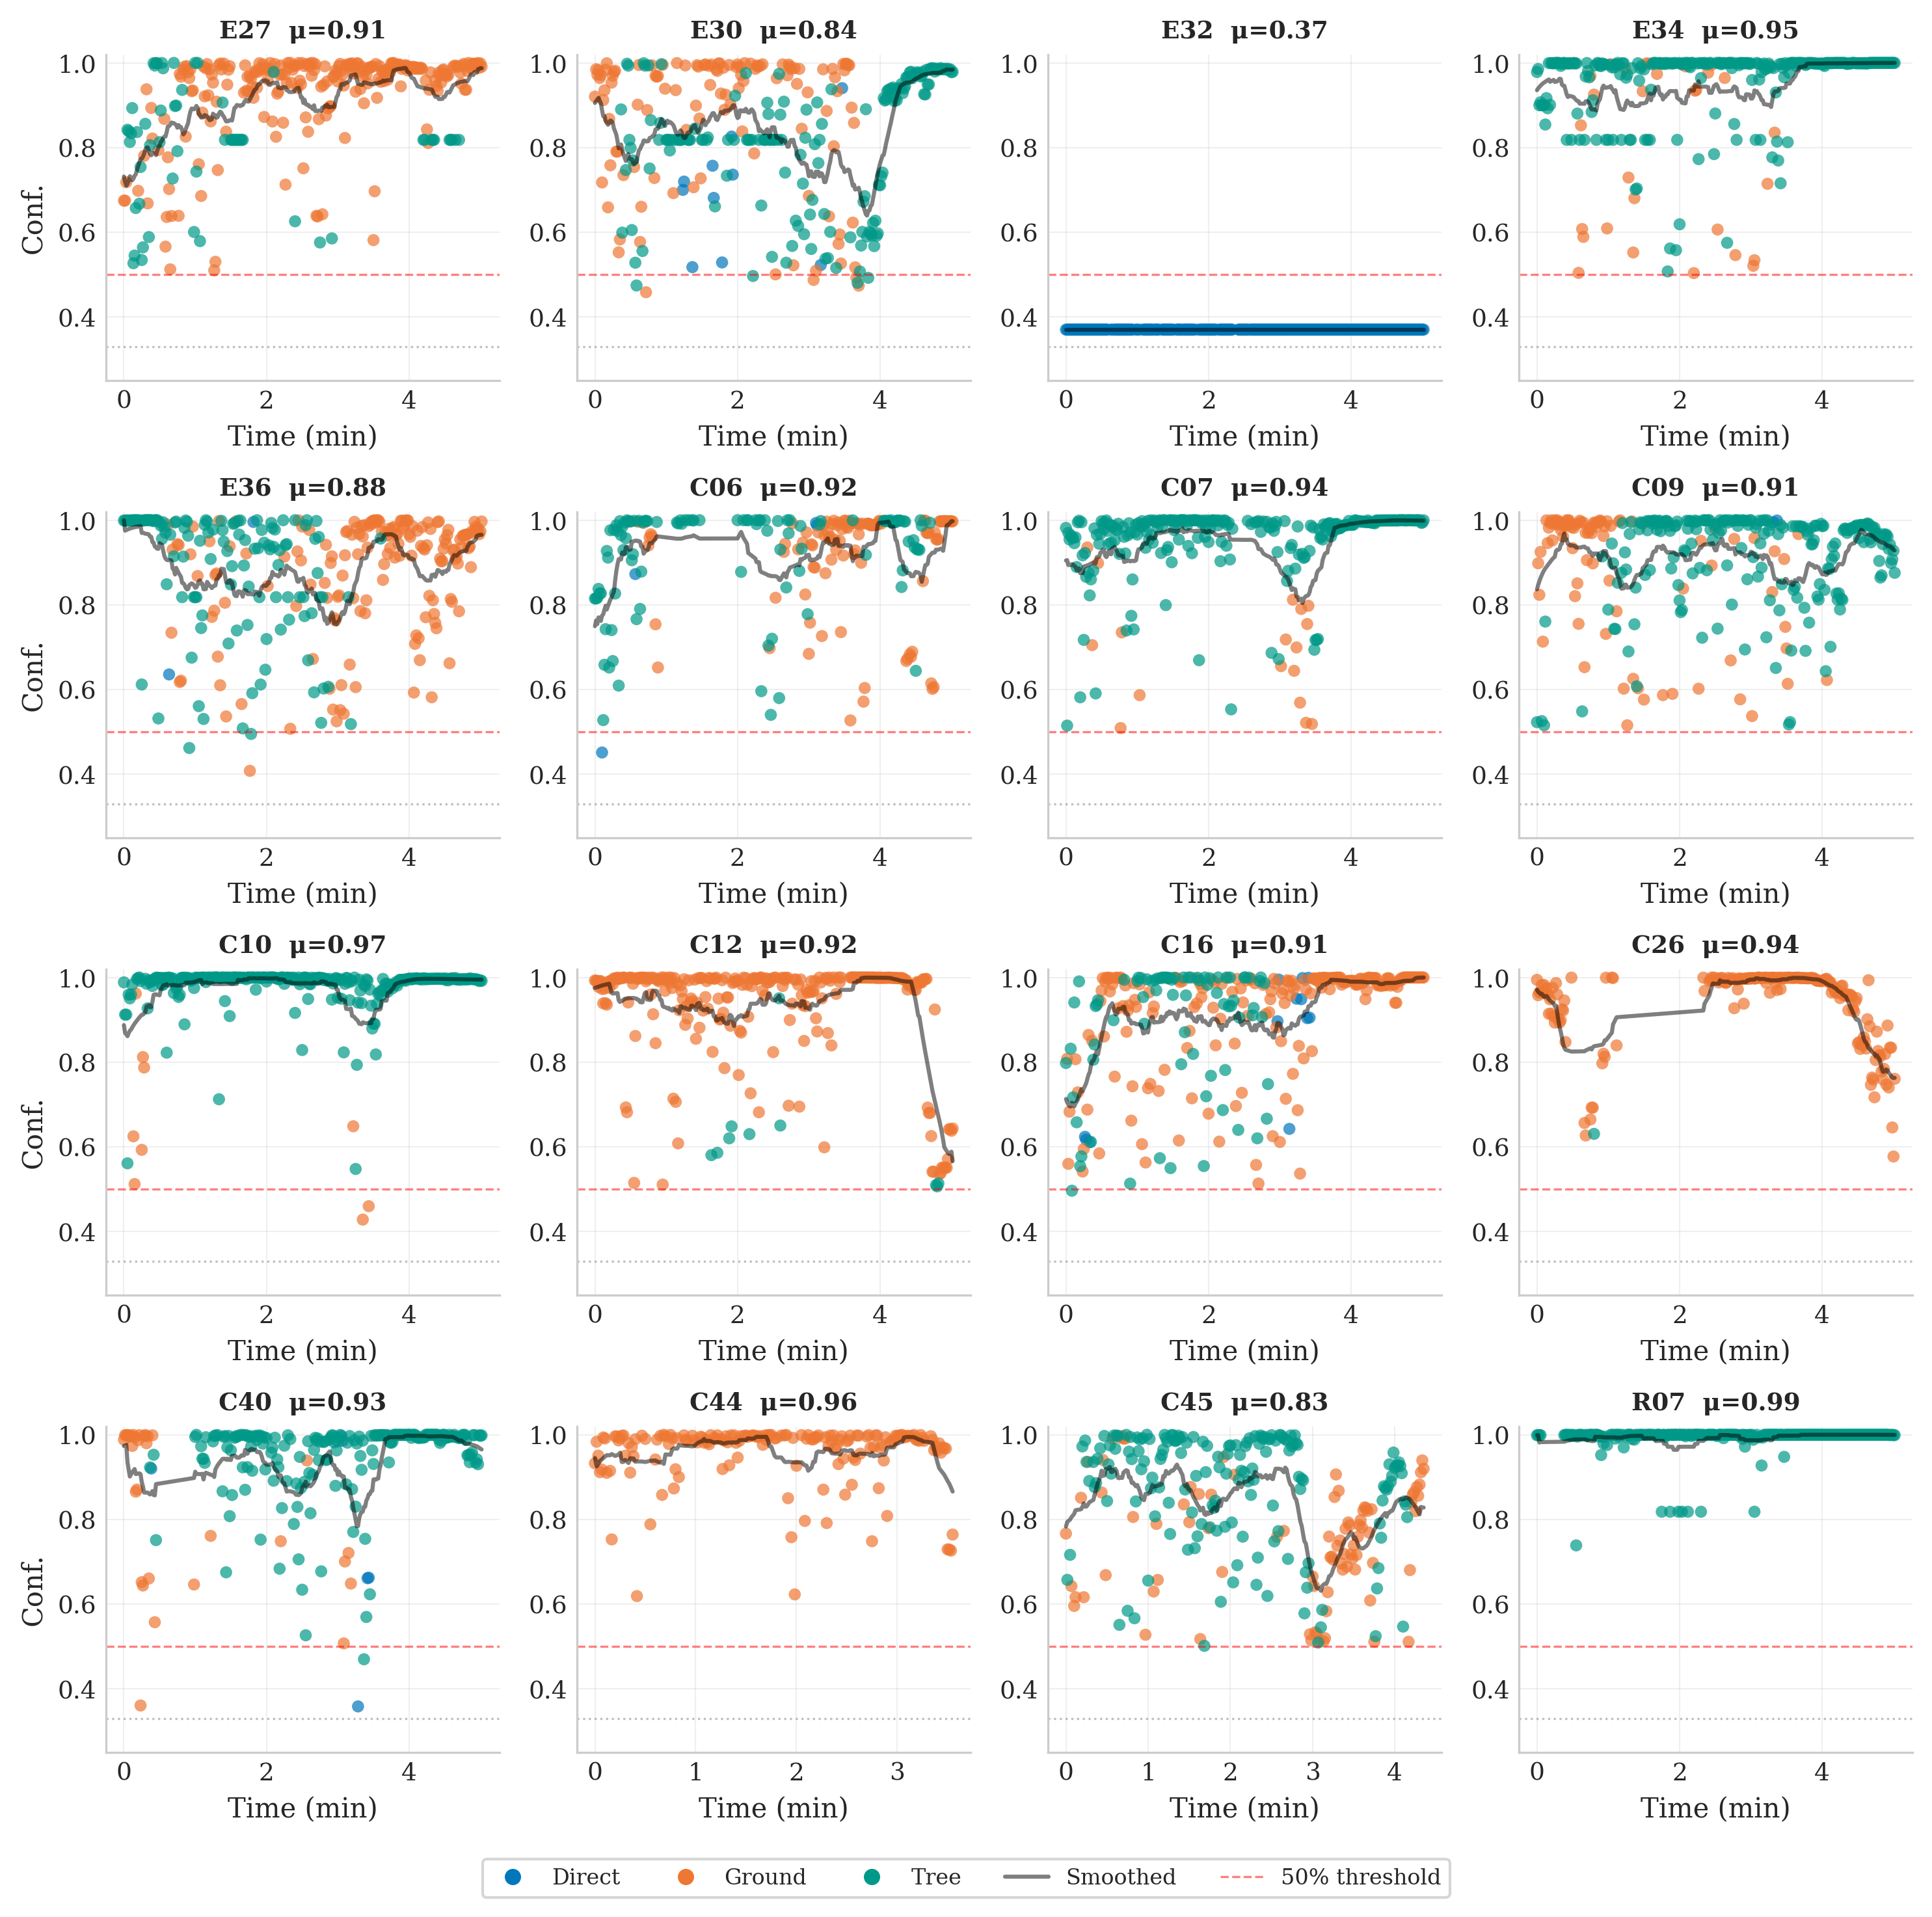
\includegraphics[width=0.7\textwidth]{Included_Images/confidence_timeseries_p2.png}
    \caption{Prediction confidence time series for selected satellites.}
\end{figure}



The figure above presents the confidence plot for some of the selected
satellites. The flight duration for this experiment was around 4.5-5 minutes. In
the plot, each of the dot reflects a measurement from that satellite and the
color reflects their predicted class. A blue colored dot represents a direct
signal, an orange dot reflects a ground reflected signal and lastly the green
dot represents the tree reflected signals. A smoothed confidence curve is also
plotted (in black) to represent the temporal trend. 

Across all 16 satellites the mean confidence ranges from 0.85 to 0.98. This indicates that the classifier 
consistently produces high confidence decisive predictions. Majority of the predictions lie above the threshold value. Galileo 
consistently tends to achieve slightly higher mean confidence than GPS which may be happening due to their consistent stronger signal quality.
A consistent feature of the predictions that can be observed from the plots is the dip around 1.5-2.5 minute mark. This is visible in the smoothed confidence curve 
for most of the satellites: G01, G02, G08, G14, G16, G17, G27, G30, E02, E18 etc. If closely examined, the curve dips first and then recovers towards 
higher confidence in the latter portion of the flight. During this dip, the scatter plots also show a higher degree of mixed predictions. This suggests that the model is 
temporarily uncertain about the signal class. This temporal uncertainty is likely happening due to a transition 
in the flight environment under the UAV. When the UAV flies between distinct terrain types the GNSS signal characteristic also changes that does not match clearly with the characteristic of any of the classes. 
During such transition, the feature values may exhibit mixed behaviors resulting in an uncertainty for the model. 
However, this uncertainty is a valuable insight for our project as one of the goals of the ML pipeline is to detect the vegetation boundary and the uncertainty exactly provides that information. 


\subsection{Vegetation Boundary Plotting and Analysis}
To provide a geospatial visualization of the vegetation boundary the prediction results were plotted on the map
of the experiment site which can be seen from the figure below. First, the FFZs for each of the satellite was calculated, and their centroids
were overlaid on a satellite map. The FFZ centroid can be assumed as a point which is dominant for reflections from a certain satellite and UAV altitude. 
In other words, it is the location on the ground where the reflections most likely originate from.
\begin{figure}[H]
    \centering
    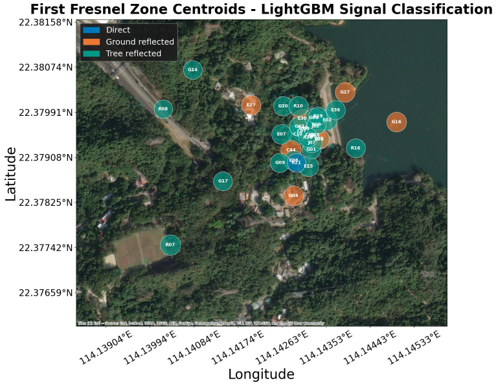
\includegraphics[width=1\textwidth]{Included_Images/Veg_boundary.png}
    \caption{Vegetation boundary plotting based on classified signals.}
\end{figure}

Each circle on the map represent a single satellites FFZ centroid which was enlarged by the mean confidence of the predictions. 
The color definition is same as the one for confidence plots, where blue mean direct, orange means ground reflected and green represents tree
reflected signals. The centroids are colored according to the most dominant prediction class of that satellite. Looking at the spatial distribution and the terrain, the 
predictions strongly align with the surface below. Satellites whose predictions fall over densely vegetated areas are predominantly classified as tree reflected signals. The same goes for the
other prediction classes. 

To further examine the spatial temporal relationship, two satellites are analyzed below.
\begin{figure}[H]
    \centering
    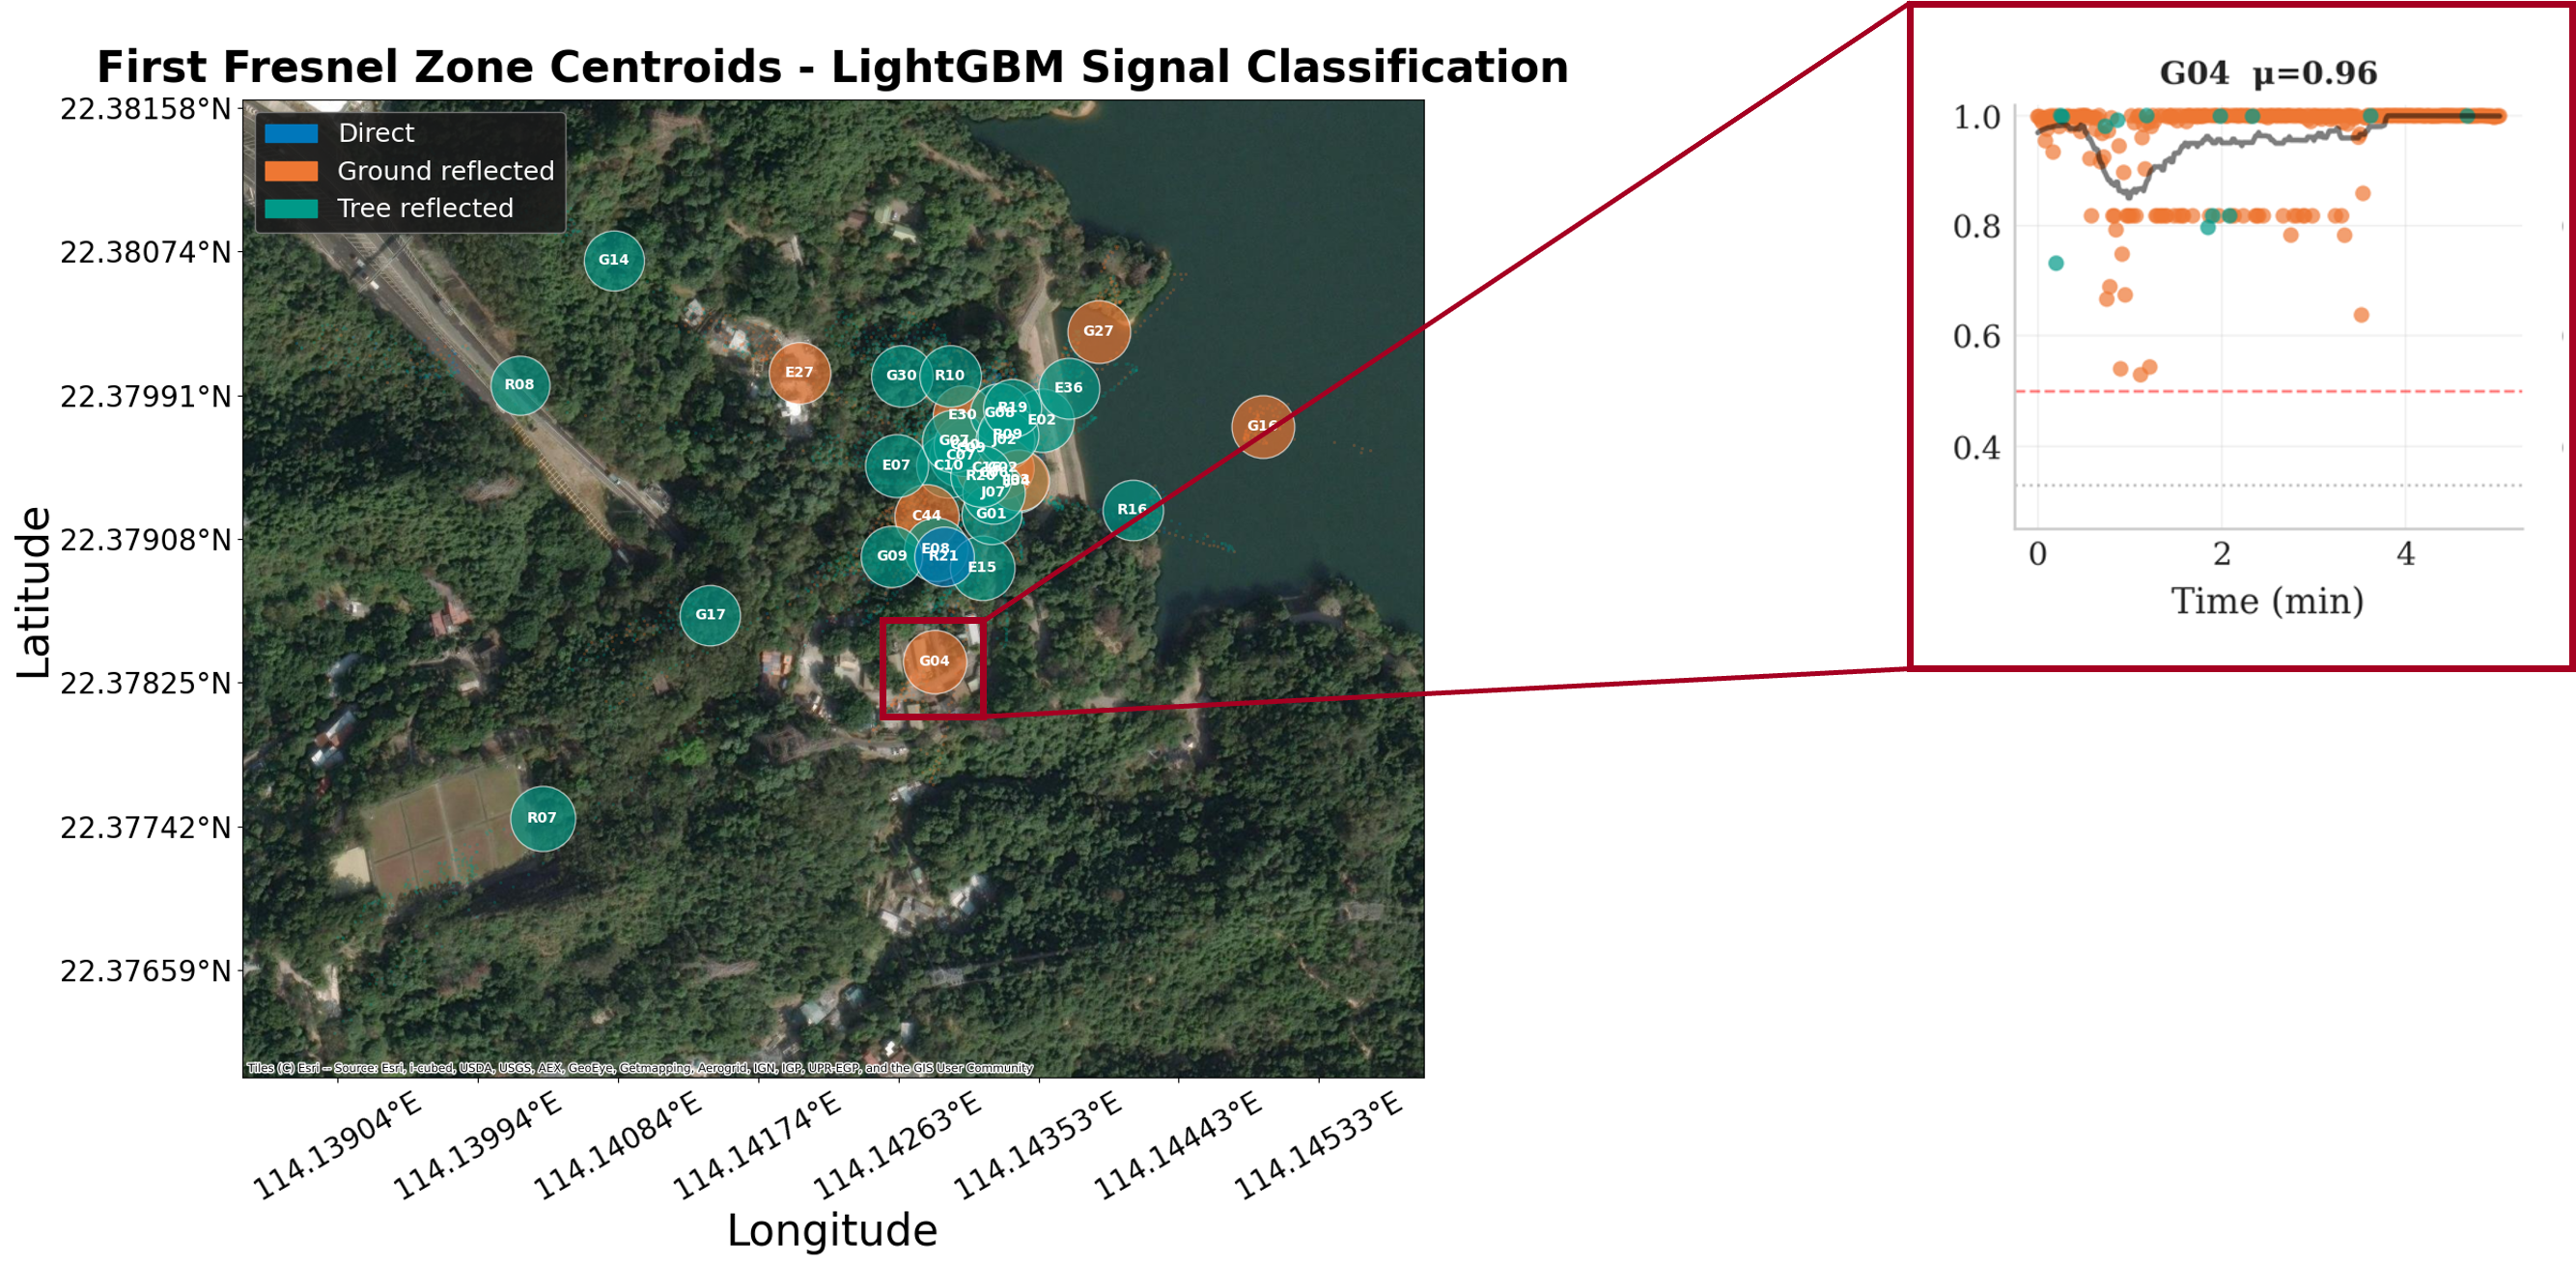
\includegraphics[width=1\textwidth]{Included_Images/veg_boundary_G04.png}
    \caption{Vegetation boundary plotting and G04 prediction confidence analysis.}
\end{figure}

The GPS satellite G04's FFZ centroid is positioned at a place that can be identified as bare ground. The confidence plot for G04 indicates that the
predictions also converge quickly after the flight and remain stable. The dominant prediction class is observed to be ground reflected signal class (orange). The 
class received near unity confidence beyond the 1-minute mark. The first minute is observed to slightly uncertain which might be due to unsettling geometry of the reflection when the UAV was
moving to its operating altitude. However, once stabilised the model predicts the measurements to be ground reflection with a consistent confidence of 0.8-1. 
The high mean confidence and a single class prediction demonstrates that the classifier correctly predicts the signal class or type when the FFZ falls over a clear and unambiguous terrain. 
\begin{figure}[H]
    \centering
    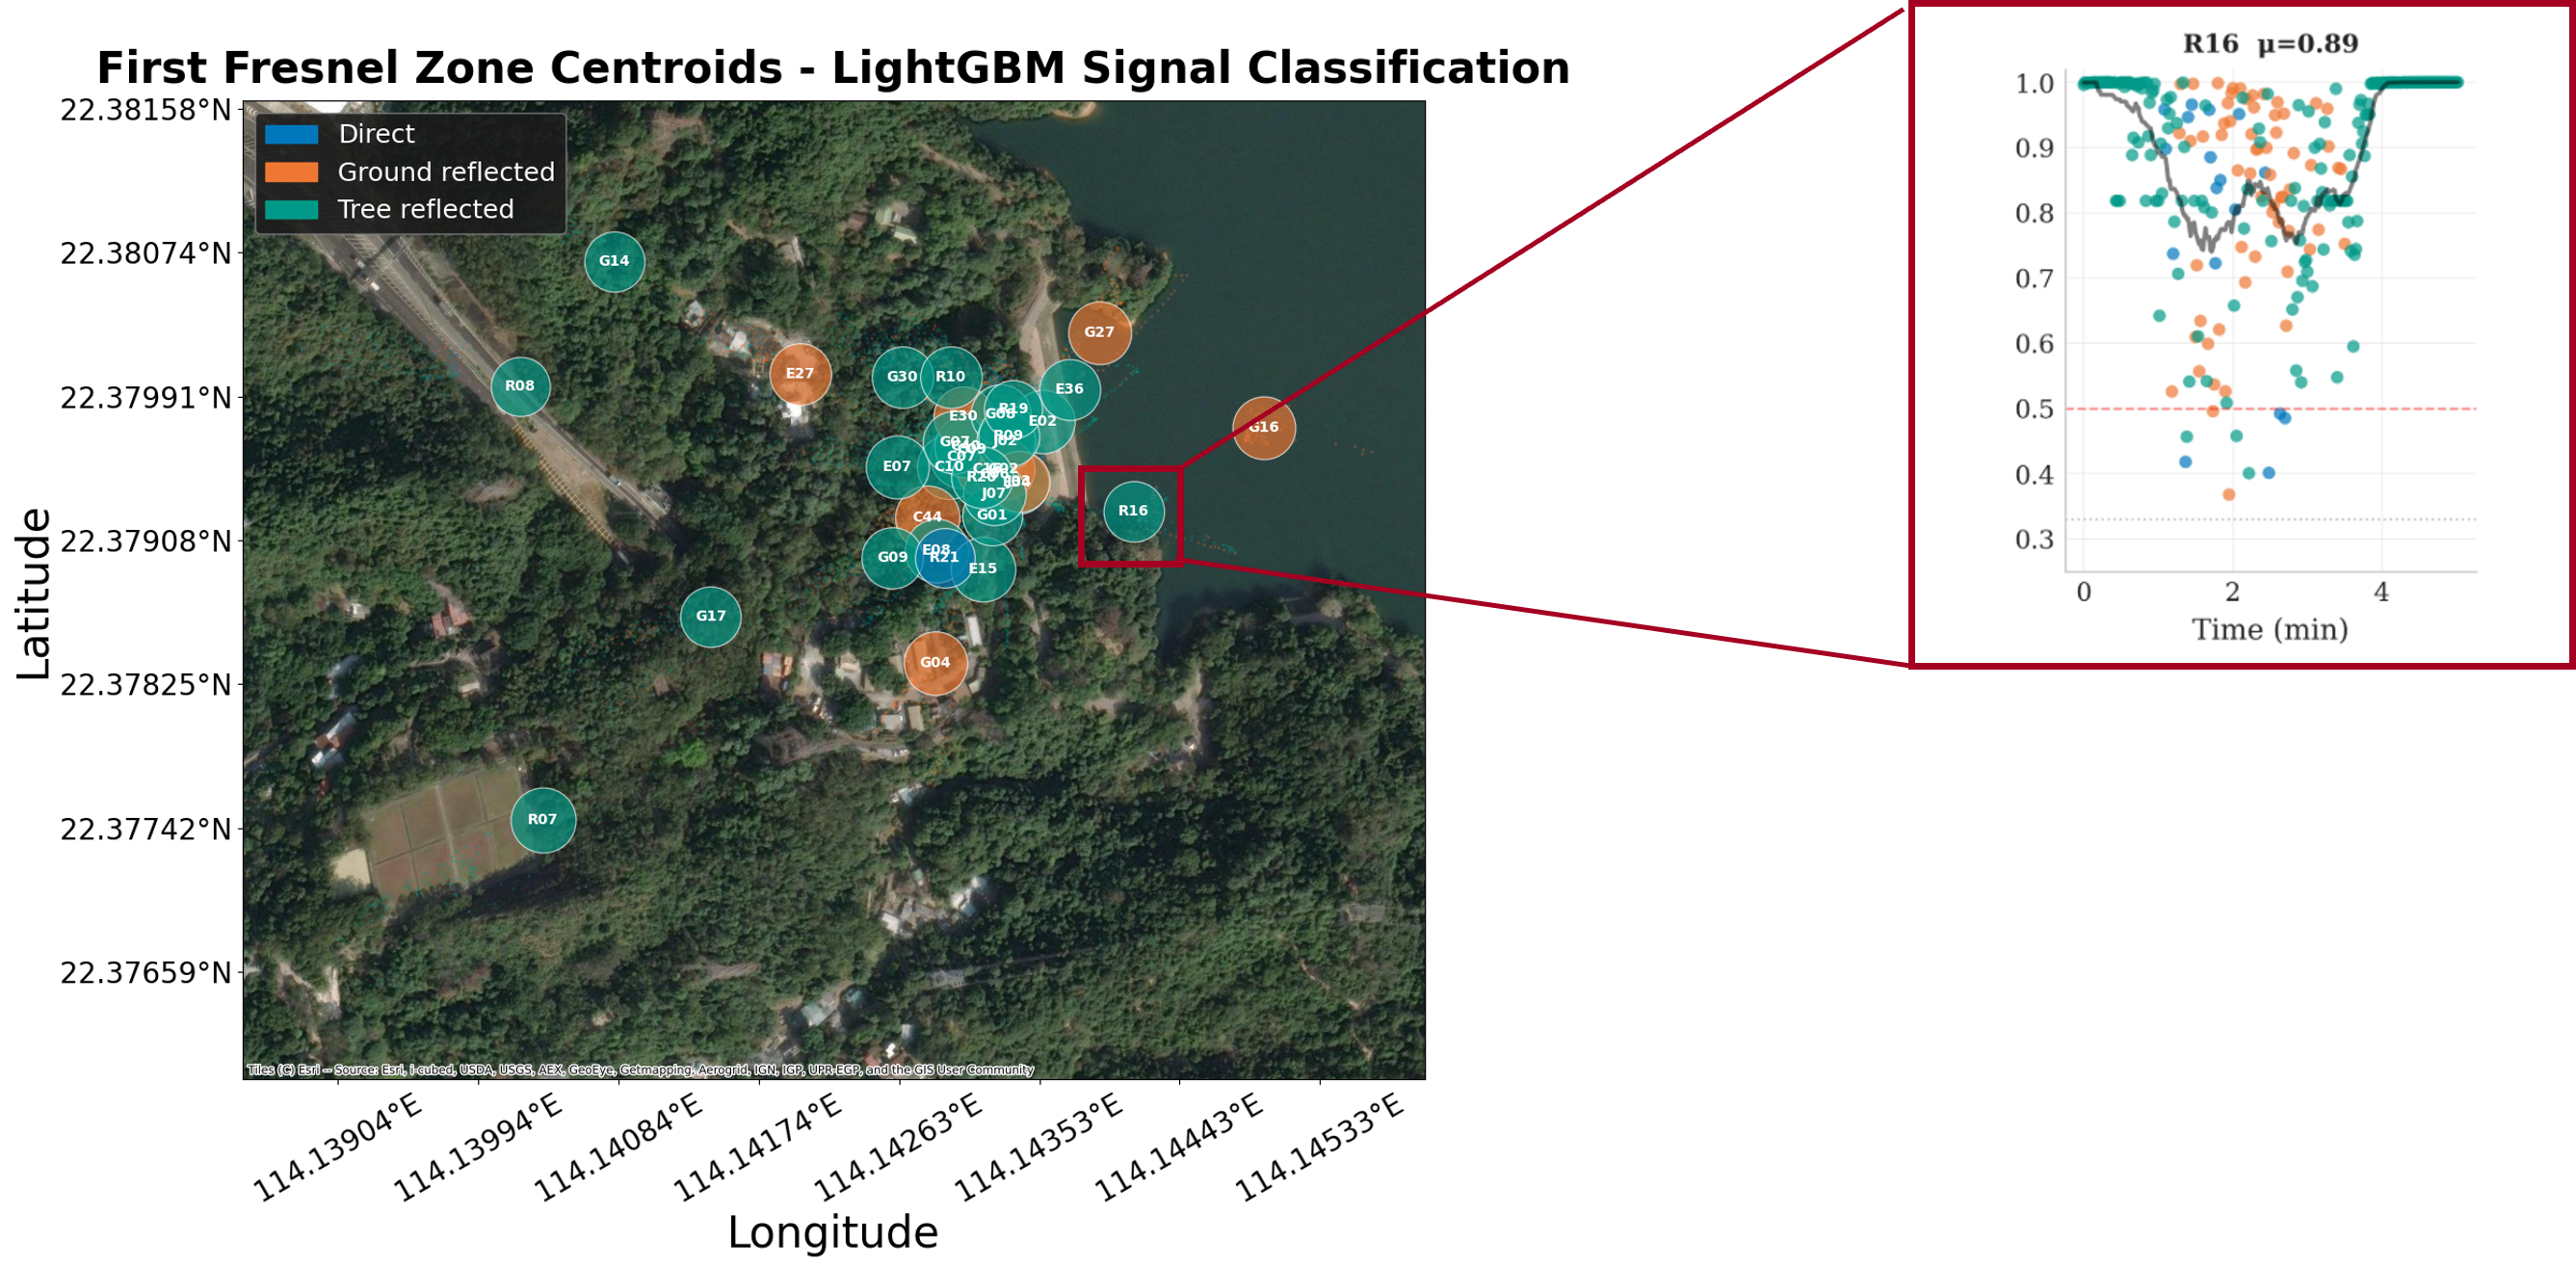
\includegraphics[width=1\textwidth]{Included_Images/veg_boundary_R16.png}
    \caption{Vegetation boundary plotting and R16 prediction confidence analysis.}
\end{figure}

However, if we examine the FFZ centroid location of R16, it is comparatively a challenging environment. The centroid
of the FFZ for this satellite is located near the shoreline where a transition can be seen from water to vegetation.
The signal characteristic is expected to be mixed in this region due to the underlying terrain. And it is also evident if you closely
examine the confidence plot for this specific satellite. The confidence is high in the opening minute with reflection types predominantly
classified as tree reflected signals. However, a severe dip is noticed between the timestamp for 2-3.5 minutes. During this time, the confidence 
collapses to as low as 0.3 which is below the threshold. This is consistent with the FFZ centroids movement near the terrain boundary. As the UAV moves the FFZ and the satellite 
geometry also changes. This naturally means the same signal gets reflected from different surfaces throughout the flight. After the 3.5 minute mark, the prediction confidence
stabilizes and recovers to near 1 value with tree reflected predictions. This suggests the reflection geometry has moved back to vegetation zone.

\begin{figure}[H]
    \centering
    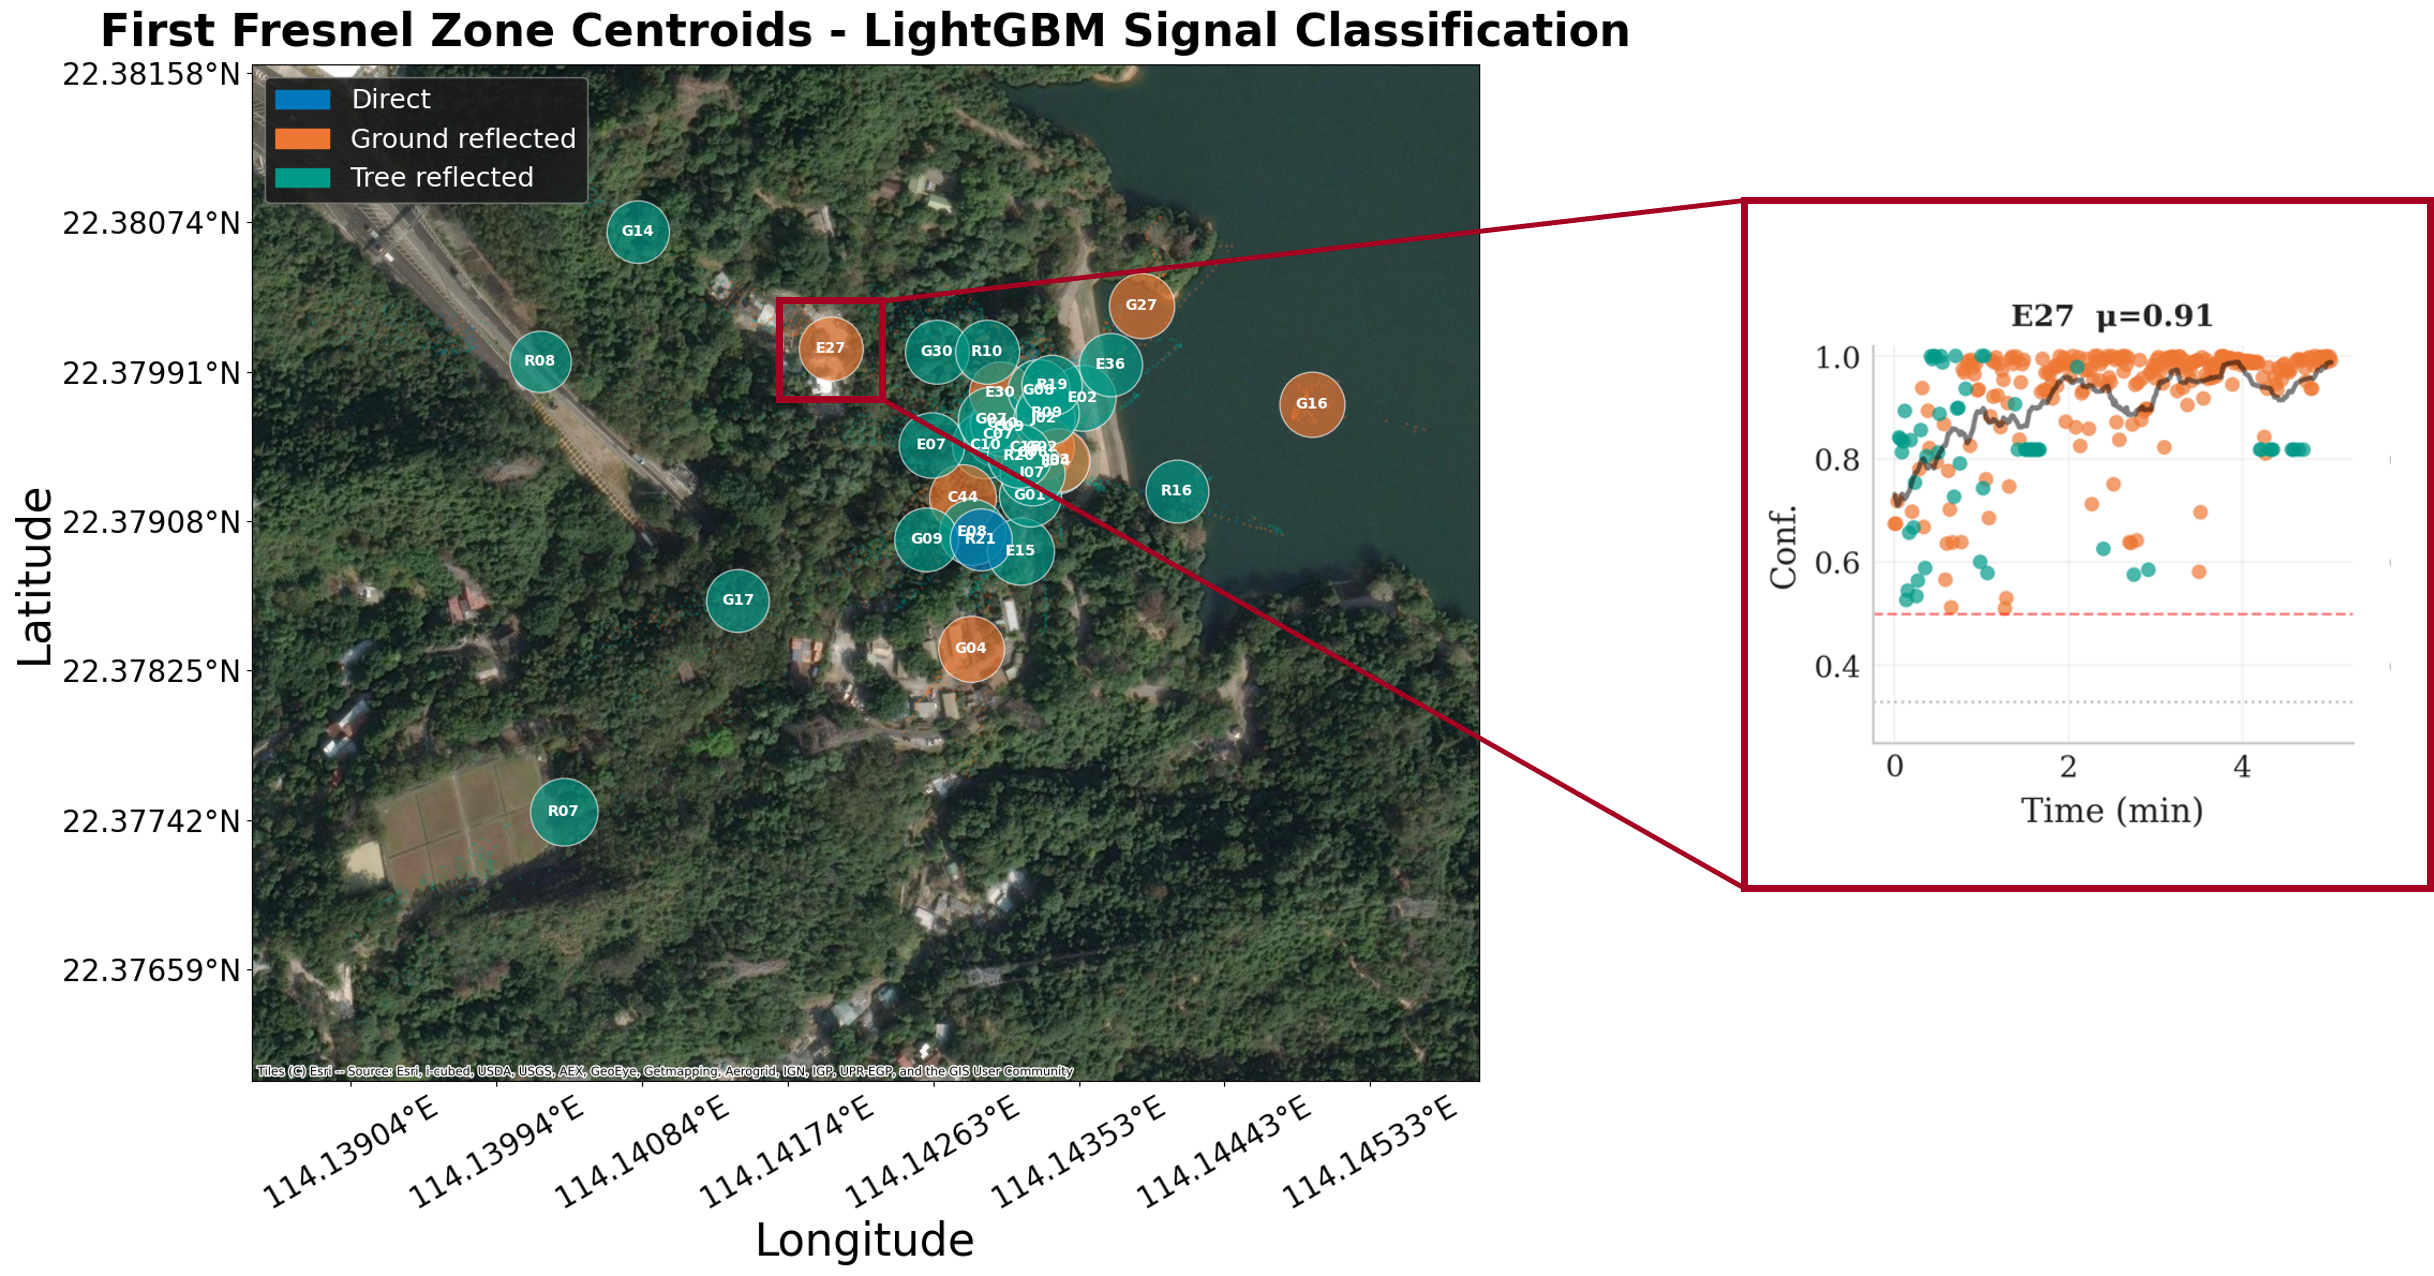
\includegraphics[width=1\textwidth]{Included_Images/veg_boundary_E27.png}
    \caption{Vegetation boundary plotting and E27 prediction confidence analysis.}
\end{figure}

Satellite E27 also has its centroid near a boundary transition zone. It can be seen from the terrain on the map 
that the centroid falls near the transition zone between bare ground and trees. And it is also observed from the confidence plot
for this satellite. The confidence plot shows that the confidence in the first 1-1.5 minute is around 0.6-0.85 with
mixed predictions of tree reflected and ground reflected signals. This early ambiguity is consistent with the edge location of the FFZ where the 
reflection initially might be coming from both vegetated and open terrain. However, after 2 min mark, the confidence and the prediction pattern changes. The confidence
stabilizes with a value of over 0.9. The prediction class is also found to be dominantly ground reflected. E27 thereby represents an intermediate case between the stable high confidence behavior 
of G04 and severe confidence dips of R16. This satellite also strengthens the fact that the prediction confidence lowers near the boundary transition zones making the confidence dips an important observation
for vegetation boundary construction.

So to conclude, the three cases illustrate the relationship between the terrain type and the prediction confidence. 
Satellites with points of reflection that are on a uniform terrain result in constant, high-confidence 
predictions over the flight. But those close to terrain boundaries have 
temporary uncertainty which is to be explained physically not to denote 
model failure.
% --- Experiments ---
\section{Experiments}
In this project, an extensive series of field experiments were conducted, aiming
to demonstrate the functionality of the UAV platform and collect the data
necessary for further analysis. Over twenty unique flight missions were executed
across three different locations in Hong Kong and diverse flight scenarios,
including static hovering, dynamic surveying, and manually controlled flight.
The following subsections present the experimental setups and summarize the
experiments conducted.

\subsection{Experimental Setup}
Before the initiation of a flight mission, the ground control station must be
configured and remote connections with the onboard computer should be established.

\subsubsection{Ground Control Setup}
To set up the ground control station, the 433 MHz radio telemetries are first
paired up to establish remote connection between the onboard controller and the
ground control computer. This is facilitated through the QGroundControl (QGC)
software, which is a full-featured flight control and mission planning platform
for MAVLink-enabled drones \cite{QGroundControl_PlanView}. For all the
non-manual flights conducted, QGC is used to set up and execute flight missions,
where a set of waypoints could be selected in the plan view, including takeoff
and landing positions (Figure \ref{fig:qgc_plan_view}).

In addition to the waypoint locations, the altitude and speed at each waypoint
will be specified through the mission command list to meet the mission
requirements. For instance, for hovering missions, a speed of 2 m/s will be
assigned, where the UAV will be instructed to hold its position at the specific
waypoint for a specified period of time. Figure \ref{fig:qgc_mission_list} shows
an example of a mission command list in QGC.

\begin{figure}[H]
    \centering
    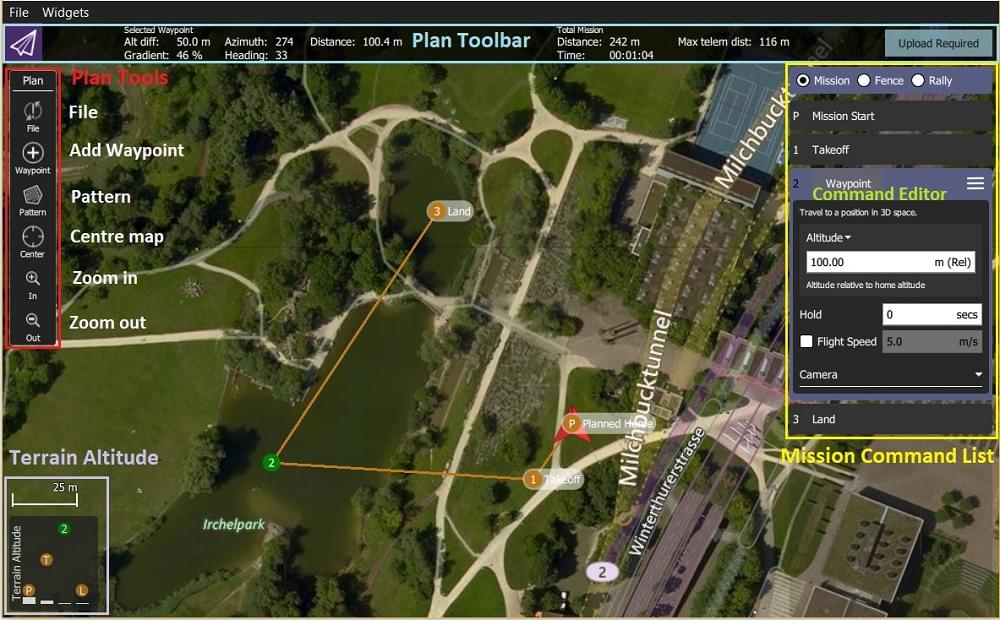
\includegraphics[width=0.8\textwidth]{Included_Images/qgc_planview.jpg}
    \caption{QGroundControl Plan View}
    \label{fig:qgc_plan_view}
\end{figure}

\begin{figure}[H]
    \centering
    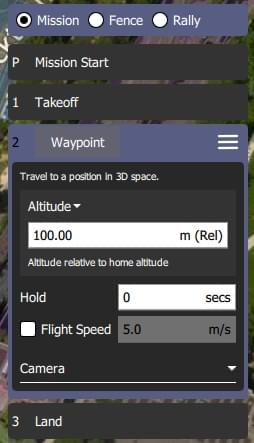
\includegraphics[width=0.4\textwidth]{Included_Images/qgc_mission_list.jpg}
    \caption{QGroundControl Mission Command List}
    \label{fig:qgc_mission_list}
\end{figure}

\subsubsection{Establishing Remote Connection with Onboard Computer}
While the ground controller is being set up, the onboard Jetson Orin is connected
through both the SSH protocol and remote desktop on two separate computers. 

Through Wi-Fi, both the SSH computer and the Jetson Orin are connected to a
common internal network that was pre-established using ZeroTier. The terminal of
the Jetson Orin can be accessed through Visual Studio Code, where the command to
log GNSS data from the two onboard receivers can be executed. 

On the other hand, SLAM data including LiDAR point clouds, IMU, and GPS data are
collected into a .bag file from Robot Operating System (ROS). To do so,
Nomachine is used to create remote access to the Jetson Orin with the
pre-established ZeroTier connection. This method enables access to multiple
terminals from Jetson Orin so that all the required sensor drivers can be
launched to carry out data collection.

With the trajectory plan uploaded onto the onboard Pixhawk controller and the
onboard computer configured to initialize data collection, the mission could be
executed. Ultimately, the collected data is downloaded and post-processed for
further analysis.

\subsection{Summary of Experiments Conducted}
A total of 24 successful mission flights were conducted for this project. They
were carried out in five locations: Homantin Mountain, Tai Hang Tun Kite Flying
Area, Nam Sang Wai, Mount Davis Service Reservoir Garden, and Upper Shing Mun
Reservoir Barbecue Area. Photos showing the experiment locations are arranged in
Figure \ref{Experiment Environment} and the experiments are summarized in Table
\ref{Experiment-Summary}.

\begin{figure}[H]
    \centering
    \begin{subfigure}{0.32\textwidth}
        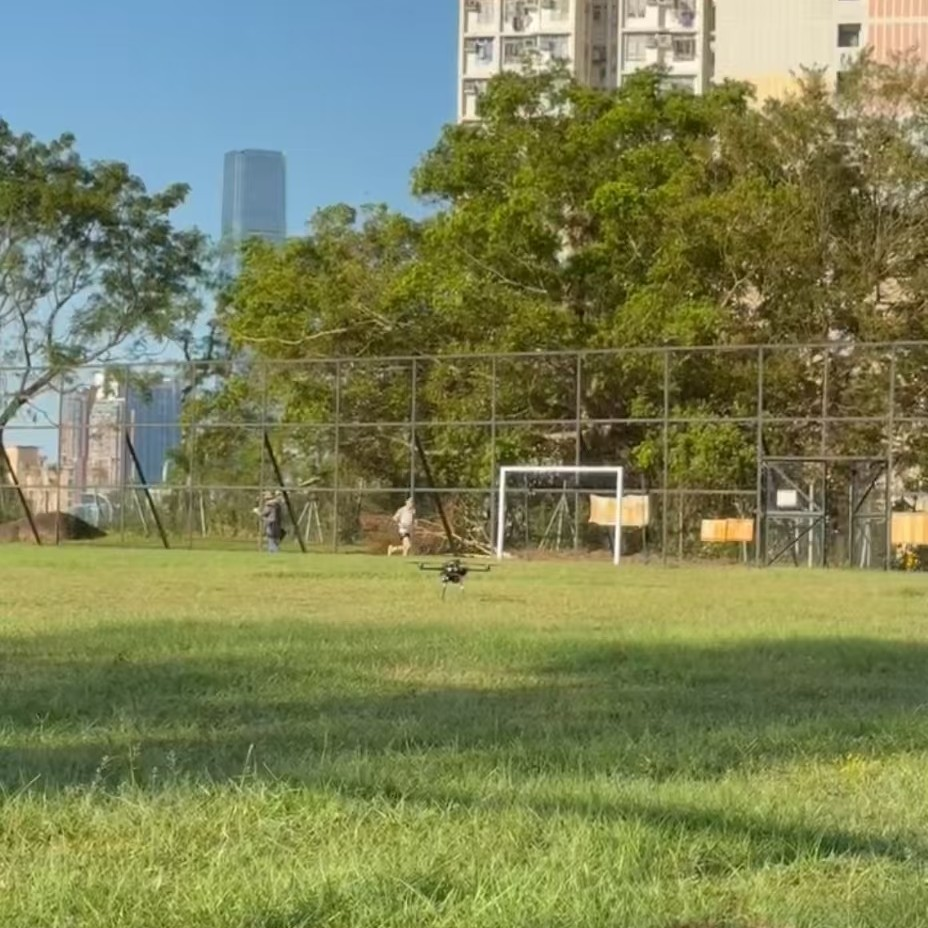
\includegraphics[width=\linewidth]{Included_Images/HomantinMountain.jpg}
        \subcaption{Homantin}
    \end{subfigure}
    \hfill
    \begin{subfigure}{0.32\textwidth}
        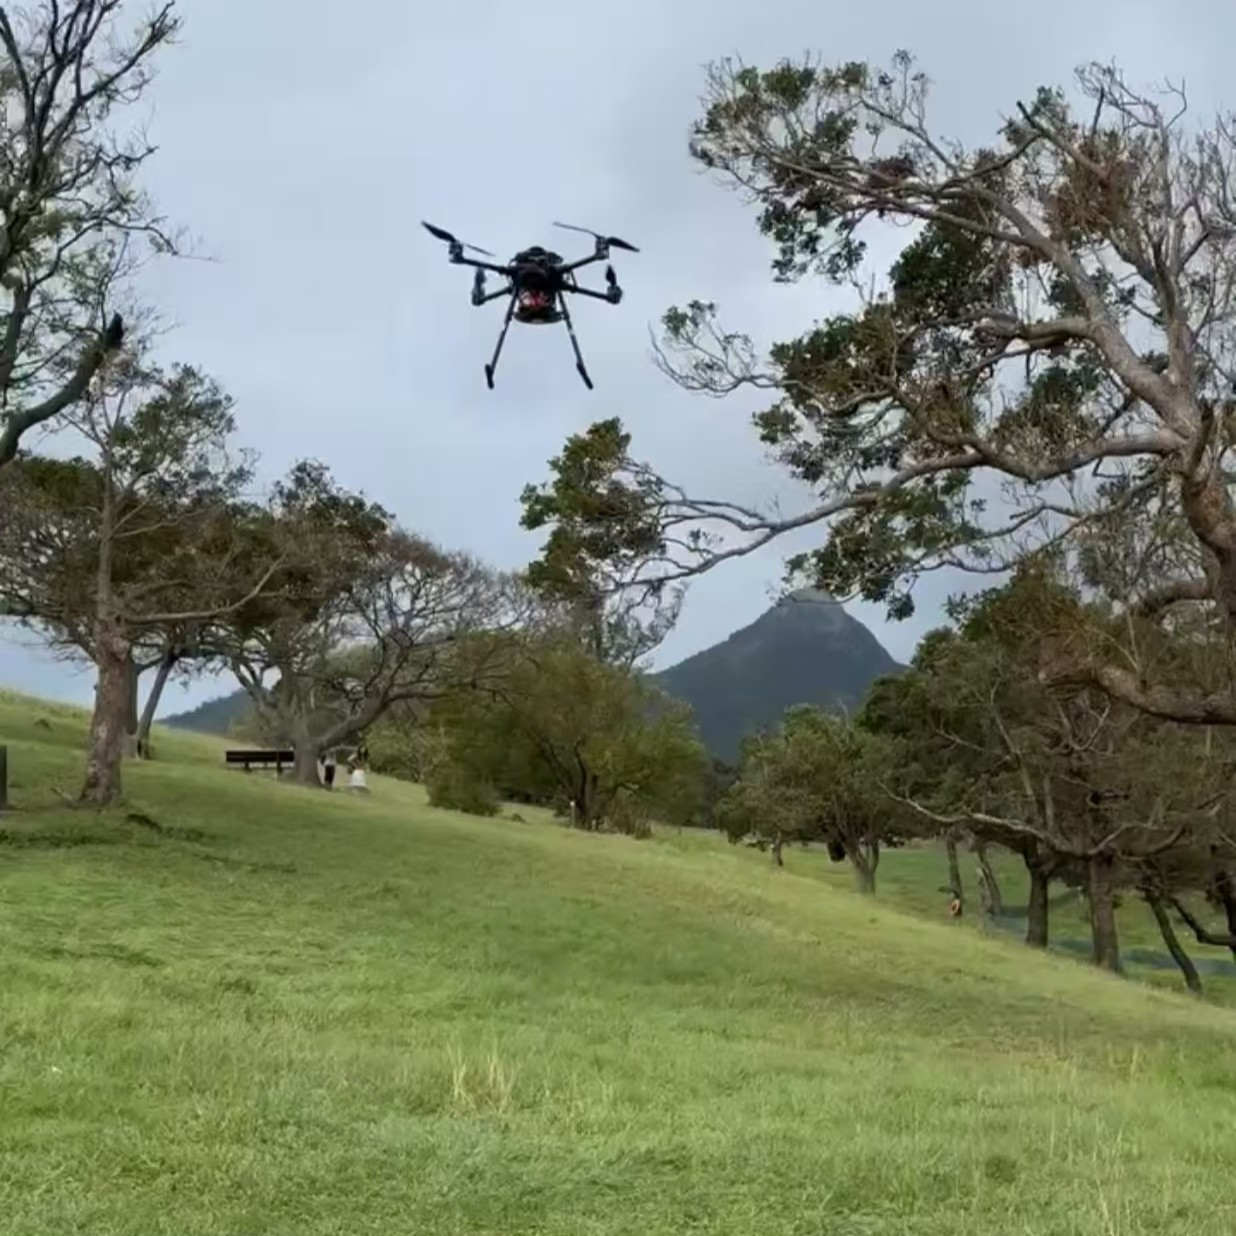
\includegraphics[width=\linewidth]{Included_Images/TaiHangTun.jpg}
        \subcaption{Tai Hang Tun}
    \end{subfigure}
    \hfill
    \begin{subfigure}{0.32\textwidth}
        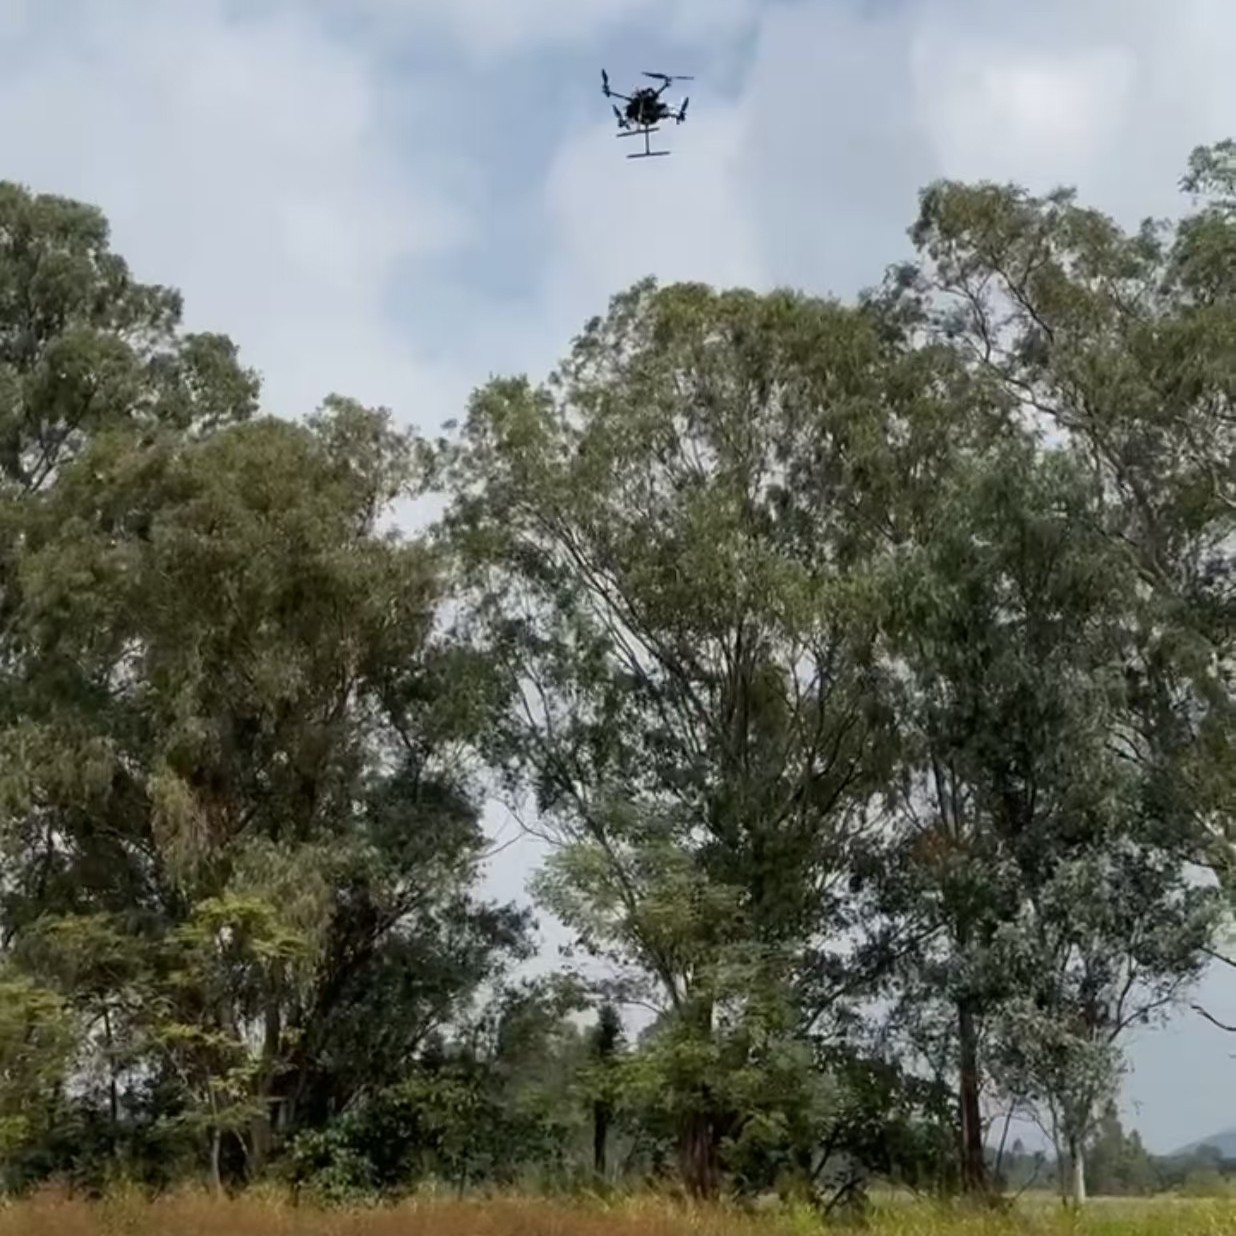
\includegraphics[width=\linewidth]{Included_Images/NamSangWai.jpg}
        \subcaption{Nam Sang Wai}
    \end{subfigure}
    \vfill
    \begin{subfigure}{0.32\textwidth}
        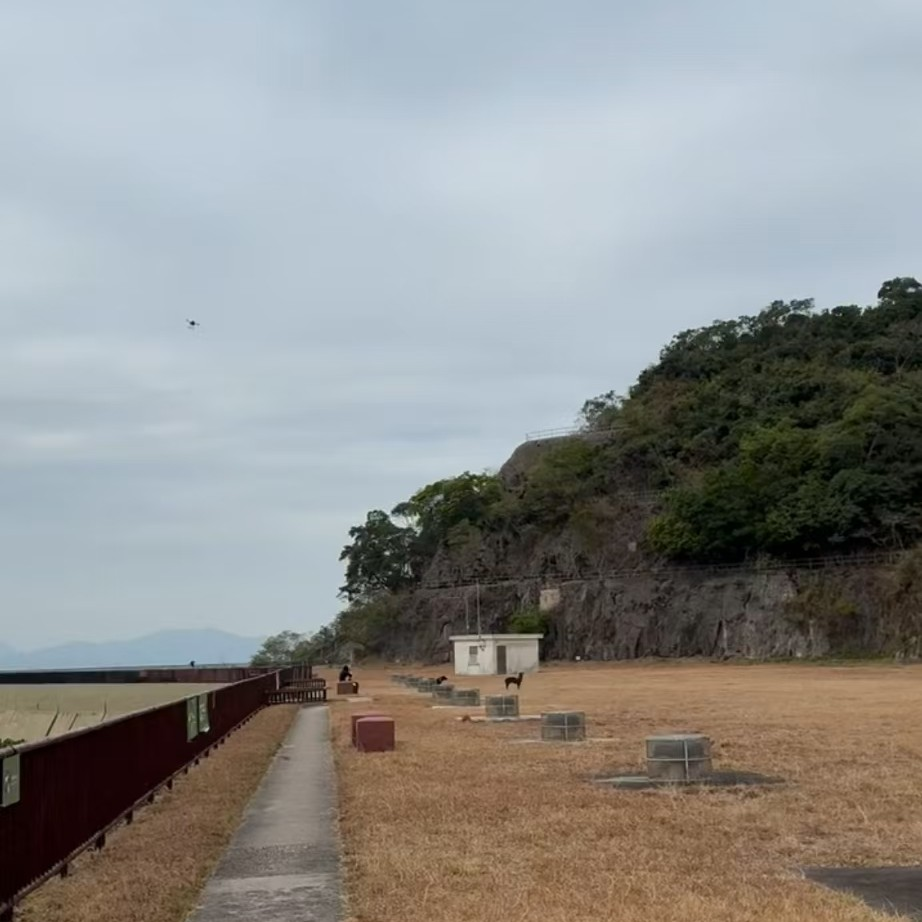
\includegraphics[width=\linewidth]{Included_Images/MtDavis.jpg}
        \subcaption{Mount Davis}
    \end{subfigure}
    \hspace{0.02\textwidth}
    \begin{subfigure}{0.32\textwidth}
        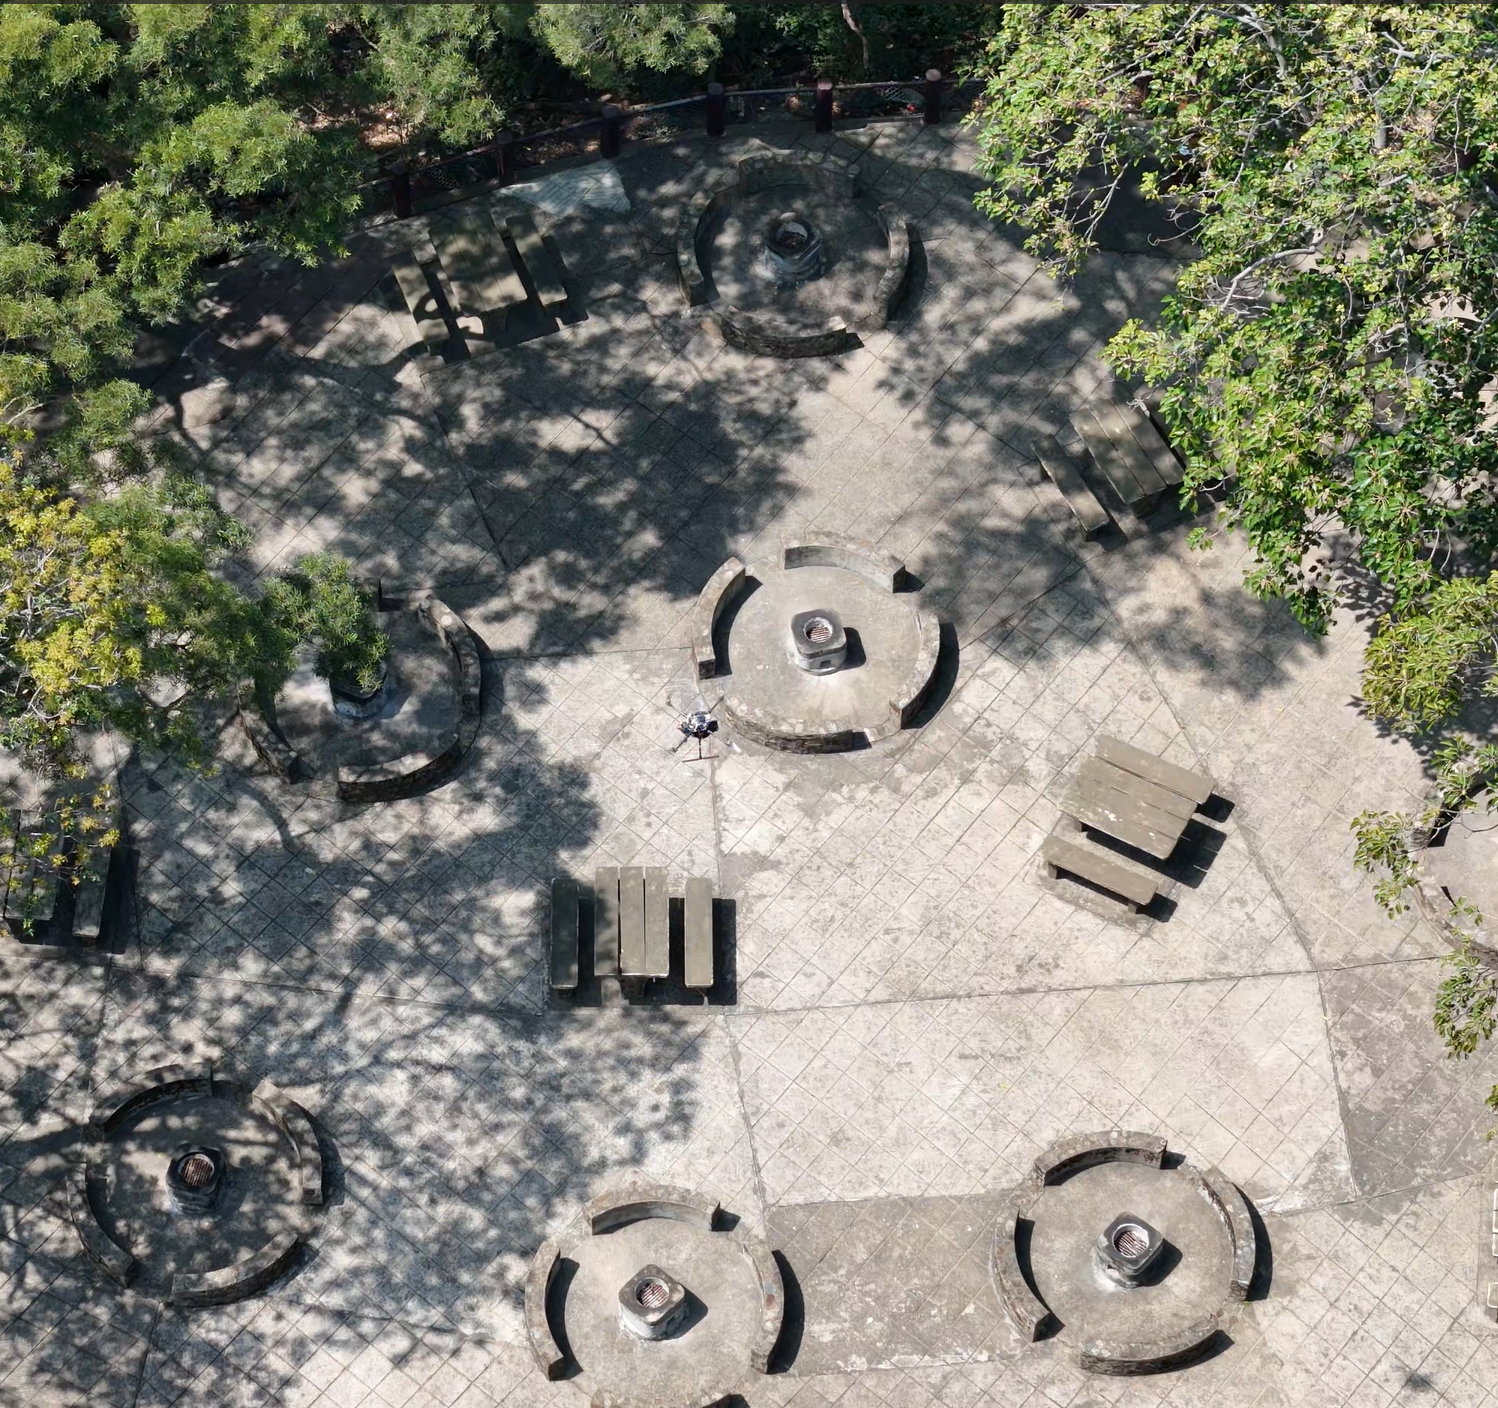
\includegraphics[width=\linewidth]{Included_Images/Shingmun.png}
        \subcaption{Shing Mun}
    \end{subfigure}
    \caption{Experiment environment photos at experiment locations.}
    \label{Experiment Environment}
\end{figure}

\begin{tabularx}{\textwidth}{|m{0.03\textwidth}|m{0.05\textwidth}|m{0.1\textwidth}|>{\raggedright\arraybackslash}X|>{\centering\arraybackslash}X|}
    \caption{Summary of Experiments Conducted}
    \label{Experiment-Summary}\\
    \hline
    & \textbf{Date} & \textbf{Location} & \textbf{Description} & \textbf{Flight
    Trajectory}\\ 
    \hline
    \endfirsthead
    \hline
    & \textbf{Date} & \textbf{Location} & \textbf{Description} & \textbf{Flight
    Trajectory}\\ 
    \hline
    \endhead
    \hline
    \endfoot
    (a) & 2025 Oct. 01 & Homantin & Manual flight over bare ground with grass. &
    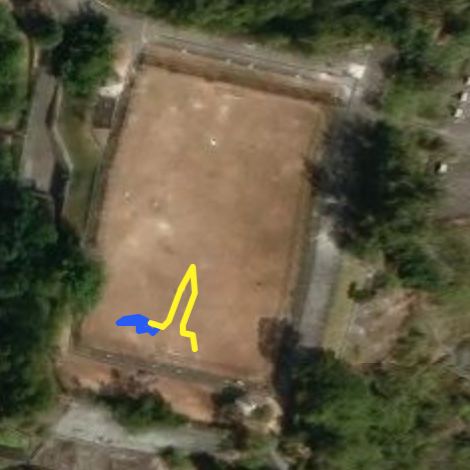
\includegraphics[width=\linewidth]{Included_Images/HomantinMountainTrack.png}\\ 
    \hline
    (b) & 2025 Oct. 12 & Tai Hang Tun & Autonomous flight; UAV hovers over a
    waypoint over bare ground with grass. &
    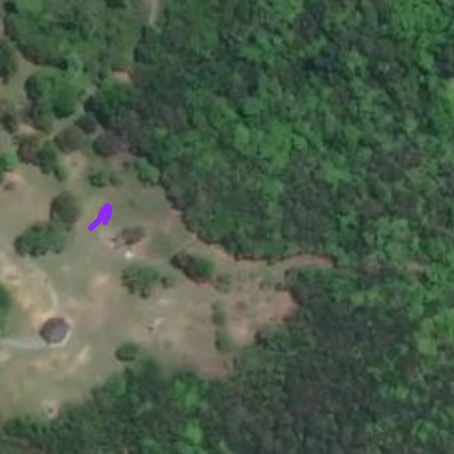
\includegraphics[width=\linewidth]{Included_Images/TaiHangTunGrass.png}\\ 
    \hline
    (c) & 2025 Oct. 12 & Tai Hang Tun & Autonomous flight; UAV hovers over a
    waypoint over dense vegetation. &
    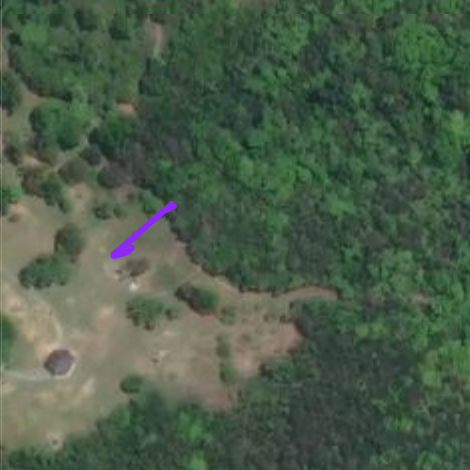
\includegraphics[width=\linewidth]{Included_Images/TaiHangTunTree.png}\\ 
    \hline
    (d) & 2025 Oct. 12 & Tai Hang Tun & Manual flight with dynamic trajectory
    over both bare ground and vegetation. &
    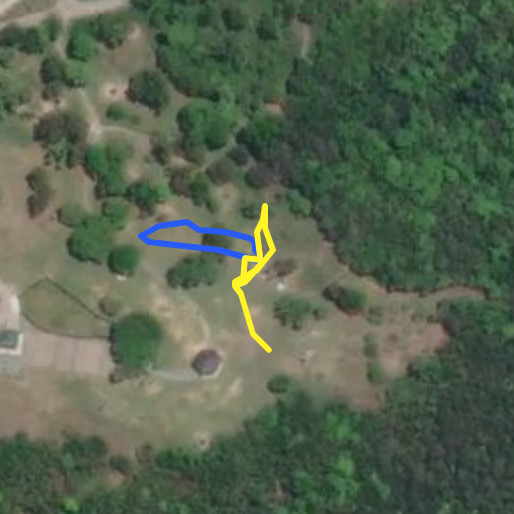
\includegraphics[width=\linewidth]{Included_Images/TaiHangTunDynamic.png}\\ 
    \hline
    (e) & 2025 Nov. 09 & Nam Sang Wai & Autonomous flight; UAV hovers over a
    waypoint over bare soil. &
    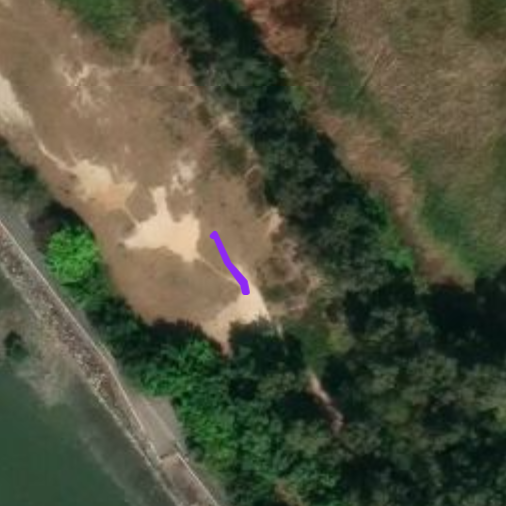
\includegraphics[width=\linewidth]{Included_Images/NamSangWai094324.png}\\ 
    \hline
    (f) & 2025 Nov. 09 & Nam Sang Wai & Autonomous flight; UAV hovers over a
    waypoint over dense vegetation. &
    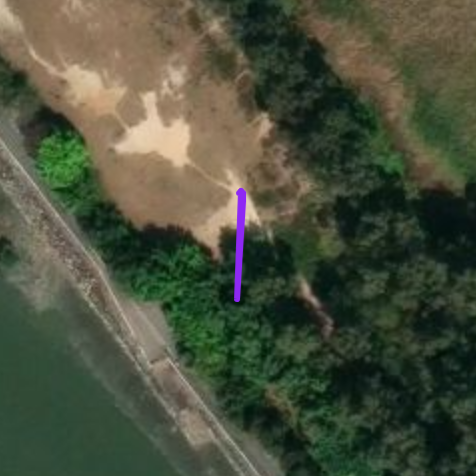
\includegraphics[width=\linewidth]{Included_Images/NamSangWai101211.png}\\ 
    \hline
    (g) & 2025 Nov. 09 & Nam Sang Wai & Autonomous flight; UAV hovers multiple
    waypoints over dense vegetation. &
    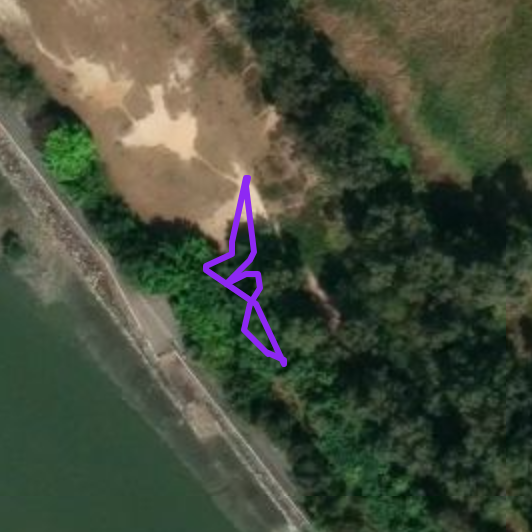
\includegraphics[width=\linewidth]{Included_Images/NamSangWai103755.png}\\    
    \hline
    (h) & 2025 Nov. 09 & Nam Sang Wai & Autonomous flight; UAV flies over a
    survey area that covers dense vegetation. &
    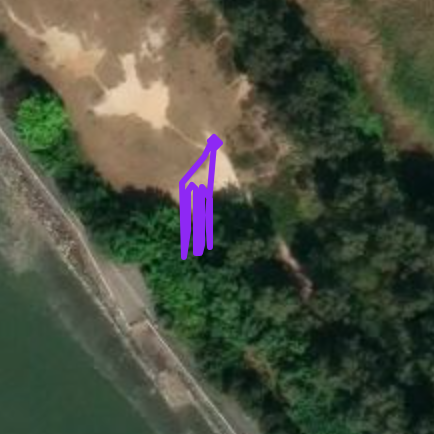
\includegraphics[width=\linewidth]{Included_Images/NamSangWai113425.png}\\ 
    \hline
    (i) & 2025 Nov. 09 & Nam Sang Wai & Autonomous flight; UAV flies over a
    survey area that covers dense vegetation. &
    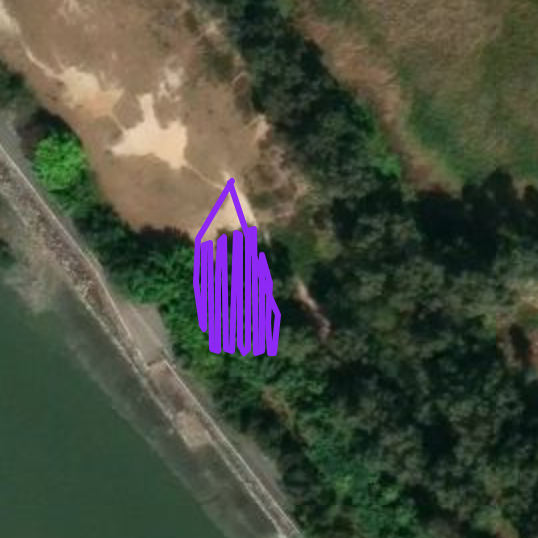
\includegraphics[width=\linewidth]{Included_Images/NamSangWai113830.png}\\ 
    \hline
    (j) & 2025 Nov. 09 & Nam Sang Wai & Autonomous flight; UAV flies over a
    survey area that covers dense vegetation. &
    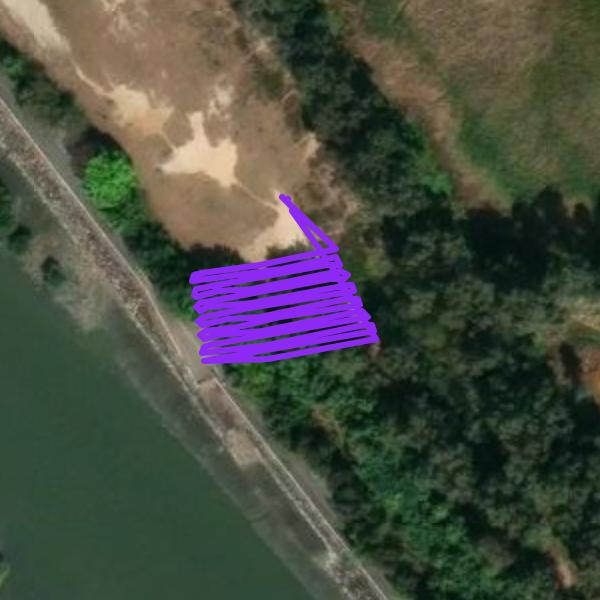
\includegraphics[width=\linewidth]{Included_Images/NamSangWai115109.png}\\ 
    \hline
    (k) & 2026 Feb. 01 & Mount Davis & Autonomous flight; UAV flies over a
    survey area that covers bare ground with grass. &
    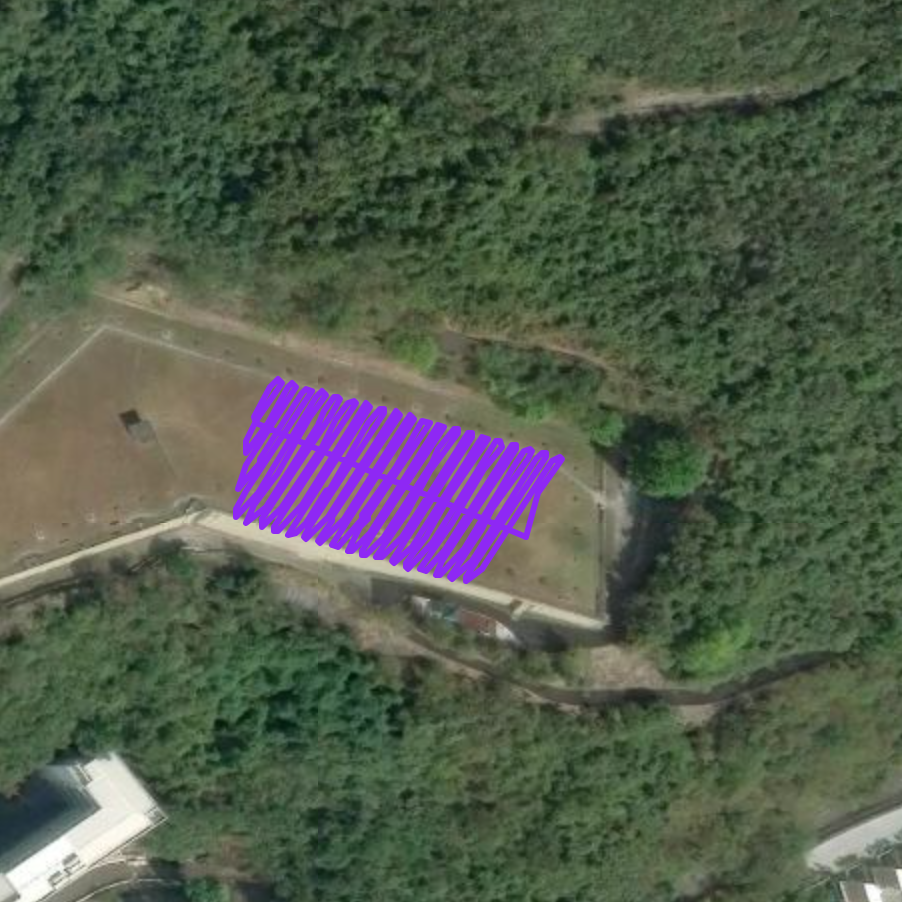
\includegraphics[width=\linewidth]{Included_Images/MtDavis1_1.png}\\
    \hline
    (l) & 2026 Feb. 01 & Mount Davis & Autonomous flight; UAV flies over a
    survey area that covers dense vegetation. &
    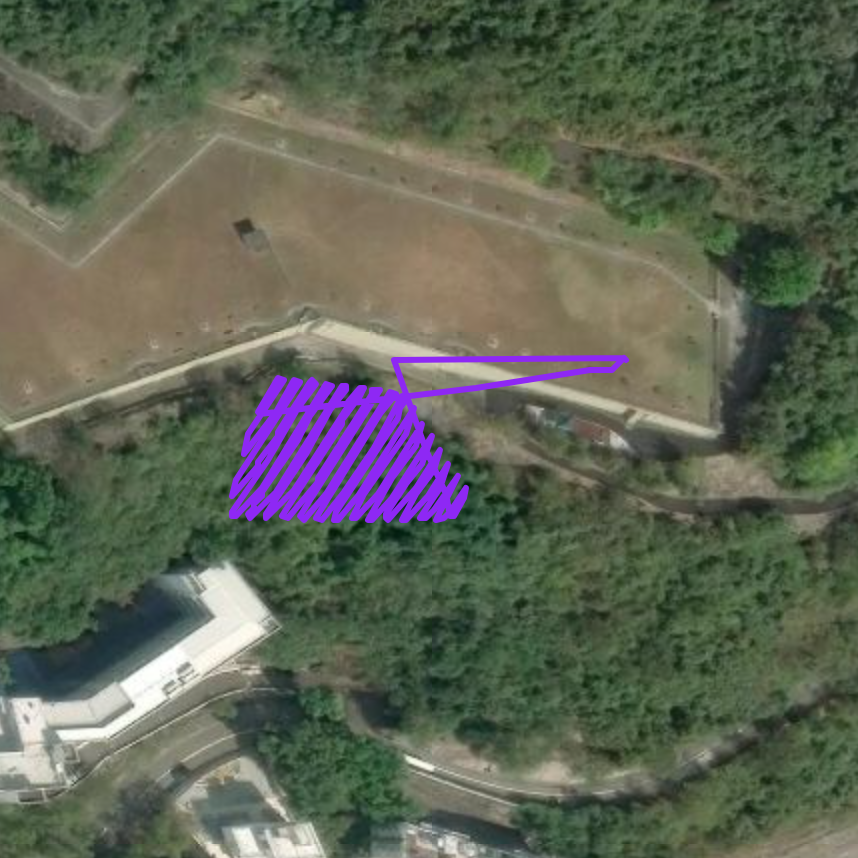
\includegraphics[width=\linewidth]{Included_Images/MtDavis1_2.png}\\
    \hline
    (m) & 2026 Feb. 01 & Mount Davis & Autonomous flight; UAV flies over a
    survey area that covers dense vegetation. &
    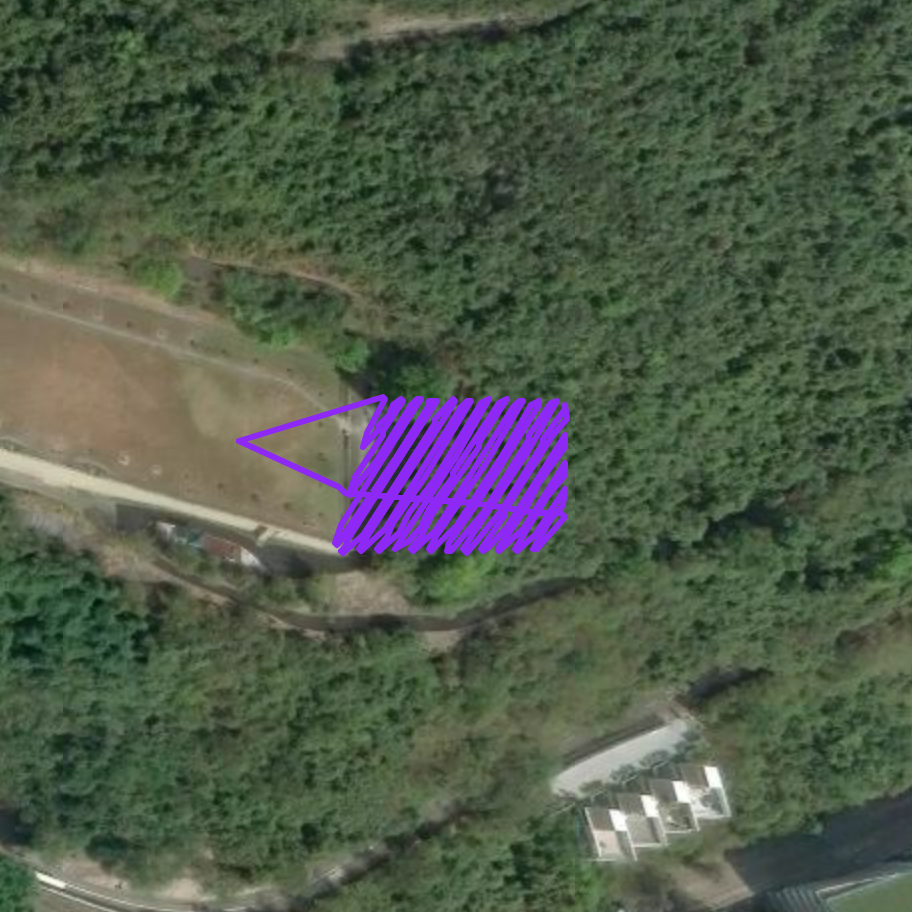
\includegraphics[width=\linewidth]{Included_Images/MtDavis1_3.png}\\
    \hline
    (n) & 2026 Feb. 01 & Mount Davis & Autonomous flight; UAV flies over a
    survey area that covers dense vegetation. &
    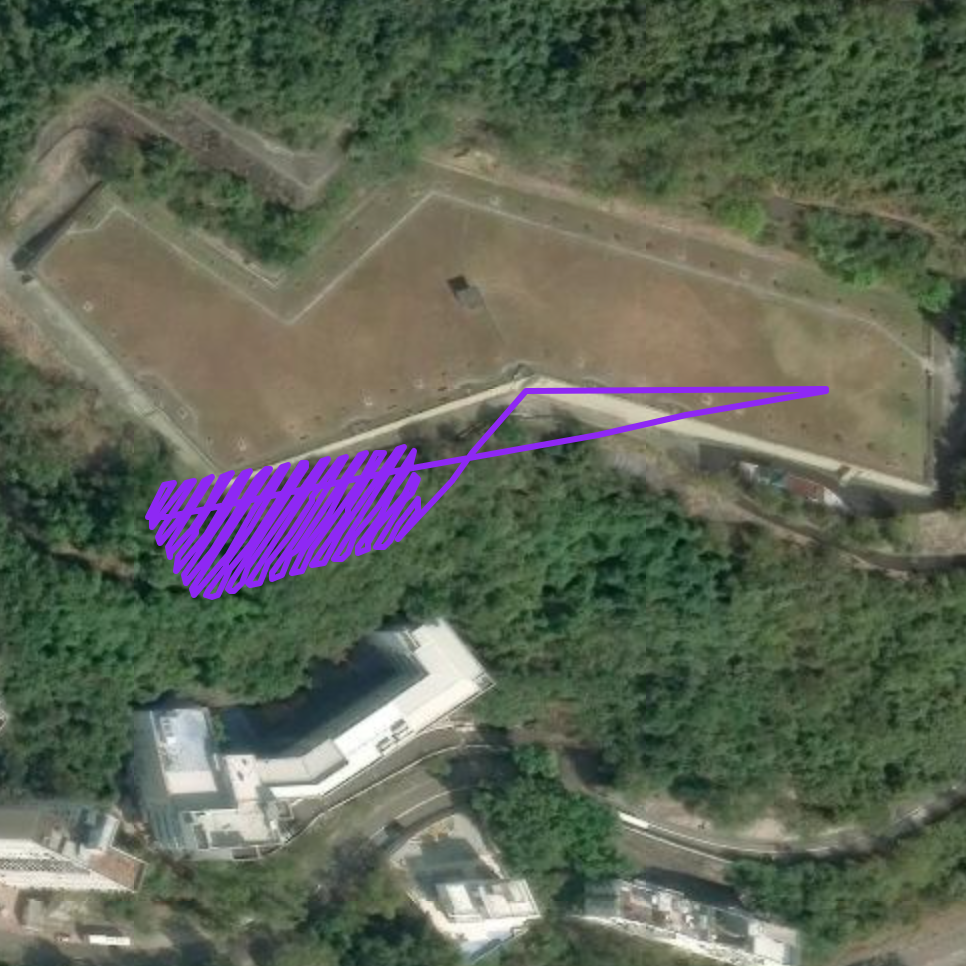
\includegraphics[width=\linewidth]{Included_Images/MtDavis1_4.png}\\
    \hline
    (o) & 2026 Feb. 01 & Mount Davis & Autonomous flight; UAV flies over a
    survey area that covers dense vegetation. &
    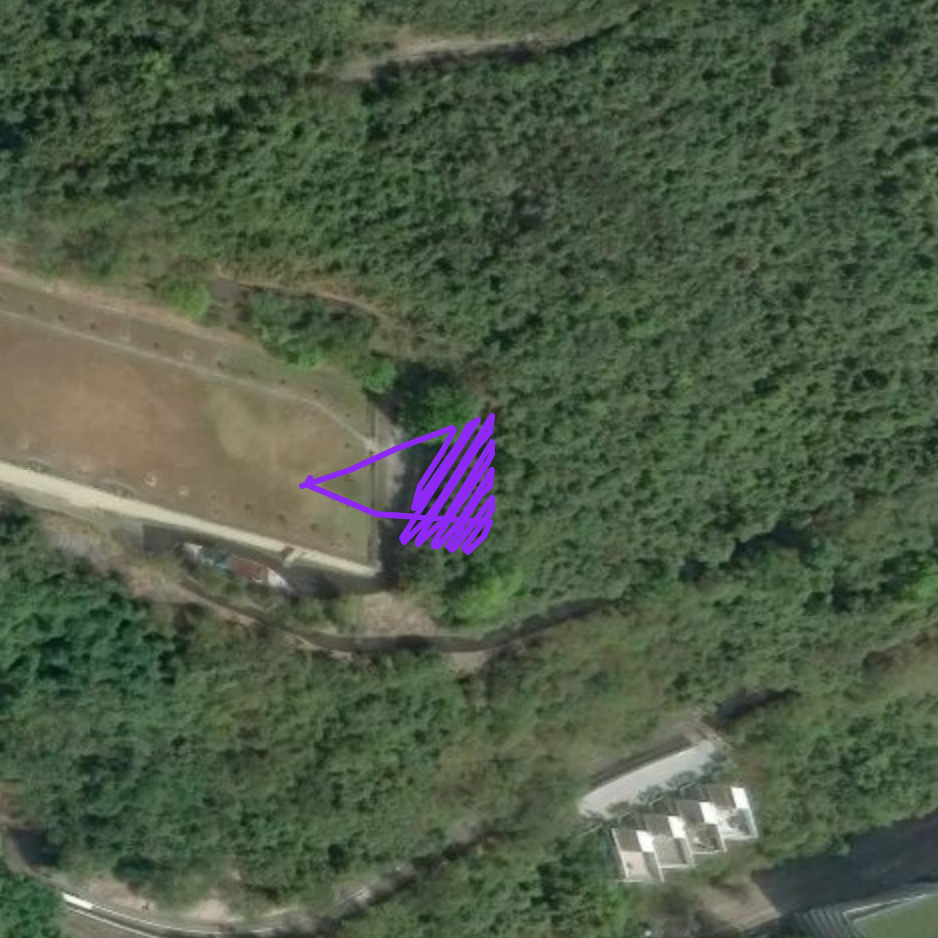
\includegraphics[width=\linewidth]{Included_Images/MtDavis1_5.png}\\
    \hline
    (p) & 2026 Mar. 08 & Shing Mun & Autonomous flight; UAV flies over a survey
    area that covers dense vegetation. &
    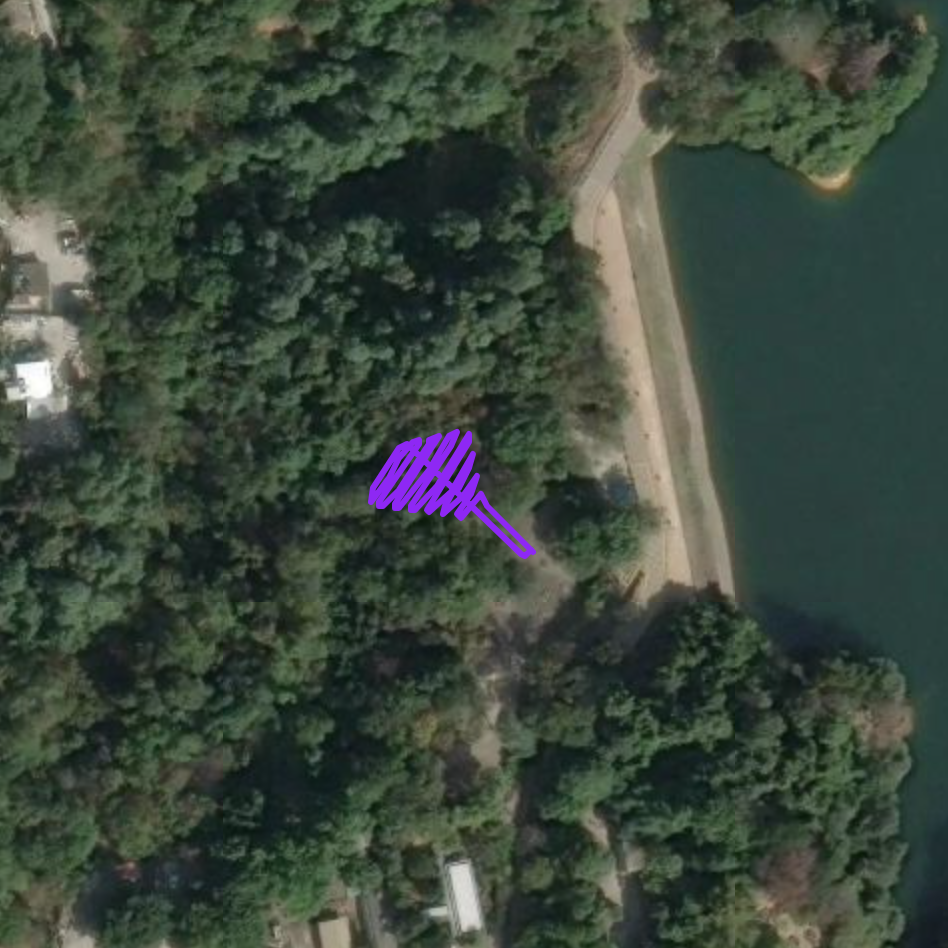
\includegraphics[width=\linewidth]{Included_Images/Shingmun1.png}\\
    \hline
    (q) & 2026 Mar. 08 & Shing Mun & Autonomous flight; UAV flies over a survey
    area that covers dense vegetation. &
    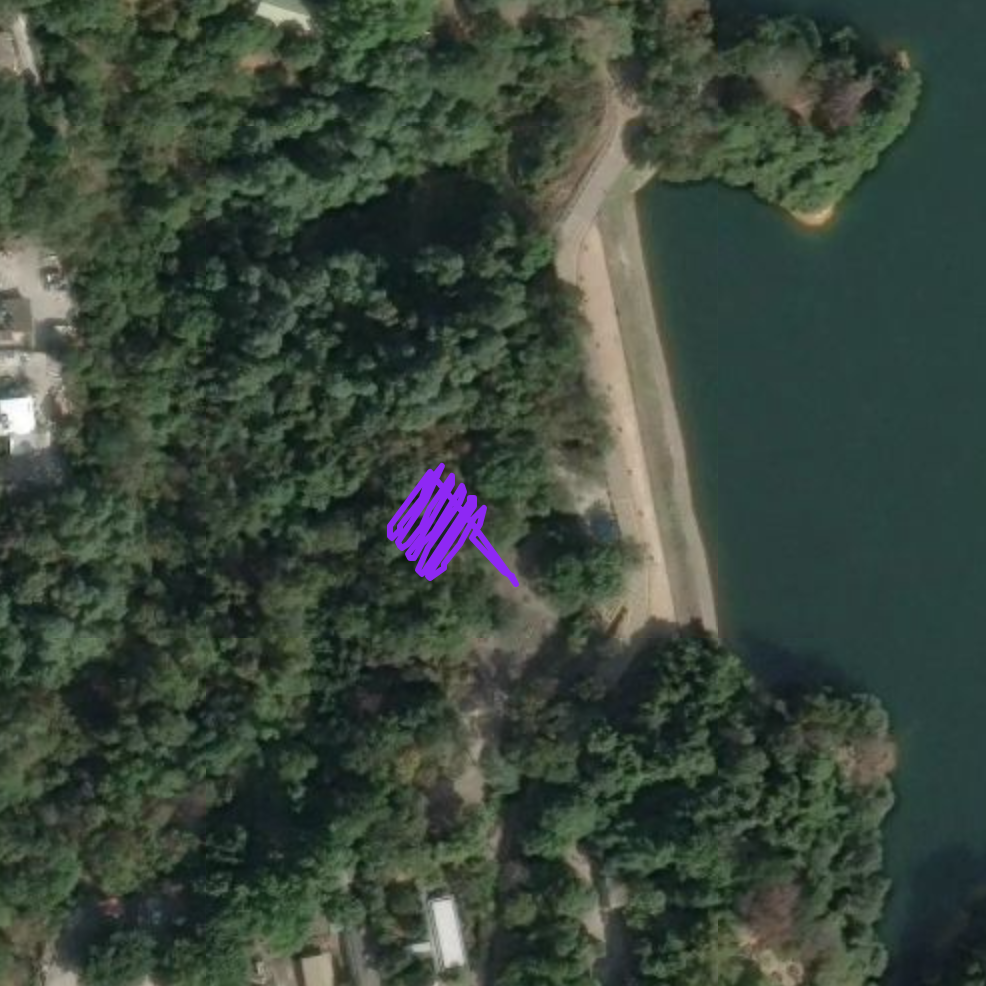
\includegraphics[width=\linewidth]{Included_Images/Shingmun2.png}\\
    \hline
    (r) & 2026 Mar. 08 & Shing Mun & Autonomous flight; UAV flies over a survey
    area that covers dense vegetation. &
    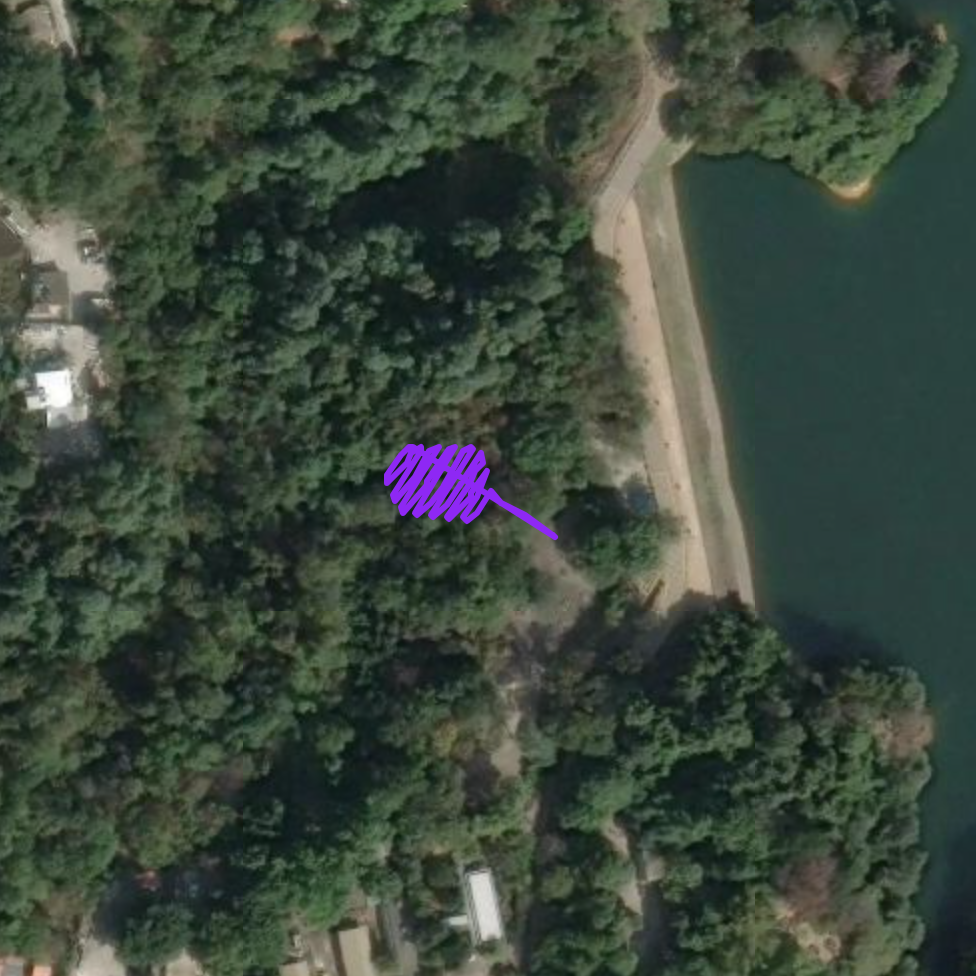
\includegraphics[width=\linewidth]{Included_Images/Shingmun3.png}\\
    \hline
    (s) & 2026 Mar. 08 & Shing Mun & Autonomous flight; UAV flies over a survey
    area that covers dense vegetation. &
    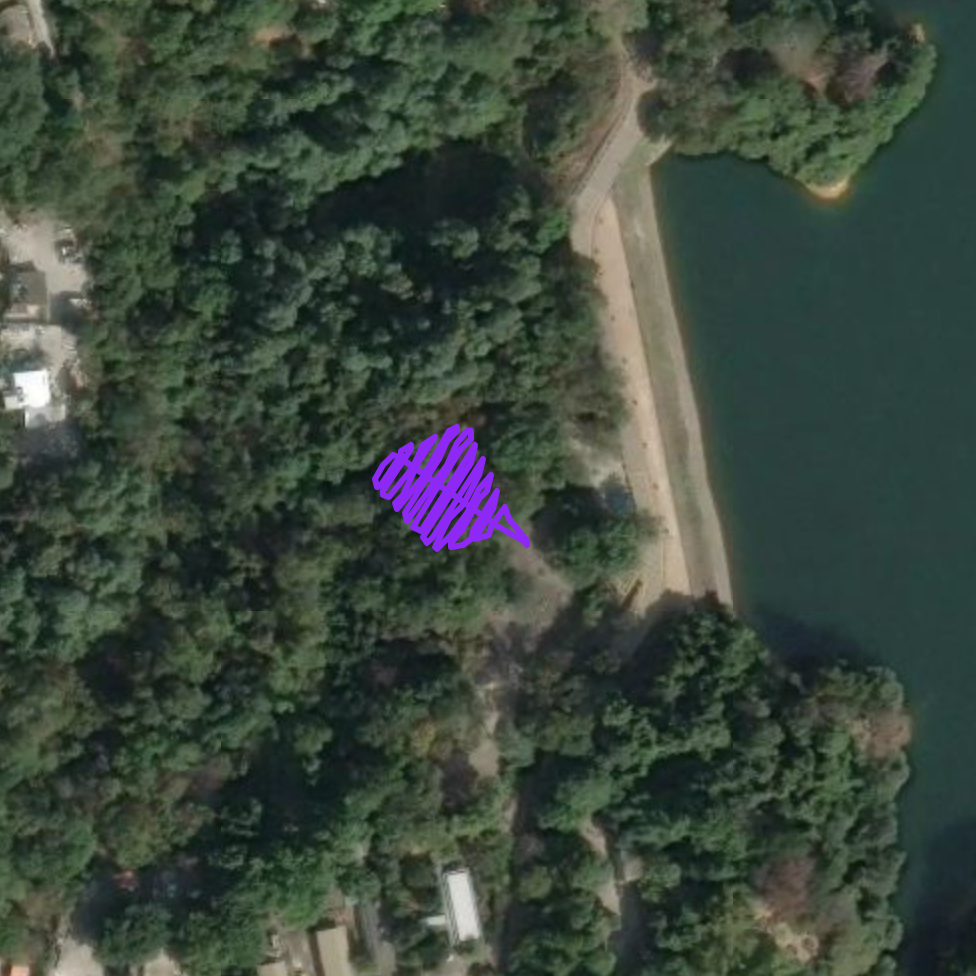
\includegraphics[width=\linewidth]{Included_Images/Shingmun4.png}\\
    \hline
    (t) & 2026 Mar. 08 & Shing Mun & Autonomous flight; UAV hovers over 2
    different waypoints over dense vegetation. &
    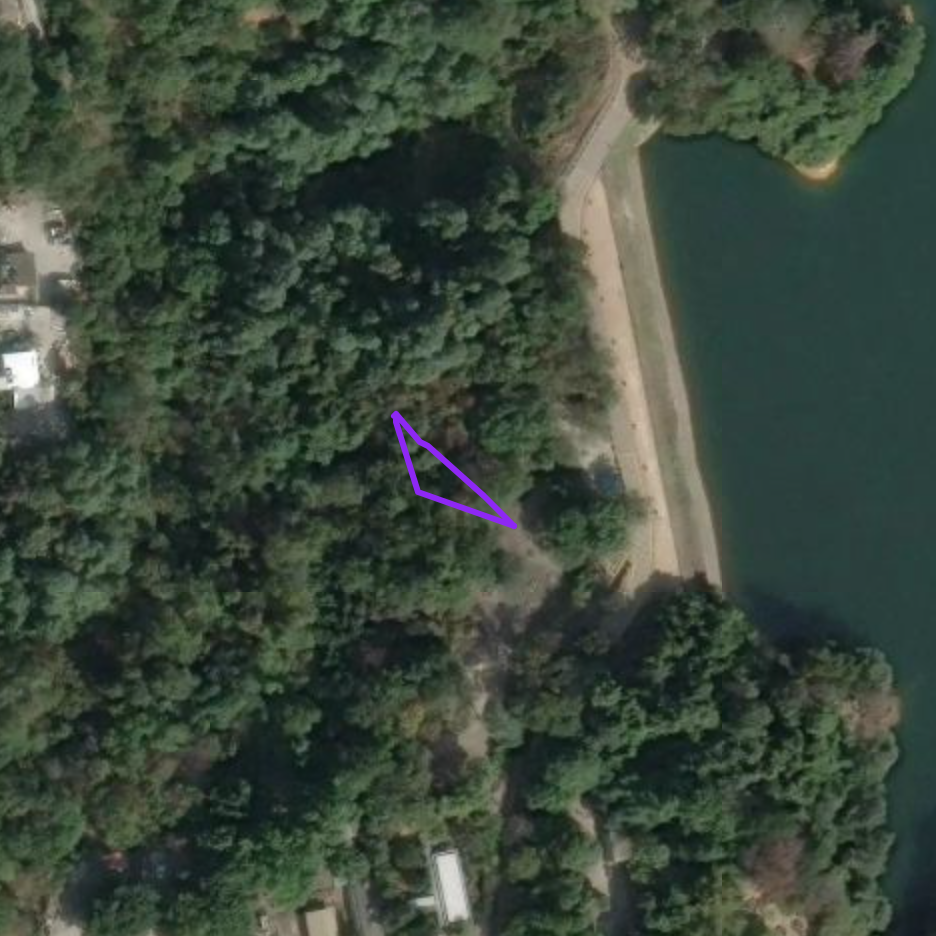
\includegraphics[width=\linewidth]{Included_Images/Shingmun5.png}\\
    \hline
    (u) & 2026 Mar. 31 & Mount Davis & Autonomous flight; UAV flies over a
    survey area that covers bare ground with grass. &
    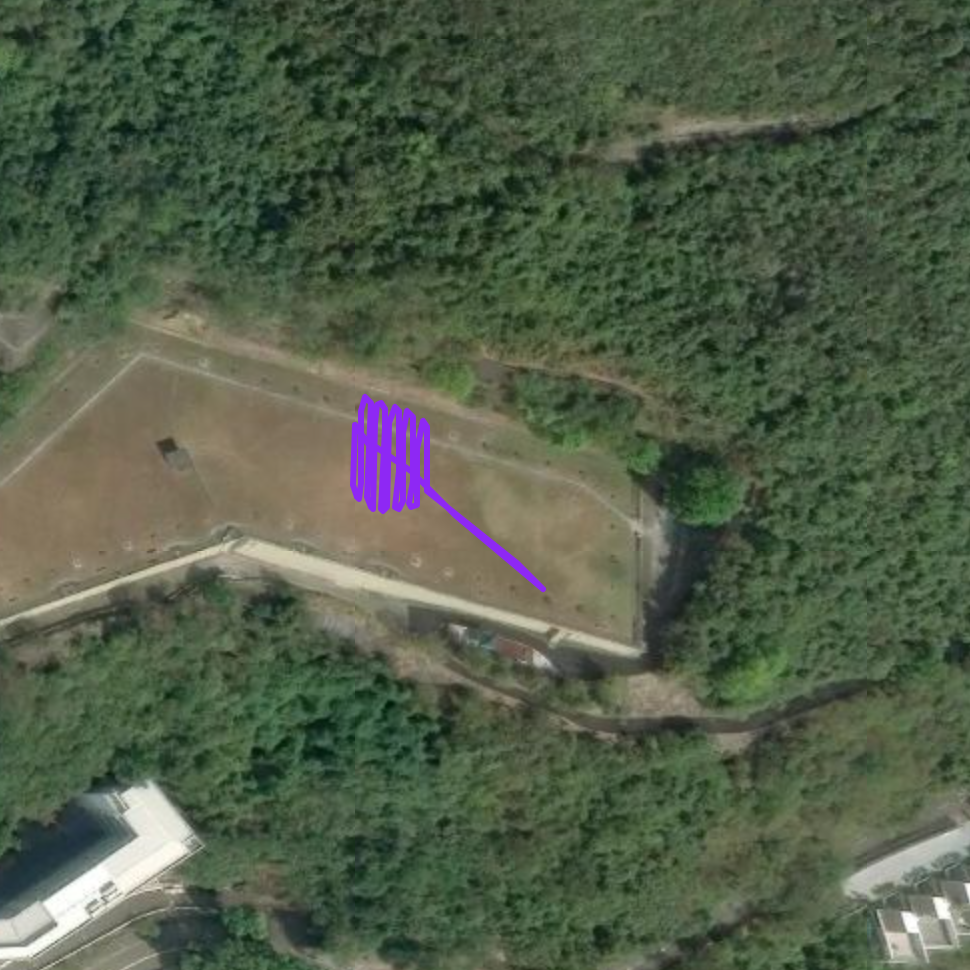
\includegraphics[width=\linewidth]{Included_Images/MtDavis2_1.png}\\
    \hline
    (v) & 2026 Mar. 31 & Mount Davis & Autonomous flight; UAV flies over a
    survey area that covers bare ground with grass. &
    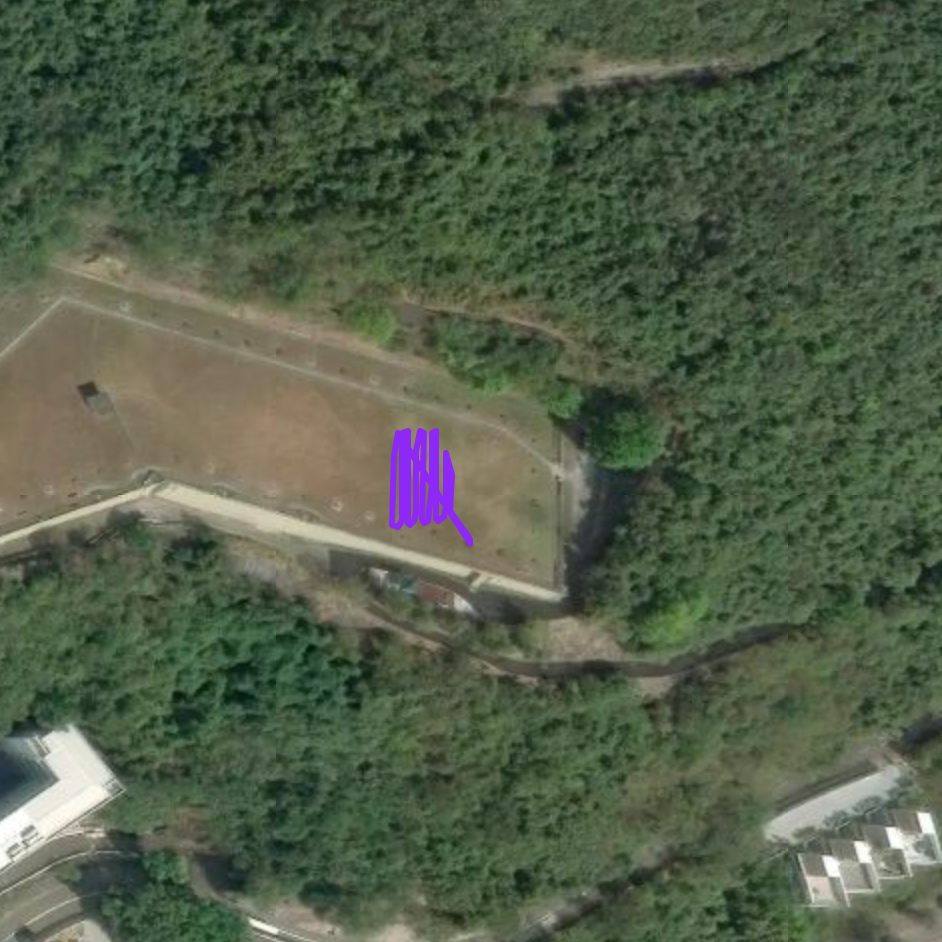
\includegraphics[width=\linewidth]{Included_Images/MtDavis2_2.png}\\
    \hline
    (w) & 2026 Mar. 31 & Mount Davis & Autonomous flight; UAV flies over a
    survey area that covers dense vegetation. &
    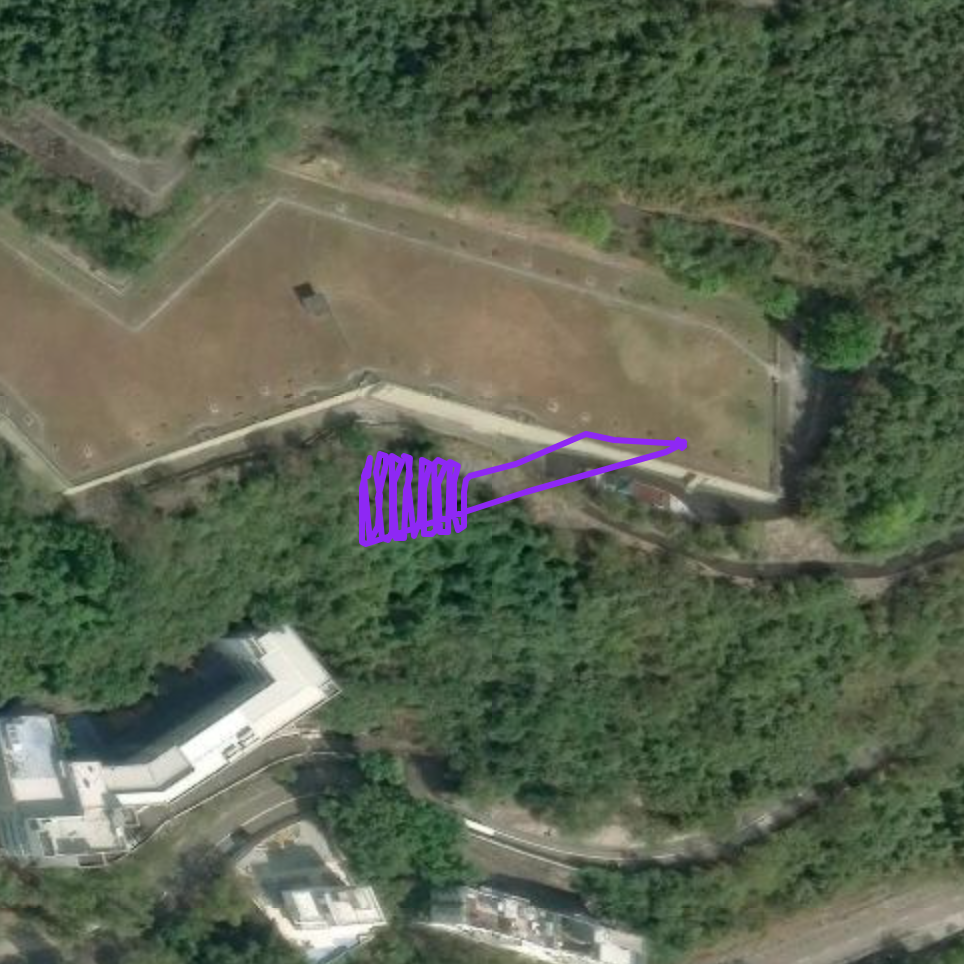
\includegraphics[width=\linewidth]{Included_Images/MtDavis2_3.png}\\
    \hline
    (x) & 2026 Mar. 31 & Mount Davis & Autonomous flight; UAV flies over a
    survey area that covers dense vegetation. &
    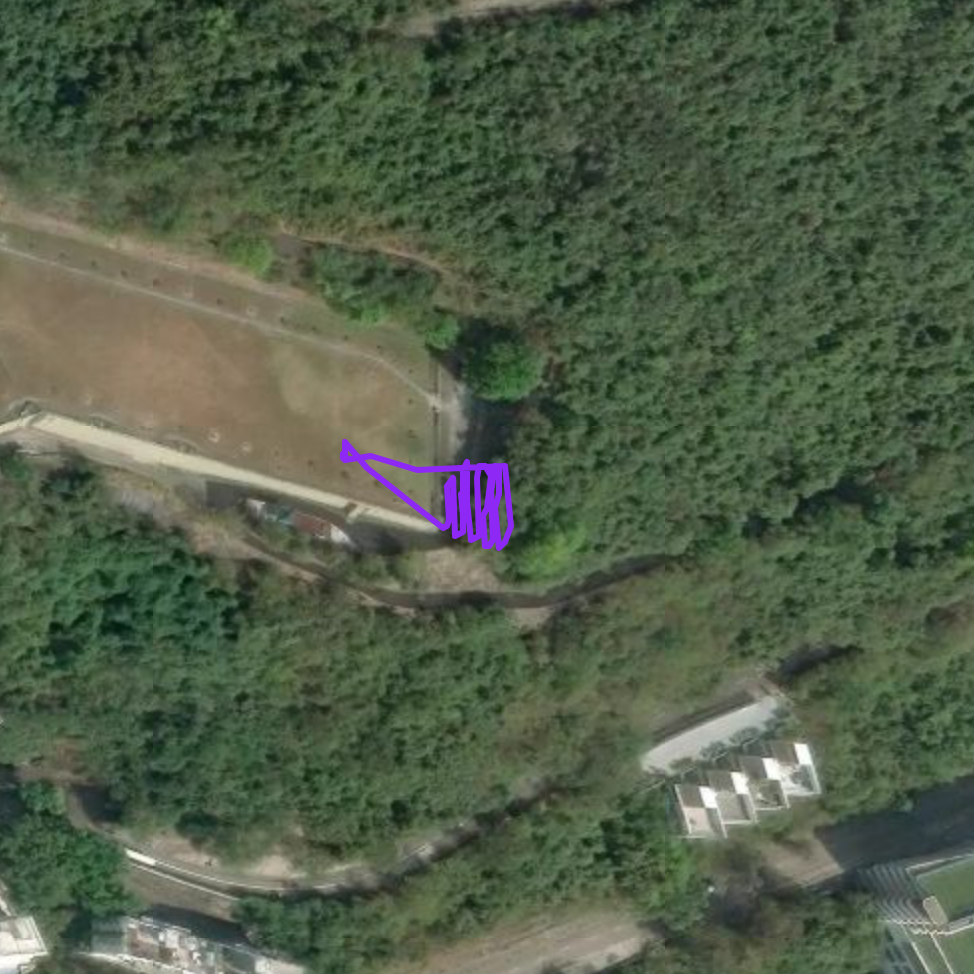
\includegraphics[width=\linewidth]{Included_Images/MtDavis2_4.png}\\
    \hline
\end{tabularx} 


% --- Case Study ---
\newpage
\section{Case Study}
In this case study, the results of the experiment conducted at Mount Davis on
March 31, 2026, are discussed to demonstrate the final integrated system. A
total of four flights were executed (flights (u) - (x) in Table
\ref{Experiment-Summary}) to collect feature-extensive LiDAR and GNSS-R datasets
in an environment that contains both dense vegetation and ground with sparse
vegetation (grass).

\subsubsection{Path Planning and Execution}
In this experiment, the trajectory is planned to ascend and maintain at an
altitude of 35 meters during the survey mission. The paths in the survey area
are spaced at 2 meter intervals, with the turnaround buffer distance set at 5
meter. Figure \ref{fig:planned_path} shows real time flight path execution on
the QGround Control as well as in the real-world environment.
\begin{figure}[H]
    \centering
    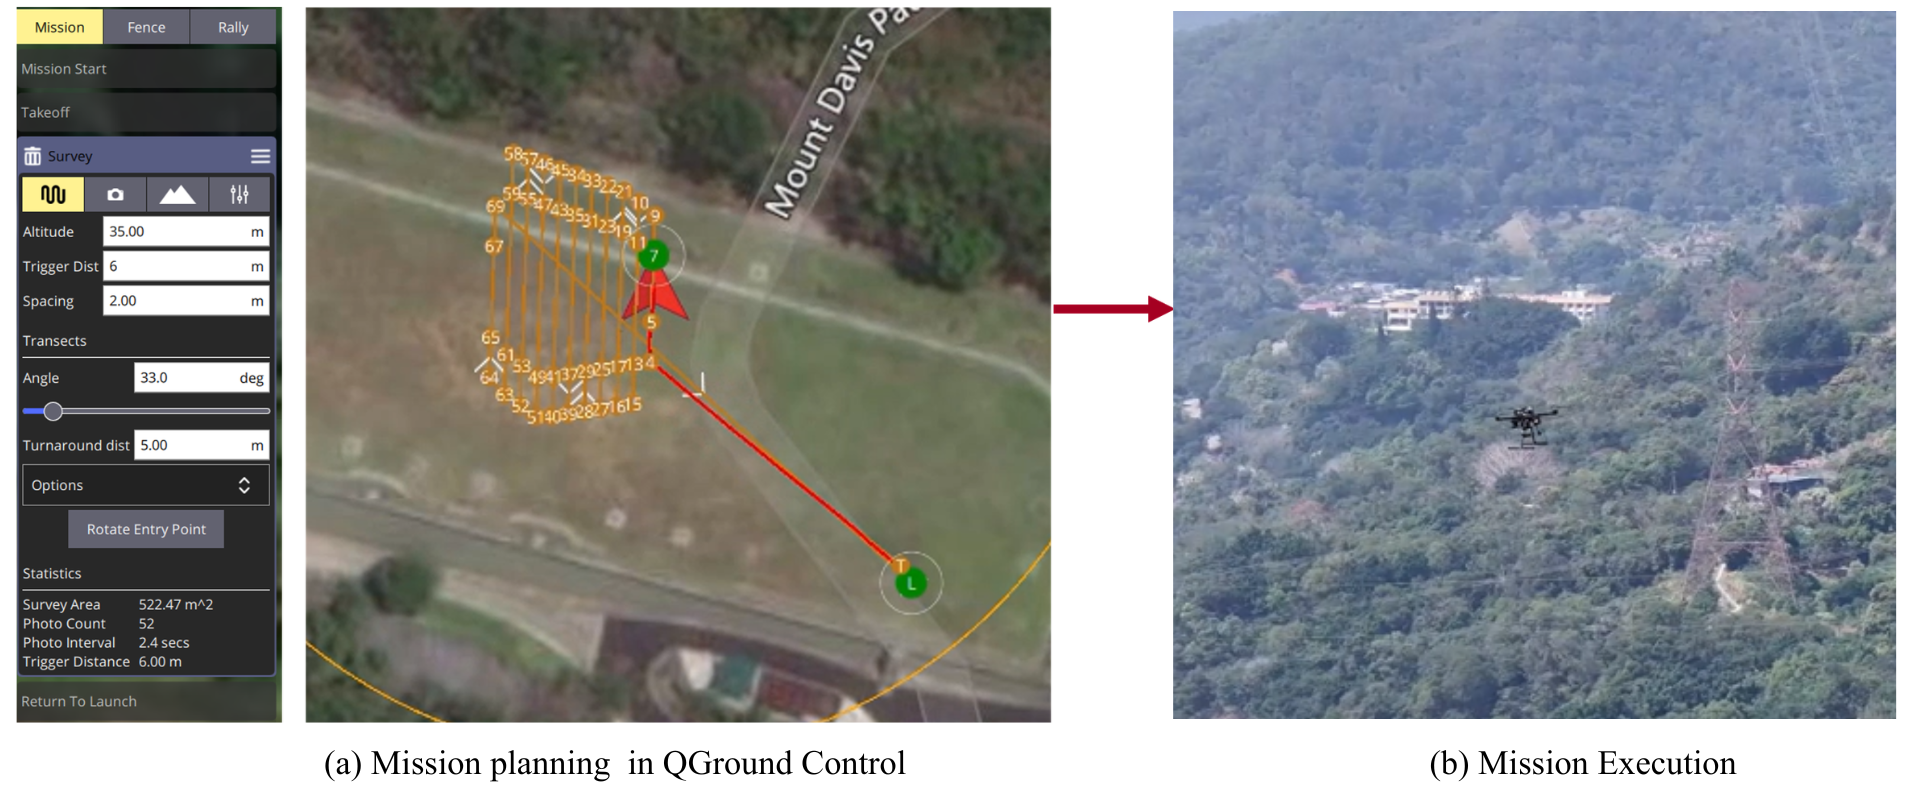
\includegraphics[width=1.0\textwidth]{Included_Images/KeyExperiment_Plannedpath.png}
    \caption{Mission Planning and Execution Results}
    \label{fig:planned_path}
\end{figure}

\subsubsection{LiDAR SLAM}
For this dataset, LiDAR point clouds were processed using two techniques: the standard Fast-LIO odometry and PGO with GPS fusion (PGO+GPS). As shown in the figures below, both Fast-LIO and (PGO+GPS) is able to showcase point clouds of different features such as bare ground and tree canopies. In this case, the vegetation map generated can be used as a geometric reference for GNSS-R signals. In PGO+GPS, the green trajectory indicates the LiDAR odometry, and the 3-axis trajectory indicates the GPS trajectory. 
\begin{figure}[H]
    \centering
    \begin{subfigure}{0.6\textwidth}
        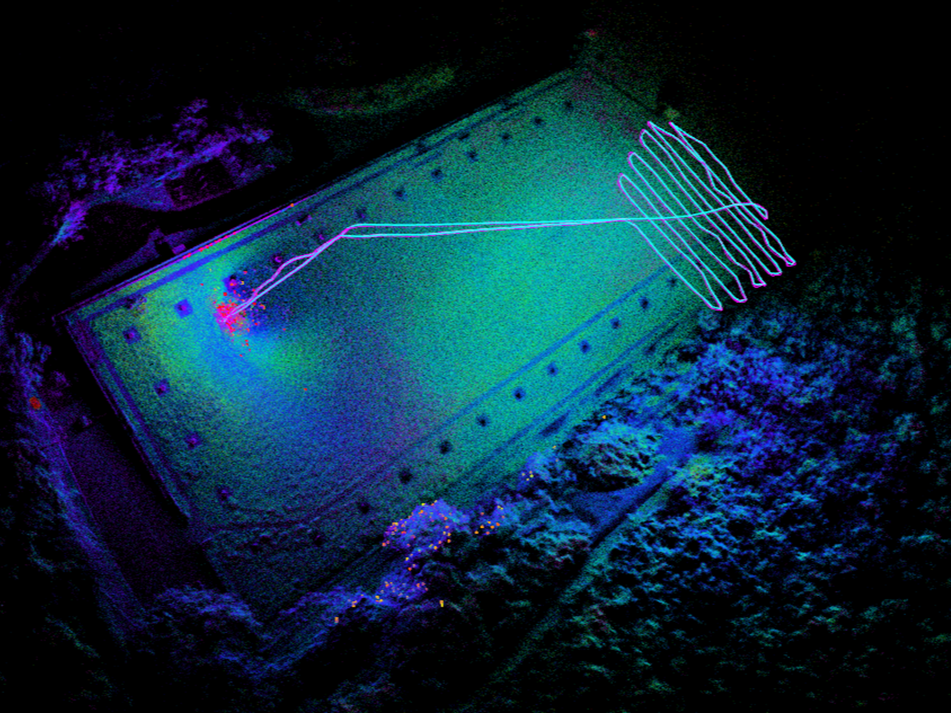
\includegraphics[width=\textwidth]{Included_Images/case_FL.png}
        \caption{Fast-LIO}
    \end{subfigure}
    
    \par\medskip
    
    \begin{subfigure}{0.6\textwidth}
        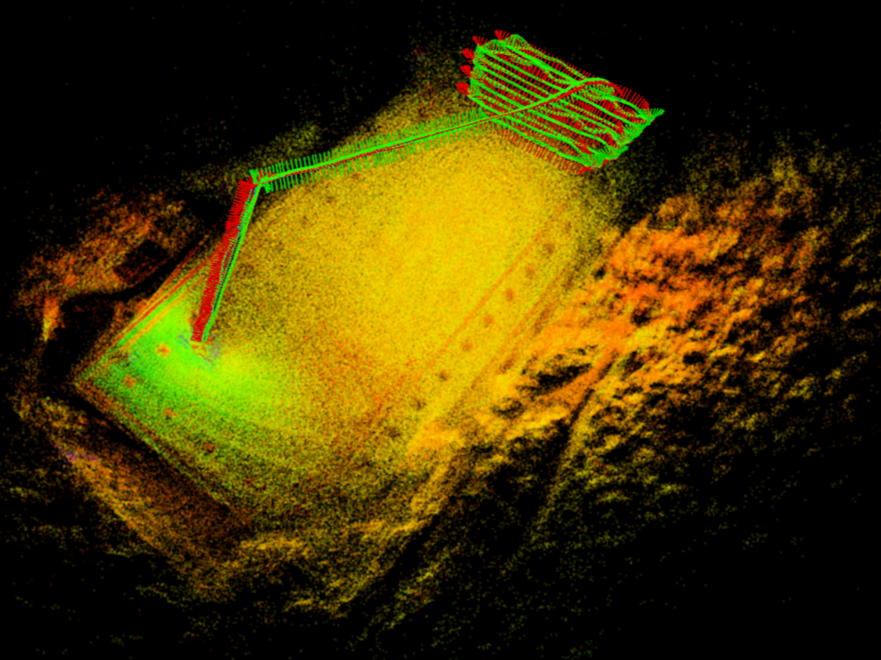
\includegraphics[width=\textwidth]{Included_Images/case_pgo.png}
        \caption{PGO+GPS}
    \end{subfigure}
    \caption{LiDAR SLAM results using two different techniques.}
\end{figure}

\subsubsection{GNSS-R Analysis and Modelling}
After the successful collection of GNSS data during the flight missions, GNSS
measurements are extracted during post-processing to calculate the $C/N_0$ ratio
and the excess pseudorange delay. Then, the FFZ of each reflected GNSS signal is
calculated and plotted onto a satellite image map, where the colors of Figure
\ref{CNR and Delay Case Study}(a) indicate the $C/N_0$ ratio between the
reflected signal and the direct signal, while the colors of Figure \ref{CNR and
Delay Case Study}(b) indicate the excess pseudorange delay of the reflected
signals. 
\begin{figure}[H]
    \centering
    \begin{subfigure}{0.7\textwidth}
        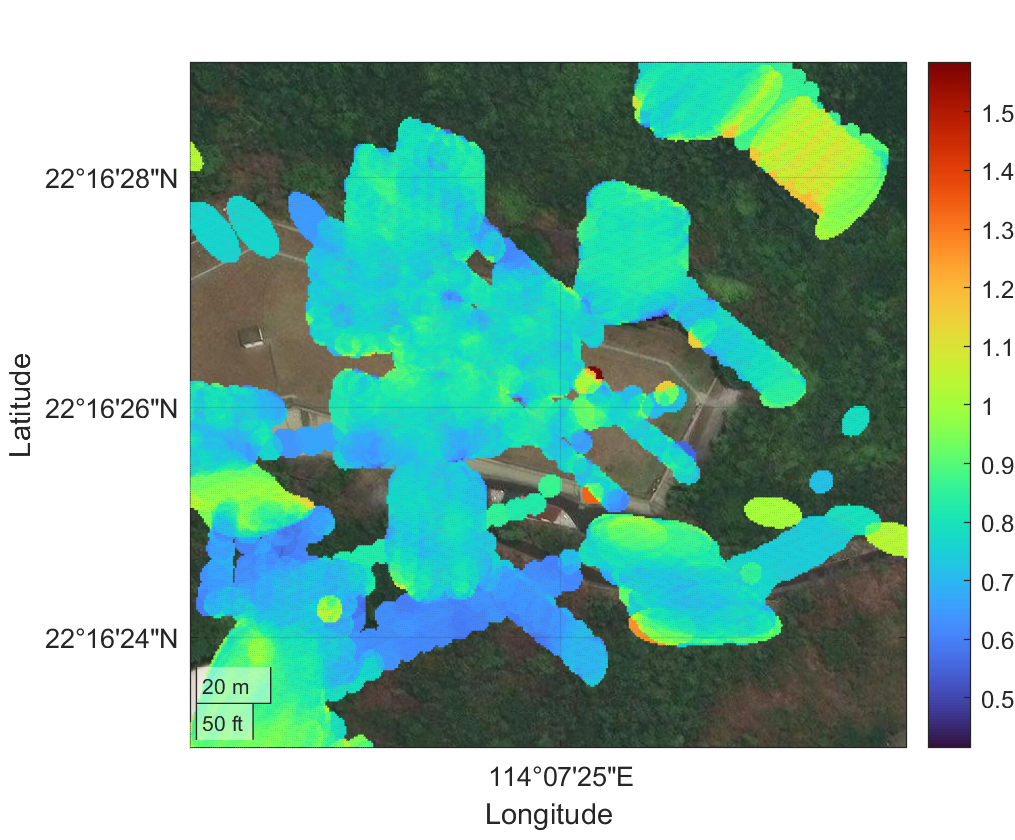
\includegraphics[width=\textwidth]{Included_Images/casestudy_CNR.png}
        \caption{$C/N_0$ Ratio Over FFZs}
    \end{subfigure}
    \vfill
    \begin{subfigure}{0.7\textwidth}
        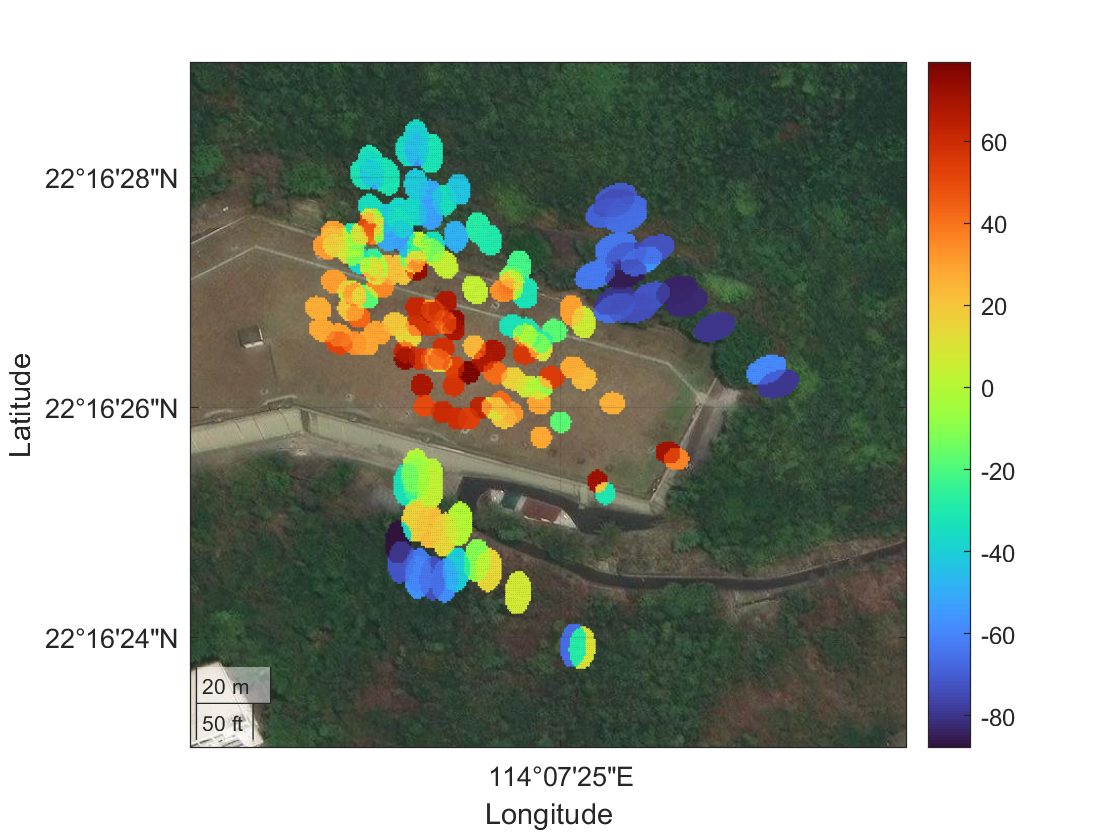
\includegraphics[width=\textwidth]{Included_Images/casestudy_excess_pr_delay.png}
        \caption{Excess Pseudorange Delay Over FFZs}
    \end{subfigure}
    \caption{Received $C/N_0$ ratios and excess pseudorange delays during the case study experiment, plotted over the FFZs of the reflected signals.}
    \label{CNR and Delay Case Study}
\end{figure}
While no clear boundaries are present in the plot of $C/N_0$ ratio since the
difference in $C/N_0$ ratio mainly exists between vegetation and water surfaces,
it is evident that the excess pseudorange delay of the signals reflecting off
ground with grass tends to be greater than the excess pseudorange delay of the
signals reflecting off vegetation. Additionally, given the fact that the excess
pseudorange delay tends to be negative over vegetation, it can be implied that
the signals reflected off the dense canopy rather than propagating through to
reflect off from the ground.
Using the correlations between GNSS measurement parameters and the RGB values of
CIR image pixels that fall within the FFZs (summarized in Section 6.3), the CIR
image colors within each FFZ of this experiment were also reconstructed, as
shown in Figure \ref{Case Study CIR} below. Here, the FFZs over dense canopies
and the FFZs over ground with sparse vegetation could be clearly distinguished,
demonstrating the potential of GNSS as an alternative remote sensing system.
\begin{figure}[H]
    \centering
    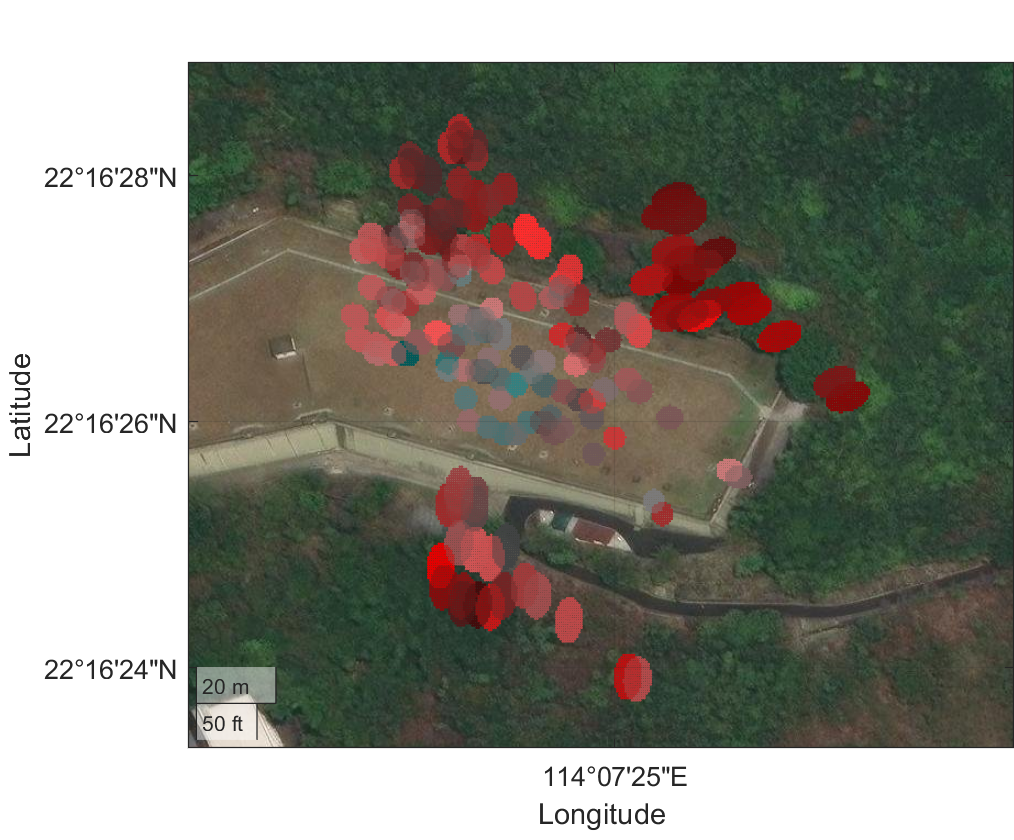
\includegraphics[width=0.8\textwidth]{Included_Images/casestudy_CIR.png}
    \caption{Reconstructed CIR image color using GNSS measurements, plotted over the FFZs of the reflected signals.}
    \label{Case Study CIR}
\end{figure}
\subsubsection{Machine Learning Signal Classification and Vegetation Boundary Detection}
Figure below shows the FFZ centroids for all the satellites tracked during the experiment. The spatial distribution
of the predictions align well with the visible terrain on the map. For example, satellite E21, E34 are classified as tree reflected
while their centroids also fall over the vegetated area predominantly.

The per satellite confidence plots are also shown below. The show that the classifier performs
well overall with mean confidence ranging from 0.77 to 0.99. Lower confidence satellites are also observed (E27, E30). However, their
FFZs fall near the boundary transition zones which explains the ambiguity.
\begin{figure}[H]
    \centering
    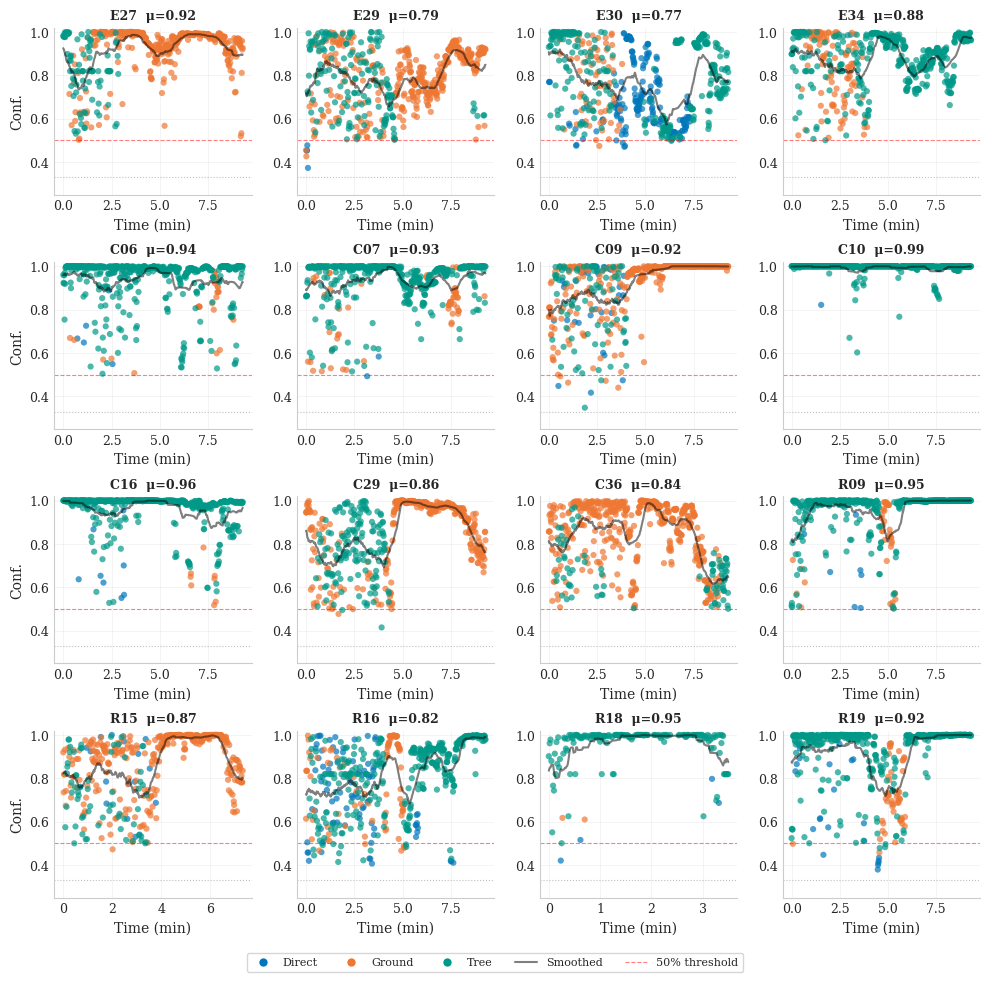
\includegraphics[width=0.75\textwidth]{Included_Images/mtdavis_confidence.png}
    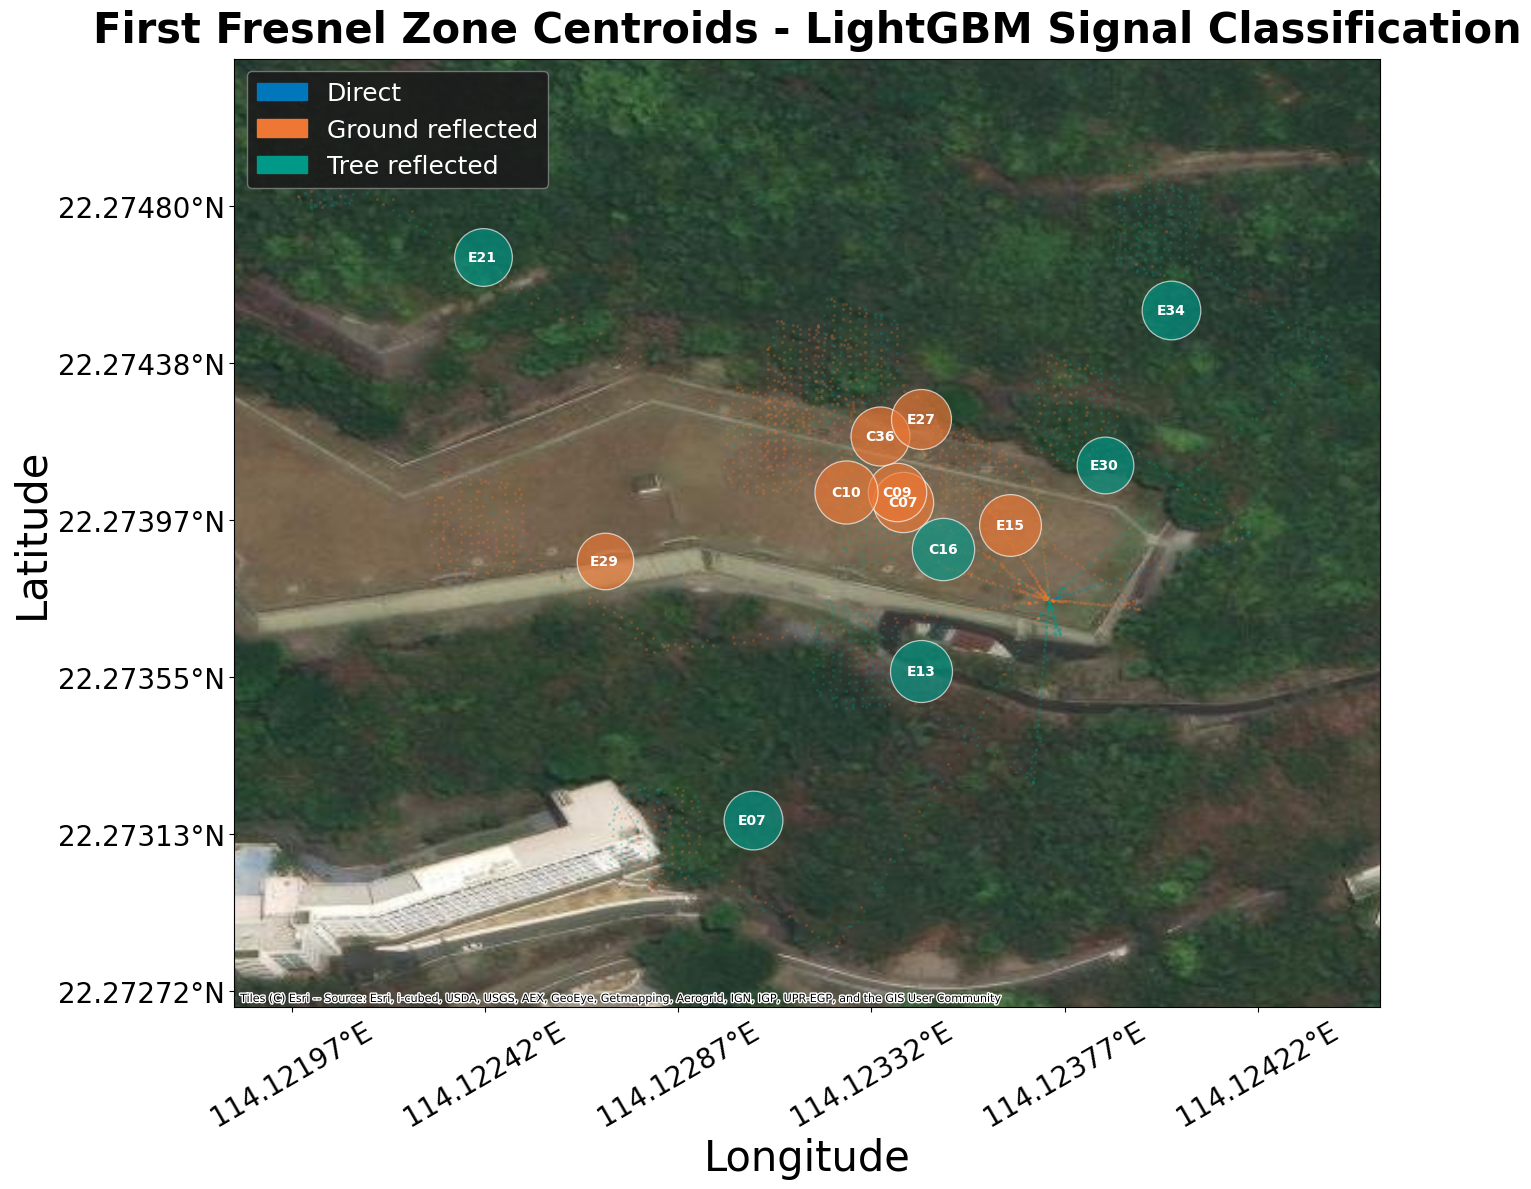
\includegraphics[width=0.75\textwidth]{Included_Images/mtdavis_ffzcon.png}
    \caption{Confidence and FFZ centroid plotting for the experiment.}
\end{figure}
The classification results from the ML pipeline was further validated by the GNSS-R results. The figure below shows the
comparison. The classification results clearly align with the results from the GNSS-R pipeline meaning that the prediction
results are trustworthy and can be used to remove any noise from the dataset for better processing of the GNSS-R pipeline.
 \begin{figure}[H]
    \centering
    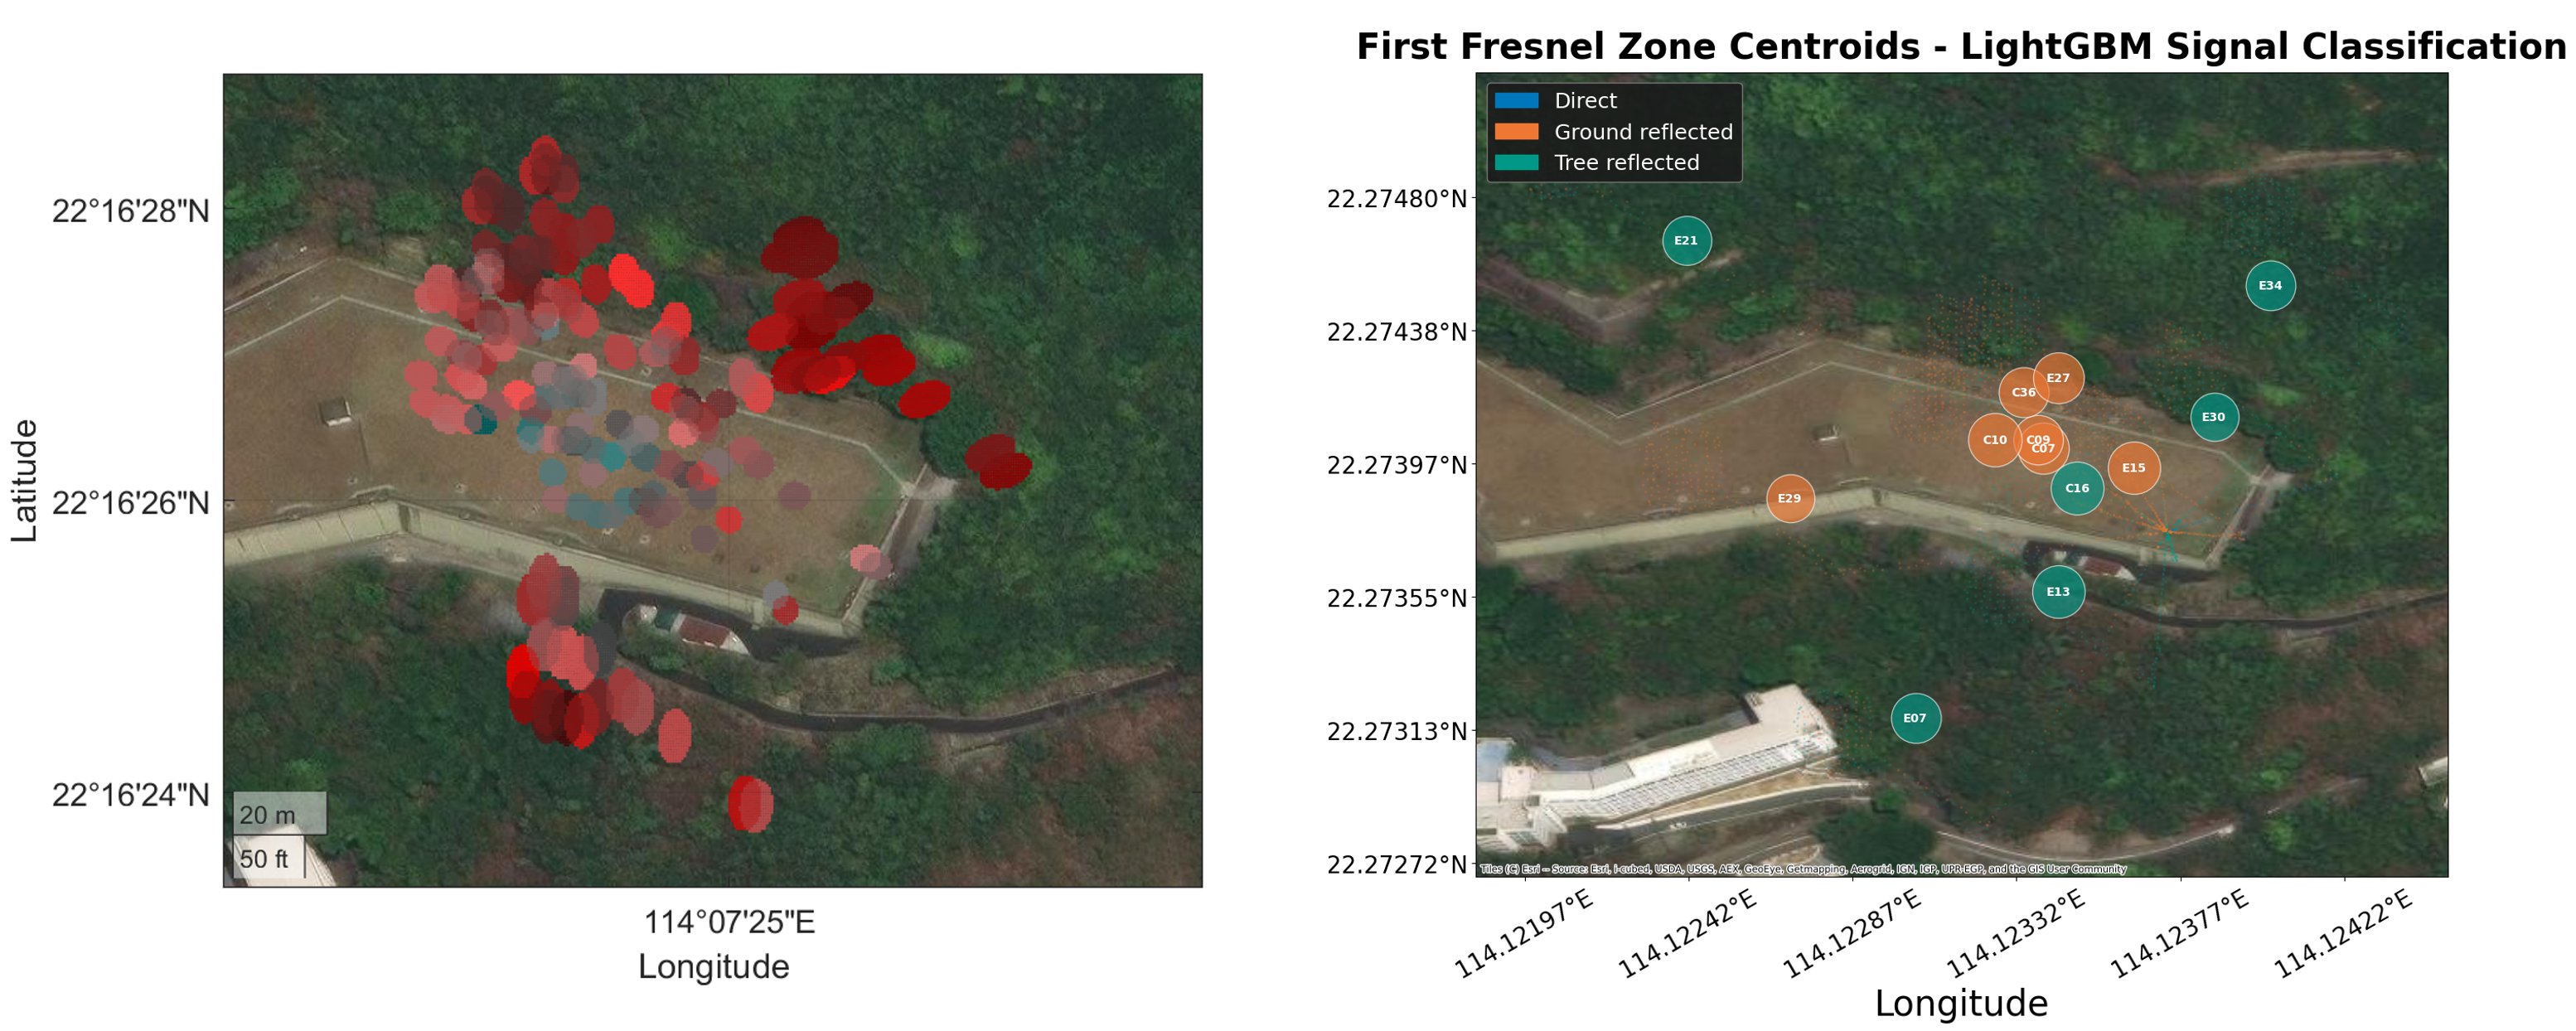
\includegraphics[width=0.8\textwidth]{Included_Images/ML-FFZ.png}
    \caption{Comparison between ML classification results and GNSS-R results.}
\end{figure}


% --- Conclusion ---
\section{Conclusion}
In conclusion, this project successfully established a comprehensive UAV-based
framework for remote sensing, which integrates autonomous path planning for
optimized vegetation coverage, LiDAR SLAM for accurate canopy mapping, GNSS-R
for ground feature sensing, and machine learning for vegetation detection. 

The path planning framework leverages both waypoint-based navigation and
coverage path planning to enable autonomous UAV navigation for efficient
vegetation sensing. First, the satellite images of the mission location are
processed to obtain greenery regions for survey missions. The interactive path
planner system developed within this pipeline will then identify the optimal
detection area through clustering the potential First Fresnel Zones of
reflection, such that a suitable sweeping distance for coverage path planning
can be derived. Ultimately, an optimized survey mission can be planned and
executed through QGroundControl, which enables the collection of LiDAR and GNSS
data.

The LiDAR data collected during the flight missions is used to generate 3D
canopy maps within a point cloud environment. This is achieved through an
initial time synchronization between the LiDAR sensor data and the Pixhawk
internal clock. Afterward, LiDAR odometry is applied in the front end while pose
graph optimization SLAM is applied in the back end. Through additional LiDAR IMU
calibrations and frame transformations, the alignment between SLAM and GPS
trajectories was achieved, which results in accurate 3D point cloud maps for
complementing the 2D ground features retrieved from the GNSS-R pipeline.

The GNSS-R framework presented qualitatively analyzed and quantitatively
modelled correlations between ground features and GNSS measurement parameters.
Particularly, the parameter of $C/N_0$ ratio demonstrated the capability of
clearly distinguishing water surfaces and vegetation canopy, while the parameter
of excess pseudorange delay can be used for highlighting bare ground, bare soil,
and sparse vegetation regions. Through quantified correlations between GNSS
measurement parameters and the RGB values of CIR image pixels that fall within
the FFZs, the CIR image color could be reconstructed from GNSS measurement
parameters and mapped over the FFZs of the reflected signals. As a result, the
potential of GNSS as an alternative remote sensing system is demonstrated. 

To further improve and complement the vegetation sensing system developed in
this project, a LightGBM-based machine learning model is trained to classify the
received GNSS signals into three classes: 1) ground-reflected, 2) directly
propagated, and 3) vegetation-reflected. When relating each signal to its FFZ
location on ground, the classification results are used to separate vegetation
regions from other ground regions, effectively forming an alternative approach
in vegetation boundary detection. Furthermore, the classification results
greatly agrees with the ground regions highlighted in the GNSS-R framework,
which demonstrates the robustness of the developed system.


% --- Project Management ---
\section{Project Management}
The Final Year Project spans two semesters, with the first semester focusing mainly
on literature review, methodology development, finalizing connections between
different parts of the project, and conducting preliminary experiments to
collect data and test the developed methodologies. During the second semester,
the team addressed limitations and conducted final experiments to collect
more robust data and achieve the project objectives.

The work distribution of this project is as follows: the path planning component
is led by GAMAGE Sashenka; the LiDAR SLAM component is led by TAN Qing Lin; the
GNSS-R component is led by ZHOU Jiayi; and the machine learning component is led
by MAHMUD Md Sahat. Ultimately, the project team was able to integrate the four
components and establish a comprehensive UAV-based framework for remote
sensing.

Even though the project is divided into four main components for work distribution, several responsibilities are shared among team members. For instance, ZHOU Jiayi serves as the group leader where she arranges data collection schedules and locations. TAN Qing Lin is responsible for procuring hardware and managing logistics for the UAV system. GAMAGE Sashenka oversees the planning of UAV flight trajectories for data collection, while MAHMUD Md Sahat is responsible for obtaining the UAV flight license and manually operating the drone. Aside from that, significant collaboration is during data collection as well as assembling setting up the UAV platform. Therefore, effective communication and teamwork are essential to ensure smooth coordination and the overall success of the project.

The Gantt chart below summarizes the project timeline.

\clearpage % Start a fresh page to ensure there is enough room
\begin{minipage}{\textwidth}
\subsection{Gantt Chart}
\begin{center}
\begin{sideways}
\begin{ganttchart}[
  vgrid=true,
  hgrid=true,
  title/.append style={fill=OliveGreen!70},
  title label font=\small\color{white},
  group/.append style={fill=none},
  group label font=\bfseries\small,
  bar label font=\scriptsize,
  progress label text={},
  x unit=2cm,
  y unit title=0.6cm,
  y unit chart=0.4cm,
  time slot format=isodate,
  time slot unit=month,
  canvas/.append style={fill=none},
  bar incomplete/.append style={fill=ForestGreen!30},
  today=2026-01-01,
  today label=Interim,
  today offset=.5,
  today rule/.style={draw=blue, ultra thick, dash pattern=on 2pt off 2pt},
  bar height=0.6,
  bar top shift=0.15,
  group height=0.6,
  group top shift=0.15,
  group peaks tip position=0,
  group left shift=0,
  group right shift=0,
]{2025-09-01}{2026-05-03}
\gantttitle{2025}{4}
\gantttitle{2026}{5} \\
\gantttitlecalendar{month=shortname} \\
% Overall
\ganttgroup[group/.style={fill=overallcolor}]{Overall}{2025-09-01}{2026-05-03} \\
\ganttbar[bar/.style={fill=overallcolor}]{Planning \& Initialization}{2025-09-01}{2025-09-30} \\
\ganttbar[bar/.style={fill=overallcolor}]{Initial UAV Build \& Testing}{2025-09-01}{2025-09-30} \\
\ganttbar[bar/.style={fill=overallcolor}]{Experiment 1}{2025-10-01}{2025-10-02} \\
\ganttbar[bar/.style={fill=overallcolor}]{Experiment 2}{2025-10-12}{2025-10-13} \\
\ganttbar[bar/.style={fill=overallcolor}]{Experiment 3}{2025-11-09}{2025-11-10} \\
\ganttbar[bar/.style={fill=overallcolor}]{Interim Report \& Presentation Preparation}{2025-11-15}{2026-01-18} \\
\ganttbar[bar/.style={fill=overallcolor}]{Experiment 4}{2026-01-31}{2026-02-01} \\
\ganttbar[bar/.style={fill=overallcolor}]{Experiment 5}{2026-02-28}{2026-03-01} \\
\ganttbar[bar/.style={fill=overallcolor}]{Final Demonstration Experiment}{2026-03-31}{2026-04-01} \\
\ganttbar[bar/.style={fill=overallcolor}]{Final Report \& Presentation Preparation}{2026-04-10}{2026-05-03} \\
% Path Planning
\ganttgroup[group/.style={fill=pathcolor}]{Path Planning}{2025-10-01}{2026-04-10} \\
\ganttbar[bar/.style={fill=pathcolor}]{Waypoint \& Coverage Planning}{2025-10-01}{2025-10-31} \\
\ganttbar[bar/.style={fill=pathcolor}]{Image Processing}{2025-10-15}{2025-12-15} \\
\ganttbar[bar/.style={fill=pathcolor}]{Integrate with Image Processing}{2026-01-31}{2026-02-15} \\
\ganttbar[bar/.style={fill=pathcolor}]{Dynamic Simulation (MATLAB)}{2026-02-01}{2026-03-31} \\
\ganttbar[bar/.style={fill=pathcolor}]{Developing Fresnel Zone Interactive Planner}{2026-03-01}{2026-04-30} \\
% LiDAR SLAM
\ganttgroup[group/.style={fill=slamcolor}]{LiDAR SLAM}{2025-10-01}{2026-04-10} \\
\ganttbar[bar/.style={fill=slamcolor}]{LiDAR-Inertial Odom}{2025-11-01}{2025-12-31} \\
\ganttbar[bar/.style={fill=slamcolor}]{Graph-Based SLAM}{2025-12-01}{2026-01-31} \\
\ganttbar[bar/.style={fill=slamcolor}]{GPS Integration to Graph-Based SLAM}{2026-01-01}{2026-03-15} \\
\ganttbar[bar/.style={fill=slamcolor}]{Frame Transformation}{2026-03-15}{2026-03-30} \\
\ganttbar[bar/.style={fill=slamcolor}]{GPS Covariance Threshold Finetuning}{2026-03-30}{2026-04-30} \\
% GNSS-R
\ganttgroup[group/.style={fill=gnsscolor}]{GNSS-R}{2025-10-01}{2026-04-10} \\
\ganttbar[bar/.style={fill=gnsscolor}]{Data Post-Processing Code Development}{2025-10-01}{2025-12-31} \\
\ganttbar[bar/.style={fill=gnsscolor}]{Antenna Testing}{2025-10-01}{2025-10-31} \\
\ganttbar[bar/.style={fill=gnsscolor}]{FFZ Sensitivity Analysis}{2025-10-31}{2026-03-01} \\
\ganttbar[bar/.style={fill=gnsscolor}]{Correlation Modelling}{2026-02-01}{2026-02-28} \\
\ganttbar[bar/.style={fill=gnsscolor}]{CIR Image Reconstruction}{2026-03-01}{2026-04-10} \\
% ML
\ganttgroup[group/.style={fill=mlcolor}]{Machine Learning}{2025-10-01}{2026-04-10} \\
\ganttbar[bar/.style={fill=mlcolor}]{Feature Analysis}{2025-10-01}{2025-11-31} \\
\ganttbar[bar/.style={fill=mlcolor}]{Dataset Construction}{2025-10-01}{2025-11-31} \\
\ganttbar[bar/.style={fill=mlcolor}]{Model Selection \& Training}{2025-11-01}{2025-12-31} \\
\ganttbar[bar/.style={fill=mlcolor}]{Vegetation Boundary Detection}{2026-01-01}{2026-03-01} \\
\ganttbar[bar/.style={fill=mlcolor}]{Result Verification}{2026-03-01}{2026-04-10} \\
\end{ganttchart}
\end{sideways}
\end{center}
\vspace*{\fill}
\end{minipage}

\subsection{Project Difficulties and Solutions}
Even though this project established a robust UAV framework and produced
meaningful results, several challenges were encountered during the
implementation of UAV path planning, GNSS-R data interpretation, machine
learning model development, and LiDAR-based SLAM. Each subsection details the
specific problems observed along with the strategies proposed or adopted to
address them.

\subsubsection{Path Planning}
In terms of project management, the issues that arose during the first semester
were mainly related to hardware communication. During on-site experiments, the
UAV's telemetry disconnected from the ground station, even though it was within
the specified communication range. However, to solve this problem, we used
strong long-distance communication telemetry types.

Although the hardware limitations were addressed during the second semester, the
remaining issue is the lack of use of locally developed algorithms in real-world
experiments. This requires extensive testing of UAV indoor navigation to ensure
robust obstacle avoidance. However, due to time limitations and hardware
restrictions, real-world testing was not conducted.


\subsubsection{LiDAR SLAM}
One of the problems faced during the second semester is to transform the GPS frame to the LiDAR frame. This problem arises when the fixed calibration matrix (i.e., a constant offset between the LiDAR and GPS) produced inconsistent transformation results across different datasets. To address this, coordinate frame transformations in robotics were studied in greater depth, including conventions such as ENU (East-North-Up) and NED (North-East-Down), which define the orientation of the robot’s principal axes.

Further investigation into the sensor characteristics revealed that the Livox IMU does not provide orientation data, but only linear velocity and acceleration. This leads to the LiDAR odometry orientation varies based on the initial orientation where the data is being collected. In this case, the problem is solved by substituting Pixhawk IMU data that has orientation information to obtain initial orientation of the UAV. As a result, a dynamic transformation approach is adopted, where the initial orientation from the Pixhawk IMU is used to align the GPS trajectory with the LiDAR trajectory. This ensures a more consistent and accurate frame transformation across different datasets.
\begin{figure}[H]
    \centering
    \begin{subfigure}{0.49\textwidth}
        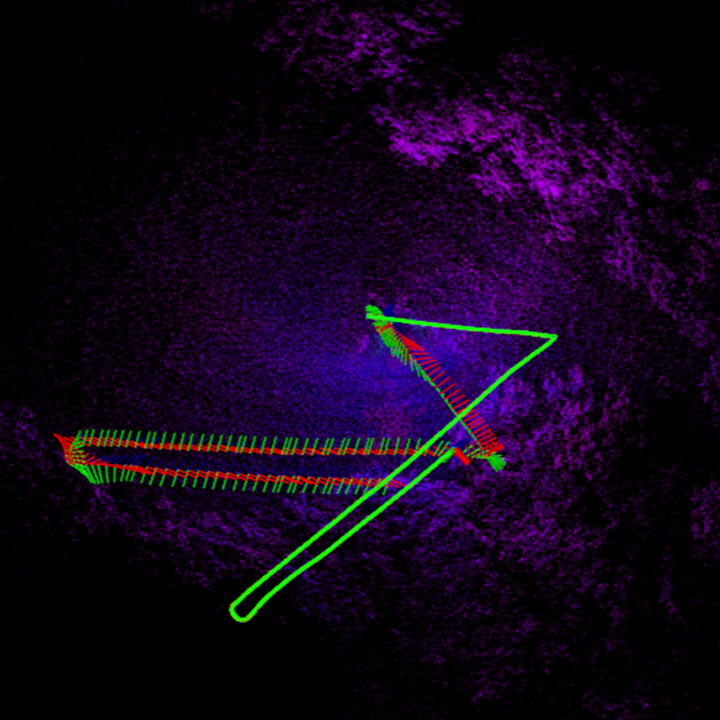
\includegraphics[width=\textwidth]{Included_Images/align_is1.png}
        \caption{Data 1}
    \end{subfigure}
    \hfill
    \begin{subfigure}{0.49\textwidth}
        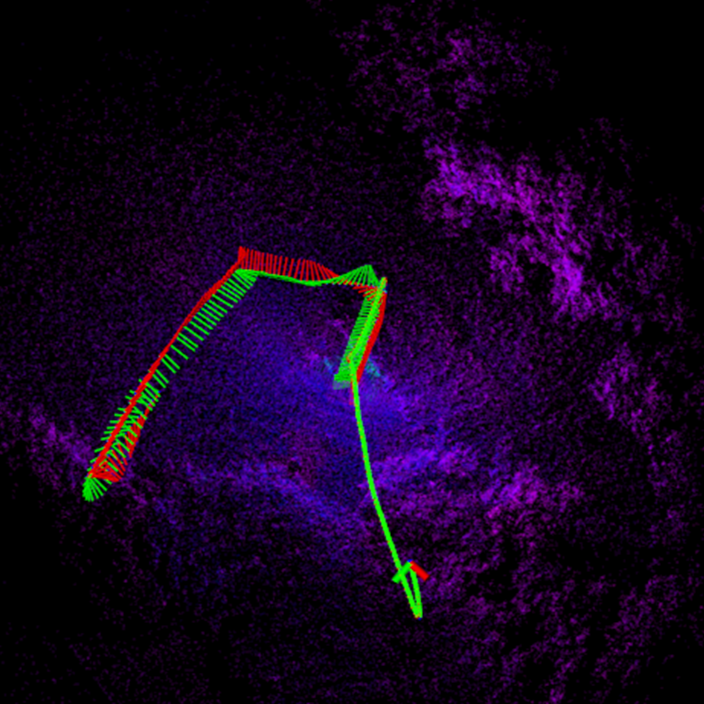
\includegraphics[width=\textwidth]{Included_Images/align_is2.png}
        \caption{Data 2}
    \end{subfigure}
    \caption{Inconsistencies when using fixed calibration information for frame transformation. Green trajectory indicates LiDAR trajectory while the 3-axis trajectory indicated the GPS trajectory.}
\end{figure}


\subsubsection{GNSS-R}
The most common difficulty faced during the project was the inability of
selected GNSS measurement parameters to yield conclusive results. Sometimes this
is caused by the fact that the selected parameters are not sensitive enough to
the ground features, while other times it is caused by noise present in the
dataset. For example, as demonstrated in Figure \ref{GNSS-R Confusing Result},
the plot of $C/N_0$ ratios over FFZs failed to show clear boundaries between
water surfaces, bare soil, and vegetation canopy. This inconsistency with the
clear correlations demonstrated previously in Results and Discussion is caused
by the inclusion of many non-reflected signals received by the bottom antenna.
Particularly, the data included for analysis was contaminated with GNSS signals
received during takeoff and landing, where the proximity between the ground and
the nadir antenna renders it almost impossible for the signals received to be
ground-reflected. 

\begin{figure}[H]
    \centering
    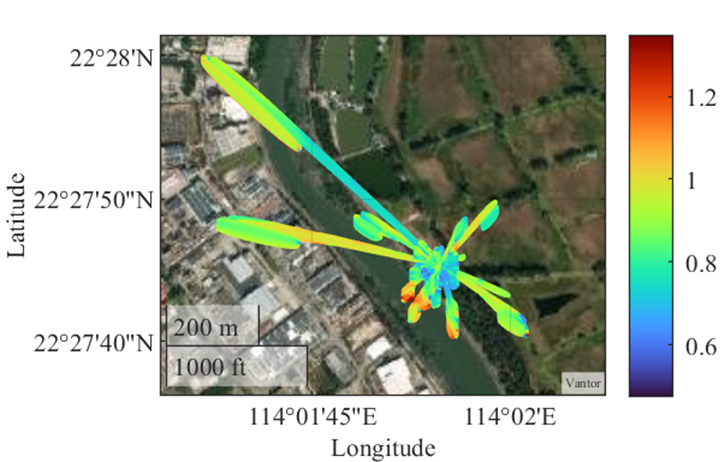
\includegraphics[width=0.75\textwidth]{Included_Images/KeyExperiment_GNSSR.png}
    \caption{Example of unclear correlations observed.}
    \label{GNSS-R Confusing Result}
\end{figure}

After realizing this issue, the data collected during takeoff and landing were
excluded from the GNSS-R processing framework, which ultimately resulted in the
clear correlations demonstrated previously in Results and Discussion. 

Beside the difficulties in obtaining conclusive results, this project was a
continuous trial-and-error process in problem-solving, ranging from debugging
data-processing codes to designing suitable GNSS measurement parameters.
Although time and energy-consuming, this iterative process allowed the extensive
practice of creative and critical thinking, which lies in the heart of the art
of research and makes the entire journey as engaging as possible.

\subsubsection{Machine Learning}
One of the key challenges in developing the Machine Learning based signal classification model was not being able to provide true
ground truth data for training the model. Since any signal level verification was not possible in field conditions the labels were assigned based 
on the experimental scenarios. For example, signals collected in an open sky environment by facing the antenna upwards was labeled as direct signals to the antenna.
However, this method has its own limitations. It introduces a inherent source of noise in the labeling because in practice, the nadir antenna may ocassionally receive direct signals
even when the UAV is hovering at low altitude over bare ground or trees. Same might happen for the upward facing or the zenith antenna. Occassional signals reflected from the ground or trees
can make the dataset noisy for this antenna. This mislabelling is a likely contributor to classification error observed in the confusion matrix. The problem persists particularly
for the boundary cases which share similar characteristics between the classes. 

Furthermore, the class imbalance was another present in the dataset. The data collection scenarios for the tree cases were not equal. The distribution of the satellite geometry also
skewed the dataset for each class. A strategy to balance class weight was applied through the pre processing of the data. Althoug it mitigates teh imbalance to some extent, it does not
remove the skewness or the underlying distribution issue fully. This could made the model overly sensitive to the minority class samples. In future, in order to mitigate the labelling issue
fully, more rigorous data collection can be conducted. One method can be to operate the UAV for longer for data collection with same epoch size for each of the cases. Another strategy could
to stabilise the UAV fully in hovering mode before begining the data collection. 


% --- Appendix ---
\newpage
\addcontentsline{toc}{section}{Appendix}
\section*{Appendix}

\subsubsection*{LiDAR SLAM Pseudocode}
This project builds upon an open-source implementation
that integrates Fast-LIO with PGO for GPS-aided SLAM:
\url{https://github.com/yxw027/FAST_LIO_GPS}. The pseudocode of the front-end and back-end of the modular SLAM can be shown below:
{
    \singlespacing
    \begin{algorithm}[H]
    \caption{Front-End: FAST-LIO with MAVLink TimeSync}
    \begin{algorithmic}[1]
    \State \textbf{Initialize:} IEKF state $\mathbf{x}$ and covariance $\mathbf{P}$
    \State \textbf{Initialize:} ikd-Tree for incremental mapping
    \While{ROS is active}
        \State Sync LiDAR and IMU buffers based on GPS-aligned timestamps
        \If{IMU not initialized}
            \State Perform \textit{IMU\_init} (Gravity/Bias estimation)
            \State \textbf{continue}
        \EndIf
        \State \textbf{State Prediction:} $\hat{\mathbf{x}} \leftarrow$ IMU forward propagation
        \State \textbf{Undistortion:} Compensate point motion using $\hat{\mathbf{x}}$
        \For{$iter = 1$ \textbf{to} $NUM\_MAX\_ITERATIONS$}
            \State Find point-to-plane correspondences in ikd-Tree
            \State Compute measurement residual $\mathbf{z}$ and Jacobian $\mathbf{H}$
            \State \textbf{Update:} Correct state $\mathbf{x}$ using IEKF update rule
            \If{converged} \State \textbf{break} \EndIf
        \EndFor
        \State \textbf{ikd-Tree Update:} Add new features to the spatial map
        \State Publish Odometry to Back-End
    \EndWhile
    \end{algorithmic}
    \end{algorithm}
}
{
    \singlespacing
    \begin{algorithm}[H]
    \caption{Back-End Pose Graph Optimization (PGO)}
    \begin{algorithmic}[1]
    \State \textbf{Initialize:} GTSAM Factor Graph and ISAM2 optimizer
    \State \textbf{Initialize:} Noise models (Odometry, robust GPS, robust Loop)
    \State \textbf{Initialize:} $\text{initial\_z\_yaw}$ as undefined
    \While{ROS is active}
        \State \textbf{Thread 1: Graph Construction (process\_pg)}
        \If{New synchronized Odometry, Point Cloud, and IMU received}
            \State Calculate $\Delta$ movement ($\Delta T, \Delta R$) since last Keyframe
            \If{$\Delta T > \text{KeyframeMeterGap}$ \textbf{or} $\Delta R > \text{KeyframeRadGap}$}
                \State Create new Node $n_k$ in Pose Graph
                \State Generate and save Scan Context for $n_k$
                \State \textbf{Odometry Factor:} Add \textit{BetweenFactor}($n_{k-1}, n_k, \Delta\text{Odom}$)
                
                \If{GPS matched for $n_k$}
                    \State Convert GPS Lat/Lon/Alt to local Cartesian $UTM_{xyz}$
                    \If{$\text{initial\_z\_yaw}$ is undefined}
                        \State Compute and store absolute initial heading from IMU
                    \EndIf
                    \State Apply $Z$-yaw and $X$-tilt offset matrices to $UTM_{xyz}$
                    \If{GPS $X,Y$ covariance $\leq 0.5$}
                        \State \textbf{GPS Factor:} Add 3D \textit{GPSFactor}($n_k, UTM_{x,y,z}$)
                    \Else
                        \State \textbf{GPS Factor:} Add 1D \textit{GPSFactor}($n_k, UTM_z$) \Comment{Trust $Z$-axis only}
                    \EndIf
                \EndIf
            \EndIf
        \EndIf

        \State \textbf{Thread 2: Loop Closure \& ICP (process\_lcd \& process\_icp)}
        \State Search for historical matches using Scan Context
        \If{Loop candidate detected with historical node $n_{\text{old}}$}
            \State Compute relative transform via ICP
            \If{ICP fitness score $<$ Threshold}
                \State \textbf{Loop Factor:} Add \textit{BetweenFactor}($n_{\text{old}}, n_k, T_{\text{ICP}}$)
            \EndIf
        \EndIf
        \State \textbf{Thread 3: Optimization (process\_isam)}
        \State Perform ISAM2 global optimization (\textit{update()} graph \& estimates)
        \State Update global trajectory with optimized poses
    \EndWhile
    \end{algorithmic}
    \end{algorithm}
}

\subsubsection*{Path Planning}

\paragraph{Geometric Shape Factors ($k$)} ~\\
Depending on the boundary shape selected by the algorithm, the corresponding
geometric shape factor is applied to determine the sweeping width:

\begin{table}[H]
    \centering
    \caption{Geometric shape factors used for sweeping distance calculation}
    \label{tab:shape_factors}
    \begin{tabular}{|c|c|}
        \hline
        \textbf{Boundary Shape} & \textbf{Geometric Shape Factor ($k$)} \\
        \hline
        Square   & 1.00 \\
        \hline
        Circle   & 0.89 \\
        \hline
        Triangle & 0.65 \\
        \hline
    \end{tabular}
\end{table}

% --- References ---
\newpage
\addcontentsline{toc}{section}{References}
\bibliographystyle{IEEEtran}
\bibliography{References.bib} 


\end{document}
